\documentclass[a4paper]{scrartcl}
% \documentclass{article}

\usepackage[
fancytheorems, 
fancyproofs, 
noindent, 
%  spacingfix,  
]{adam}

\usepackage{tikz}
\usepackage{bbm}
\usepackage{mathtools}

\title{Graph Theory}
\author{Adam Kelly (\texttt{ak2316@cam.ac.uk})}
\date{\today}


\allowdisplaybreaks

\begin{document}

\maketitle

Graph theory is an area of combinatorics which has lots of fun problems and plenty of interesting theorems.


This article constitutes my notes for the `Graph Theory' course, held in Lent 2021 at Cambridge. These notes are \emph{not a transcription of the lectures}, and differ significantly in quite a few areas. Still, all lectured material should be covered.


\tableofcontents

% \clearpage




\section{Introduction}

For many people, `Graph Theory' is a first course in combinatorics. It's an area with a big focus on problem solving, and it can give a perspective on many other areas of mathematics.  

\subsection{Definitions}

We will begin our course in graph theory naturally by defining what a graph is.

\begin{definition}[Graph]
	A \vocab{graph} is an ordered pair $G = (V, E)$ where $V$ is the set of \vocab{vertices}, and $E \subseteq \{ \{x,y\} \mid x, y \in V, x \neq y \}$ is a set of unordered pairs of vertices called \vocab{edges}.
\end{definition}

We have a natural way of drawing a graph. For each vertex we have a point in the plane, and for each edge we draw a line between the corresponding pair of vertices.

\begin{example}[Example of a Graph]
	The ordered pair $(V, E)$ where $V = \{1, 2, \dots, 6\}$ and $E = \{ \{1, 2\}, \{2, 3\}, \dots, \{5, 6\}\}$ is a graph.
\begin{center}
		

			\tikzset{every picture/.style={line width=0.75pt}} %set default line width to 0.75pt        

			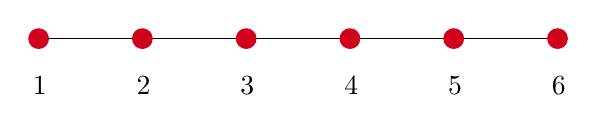
\begin{tikzpicture}[x=0.75pt,y=0.75pt,yscale=-1,xscale=1]
			%uncomment if require: \path (0,300); %set diagram left start at 0, and has height of 300

			%Straight Lines [id:da46250274214576614] 
			\draw    (175,115) -- (425,115) ;
			%Shape: Circle [id:dp08916666481415725] 
			\draw  [draw opacity=0][fill={rgb, 255:red, 208; green, 2; blue, 27 }  ,fill opacity=1 ] (220,115) .. controls (220,112.24) and (222.24,110) .. (225,110) .. controls (227.76,110) and (230,112.24) .. (230,115) .. controls (230,117.76) and (227.76,120) .. (225,120) .. controls (222.24,120) and (220,117.76) .. (220,115) -- cycle ;
			%Shape: Circle [id:dp7997596700799949] 
			\draw  [draw opacity=0][fill={rgb, 255:red, 208; green, 2; blue, 27 }  ,fill opacity=1 ] (270,115) .. controls (270,112.24) and (272.24,110) .. (275,110) .. controls (277.76,110) and (280,112.24) .. (280,115) .. controls (280,117.76) and (277.76,120) .. (275,120) .. controls (272.24,120) and (270,117.76) .. (270,115) -- cycle ;
			%Shape: Circle [id:dp04807433570988917] 
			\draw  [draw opacity=0][fill={rgb, 255:red, 208; green, 2; blue, 27 }  ,fill opacity=1 ] (320,115) .. controls (320,112.24) and (322.24,110) .. (325,110) .. controls (327.76,110) and (330,112.24) .. (330,115) .. controls (330,117.76) and (327.76,120) .. (325,120) .. controls (322.24,120) and (320,117.76) .. (320,115) -- cycle ;
			%Shape: Circle [id:dp6964194673091352] 
			\draw  [draw opacity=0][fill={rgb, 255:red, 208; green, 2; blue, 27 }  ,fill opacity=1 ] (370,115) .. controls (370,112.24) and (372.24,110) .. (375,110) .. controls (377.76,110) and (380,112.24) .. (380,115) .. controls (380,117.76) and (377.76,120) .. (375,120) .. controls (372.24,120) and (370,117.76) .. (370,115) -- cycle ;
			%Shape: Circle [id:dp5929377887646771] 
			\draw  [draw opacity=0][fill={rgb, 255:red, 208; green, 2; blue, 27 }  ,fill opacity=1 ] (420,115) .. controls (420,112.24) and (422.24,110) .. (425,110) .. controls (427.76,110) and (430,112.24) .. (430,115) .. controls (430,117.76) and (427.76,120) .. (425,120) .. controls (422.24,120) and (420,117.76) .. (420,115) -- cycle ;
			%Shape: Circle [id:dp5663003446831361] 
			\draw  [draw opacity=0][fill={rgb, 255:red, 208; green, 2; blue, 27 }  ,fill opacity=1 ] (170,115) .. controls (170,112.24) and (172.24,110) .. (175,110) .. controls (177.76,110) and (180,112.24) .. (180,115) .. controls (180,117.76) and (177.76,120) .. (175,120) .. controls (172.24,120) and (170,117.76) .. (170,115) -- cycle ;

			% Text Node
			\draw (171,132) node [anchor=north west][inner sep=0.75pt]    {$1$};
			% Text Node
			\draw (221,132) node [anchor=north west][inner sep=0.75pt]    {$2$};
			% Text Node
			\draw (271,132) node [anchor=north west][inner sep=0.75pt]    {$3$};
			% Text Node
			\draw (321,132) node [anchor=north west][inner sep=0.75pt]    {$4$};
			% Text Node
			\draw (371,132) node [anchor=north west][inner sep=0.75pt]    {$5$};
			% Text Node
			\draw (421,132) node [anchor=north west][inner sep=0.75pt]    {$6$};


			\end{tikzpicture}

	\end{center}
	This graph is known as $P_6$, a path on 6 vertices.
\end{example}

\subsubsection{Common Graphs}

There are some graphs that will appear repeatedly throughout the course, and we will define them now.

\begin{definition}[Path]
	We define $P_n$ to be the graph 
	$V = \{1, \dots, n\}$, $E = \{\{1, 2\}, \{2, 3\}, \dots, \{n - 1, n\}\}$ as shown.
	\begin{center}
		

			\tikzset{every picture/.style={line width=0.75pt}} %set default line width to 0.75pt        

			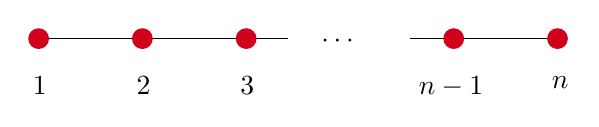
\begin{tikzpicture}[x=0.75pt,y=0.75pt,yscale=-1,xscale=1]
			%uncomment if require: \path (0,93); %set diagram left start at 0, and has height of 93

			%Straight Lines [id:da2966566565444405] 
			\draw    (354,35) -- (425,35) ;
			%Straight Lines [id:da13691249913110026] 
			\draw    (175,35) -- (295,35) ;
			%Shape: Circle [id:dp4038670448284668] 
			\draw  [draw opacity=0][fill={rgb, 255:red, 208; green, 2; blue, 27 }  ,fill opacity=1 ] (220,35) .. controls (220,32.24) and (222.24,30) .. (225,30) .. controls (227.76,30) and (230,32.24) .. (230,35) .. controls (230,37.76) and (227.76,40) .. (225,40) .. controls (222.24,40) and (220,37.76) .. (220,35) -- cycle ;
			%Shape: Circle [id:dp49083678213609794] 
			\draw  [draw opacity=0][fill={rgb, 255:red, 208; green, 2; blue, 27 }  ,fill opacity=1 ] (270,35) .. controls (270,32.24) and (272.24,30) .. (275,30) .. controls (277.76,30) and (280,32.24) .. (280,35) .. controls (280,37.76) and (277.76,40) .. (275,40) .. controls (272.24,40) and (270,37.76) .. (270,35) -- cycle ;
			%Shape: Circle [id:dp06755844317130888] 
			\draw  [draw opacity=0][fill={rgb, 255:red, 208; green, 2; blue, 27 }  ,fill opacity=1 ] (370,35) .. controls (370,32.24) and (372.24,30) .. (375,30) .. controls (377.76,30) and (380,32.24) .. (380,35) .. controls (380,37.76) and (377.76,40) .. (375,40) .. controls (372.24,40) and (370,37.76) .. (370,35) -- cycle ;
			%Shape: Circle [id:dp31955744853716384] 
			\draw  [draw opacity=0][fill={rgb, 255:red, 208; green, 2; blue, 27 }  ,fill opacity=1 ] (420,35) .. controls (420,32.24) and (422.24,30) .. (425,30) .. controls (427.76,30) and (430,32.24) .. (430,35) .. controls (430,37.76) and (427.76,40) .. (425,40) .. controls (422.24,40) and (420,37.76) .. (420,35) -- cycle ;
			%Shape: Circle [id:dp922206172324968] 
			\draw  [draw opacity=0][fill={rgb, 255:red, 208; green, 2; blue, 27 }  ,fill opacity=1 ] (170,35) .. controls (170,32.24) and (172.24,30) .. (175,30) .. controls (177.76,30) and (180,32.24) .. (180,35) .. controls (180,37.76) and (177.76,40) .. (175,40) .. controls (172.24,40) and (170,37.76) .. (170,35) -- cycle ;

			% Text Node
			\draw (171,52) node [anchor=north west][inner sep=0.75pt]    {$1$};
			% Text Node
			\draw (221,52) node [anchor=north west][inner sep=0.75pt]    {$2$};
			% Text Node
			\draw (271,52) node [anchor=north west][inner sep=0.75pt]    {$3$};
			% Text Node
			\draw (357,52) node [anchor=north west][inner sep=0.75pt]    {$n-1$};
			% Text Node
			\draw (421,52) node [anchor=north west][inner sep=0.75pt]    {$n$};
			% Text Node
			\draw (310,32) node [anchor=north west][inner sep=0.75pt]    {$\cdots $};


			\end{tikzpicture}


	\end{center}
	We call this a \vocab{path} on $n$ vertices, and say it has \vocab{length} $n - 1$.
\end{definition}

\begin{definition}[Cycle]
	We define $C_n$ (for $n \geq 3$) to be the graph  $V = \{1, \dots, n\}$, $E = \{ \{1, 2\}, \dots, \{n - 1, n\}, \{n, 1\}\}$ as shown.
	\begin{center}
		
		

\tikzset{every picture/.style={line width=0.75pt}} %set default line width to 0.75pt        

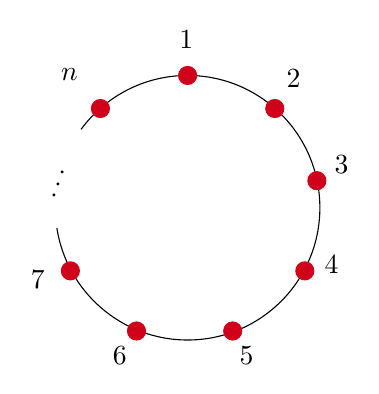
\begin{tikzpicture}[x=0.75pt,y=0.75pt,yscale=-1,xscale=1]
%uncomment if require: \path (0,461); %set diagram left start at 0, and has height of 461

%Shape: Arc [id:dp2939097210495426] 
\draw  [draw opacity=0] (217.92,102.71) .. controls (229.52,86.97) and (248.19,76.75) .. (269.25,76.75) .. controls (304.45,76.75) and (332.98,105.28) .. (332.98,140.48) .. controls (332.98,175.68) and (304.45,204.21) .. (269.25,204.21) .. controls (237.36,204.21) and (210.94,180.77) .. (206.26,150.19) -- (269.25,140.48) -- cycle ; \draw   (217.92,102.71) .. controls (229.52,86.97) and (248.19,76.75) .. (269.25,76.75) .. controls (304.45,76.75) and (332.98,105.28) .. (332.98,140.48) .. controls (332.98,175.68) and (304.45,204.21) .. (269.25,204.21) .. controls (237.36,204.21) and (210.94,180.77) .. (206.26,150.19) ;
%Shape: Ellipse [id:dp08907675877477217] 
\draw  [color={rgb, 255:red, 208; green, 2; blue, 27 }  ,draw opacity=1 ][fill={rgb, 255:red, 208; green, 2; blue, 27 }  ,fill opacity=1 ] (264.91,76.75) .. controls (264.91,74.35) and (266.85,72.41) .. (269.25,72.41) .. controls (271.65,72.41) and (273.6,74.35) .. (273.6,76.75) .. controls (273.6,79.15) and (271.65,81.1) .. (269.25,81.1) .. controls (266.85,81.1) and (264.91,79.15) .. (264.91,76.75) -- cycle ;
%Shape: Ellipse [id:dp6861243810102808] 
\draw  [color={rgb, 255:red, 208; green, 2; blue, 27 }  ,draw opacity=1 ][fill={rgb, 255:red, 208; green, 2; blue, 27 }  ,fill opacity=1 ] (306.91,92.68) .. controls (306.91,90.28) and (308.86,88.34) .. (311.26,88.34) .. controls (313.66,88.34) and (315.6,90.28) .. (315.6,92.68) .. controls (315.6,95.08) and (313.66,97.03) .. (311.26,97.03) .. controls (308.86,97.03) and (306.91,95.08) .. (306.91,92.68) -- cycle ;
%Shape: Circle [id:dp5864785120484053] 
\draw  [color={rgb, 255:red, 208; green, 2; blue, 27 }  ,draw opacity=1 ][fill={rgb, 255:red, 208; green, 2; blue, 27 }  ,fill opacity=1 ] (327.19,127.44) .. controls (327.19,125.04) and (329.13,123.1) .. (331.53,123.1) .. controls (333.93,123.1) and (335.88,125.04) .. (335.88,127.44) .. controls (335.88,129.84) and (333.93,131.79) .. (331.53,131.79) .. controls (329.13,131.79) and (327.19,129.84) .. (327.19,127.44) -- cycle ;
%Shape: Ellipse [id:dp10740847995317393] 
\draw  [color={rgb, 255:red, 208; green, 2; blue, 27 }  ,draw opacity=1 ][fill={rgb, 255:red, 208; green, 2; blue, 27 }  ,fill opacity=1 ] (321.39,170.89) .. controls (321.39,168.5) and (323.34,166.55) .. (325.74,166.55) .. controls (328.14,166.55) and (330.08,168.5) .. (330.08,170.89) .. controls (330.08,173.29) and (328.14,175.24) .. (325.74,175.24) .. controls (323.34,175.24) and (321.39,173.29) .. (321.39,170.89) -- cycle ;
%Shape: Circle [id:dp8188776283145544] 
\draw  [color={rgb, 255:red, 208; green, 2; blue, 27 }  ,draw opacity=1 ][fill={rgb, 255:red, 208; green, 2; blue, 27 }  ,fill opacity=1 ] (286.63,199.86) .. controls (286.63,197.46) and (288.58,195.52) .. (290.98,195.52) .. controls (293.38,195.52) and (295.32,197.46) .. (295.32,199.86) .. controls (295.32,202.26) and (293.38,204.21) .. (290.98,204.21) .. controls (288.58,204.21) and (286.63,202.26) .. (286.63,199.86) -- cycle ;
%Shape: Circle [id:dp20623562846877086] 
\draw  [color={rgb, 255:red, 208; green, 2; blue, 27 }  ,draw opacity=1 ][fill={rgb, 255:red, 208; green, 2; blue, 27 }  ,fill opacity=1 ] (240.29,199.86) .. controls (240.29,197.46) and (242.23,195.52) .. (244.63,195.52) .. controls (247.03,195.52) and (248.98,197.46) .. (248.98,199.86) .. controls (248.98,202.26) and (247.03,204.21) .. (244.63,204.21) .. controls (242.23,204.21) and (240.29,202.26) .. (240.29,199.86) -- cycle ;
%Shape: Ellipse [id:dp8399657424171154] 
\draw  [color={rgb, 255:red, 208; green, 2; blue, 27 }  ,draw opacity=1 ][fill={rgb, 255:red, 208; green, 2; blue, 27 }  ,fill opacity=1 ] (208.42,170.89) .. controls (208.42,168.5) and (210.37,166.55) .. (212.77,166.55) .. controls (215.17,166.55) and (217.11,168.5) .. (217.11,170.89) .. controls (217.11,173.29) and (215.17,175.24) .. (212.77,175.24) .. controls (210.37,175.24) and (208.42,173.29) .. (208.42,170.89) -- cycle ;
%Shape: Rectangle [id:dp758981869824869] 
\draw  [draw opacity=0][fill={rgb, 255:red, 255; green, 255; blue, 255 }  ,fill opacity=0 ] (193.94,99.93) -- (234.49,99.93) -- (234.49,146.27) -- (193.94,146.27) -- cycle ;
%Shape: Ellipse [id:dp07046602779365152] 
\draw  [color={rgb, 255:red, 208; green, 2; blue, 27 }  ,draw opacity=1 ][fill={rgb, 255:red, 208; green, 2; blue, 27 }  ,fill opacity=1 ] (222.91,92.68) .. controls (222.91,90.28) and (224.85,88.34) .. (227.25,88.34) .. controls (229.65,88.34) and (231.6,90.28) .. (231.6,92.68) .. controls (231.6,95.08) and (229.65,97.03) .. (227.25,97.03) .. controls (224.85,97.03) and (222.91,95.08) .. (222.91,92.68) -- cycle ;

% Text Node
\draw (201.99,137.02) node [anchor=north west][inner sep=0.75pt]  [rotate=-289.59]  {$\dotsc $};
% Text Node
\draw (264,54) node [anchor=north west][inner sep=0.75pt]    {$1$};
% Text Node
\draw (315.66,72.55) node [anchor=north west][inner sep=0.75pt]    {$2$};
% Text Node
\draw (338.83,114.1) node [anchor=north west][inner sep=0.75pt]    {$3$};
% Text Node
\draw (334.04,162.45) node [anchor=north west][inner sep=0.75pt]    {$4$};
% Text Node
\draw (293,206) node [anchor=north west][inner sep=0.75pt]    {$5$};
% Text Node
\draw (232.03,206) node [anchor=north west][inner sep=0.75pt]    {$6$};
% Text Node
\draw (192.47,169.45) node [anchor=north west][inner sep=0.75pt]    {$7$};
% Text Node
\draw (207,72) node [anchor=north west][inner sep=0.75pt]    {$n$};


\end{tikzpicture}


	\end{center}
	We call this the \vocab{cycle} on $n$ vertices.
\end{definition}

\begin{definition}[Complete Graph]
	The \vocab{complete graph} on $n$ vertices $K_n$ is the graph $\{1, \dots, n\}$ and $E = \{ \{ i, j \} \mid i \neq j \in V\}$.
	\begin{center}
		

\tikzset{every picture/.style={line width=0.75pt}} %set default line width to 0.75pt        

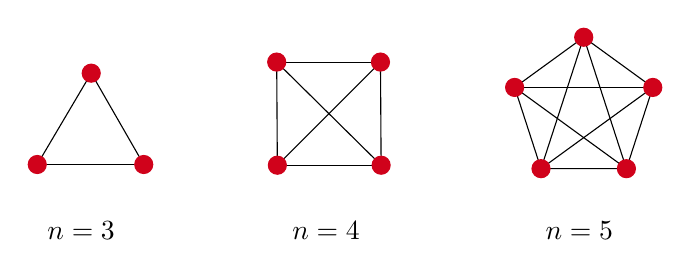
\begin{tikzpicture}[x=0.75pt,y=0.75pt,yscale=-1,xscale=1]
%uncomment if require: \path (0,244); %set diagram left start at 0, and has height of 244

%Straight Lines [id:da9981694225390096] 
\draw    (259.71,56.31) -- (210.02,106) ;
%Straight Lines [id:da26707606947695417] 
\draw    (209.71,56.31) -- (260.02,106) ;
%Straight Lines [id:da6585835091291369] 
\draw    (209.71,56.31) -- (210.02,106) ;
%Straight Lines [id:da7219351678460844] 
\draw    (259.71,56.31) -- (260.02,106) ;
%Straight Lines [id:da0019303873533728089] 
\draw    (209.71,56.31) -- (259.71,56.31) ;
%Straight Lines [id:da7049983363855998] 
\draw    (210.02,106) -- (260.02,106) ;
%Straight Lines [id:da35560926010509697] 
\draw    (120.35,61.65) -- (94.35,105.65) ;
%Straight Lines [id:da7897834071428548] 
\draw    (120.35,61.65) -- (145.65,105.65) ;
%Straight Lines [id:da9938696204324634] 
\draw    (94.35,105.65) -- (145.65,105.65) ;
%Shape: Ellipse [id:dp4113314666492133] 
\draw  [color={rgb, 255:red, 208; green, 2; blue, 27 }  ,draw opacity=1 ][fill={rgb, 255:red, 208; green, 2; blue, 27 }  ,fill opacity=1 ] (90,105.65) .. controls (90,103.26) and (91.95,101.31) .. (94.35,101.31) .. controls (96.74,101.31) and (98.69,103.26) .. (98.69,105.65) .. controls (98.69,108.05) and (96.74,110) .. (94.35,110) .. controls (91.95,110) and (90,108.05) .. (90,105.65) -- cycle ;
%Shape: Ellipse [id:dp834167188739953] 
\draw  [color={rgb, 255:red, 208; green, 2; blue, 27 }  ,draw opacity=1 ][fill={rgb, 255:red, 208; green, 2; blue, 27 }  ,fill opacity=1 ] (141.31,105.65) .. controls (141.31,103.26) and (143.26,101.31) .. (145.65,101.31) .. controls (148.05,101.31) and (150,103.26) .. (150,105.65) .. controls (150,108.05) and (148.05,110) .. (145.65,110) .. controls (143.26,110) and (141.31,108.05) .. (141.31,105.65) -- cycle ;
%Shape: Ellipse [id:dp8095001658436142] 
\draw  [color={rgb, 255:red, 208; green, 2; blue, 27 }  ,draw opacity=1 ][fill={rgb, 255:red, 208; green, 2; blue, 27 }  ,fill opacity=1 ] (116,61.65) .. controls (116,59.26) and (117.95,57.31) .. (120.35,57.31) .. controls (122.74,57.31) and (124.69,59.26) .. (124.69,61.65) .. controls (124.69,64.05) and (122.74,66) .. (120.35,66) .. controls (117.95,66) and (116,64.05) .. (116,61.65) -- cycle ;
%Shape: Ellipse [id:dp10911439146709467] 
\draw  [color={rgb, 255:red, 208; green, 2; blue, 27 }  ,draw opacity=1 ][fill={rgb, 255:red, 208; green, 2; blue, 27 }  ,fill opacity=1 ] (205.37,56.31) .. controls (205.37,53.91) and (207.31,51.96) .. (209.71,51.96) .. controls (212.11,51.96) and (214.06,53.91) .. (214.06,56.31) .. controls (214.06,58.71) and (212.11,60.65) .. (209.71,60.65) .. controls (207.31,60.65) and (205.37,58.71) .. (205.37,56.31) -- cycle ;
%Shape: Ellipse [id:dp8819360357436353] 
\draw  [color={rgb, 255:red, 208; green, 2; blue, 27 }  ,draw opacity=1 ][fill={rgb, 255:red, 208; green, 2; blue, 27 }  ,fill opacity=1 ] (255.37,56.31) .. controls (255.37,53.91) and (257.31,51.96) .. (259.71,51.96) .. controls (262.11,51.96) and (264.06,53.91) .. (264.06,56.31) .. controls (264.06,58.71) and (262.11,60.65) .. (259.71,60.65) .. controls (257.31,60.65) and (255.37,58.71) .. (255.37,56.31) -- cycle ;
%Shape: Ellipse [id:dp05860712986316774] 
\draw  [color={rgb, 255:red, 208; green, 2; blue, 27 }  ,draw opacity=1 ][fill={rgb, 255:red, 208; green, 2; blue, 27 }  ,fill opacity=1 ] (205.68,106) .. controls (205.68,103.6) and (207.62,101.65) .. (210.02,101.65) .. controls (212.42,101.65) and (214.37,103.6) .. (214.37,106) .. controls (214.37,108.4) and (212.42,110.35) .. (210.02,110.35) .. controls (207.62,110.35) and (205.68,108.4) .. (205.68,106) -- cycle ;
%Shape: Ellipse [id:dp5283352169897437] 
\draw  [color={rgb, 255:red, 208; green, 2; blue, 27 }  ,draw opacity=1 ][fill={rgb, 255:red, 208; green, 2; blue, 27 }  ,fill opacity=1 ] (255.68,106) .. controls (255.68,103.6) and (257.62,101.65) .. (260.02,101.65) .. controls (262.42,101.65) and (264.37,103.6) .. (264.37,106) .. controls (264.37,108.4) and (262.42,110.35) .. (260.02,110.35) .. controls (257.62,110.35) and (255.68,108.4) .. (255.68,106) -- cycle ;
%Shape: Regular Polygon [id:dp10308828814670479] 
\draw   (357.63,44.35) -- (390.92,68.53) -- (378.2,107.66) -- (337.06,107.66) -- (324.35,68.53) -- cycle ;
%Straight Lines [id:da43627704398128486] 
\draw    (324.35,68.53) -- (378.2,107.66) ;
%Straight Lines [id:da0011702067257907123] 
\draw    (337.06,107.66) -- (390.92,68.53) ;
%Straight Lines [id:da9427395129530866] 
\draw    (337.06,107.66) -- (357.63,44.35) ;
%Straight Lines [id:da7244564555034867] 
\draw    (324.35,68.53) -- (390.92,68.53) ;
%Straight Lines [id:da6627152022664105] 
\draw    (357.63,44.35) -- (378.2,107.66) ;
%Shape: Ellipse [id:dp7300400411305249] 
\draw  [color={rgb, 255:red, 208; green, 2; blue, 27 }  ,draw opacity=1 ][fill={rgb, 255:red, 208; green, 2; blue, 27 }  ,fill opacity=1 ] (353.29,44.35) .. controls (353.29,41.95) and (355.23,40) .. (357.63,40) .. controls (360.03,40) and (361.98,41.95) .. (361.98,44.35) .. controls (361.98,46.74) and (360.03,48.69) .. (357.63,48.69) .. controls (355.23,48.69) and (353.29,46.74) .. (353.29,44.35) -- cycle ;
%Shape: Ellipse [id:dp8020435268234443] 
\draw  [color={rgb, 255:red, 208; green, 2; blue, 27 }  ,draw opacity=1 ][fill={rgb, 255:red, 208; green, 2; blue, 27 }  ,fill opacity=1 ] (320,68.53) .. controls (320,66.13) and (321.95,64.18) .. (324.35,64.18) .. controls (326.74,64.18) and (328.69,66.13) .. (328.69,68.53) .. controls (328.69,70.93) and (326.74,72.87) .. (324.35,72.87) .. controls (321.95,72.87) and (320,70.93) .. (320,68.53) -- cycle ;
%Shape: Ellipse [id:dp5063058740897554] 
\draw  [color={rgb, 255:red, 208; green, 2; blue, 27 }  ,draw opacity=1 ][fill={rgb, 255:red, 208; green, 2; blue, 27 }  ,fill opacity=1 ] (332.71,107.66) .. controls (332.71,105.26) and (334.66,103.32) .. (337.06,103.32) .. controls (339.46,103.32) and (341.4,105.26) .. (341.4,107.66) .. controls (341.4,110.06) and (339.46,112.01) .. (337.06,112.01) .. controls (334.66,112.01) and (332.71,110.06) .. (332.71,107.66) -- cycle ;
%Shape: Ellipse [id:dp20023345004172588] 
\draw  [color={rgb, 255:red, 208; green, 2; blue, 27 }  ,draw opacity=1 ][fill={rgb, 255:red, 208; green, 2; blue, 27 }  ,fill opacity=1 ] (373.86,107.66) .. controls (373.86,105.26) and (375.8,103.32) .. (378.2,103.32) .. controls (380.6,103.32) and (382.55,105.26) .. (382.55,107.66) .. controls (382.55,110.06) and (380.6,112.01) .. (378.2,112.01) .. controls (375.8,112.01) and (373.86,110.06) .. (373.86,107.66) -- cycle ;
%Shape: Ellipse [id:dp34706748597281534] 
\draw  [color={rgb, 255:red, 208; green, 2; blue, 27 }  ,draw opacity=1 ][fill={rgb, 255:red, 208; green, 2; blue, 27 }  ,fill opacity=1 ] (386.57,68.53) .. controls (386.57,66.13) and (388.52,64.18) .. (390.92,64.18) .. controls (393.32,64.18) and (395.26,66.13) .. (395.26,68.53) .. controls (395.26,70.93) and (393.32,72.87) .. (390.92,72.87) .. controls (388.52,72.87) and (386.57,70.93) .. (386.57,68.53) -- cycle ;

% Text Node
\draw (98,132) node [anchor=north west][inner sep=0.75pt]    {$n=3$};
% Text Node
\draw (216,132) node [anchor=north west][inner sep=0.75pt]    {$n=4$};
% Text Node
\draw (338,132) node [anchor=north west][inner sep=0.75pt]    {$n=5$};


\end{tikzpicture}

	\end{center}
	Note that there is an edge between every pair of vertices.
\end{definition}

\begin{definition}[Empty Graph]
	We define the \vocab{empty graph} on $n$ vertices $\overline{K_n}$ to have $V = \{1, \dots, n\}$ but $E = \emptyset$.
\end{definition}

\begin{remark}
	In our definition of a graph, we {\itshape don't allow} loops, and there {\itshape cannot} be multiple edges between the same set of vertices.
	\begin{center}
		

\tikzset{every picture/.style={line width=0.75pt}} %set default line width to 0.75pt        

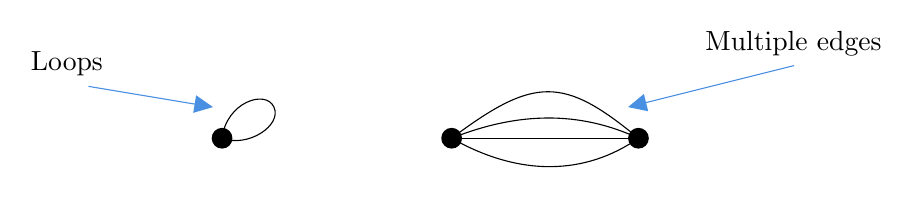
\begin{tikzpicture}[x=0.75pt,y=0.75pt,yscale=-1,xscale=1]
%uncomment if require: \path (0,93); %set diagram left start at 0, and has height of 93

%Curve Lines [id:da2865357772607766] 
\draw    (194.39,55) .. controls (196.39,37.75) and (215.39,31.25) .. (219.39,40) .. controls (223.39,48.75) and (206.89,59.75) .. (194.39,55) -- cycle ;
%Shape: Circle [id:dp0229132580239656] 
\draw  [draw opacity=0][fill={rgb, 255:red, 0; green, 0; blue, 0 }  ,fill opacity=1 ] (189.39,55) .. controls (189.39,52.24) and (191.63,50) .. (194.39,50) .. controls (197.15,50) and (199.39,52.24) .. (199.39,55) .. controls (199.39,57.76) and (197.15,60) .. (194.39,60) .. controls (191.63,60) and (189.39,57.76) .. (189.39,55) -- cycle ;
%Shape: Circle [id:dp1638222573350646] 
\draw  [draw opacity=0][fill={rgb, 255:red, 0; green, 0; blue, 0 }  ,fill opacity=1 ] (300,55) .. controls (300,52.24) and (302.24,50) .. (305,50) .. controls (307.76,50) and (310,52.24) .. (310,55) .. controls (310,57.76) and (307.76,60) .. (305,60) .. controls (302.24,60) and (300,57.76) .. (300,55) -- cycle ;
%Shape: Circle [id:dp537703730076633] 
\draw  [draw opacity=0][fill={rgb, 255:red, 0; green, 0; blue, 0 }  ,fill opacity=1 ] (390,55) .. controls (390,52.24) and (392.24,50) .. (395,50) .. controls (397.76,50) and (400,52.24) .. (400,55) .. controls (400,57.76) and (397.76,60) .. (395,60) .. controls (392.24,60) and (390,57.76) .. (390,55) -- cycle ;
%Straight Lines [id:da6617588206410779] 
\draw    (305,55) -- (395,55) ;
%Curve Lines [id:da23655718519286506] 
\draw    (305,55) .. controls (345,25) and (359,25.25) .. (395,55) ;
%Curve Lines [id:da6706610581979621] 
\draw    (305,55) .. controls (337,42.25) and (366.5,41.75) .. (395,55) ;
%Curve Lines [id:da14619136331292015] 
\draw    (305,55) .. controls (338,73.75) and (369.5,72.75) .. (395,55) ;
%Straight Lines [id:da03138886450780565] 
\draw [color={rgb, 255:red, 74; green, 144; blue, 226 }  ,draw opacity=1 ]   (130,30) -- (187.04,39.51) ;
\draw [shift={(190,40)}, rotate = 189.46] [fill={rgb, 255:red, 74; green, 144; blue, 226 }  ,fill opacity=1 ][line width=0.08]  [draw opacity=0] (8.93,-4.29) -- (0,0) -- (8.93,4.29) -- cycle    ;
%Straight Lines [id:da17643117622964488] 
\draw [color={rgb, 255:red, 74; green, 144; blue, 226 }  ,draw opacity=1 ]   (470,20) -- (392.91,39.27) ;
\draw [shift={(390,40)}, rotate = 345.96000000000004] [fill={rgb, 255:red, 74; green, 144; blue, 226 }  ,fill opacity=1 ][line width=0.08]  [draw opacity=0] (8.93,-4.29) -- (0,0) -- (8.93,4.29) -- cycle    ;

% Text Node
\draw (101,12) node [anchor=north west][inner sep=0.75pt]   [align=left] {Loops};
% Text Node
\draw (426,2) node [anchor=north west][inner sep=0.75pt]   [align=left] {Multiple edges};


\end{tikzpicture}

	\end{center}
	These limitations are inherent in our definition, where we use sets rather than multisets. You can define graphs where such things are allowed, but for now we will outlaw them. We also note that edges are \emph{unordered pairs}, so for now edges have no direction.
\end{remark}

To be slightly more succinct, we will use some shorthand notation. 

\begin{notation}
If $G = (V, E)$ is a graph, and we have some edge $\{x, y\} \in E$, we will denote it by $xy$. We will also define $|G| = |V|$, and $e(G) = |E|$.
\end{notation}
 
\begin{example}[Vertices and Edges of $K_n$]
	Consider the graph $K_n$. We have $|K_n| = n$, and $e(K_n) = \binom{k}{2}$, as there is an edge between any pair of vertices.
\end{example}

\subsubsection{Subgraphs}

Now we will define the notion of a \emph{subgraph}, in the natural way.

\begin{definition}[Subgraph]
	We say that $H= (V', E')$ is a \vocab{subgraph} of $G = (V, E)$ if $V' \subseteq V$ and $E' \subseteq E$.
\end{definition}

Informally, $H$ is a subgraph of $G$ if we can remove vertices and edges from $G$ to get $H$. Let's look at some examples.

\begin{example}[Example of a Subgraph]
	The graph on the right is a subgraph of the graph on the left.
\begin{center}
	

\tikzset{every picture/.style={line width=0.75pt}} %set default line width to 0.75pt        

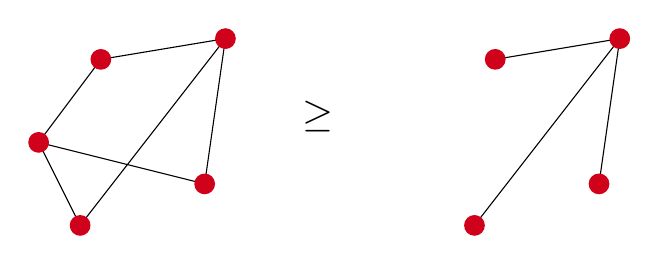
\begin{tikzpicture}[x=0.75pt,y=0.75pt,yscale=-1,xscale=1]
%uncomment if require: \path (0,193); %set diagram left start at 0, and has height of 193

%Straight Lines [id:da5102818539821388] 
\draw    (145,75) -- (175,35) ;
%Straight Lines [id:da11653049971761209] 
\draw    (235,25) -- (175,35) ;
%Straight Lines [id:da5706156443747223] 
\draw    (235,25) -- (225,95) ;
%Straight Lines [id:da9053001100461334] 
\draw    (145,75) -- (165,115) ;
%Straight Lines [id:da5994949539529218] 
\draw    (235,25) -- (165,115) ;
%Straight Lines [id:da2071898142257198] 
\draw    (225,95) -- (145,75) ;
%Shape: Circle [id:dp7335328414030793] 
\draw  [draw opacity=0][fill={rgb, 255:red, 208; green, 2; blue, 27 }  ,fill opacity=1 ] (170,35) .. controls (170,32.24) and (172.24,30) .. (175,30) .. controls (177.76,30) and (180,32.24) .. (180,35) .. controls (180,37.76) and (177.76,40) .. (175,40) .. controls (172.24,40) and (170,37.76) .. (170,35) -- cycle ;
%Shape: Circle [id:dp25158480193801747] 
\draw  [draw opacity=0][fill={rgb, 255:red, 208; green, 2; blue, 27 }  ,fill opacity=1 ] (140,75) .. controls (140,72.24) and (142.24,70) .. (145,70) .. controls (147.76,70) and (150,72.24) .. (150,75) .. controls (150,77.76) and (147.76,80) .. (145,80) .. controls (142.24,80) and (140,77.76) .. (140,75) -- cycle ;
%Shape: Circle [id:dp7366774963822135] 
\draw  [draw opacity=0][fill={rgb, 255:red, 208; green, 2; blue, 27 }  ,fill opacity=1 ] (160,115) .. controls (160,112.24) and (162.24,110) .. (165,110) .. controls (167.76,110) and (170,112.24) .. (170,115) .. controls (170,117.76) and (167.76,120) .. (165,120) .. controls (162.24,120) and (160,117.76) .. (160,115) -- cycle ;
%Shape: Circle [id:dp986170211009179] 
\draw  [draw opacity=0][fill={rgb, 255:red, 208; green, 2; blue, 27 }  ,fill opacity=1 ] (220,95) .. controls (220,92.24) and (222.24,90) .. (225,90) .. controls (227.76,90) and (230,92.24) .. (230,95) .. controls (230,97.76) and (227.76,100) .. (225,100) .. controls (222.24,100) and (220,97.76) .. (220,95) -- cycle ;
%Shape: Circle [id:dp08748002464606974] 
\draw  [draw opacity=0][fill={rgb, 255:red, 208; green, 2; blue, 27 }  ,fill opacity=1 ] (230,25) .. controls (230,22.24) and (232.24,20) .. (235,20) .. controls (237.76,20) and (240,22.24) .. (240,25) .. controls (240,27.76) and (237.76,30) .. (235,30) .. controls (232.24,30) and (230,27.76) .. (230,25) -- cycle ;
%Straight Lines [id:da6558038306138124] 
\draw    (425,25) -- (365,35) ;
%Straight Lines [id:da22960999678468086] 
\draw    (425,25) -- (415,95) ;
%Straight Lines [id:da3699284235556677] 
\draw    (425,25) -- (355,115) ;
%Shape: Circle [id:dp31621516337124767] 
\draw  [draw opacity=0][fill={rgb, 255:red, 208; green, 2; blue, 27 }  ,fill opacity=1 ] (360,35) .. controls (360,32.24) and (362.24,30) .. (365,30) .. controls (367.76,30) and (370,32.24) .. (370,35) .. controls (370,37.76) and (367.76,40) .. (365,40) .. controls (362.24,40) and (360,37.76) .. (360,35) -- cycle ;
%Shape: Circle [id:dp3827184917507753] 
\draw  [draw opacity=0][fill={rgb, 255:red, 208; green, 2; blue, 27 }  ,fill opacity=1 ] (350,115) .. controls (350,112.24) and (352.24,110) .. (355,110) .. controls (357.76,110) and (360,112.24) .. (360,115) .. controls (360,117.76) and (357.76,120) .. (355,120) .. controls (352.24,120) and (350,117.76) .. (350,115) -- cycle ;
%Shape: Circle [id:dp10694204690570841] 
\draw  [draw opacity=0][fill={rgb, 255:red, 208; green, 2; blue, 27 }  ,fill opacity=1 ] (410,95) .. controls (410,92.24) and (412.24,90) .. (415,90) .. controls (417.76,90) and (420,92.24) .. (420,95) .. controls (420,97.76) and (417.76,100) .. (415,100) .. controls (412.24,100) and (410,97.76) .. (410,95) -- cycle ;
%Shape: Circle [id:dp9708117128742255] 
\draw  [draw opacity=0][fill={rgb, 255:red, 208; green, 2; blue, 27 }  ,fill opacity=1 ] (420,25) .. controls (420,22.24) and (422.24,20) .. (425,20) .. controls (427.76,20) and (430,22.24) .. (430,25) .. controls (430,27.76) and (427.76,30) .. (425,30) .. controls (422.24,30) and (420,27.76) .. (420,25) -- cycle ;

% Text Node
\draw (271,54) node [anchor=north west][inner sep=0.75pt]  [font=\Large]  {$\geq $};


\end{tikzpicture}

\end{center}

\end{example}

We are also going to use some notation for removing an edge or a vertex from a graph. Of course, when removing a vertex you also have to remove the edges connecting to it.


\begin{notation}[Adding/Removing Vertices \& Edges]
	For an edge $xy$ or a vertex $x$, we define $G - xy$ to be the graph $G$ with the edge $xy$ removed, and $G - x$ to be $G$ with vertex $x$ removed, along with all edges incident to $x$. We will also define $G + xy$ to be $G$ with the edge $xy$, and $G + x$ to be $G$ with the vertex $x$. 
\end{notation}

An easy way to get a subgraph is by taking a subset of the vertices and seeing what edges you get from the original graph.

\begin{definition}[Inducted Subgraph]
	If $G = (V, E)$ is a graph and $X \subseteq V$, the \vocab{subgraph inducted by $X$} is defined to be $G[X] = (X, \{xy \in E \mid x, y \in X\})$.
\end{definition}

\subsubsection{Graph Isomorphism}

Now that we have defined graphs, it's natural to define some notion of isomorphism.

\begin{definition}[Graph Isomorphism]
	Let $G = (V, E)$ and $H = (V', E')$ be graphs. We say that $f : V \rightarrow V'$ is a \vocab{graph isomorphism} if $f(u)f(v) \in E' \iff uv \in E$. 

	If there is a graph isomorphism between $G$ and $H$ then we say they are \vocab{isomorphic}.
\end{definition}

Now for the following discussion, fix some graph $G = (V, E)$, and let $x \in V$. 

\begin{definition}[Neighbourhood]
	If $xy \in E$, then we say that $x$ and $y$ are \vocab{adjacent}.
	We define the \vocab{neighborhood} of $x$ to be the set $N(x) = \{ y \in V \mid xy \in E\}$ of all vertices adjacent to $x$.
\end{definition}

Note that as in the diagram below, $x$ is not in its own neighborhood.
\begin{center}
	

\tikzset{every picture/.style={line width=0.75pt}} %set default line width to 0.75pt        

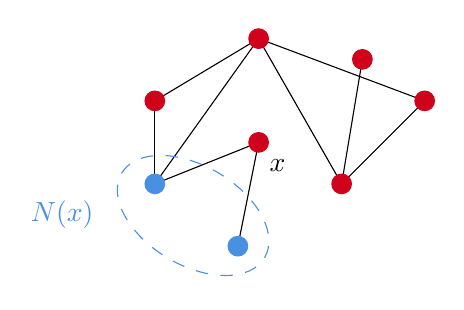
\begin{tikzpicture}[x=0.75pt,y=0.75pt,yscale=-1,xscale=1]
%uncomment if require: \path (0,193); %set diagram left start at 0, and has height of 193

%Straight Lines [id:da9588865668616432] 
\draw    (275,35) -- (225,65) ;
%Straight Lines [id:da6040267926385874] 
\draw    (325,45) -- (315,105) ;
%Straight Lines [id:da2949070003151344] 
\draw    (275,85) -- (265,135) ;
%Straight Lines [id:da20743790772148674] 
\draw    (225,105) -- (275,85) ;
%Straight Lines [id:da4910146433079081] 
\draw    (225,105) -- (225,65) ;
%Straight Lines [id:da5820247237359314] 
\draw    (225,105) -- (275,35) ;
%Straight Lines [id:da5614914262150004] 
\draw    (275,35) -- (315,105) ;
%Straight Lines [id:da23660182919629502] 
\draw    (355,65) -- (275,35) ;
%Straight Lines [id:da18662720934380073] 
\draw    (355,65) -- (315,105) ;
%Shape: Circle [id:dp7796053805504014] 
\draw  [draw opacity=0][fill={rgb, 255:red, 208; green, 2; blue, 27 }  ,fill opacity=1 ] (220,65) .. controls (220,62.24) and (222.24,60) .. (225,60) .. controls (227.76,60) and (230,62.24) .. (230,65) .. controls (230,67.76) and (227.76,70) .. (225,70) .. controls (222.24,70) and (220,67.76) .. (220,65) -- cycle ;
%Shape: Circle [id:dp5410193836574619] 
\draw  [draw opacity=0][fill={rgb, 255:red, 208; green, 2; blue, 27 }  ,fill opacity=1 ] (270,35) .. controls (270,32.24) and (272.24,30) .. (275,30) .. controls (277.76,30) and (280,32.24) .. (280,35) .. controls (280,37.76) and (277.76,40) .. (275,40) .. controls (272.24,40) and (270,37.76) .. (270,35) -- cycle ;
%Shape: Circle [id:dp7645390851559083] 
\draw  [draw opacity=0][fill={rgb, 255:red, 208; green, 2; blue, 27 }  ,fill opacity=1 ] (320,45) .. controls (320,42.24) and (322.24,40) .. (325,40) .. controls (327.76,40) and (330,42.24) .. (330,45) .. controls (330,47.76) and (327.76,50) .. (325,50) .. controls (322.24,50) and (320,47.76) .. (320,45) -- cycle ;
%Shape: Circle [id:dp2737498580146679] 
\draw  [draw opacity=0][fill={rgb, 255:red, 74; green, 144; blue, 226 }  ,fill opacity=1 ] (220,105) .. controls (220,102.24) and (222.24,100) .. (225,100) .. controls (227.76,100) and (230,102.24) .. (230,105) .. controls (230,107.76) and (227.76,110) .. (225,110) .. controls (222.24,110) and (220,107.76) .. (220,105) -- cycle ;
%Shape: Circle [id:dp8649705530172823] 
\draw  [draw opacity=0][fill={rgb, 255:red, 208; green, 2; blue, 27 }  ,fill opacity=1 ] (270,85) .. controls (270,82.24) and (272.24,80) .. (275,80) .. controls (277.76,80) and (280,82.24) .. (280,85) .. controls (280,87.76) and (277.76,90) .. (275,90) .. controls (272.24,90) and (270,87.76) .. (270,85) -- cycle ;
%Shape: Circle [id:dp37860744340197594] 
\draw  [draw opacity=0][fill={rgb, 255:red, 208; green, 2; blue, 27 }  ,fill opacity=1 ] (310,105) .. controls (310,102.24) and (312.24,100) .. (315,100) .. controls (317.76,100) and (320,102.24) .. (320,105) .. controls (320,107.76) and (317.76,110) .. (315,110) .. controls (312.24,110) and (310,107.76) .. (310,105) -- cycle ;
%Shape: Circle [id:dp16994333406917272] 
\draw  [draw opacity=0][fill={rgb, 255:red, 74; green, 144; blue, 226 }  ,fill opacity=1 ] (260,135) .. controls (260,132.24) and (262.24,130) .. (265,130) .. controls (267.76,130) and (270,132.24) .. (270,135) .. controls (270,137.76) and (267.76,140) .. (265,140) .. controls (262.24,140) and (260,137.76) .. (260,135) -- cycle ;
%Shape: Circle [id:dp7574466548746062] 
\draw  [draw opacity=0][fill={rgb, 255:red, 208; green, 2; blue, 27 }  ,fill opacity=1 ] (350,65) .. controls (350,62.24) and (352.24,60) .. (355,60) .. controls (357.76,60) and (360,62.24) .. (360,65) .. controls (360,67.76) and (357.76,70) .. (355,70) .. controls (352.24,70) and (350,67.76) .. (350,65) -- cycle ;
%Shape: Ellipse [id:dp42082831262373377] 
\draw  [color={rgb, 255:red, 74; green, 144; blue, 226 }  ,draw opacity=1 ][dash pattern={on 4.5pt off 4.5pt}] (208.98,99.87) .. controls (215.68,88.53) and (236.53,88.43) .. (255.56,99.66) .. controls (274.58,110.89) and (284.57,129.2) .. (277.87,140.55) .. controls (271.17,151.9) and (250.31,151.99) .. (231.29,140.76) .. controls (212.27,129.53) and (202.28,111.22) .. (208.98,99.87) -- cycle ;

% Text Node
\draw (279,92) node [anchor=north west][inner sep=0.75pt]    {$x$};
% Text Node
\draw (164,112) node [anchor=north west][inner sep=0.75pt]  [color={rgb, 255:red, 74; green, 144; blue, 226 }  ,opacity=1 ]  {$N( x)$};


\end{tikzpicture}

\end{center}

\begin{definition}[Degree]
	We define the \vocab{degree} of a vertex $x$ to be $d(x) = |N(x)|$. This is equal to the number of edges that are incident to $x$.
\end{definition}

% Now for some graph $G$ with vertices $V = \{x_1, \dots, x_n\}$, we say the \vocab{degree sequence} of $G$ is $d(x_1), d(x_2), \dots, d(x_n)$.

\begin{definition}[Regularity]
	A graph $G$ is said to be \vocab{regular} if all of the degrees are the same. We say $G$ is $k$-regular if $d(x) = k$ for all $x \in V$.
\end{definition}

\begin{example}[Regular and Non-Regular Graphs]
	The graphs $K_n$ is $n - 1$ regular, and $C_n$ is $2$-regular.
	The graph $P_n$ is not regular.
\end{example}

\subsubsection{Connectivity}

We now want to define some notion of \emph{connectivity}, where a vertex $u$ is connected to vertex $v$ if you can follow some path in the graph to get from $u$ to $v$.

\begin{center}

	

\tikzset{every picture/.style={line width=0.75pt}} %set default line width to 0.75pt        

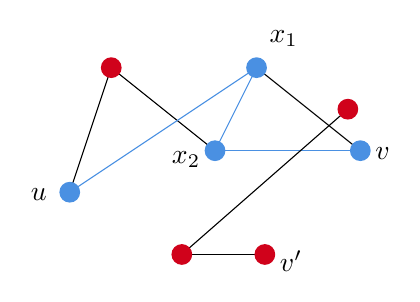
\begin{tikzpicture}[x=0.75pt,y=0.75pt,yscale=-1,xscale=1]
%uncomment if require: \path (0,193); %set diagram left start at 0, and has height of 193

%Straight Lines [id:da622057432821673] 
\draw    (211,75) -- (231,15) ;
%Straight Lines [id:da45132208780914207] 
\draw    (231,15) -- (281,55) ;
%Straight Lines [id:da30820364060918315] 
\draw [color={rgb, 255:red, 74; green, 144; blue, 226 }  ,draw opacity=1 ]   (301,15) -- (281,55) ;
%Straight Lines [id:da8027434077669512] 
\draw [color={rgb, 255:red, 74; green, 144; blue, 226 }  ,draw opacity=1 ]   (351,55) -- (281,55) ;
%Straight Lines [id:da16630547460303047] 
\draw [color={rgb, 255:red, 74; green, 144; blue, 226 }  ,draw opacity=1 ]   (301,15) -- (211,75) ;
%Straight Lines [id:da9414715970752923] 
\draw    (351,55) -- (301,15) ;
%Straight Lines [id:da009376398482458415] 
\draw    (345,35) -- (265,105) ;
%Straight Lines [id:da8452379949704987] 
\draw    (305,105) -- (265,105) ;
%Shape: Circle [id:dp8926415649677933] 
\draw  [draw opacity=0][fill={rgb, 255:red, 208; green, 2; blue, 27 }  ,fill opacity=1 ] (226,15) .. controls (226,12.24) and (228.24,10) .. (231,10) .. controls (233.76,10) and (236,12.24) .. (236,15) .. controls (236,17.76) and (233.76,20) .. (231,20) .. controls (228.24,20) and (226,17.76) .. (226,15) -- cycle ;
%Shape: Circle [id:dp06866505571224346] 
\draw  [draw opacity=0][fill={rgb, 255:red, 74; green, 144; blue, 226 }  ,fill opacity=1 ] (296,15) .. controls (296,12.24) and (298.24,10) .. (301,10) .. controls (303.76,10) and (306,12.24) .. (306,15) .. controls (306,17.76) and (303.76,20) .. (301,20) .. controls (298.24,20) and (296,17.76) .. (296,15) -- cycle ;
%Shape: Circle [id:dp3115374601380443] 
\draw  [draw opacity=0][fill={rgb, 255:red, 74; green, 144; blue, 226 }  ,fill opacity=1 ] (206,75) .. controls (206,72.24) and (208.24,70) .. (211,70) .. controls (213.76,70) and (216,72.24) .. (216,75) .. controls (216,77.76) and (213.76,80) .. (211,80) .. controls (208.24,80) and (206,77.76) .. (206,75) -- cycle ;
%Shape: Circle [id:dp14211747814115727] 
\draw  [draw opacity=0][fill={rgb, 255:red, 74; green, 144; blue, 226 }  ,fill opacity=1 ] (346,55) .. controls (346,52.24) and (348.24,50) .. (351,50) .. controls (353.76,50) and (356,52.24) .. (356,55) .. controls (356,57.76) and (353.76,60) .. (351,60) .. controls (348.24,60) and (346,57.76) .. (346,55) -- cycle ;
%Shape: Circle [id:dp9991626952144155] 
\draw  [draw opacity=0][fill={rgb, 255:red, 74; green, 144; blue, 226 }  ,fill opacity=1 ] (276,55) .. controls (276,52.24) and (278.24,50) .. (281,50) .. controls (283.76,50) and (286,52.24) .. (286,55) .. controls (286,57.76) and (283.76,60) .. (281,60) .. controls (278.24,60) and (276,57.76) .. (276,55) -- cycle ;
%Shape: Circle [id:dp5747900065455143] 
\draw  [draw opacity=0][fill={rgb, 255:red, 208; green, 2; blue, 27 }  ,fill opacity=1 ] (300,105) .. controls (300,102.24) and (302.24,100) .. (305,100) .. controls (307.76,100) and (310,102.24) .. (310,105) .. controls (310,107.76) and (307.76,110) .. (305,110) .. controls (302.24,110) and (300,107.76) .. (300,105) -- cycle ;
%Shape: Circle [id:dp13737323142390678] 
\draw  [draw opacity=0][fill={rgb, 255:red, 208; green, 2; blue, 27 }  ,fill opacity=1 ] (260,105) .. controls (260,102.24) and (262.24,100) .. (265,100) .. controls (267.76,100) and (270,102.24) .. (270,105) .. controls (270,107.76) and (267.76,110) .. (265,110) .. controls (262.24,110) and (260,107.76) .. (260,105) -- cycle ;
%Shape: Circle [id:dp04201057706920763] 
\draw  [draw opacity=0][fill={rgb, 255:red, 208; green, 2; blue, 27 }  ,fill opacity=1 ] (340,35) .. controls (340,32.24) and (342.24,30) .. (345,30) .. controls (347.76,30) and (350,32.24) .. (350,35) .. controls (350,37.76) and (347.76,40) .. (345,40) .. controls (342.24,40) and (340,37.76) .. (340,35) -- cycle ;

% Text Node
\draw (191,72) node [anchor=north west][inner sep=0.75pt]    {$u$};
% Text Node
\draw (357,52) node [anchor=north west][inner sep=0.75pt]    {$v$};
% Text Node
\draw (311,102) node [anchor=north west][inner sep=0.75pt]    {$v'$};
% Text Node
\draw (259,54) node [anchor=north west][inner sep=0.75pt]    {$x_{2}$};
% Text Node
\draw (306,-4) node [anchor=north west][inner sep=0.75pt]    {$x_{1}$};


\end{tikzpicture}


\end{center}

For example, in the graph above we want to say somehow that $u$ and $v$ are connected, but $u$ and $v'$ are not. To do this, we will introduce some more definitions.

\begin{definition}[$uv$ Path]
	A \vocab{$uv$ path} is a sequence $x_1, x_2, \dots, x_l$ where $x_1, \dots, x_l$ are distinct, $x_1 = u$, $x_l = v$ and $x_i x_{i + 1} \in E$.
\end{definition}

In the example above, $u x_1 x_2 v$ is a $uv$ path. 

The slight subtlety in this condition is the \emph{distinctness} condition. For example, if $x_1 \dots x_l$ is a $uv$ path and $y_1 \dots y_{l'}$ is a $vw$ path, then $x_1 \dots x_l y_1 \dots y_{l'}$ may \emph{not} be a $uw$ path since we may have reused an edge. Of course, we can just not reuse edges by avoiding cycles.

\begin{proposition}[Joining Paths]
	If $x_1 \dots x_l$ is a $uv$ path and $y_1 \dots y_{l'}$ is a $vw$ path, then $x_1 \dots x_l y_1 \dots y_{l'}$ contains a $uw$ path.
\end{proposition}
\begin{proof}
	Choose a minimal subsequence $w_1 \dots w_r$ of $x_1 \dots x_l y_1 \dots y_{l'}$ such that
	\begin{enumerate}
		\item $w_i w_{i + 1} \in E$.
		\item $w_1 = u$, $w_r = w$.
	\end{enumerate}
	We now claim that $w_1 \dots w_r$ is a $uw$ path. If this was not the case, then it must fail on distinctness, so there would exist some $z$ such that the sequence is
	$$
	w_1 \dots w_{a} z w_{a + 2} \dots w_b z w_{b + 2} w_r,
	$$
	but now note that
	$$
	w_1 \dots w_{a}zw_{b+2} \dots w_r
	$$
	also satisfies the conditions for the subsequence, but is strictly shorter length. This contradicts the minimality condition.
\end{proof}

Now given $G = (V, E)$, let's define an equivalence relation $\sim$ on $V$, where
$$
x \sim y \iff \text{there exists an $xy$ path in $G$}.
$$

\begin{proposition}
	$\sim$ is an equivalence relation.
\end{proposition}
\begin{proof}
	Note that $\sim$ is reflexive and symmetric, and we get transitivity from our previous proposition.
\end{proof}


\begin{example}
	In the graph below, the vertices that are the same colour are in the same equivalence class under $\sim$.
	\begin{center}
		

\tikzset{every picture/.style={line width=0.75pt}} %set default line width to 0.75pt        

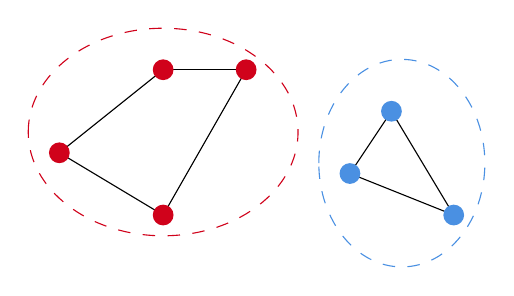
\begin{tikzpicture}[x=0.75pt,y=0.75pt,yscale=-1,xscale=1]
%uncomment if require: \path (0,193); %set diagram left start at 0, and has height of 193

%Straight Lines [id:da026420751885910643] 
\draw    (235,55) -- (185,95) ;
%Straight Lines [id:da9722690765704908] 
\draw    (275,55) -- (235,55) ;
%Straight Lines [id:da06843618607928192] 
\draw    (235,125) -- (275,55) ;
%Straight Lines [id:da5625605688196442] 
\draw    (185,95) -- (235,125) ;
%Straight Lines [id:da988200478921885] 
\draw    (325,105) -- (345,75) ;
%Straight Lines [id:da911347603435119] 
\draw    (375,125) -- (345,75) ;
%Straight Lines [id:da8522085082708648] 
\draw    (375,125) -- (325,105) ;
%Shape: Circle [id:dp6731202040761254] 
\draw  [draw opacity=0][fill={rgb, 255:red, 74; green, 144; blue, 226 }  ,fill opacity=1 ] (320,105) .. controls (320,102.24) and (322.24,100) .. (325,100) .. controls (327.76,100) and (330,102.24) .. (330,105) .. controls (330,107.76) and (327.76,110) .. (325,110) .. controls (322.24,110) and (320,107.76) .. (320,105) -- cycle ;
%Shape: Circle [id:dp6918700817283945] 
\draw  [draw opacity=0][fill={rgb, 255:red, 74; green, 144; blue, 226 }  ,fill opacity=1 ] (340,75) .. controls (340,72.24) and (342.24,70) .. (345,70) .. controls (347.76,70) and (350,72.24) .. (350,75) .. controls (350,77.76) and (347.76,80) .. (345,80) .. controls (342.24,80) and (340,77.76) .. (340,75) -- cycle ;
%Shape: Circle [id:dp8990189535612337] 
\draw  [draw opacity=0][fill={rgb, 255:red, 74; green, 144; blue, 226 }  ,fill opacity=1 ] (370,125) .. controls (370,122.24) and (372.24,120) .. (375,120) .. controls (377.76,120) and (380,122.24) .. (380,125) .. controls (380,127.76) and (377.76,130) .. (375,130) .. controls (372.24,130) and (370,127.76) .. (370,125) -- cycle ;
%Shape: Circle [id:dp5598547497180938] 
\draw  [draw opacity=0][fill={rgb, 255:red, 208; green, 2; blue, 27 }  ,fill opacity=1 ] (230,55) .. controls (230,52.24) and (232.24,50) .. (235,50) .. controls (237.76,50) and (240,52.24) .. (240,55) .. controls (240,57.76) and (237.76,60) .. (235,60) .. controls (232.24,60) and (230,57.76) .. (230,55) -- cycle ;
%Shape: Circle [id:dp38539457383955944] 
\draw  [draw opacity=0][fill={rgb, 255:red, 208; green, 2; blue, 27 }  ,fill opacity=1 ] (180,95) .. controls (180,92.24) and (182.24,90) .. (185,90) .. controls (187.76,90) and (190,92.24) .. (190,95) .. controls (190,97.76) and (187.76,100) .. (185,100) .. controls (182.24,100) and (180,97.76) .. (180,95) -- cycle ;
%Shape: Circle [id:dp7818087689592826] 
\draw  [draw opacity=0][fill={rgb, 255:red, 208; green, 2; blue, 27 }  ,fill opacity=1 ] (230,125) .. controls (230,122.24) and (232.24,120) .. (235,120) .. controls (237.76,120) and (240,122.24) .. (240,125) .. controls (240,127.76) and (237.76,130) .. (235,130) .. controls (232.24,130) and (230,127.76) .. (230,125) -- cycle ;
%Shape: Circle [id:dp7622426997206498] 
\draw  [draw opacity=0][fill={rgb, 255:red, 208; green, 2; blue, 27 }  ,fill opacity=1 ] (270,55) .. controls (270,52.24) and (272.24,50) .. (275,50) .. controls (277.76,50) and (280,52.24) .. (280,55) .. controls (280,57.76) and (277.76,60) .. (275,60) .. controls (272.24,60) and (270,57.76) .. (270,55) -- cycle ;
%Shape: Ellipse [id:dp39967148726972657] 
\draw  [color={rgb, 255:red, 208; green, 2; blue, 27 }  ,draw opacity=1 ][dash pattern={on 4.5pt off 4.5pt}] (170,85) .. controls (170,57.39) and (199.1,35) .. (235,35) .. controls (270.9,35) and (300,57.39) .. (300,85) .. controls (300,112.61) and (270.9,135) .. (235,135) .. controls (199.1,135) and (170,112.61) .. (170,85) -- cycle ;
%Shape: Ellipse [id:dp994417464374959] 
\draw  [color={rgb, 255:red, 74; green, 144; blue, 226 }  ,draw opacity=1 ][dash pattern={on 4.5pt off 4.5pt}] (310,100) .. controls (310,72.39) and (327.91,50) .. (350,50) .. controls (372.09,50) and (390,72.39) .. (390,100) .. controls (390,127.61) and (372.09,150) .. (350,150) .. controls (327.91,150) and (310,127.61) .. (310,100) -- cycle ;




\end{tikzpicture}

	\end{center}
\end{example}

\begin{definition}[Connected Graph]
If there is a path between any two vertices in $G$ then we say that $G$ is \vocab{connected}.	
\end{definition}

\begin{definition}[Connected Components]
We call the equivalence classes of $\sim$ on $G$ the \vocab{components} or \vocab{connected components} of $G$.
\end{definition}

\subsubsection{Edges and Distance}

We can also introduce some useful definitions relating to the edges of a graph.

\begin{definition}[Minimum/Maximum Degree]
	Let $G$ be a graph. The \vocab{maximum degree} of $G$, $\triangle(G)$ is defined to be $\triangle(G) = \max_{x \in V} d(x)$. Similarly, we define the \vocab{minimum degree} of $G$, $\delta(G)$ to be $\delta(G) = \min_{x \in V} d(x)$.
\end{definition}

In a $k$-regular graph as mentioned above, we have $\triangle(G) = \delta(G) = k$.

\begin{definition}[Graph Distance]
Let $G = (V, E)$ be a graph. The associated \vocab{graph distance} $d: V \times V \rightarrow \R^{\geq 0} \cup \{ \infty \}$ is defined so that $d(x, y)$ is the minimum path length from $x$ to $y$ if it exists, and $\infty$ otherwise.
\end{definition}

\begin{proposition}[Graph Distance is a Metric]
	Let $G = (V, E)$ be a connected graph and let $d$ be the associated graph distance. Then $(V, d)$ defines a metric space.
\end{proposition}
\begin{proof}[Proof Sketch]
	We have $d(x, y) = 0$, and $d(x, y) = d(y, x)$ (taking the shortest path in the opposite direction), and $d(x, z) \leq d(x, y) + d(y, z)$ as we can find path from $x$ to $z$ by taking paths from $x$ to $y$ and $y$ to $z$ and adjoining them, and this puts an upper bound on $d(x, z)$.
\end{proof}

\subsection{Trees}

We will now discuss a special class of graph called \emph{trees}.
This class is quite restrictive (yet is quite useful), and they have some nice properties.

To define what a tree is, we first need a notion of when a graph is acyclic.

\begin{definition}[Acyclic]
	A graph $G$ is said to be \vocab{acyclic} if it does not contain any subgraph isomorphic to a cycle, $C_n$.
\end{definition}

\begin{example}[Example of Acyclic/Non-Acyclic Graphs]
	In the example below, the two graphs are both \emph{acyclic}.
	\begin{center}


		\tikzset{every picture/.style={line width=0.75pt}} %set default line width to 0.75pt        

		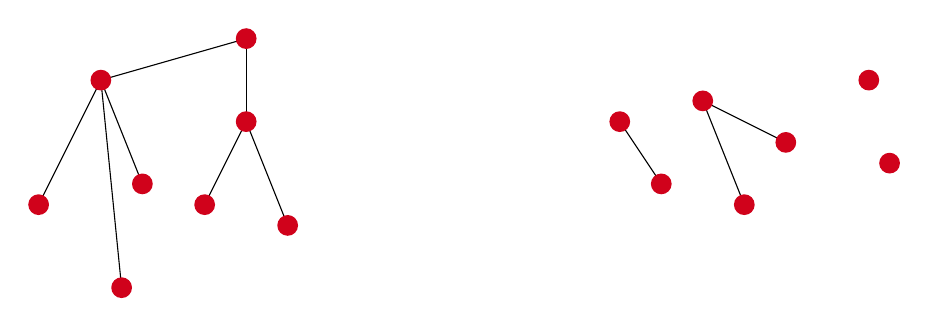
\begin{tikzpicture}[x=0.75pt,y=0.75pt,yscale=-1,xscale=1]
		%uncomment if require: \path (0,193); %set diagram left start at 0, and has height of 193
		
		%Straight Lines [id:da4975879578224476] 
		\draw    (195,25) -- (125,45) ;
		%Straight Lines [id:da9875182002621871] 
		\draw    (195,25) -- (195,65) ;
		%Straight Lines [id:da14692421279536638] 
		\draw    (125,45) -- (145,95) ;
		%Straight Lines [id:da5597906353336949] 
		\draw    (125,45) -- (135,145) ;
		%Straight Lines [id:da827590697469549] 
		\draw    (125,45) -- (95,105) ;
		%Straight Lines [id:da24566898686094285] 
		\draw    (195,65) -- (175,105) ;
		%Straight Lines [id:da013473140578307952] 
		\draw    (195,65) -- (215,115) ;
		%Shape: Circle [id:dp017139343550431563] 
		\draw  [draw opacity=0][fill={rgb, 255:red, 208; green, 2; blue, 27 }  ,fill opacity=1 ] (120,45) .. controls (120,42.24) and (122.24,40) .. (125,40) .. controls (127.76,40) and (130,42.24) .. (130,45) .. controls (130,47.76) and (127.76,50) .. (125,50) .. controls (122.24,50) and (120,47.76) .. (120,45) -- cycle ;
		%Shape: Circle [id:dp9218534791001208] 
		\draw  [draw opacity=0][fill={rgb, 255:red, 208; green, 2; blue, 27 }  ,fill opacity=1 ] (190,25) .. controls (190,22.24) and (192.24,20) .. (195,20) .. controls (197.76,20) and (200,22.24) .. (200,25) .. controls (200,27.76) and (197.76,30) .. (195,30) .. controls (192.24,30) and (190,27.76) .. (190,25) -- cycle ;
		%Shape: Circle [id:dp2781242473026011] 
		\draw  [draw opacity=0][fill={rgb, 255:red, 208; green, 2; blue, 27 }  ,fill opacity=1 ] (190,65) .. controls (190,62.24) and (192.24,60) .. (195,60) .. controls (197.76,60) and (200,62.24) .. (200,65) .. controls (200,67.76) and (197.76,70) .. (195,70) .. controls (192.24,70) and (190,67.76) .. (190,65) -- cycle ;
		%Shape: Circle [id:dp030803892200315652] 
		\draw  [draw opacity=0][fill={rgb, 255:red, 208; green, 2; blue, 27 }  ,fill opacity=1 ] (90,105) .. controls (90,102.24) and (92.24,100) .. (95,100) .. controls (97.76,100) and (100,102.24) .. (100,105) .. controls (100,107.76) and (97.76,110) .. (95,110) .. controls (92.24,110) and (90,107.76) .. (90,105) -- cycle ;
		%Shape: Circle [id:dp05177451328998328] 
		\draw  [draw opacity=0][fill={rgb, 255:red, 208; green, 2; blue, 27 }  ,fill opacity=1 ] (130,145) .. controls (130,142.24) and (132.24,140) .. (135,140) .. controls (137.76,140) and (140,142.24) .. (140,145) .. controls (140,147.76) and (137.76,150) .. (135,150) .. controls (132.24,150) and (130,147.76) .. (130,145) -- cycle ;
		%Shape: Circle [id:dp9829721568494545] 
		\draw  [draw opacity=0][fill={rgb, 255:red, 208; green, 2; blue, 27 }  ,fill opacity=1 ] (140,95) .. controls (140,92.24) and (142.24,90) .. (145,90) .. controls (147.76,90) and (150,92.24) .. (150,95) .. controls (150,97.76) and (147.76,100) .. (145,100) .. controls (142.24,100) and (140,97.76) .. (140,95) -- cycle ;
		%Shape: Circle [id:dp41010913556293216] 
		\draw  [draw opacity=0][fill={rgb, 255:red, 208; green, 2; blue, 27 }  ,fill opacity=1 ] (210,115) .. controls (210,112.24) and (212.24,110) .. (215,110) .. controls (217.76,110) and (220,112.24) .. (220,115) .. controls (220,117.76) and (217.76,120) .. (215,120) .. controls (212.24,120) and (210,117.76) .. (210,115) -- cycle ;
		%Shape: Circle [id:dp2845228574030323] 
		\draw  [draw opacity=0][fill={rgb, 255:red, 208; green, 2; blue, 27 }  ,fill opacity=1 ] (170,105) .. controls (170,102.24) and (172.24,100) .. (175,100) .. controls (177.76,100) and (180,102.24) .. (180,105) .. controls (180,107.76) and (177.76,110) .. (175,110) .. controls (172.24,110) and (170,107.76) .. (170,105) -- cycle ;
		%Straight Lines [id:da3465675313818486] 
		\draw    (415,55) -- (435,105) ;
		%Shape: Circle [id:dp4803286610625792] 
		\draw  [draw opacity=0][fill={rgb, 255:red, 208; green, 2; blue, 27 }  ,fill opacity=1 ] (430,105) .. controls (430,102.24) and (432.24,100) .. (435,100) .. controls (437.76,100) and (440,102.24) .. (440,105) .. controls (440,107.76) and (437.76,110) .. (435,110) .. controls (432.24,110) and (430,107.76) .. (430,105) -- cycle ;
		%Straight Lines [id:da21407762828429155] 
		\draw    (415,55) -- (455,75) ;
		%Shape: Circle [id:dp6332637183866524] 
		\draw  [draw opacity=0][fill={rgb, 255:red, 208; green, 2; blue, 27 }  ,fill opacity=1 ] (450,75) .. controls (450,72.24) and (452.24,70) .. (455,70) .. controls (457.76,70) and (460,72.24) .. (460,75) .. controls (460,77.76) and (457.76,80) .. (455,80) .. controls (452.24,80) and (450,77.76) .. (450,75) -- cycle ;
		%Shape: Circle [id:dp7070779056968607] 
		\draw  [draw opacity=0][fill={rgb, 255:red, 208; green, 2; blue, 27 }  ,fill opacity=1 ] (410,55) .. controls (410,52.24) and (412.24,50) .. (415,50) .. controls (417.76,50) and (420,52.24) .. (420,55) .. controls (420,57.76) and (417.76,60) .. (415,60) .. controls (412.24,60) and (410,57.76) .. (410,55) -- cycle ;
		%Shape: Circle [id:dp5461528770985675] 
		\draw  [draw opacity=0][fill={rgb, 255:red, 208; green, 2; blue, 27 }  ,fill opacity=1 ] (500,85) .. controls (500,82.24) and (502.24,80) .. (505,80) .. controls (507.76,80) and (510,82.24) .. (510,85) .. controls (510,87.76) and (507.76,90) .. (505,90) .. controls (502.24,90) and (500,87.76) .. (500,85) -- cycle ;
		%Shape: Circle [id:dp2134597956334484] 
		\draw  [draw opacity=0][fill={rgb, 255:red, 208; green, 2; blue, 27 }  ,fill opacity=1 ] (490,45) .. controls (490,42.24) and (492.24,40) .. (495,40) .. controls (497.76,40) and (500,42.24) .. (500,45) .. controls (500,47.76) and (497.76,50) .. (495,50) .. controls (492.24,50) and (490,47.76) .. (490,45) -- cycle ;
		%Straight Lines [id:da9266795704990405] 
		\draw    (375,65) -- (395,95) ;
		%Shape: Circle [id:dp5484535938793745] 
		\draw  [draw opacity=0][fill={rgb, 255:red, 208; green, 2; blue, 27 }  ,fill opacity=1 ] (390,95) .. controls (390,92.24) and (392.24,90) .. (395,90) .. controls (397.76,90) and (400,92.24) .. (400,95) .. controls (400,97.76) and (397.76,100) .. (395,100) .. controls (392.24,100) and (390,97.76) .. (390,95) -- cycle ;
		%Shape: Circle [id:dp9664538152744377] 
		\draw  [draw opacity=0][fill={rgb, 255:red, 208; green, 2; blue, 27 }  ,fill opacity=1 ] (370,65) .. controls (370,62.24) and (372.24,60) .. (375,60) .. controls (377.76,60) and (380,62.24) .. (380,65) .. controls (380,67.76) and (377.76,70) .. (375,70) .. controls (372.24,70) and (370,67.76) .. (370,65) -- cycle ;
		
		
		
		
		\end{tikzpicture}
		
	\end{center}
Two \emph{non-acyclic} graphs are shown below. The subgraphs isomorphic to $C_4$ and $C_3$ are highlighted.
\begin{center}
	\tikzset{every picture/.style={line width=0.75pt}} %set default line width to 0.75pt        

	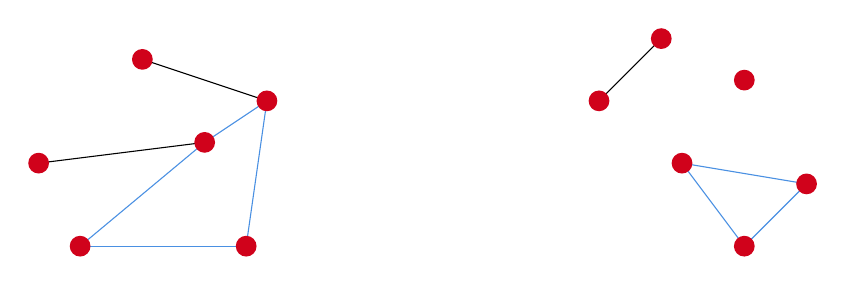
\begin{tikzpicture}[x=0.75pt,y=0.75pt,yscale=-1,xscale=1]
	%uncomment if require: \path (0,193); %set diagram left start at 0, and has height of 193
	
	%Shape: Circle [id:dp866182978887481] 
	\draw  [draw opacity=0][fill={rgb, 255:red, 208; green, 2; blue, 27 }  ,fill opacity=1 ] (490,45) .. controls (490,42.24) and (492.24,40) .. (495,40) .. controls (497.76,40) and (500,42.24) .. (500,45) .. controls (500,47.76) and (497.76,50) .. (495,50) .. controls (492.24,50) and (490,47.76) .. (490,45) -- cycle ;
	%Straight Lines [id:da3990958073757699] 
	\draw    (205,35) -- (265,55) ;
	%Straight Lines [id:da9365392145712541] 
	\draw    (155,85) -- (235,75) ;
	%Straight Lines [id:da5851899106406085] 
	\draw [color={rgb, 255:red, 74; green, 144; blue, 226 }  ,draw opacity=1 ]   (175,125) -- (255,125) ;
	%Straight Lines [id:da6407598405676712] 
	\draw [color={rgb, 255:red, 74; green, 144; blue, 226 }  ,draw opacity=1 ]   (175,125) -- (235,75) ;
	%Straight Lines [id:da8200458164877145] 
	\draw [color={rgb, 255:red, 74; green, 144; blue, 226 }  ,draw opacity=1 ]   (235,75) -- (265,55) ;
	%Straight Lines [id:da340128979084815] 
	\draw [color={rgb, 255:red, 74; green, 144; blue, 226 }  ,draw opacity=1 ]   (255,125) -- (265,55) ;
	%Shape: Circle [id:dp22572431620923994] 
	\draw  [draw opacity=0][fill={rgb, 255:red, 208; green, 2; blue, 27 }  ,fill opacity=1 ] (200,35) .. controls (200,32.24) and (202.24,30) .. (205,30) .. controls (207.76,30) and (210,32.24) .. (210,35) .. controls (210,37.76) and (207.76,40) .. (205,40) .. controls (202.24,40) and (200,37.76) .. (200,35) -- cycle ;
	%Shape: Circle [id:dp1543865759025298] 
	\draw  [draw opacity=0][fill={rgb, 255:red, 208; green, 2; blue, 27 }  ,fill opacity=1 ] (150,85) .. controls (150,82.24) and (152.24,80) .. (155,80) .. controls (157.76,80) and (160,82.24) .. (160,85) .. controls (160,87.76) and (157.76,90) .. (155,90) .. controls (152.24,90) and (150,87.76) .. (150,85) -- cycle ;
	%Shape: Circle [id:dp5753092419464733] 
	\draw  [draw opacity=0][fill={rgb, 255:red, 208; green, 2; blue, 27 }  ,fill opacity=1 ] (230,75) .. controls (230,72.24) and (232.24,70) .. (235,70) .. controls (237.76,70) and (240,72.24) .. (240,75) .. controls (240,77.76) and (237.76,80) .. (235,80) .. controls (232.24,80) and (230,77.76) .. (230,75) -- cycle ;
	%Shape: Circle [id:dp6003377360697513] 
	\draw  [draw opacity=0][fill={rgb, 255:red, 208; green, 2; blue, 27 }  ,fill opacity=1 ] (170,125) .. controls (170,122.24) and (172.24,120) .. (175,120) .. controls (177.76,120) and (180,122.24) .. (180,125) .. controls (180,127.76) and (177.76,130) .. (175,130) .. controls (172.24,130) and (170,127.76) .. (170,125) -- cycle ;
	%Shape: Circle [id:dp06975091279440304] 
	\draw  [draw opacity=0][fill={rgb, 255:red, 208; green, 2; blue, 27 }  ,fill opacity=1 ] (260,55) .. controls (260,52.24) and (262.24,50) .. (265,50) .. controls (267.76,50) and (270,52.24) .. (270,55) .. controls (270,57.76) and (267.76,60) .. (265,60) .. controls (262.24,60) and (260,57.76) .. (260,55) -- cycle ;
	%Shape: Circle [id:dp094055476422784] 
	\draw  [draw opacity=0][fill={rgb, 255:red, 208; green, 2; blue, 27 }  ,fill opacity=1 ] (250,125) .. controls (250,122.24) and (252.24,120) .. (255,120) .. controls (257.76,120) and (260,122.24) .. (260,125) .. controls (260,127.76) and (257.76,130) .. (255,130) .. controls (252.24,130) and (250,127.76) .. (250,125) -- cycle ;
	%Straight Lines [id:da49187362873904295] 
	\draw    (425,55) -- (455,25) ;
	%Straight Lines [id:da6165790041655467] 
	\draw [color={rgb, 255:red, 74; green, 144; blue, 226 }  ,draw opacity=1 ]   (495,125) -- (525,95) ;
	%Straight Lines [id:da25398744826879927] 
	\draw [color={rgb, 255:red, 74; green, 144; blue, 226 }  ,draw opacity=1 ]   (495,125) -- (465,85) ;
	%Straight Lines [id:da6473275212261544] 
	\draw [color={rgb, 255:red, 74; green, 144; blue, 226 }  ,draw opacity=1 ]   (525,95) -- (465,85) ;
	%Shape: Circle [id:dp6644211842344737] 
	\draw  [draw opacity=0][fill={rgb, 255:red, 208; green, 2; blue, 27 }  ,fill opacity=1 ] (450,25) .. controls (450,22.24) and (452.24,20) .. (455,20) .. controls (457.76,20) and (460,22.24) .. (460,25) .. controls (460,27.76) and (457.76,30) .. (455,30) .. controls (452.24,30) and (450,27.76) .. (450,25) -- cycle ;
	%Shape: Circle [id:dp3296386978476522] 
	\draw  [draw opacity=0][fill={rgb, 255:red, 208; green, 2; blue, 27 }  ,fill opacity=1 ] (460,85) .. controls (460,82.24) and (462.24,80) .. (465,80) .. controls (467.76,80) and (470,82.24) .. (470,85) .. controls (470,87.76) and (467.76,90) .. (465,90) .. controls (462.24,90) and (460,87.76) .. (460,85) -- cycle ;
	%Shape: Circle [id:dp9908699544980412] 
	\draw  [draw opacity=0][fill={rgb, 255:red, 208; green, 2; blue, 27 }  ,fill opacity=1 ] (420,55) .. controls (420,52.24) and (422.24,50) .. (425,50) .. controls (427.76,50) and (430,52.24) .. (430,55) .. controls (430,57.76) and (427.76,60) .. (425,60) .. controls (422.24,60) and (420,57.76) .. (420,55) -- cycle ;
	%Shape: Circle [id:dp8971260082042065] 
	\draw  [draw opacity=0][fill={rgb, 255:red, 208; green, 2; blue, 27 }  ,fill opacity=1 ] (520,95) .. controls (520,92.24) and (522.24,90) .. (525,90) .. controls (527.76,90) and (530,92.24) .. (530,95) .. controls (530,97.76) and (527.76,100) .. (525,100) .. controls (522.24,100) and (520,97.76) .. (520,95) -- cycle ;
	%Shape: Circle [id:dp5125506334648022] 
	\draw  [draw opacity=0][fill={rgb, 255:red, 208; green, 2; blue, 27 }  ,fill opacity=1 ] (490,125) .. controls (490,122.24) and (492.24,120) .. (495,120) .. controls (497.76,120) and (500,122.24) .. (500,125) .. controls (500,127.76) and (497.76,130) .. (495,130) .. controls (492.24,130) and (490,127.76) .. (490,125) -- cycle ;
	
	
	
	
	\end{tikzpicture}
	

\end{center}
\end{example}

\begin{definition}[Tree]
	A \vocab{tree} is a connected, acyclic graph.
\end{definition}

\begin{example}[Examples of Trees]
	The following three graphs are trees.
	\begin{center}
		

\tikzset{every picture/.style={line width=0.75pt}} %set default line width to 0.75pt        

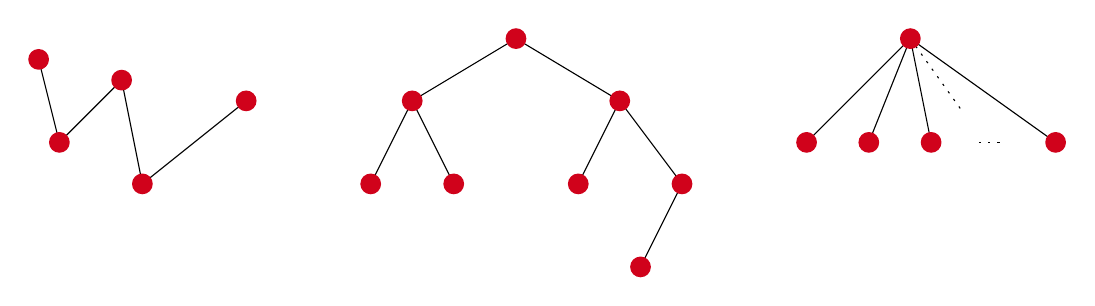
\begin{tikzpicture}[x=0.75pt,y=0.75pt,yscale=-1,xscale=1]
%uncomment if require: \path (0,193); %set diagram left start at 0, and has height of 193

%Straight Lines [id:da49703614339776037] 
\draw  [dash pattern={on 0.84pt off 2.51pt}]  (545,25) -- (570,60) ;
%Straight Lines [id:da8560002704789386] 
\draw    (545,25) -- (495,75) ;
%Straight Lines [id:da8111128726222414] 
\draw    (545,25) -- (525,75) ;
%Straight Lines [id:da706792274923423] 
\draw    (545,25) -- (555,75) ;
%Straight Lines [id:da46674031153499496] 
\draw    (545,25) -- (615,75) ;
%Straight Lines [id:da2902373414033316] 
\draw    (125,35) -- (135,75) ;
%Straight Lines [id:da9385080584462927] 
\draw    (135,75) -- (165,45) ;
%Straight Lines [id:da6001851670749982] 
\draw    (175,95) -- (165,45) ;
%Straight Lines [id:da6179902147981986] 
\draw    (175,95) -- (225,55) ;
%Shape: Circle [id:dp7325026650910265] 
\draw  [draw opacity=0][fill={rgb, 255:red, 208; green, 2; blue, 27 }  ,fill opacity=1 ] (120,35) .. controls (120,32.24) and (122.24,30) .. (125,30) .. controls (127.76,30) and (130,32.24) .. (130,35) .. controls (130,37.76) and (127.76,40) .. (125,40) .. controls (122.24,40) and (120,37.76) .. (120,35) -- cycle ;
%Shape: Circle [id:dp611790102044747] 
\draw  [draw opacity=0][fill={rgb, 255:red, 208; green, 2; blue, 27 }  ,fill opacity=1 ] (130,75) .. controls (130,72.24) and (132.24,70) .. (135,70) .. controls (137.76,70) and (140,72.24) .. (140,75) .. controls (140,77.76) and (137.76,80) .. (135,80) .. controls (132.24,80) and (130,77.76) .. (130,75) -- cycle ;
%Shape: Circle [id:dp3596636072841959] 
\draw  [draw opacity=0][fill={rgb, 255:red, 208; green, 2; blue, 27 }  ,fill opacity=1 ] (160,45) .. controls (160,42.24) and (162.24,40) .. (165,40) .. controls (167.76,40) and (170,42.24) .. (170,45) .. controls (170,47.76) and (167.76,50) .. (165,50) .. controls (162.24,50) and (160,47.76) .. (160,45) -- cycle ;
%Shape: Circle [id:dp7908891047683889] 
\draw  [draw opacity=0][fill={rgb, 255:red, 208; green, 2; blue, 27 }  ,fill opacity=1 ] (170,95) .. controls (170,92.24) and (172.24,90) .. (175,90) .. controls (177.76,90) and (180,92.24) .. (180,95) .. controls (180,97.76) and (177.76,100) .. (175,100) .. controls (172.24,100) and (170,97.76) .. (170,95) -- cycle ;
%Shape: Circle [id:dp5262181762220665] 
\draw  [draw opacity=0][fill={rgb, 255:red, 208; green, 2; blue, 27 }  ,fill opacity=1 ] (220,55) .. controls (220,52.24) and (222.24,50) .. (225,50) .. controls (227.76,50) and (230,52.24) .. (230,55) .. controls (230,57.76) and (227.76,60) .. (225,60) .. controls (222.24,60) and (220,57.76) .. (220,55) -- cycle ;
%Straight Lines [id:da006279841472952352] 
\draw    (355,25) -- (305,55) ;
%Straight Lines [id:da38151929511686866] 
\draw    (305,55) -- (285,95) ;
%Straight Lines [id:da8646233760724492] 
\draw    (305,55) -- (325,95) ;
%Straight Lines [id:da2659418830802085] 
\draw    (355,25) -- (405,55) ;
%Straight Lines [id:da9722511020037791] 
\draw    (405,55) -- (385,95) ;
%Straight Lines [id:da26948301296238975] 
\draw    (405,55) -- (435,95) ;
%Straight Lines [id:da12926477594492491] 
\draw    (435,95) -- (415,135) ;
%Shape: Circle [id:dp04492576400342452] 
\draw  [draw opacity=0][fill={rgb, 255:red, 208; green, 2; blue, 27 }  ,fill opacity=1 ] (400,55) .. controls (400,52.24) and (402.24,50) .. (405,50) .. controls (407.76,50) and (410,52.24) .. (410,55) .. controls (410,57.76) and (407.76,60) .. (405,60) .. controls (402.24,60) and (400,57.76) .. (400,55) -- cycle ;
%Shape: Circle [id:dp9515893329413634] 
\draw  [draw opacity=0][fill={rgb, 255:red, 208; green, 2; blue, 27 }  ,fill opacity=1 ] (350,25) .. controls (350,22.24) and (352.24,20) .. (355,20) .. controls (357.76,20) and (360,22.24) .. (360,25) .. controls (360,27.76) and (357.76,30) .. (355,30) .. controls (352.24,30) and (350,27.76) .. (350,25) -- cycle ;
%Shape: Circle [id:dp17095197522135586] 
\draw  [draw opacity=0][fill={rgb, 255:red, 208; green, 2; blue, 27 }  ,fill opacity=1 ] (300,55) .. controls (300,52.24) and (302.24,50) .. (305,50) .. controls (307.76,50) and (310,52.24) .. (310,55) .. controls (310,57.76) and (307.76,60) .. (305,60) .. controls (302.24,60) and (300,57.76) .. (300,55) -- cycle ;
%Shape: Circle [id:dp3002792957597066] 
\draw  [draw opacity=0][fill={rgb, 255:red, 208; green, 2; blue, 27 }  ,fill opacity=1 ] (280,95) .. controls (280,92.24) and (282.24,90) .. (285,90) .. controls (287.76,90) and (290,92.24) .. (290,95) .. controls (290,97.76) and (287.76,100) .. (285,100) .. controls (282.24,100) and (280,97.76) .. (280,95) -- cycle ;
%Shape: Circle [id:dp5407580206504065] 
\draw  [draw opacity=0][fill={rgb, 255:red, 208; green, 2; blue, 27 }  ,fill opacity=1 ] (320,95) .. controls (320,92.24) and (322.24,90) .. (325,90) .. controls (327.76,90) and (330,92.24) .. (330,95) .. controls (330,97.76) and (327.76,100) .. (325,100) .. controls (322.24,100) and (320,97.76) .. (320,95) -- cycle ;
%Shape: Circle [id:dp573748601669662] 
\draw  [draw opacity=0][fill={rgb, 255:red, 208; green, 2; blue, 27 }  ,fill opacity=1 ] (380,95) .. controls (380,92.24) and (382.24,90) .. (385,90) .. controls (387.76,90) and (390,92.24) .. (390,95) .. controls (390,97.76) and (387.76,100) .. (385,100) .. controls (382.24,100) and (380,97.76) .. (380,95) -- cycle ;
%Shape: Circle [id:dp3917663126214327] 
\draw  [draw opacity=0][fill={rgb, 255:red, 208; green, 2; blue, 27 }  ,fill opacity=1 ] (430,95) .. controls (430,92.24) and (432.24,90) .. (435,90) .. controls (437.76,90) and (440,92.24) .. (440,95) .. controls (440,97.76) and (437.76,100) .. (435,100) .. controls (432.24,100) and (430,97.76) .. (430,95) -- cycle ;
%Shape: Circle [id:dp5628588782173692] 
\draw  [draw opacity=0][fill={rgb, 255:red, 208; green, 2; blue, 27 }  ,fill opacity=1 ] (410,135) .. controls (410,132.24) and (412.24,130) .. (415,130) .. controls (417.76,130) and (420,132.24) .. (420,135) .. controls (420,137.76) and (417.76,140) .. (415,140) .. controls (412.24,140) and (410,137.76) .. (410,135) -- cycle ;
%Shape: Circle [id:dp8704892379172522] 
\draw  [draw opacity=0][fill={rgb, 255:red, 208; green, 2; blue, 27 }  ,fill opacity=1 ] (540,25) .. controls (540,22.24) and (542.24,20) .. (545,20) .. controls (547.76,20) and (550,22.24) .. (550,25) .. controls (550,27.76) and (547.76,30) .. (545,30) .. controls (542.24,30) and (540,27.76) .. (540,25) -- cycle ;
%Shape: Circle [id:dp922502556460108] 
\draw  [draw opacity=0][fill={rgb, 255:red, 208; green, 2; blue, 27 }  ,fill opacity=1 ] (490,75) .. controls (490,72.24) and (492.24,70) .. (495,70) .. controls (497.76,70) and (500,72.24) .. (500,75) .. controls (500,77.76) and (497.76,80) .. (495,80) .. controls (492.24,80) and (490,77.76) .. (490,75) -- cycle ;
%Shape: Circle [id:dp19932072180727434] 
\draw  [draw opacity=0][fill={rgb, 255:red, 208; green, 2; blue, 27 }  ,fill opacity=1 ] (520,75) .. controls (520,72.24) and (522.24,70) .. (525,70) .. controls (527.76,70) and (530,72.24) .. (530,75) .. controls (530,77.76) and (527.76,80) .. (525,80) .. controls (522.24,80) and (520,77.76) .. (520,75) -- cycle ;
%Shape: Circle [id:dp2630213009599035] 
\draw  [draw opacity=0][fill={rgb, 255:red, 208; green, 2; blue, 27 }  ,fill opacity=1 ] (550,75) .. controls (550,72.24) and (552.24,70) .. (555,70) .. controls (557.76,70) and (560,72.24) .. (560,75) .. controls (560,77.76) and (557.76,80) .. (555,80) .. controls (552.24,80) and (550,77.76) .. (550,75) -- cycle ;
%Shape: Circle [id:dp9778477086384065] 
\draw  [draw opacity=0][fill={rgb, 255:red, 208; green, 2; blue, 27 }  ,fill opacity=1 ] (610,75) .. controls (610,72.24) and (612.24,70) .. (615,70) .. controls (617.76,70) and (620,72.24) .. (620,75) .. controls (620,77.76) and (617.76,80) .. (615,80) .. controls (612.24,80) and (610,77.76) .. (610,75) -- cycle ;
%Straight Lines [id:da4037746415210903] 
\draw  [dash pattern={on 0.84pt off 2.51pt}]  (578,75) -- (590,75) ;




\end{tikzpicture}

	\end{center}
\end{example}



\begin{proposition}[Characterising Trees]
	The following are equivalent.
	\begin{enumerate}[label=(\alph*)]
		\item $G$ is a tree.
		\item $G$ is a maximal acyclic graph (adding any edge creates a cycle).
		\item $G$ is a minimal connected graph (removing any edge disconnects the graph).
	\end{enumerate}
\end{proposition}
\begin{proof}
	\emph{(a) $\implies$ (b)}. By definition $G$ is acyclic. Let $x, y \in V$ such that $xy \not \in E$. As $G$ is connected, there is an $xy$ path $P$. So $xPy$ then defines a cycle.

	\emph{(b) $\implies$ (a)}. By definition $G$ is acyclic. 
	So for a contradiction assume $G$ is not connected and let $x, y$ be vertices from different components. Now note $G + xy$ is acyclic, but this contradicts the claim that $G$ is maximally acyclic.

	\emph{(a) $\implies$ (c)}. By definition $G$ is connected. Suppose, for a contradiction, that there exists some vertices $x, y \in E$ with $x \neq y$ and $G - xy$ is connected. But then there is some $xy$ path $P$ that does not use the edge $xy$, so $xPy$ is then a cycle, contradicting that $G$ is acyclic.

	\emph{(c) $\implies$ (a)}. By definition $G$ is connected. Again for a contradiction, assume that $G$ contains a cycle $C$. Then let $xy$ be an edge on $C$. We claim $G - xy$ is still connected. If $u, v \in V(G - xy)$ then let $P$ be a path in $G$ from $u$ to $v$. If $xy$ does not appear as consecutive vertices on this path, then $u$ is connected to $v$. Otherwise, we can consider a new path where we replace $x,y$ with the other vertices in $C - xy$ in order. Thus $u$ and $v$ are still connected. This contradicts the minimal connectedness of $G$. 

\end{proof}

\begin{definition}[Leaf]
	Let $G$ be a graph. A vertex $v \in V(G)$ is a \vocab{leaf} if $d(v) = 1$.
\end{definition}

For example, the tree below has three leaves.
\begin{center}
	

\tikzset{every picture/.style={line width=0.75pt}} %set default line width to 0.75pt        

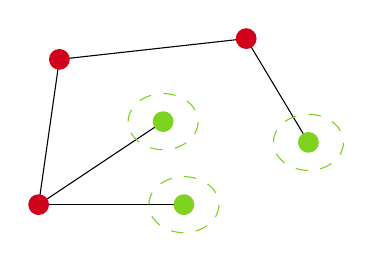
\begin{tikzpicture}[x=0.75pt,y=0.75pt,yscale=-1,xscale=1]
%uncomment if require: \path (0,193); %set diagram left start at 0, and has height of 193

%Straight Lines [id:da0984605927740948] 
\draw    (175,25) -- (165,95) ;
%Straight Lines [id:da6265757458636173] 
\draw    (165,95) -- (235,95) ;
%Straight Lines [id:da12182039563159297] 
\draw    (165,95) -- (225,55) ;
%Straight Lines [id:da667532625992501] 
\draw    (175,25) -- (265,15) ;
%Straight Lines [id:da4994952007175353] 
\draw    (265,15) -- (295,65) ;
%Shape: Circle [id:dp18461176684200264] 
\draw  [draw opacity=0][fill={rgb, 255:red, 208; green, 2; blue, 27 }  ,fill opacity=1 ] (170,25) .. controls (170,22.24) and (172.24,20) .. (175,20) .. controls (177.76,20) and (180,22.24) .. (180,25) .. controls (180,27.76) and (177.76,30) .. (175,30) .. controls (172.24,30) and (170,27.76) .. (170,25) -- cycle ;
%Shape: Circle [id:dp10060882656169834] 
\draw  [draw opacity=0][fill={rgb, 255:red, 208; green, 2; blue, 27 }  ,fill opacity=1 ] (160,95) .. controls (160,92.24) and (162.24,90) .. (165,90) .. controls (167.76,90) and (170,92.24) .. (170,95) .. controls (170,97.76) and (167.76,100) .. (165,100) .. controls (162.24,100) and (160,97.76) .. (160,95) -- cycle ;
%Shape: Circle [id:dp8035247431249818] 
\draw  [draw opacity=0][fill={rgb, 255:red, 208; green, 2; blue, 27 }  ,fill opacity=1 ] (260,15) .. controls (260,12.24) and (262.24,10) .. (265,10) .. controls (267.76,10) and (270,12.24) .. (270,15) .. controls (270,17.76) and (267.76,20) .. (265,20) .. controls (262.24,20) and (260,17.76) .. (260,15) -- cycle ;
%Shape: Circle [id:dp03884028492334557] 
\draw  [draw opacity=0][fill={rgb, 255:red, 126; green, 211; blue, 33 }  ,fill opacity=1 ] (220,55) .. controls (220,52.24) and (222.24,50) .. (225,50) .. controls (227.76,50) and (230,52.24) .. (230,55) .. controls (230,57.76) and (227.76,60) .. (225,60) .. controls (222.24,60) and (220,57.76) .. (220,55) -- cycle ;
%Shape: Circle [id:dp40784864189322] 
\draw  [draw opacity=0][fill={rgb, 255:red, 126; green, 211; blue, 33 }  ,fill opacity=1 ] (290,65) .. controls (290,62.24) and (292.24,60) .. (295,60) .. controls (297.76,60) and (300,62.24) .. (300,65) .. controls (300,67.76) and (297.76,70) .. (295,70) .. controls (292.24,70) and (290,67.76) .. (290,65) -- cycle ;
%Shape: Circle [id:dp034678543816174634] 
\draw  [draw opacity=0][fill={rgb, 255:red, 126; green, 211; blue, 33 }  ,fill opacity=1 ] (230,95) .. controls (230,92.24) and (232.24,90) .. (235,90) .. controls (237.76,90) and (240,92.24) .. (240,95) .. controls (240,97.76) and (237.76,100) .. (235,100) .. controls (232.24,100) and (230,97.76) .. (230,95) -- cycle ;
%Shape: Ellipse [id:dp47417663473871297] 
\draw  [color={rgb, 255:red, 126; green, 211; blue, 33 }  ,draw opacity=1 ][dash pattern={on 4.5pt off 4.5pt}] (208.13,55) .. controls (208.13,47.54) and (215.68,41.5) .. (225,41.5) .. controls (234.32,41.5) and (241.88,47.54) .. (241.88,55) .. controls (241.88,62.46) and (234.32,68.5) .. (225,68.5) .. controls (215.68,68.5) and (208.13,62.46) .. (208.13,55) -- cycle ;
%Shape: Ellipse [id:dp4680354598258094] 
\draw  [color={rgb, 255:red, 126; green, 211; blue, 33 }  ,draw opacity=1 ][dash pattern={on 4.5pt off 4.5pt}] (218.13,95) .. controls (218.13,87.54) and (225.68,81.5) .. (235,81.5) .. controls (244.32,81.5) and (251.88,87.54) .. (251.88,95) .. controls (251.88,102.46) and (244.32,108.5) .. (235,108.5) .. controls (225.68,108.5) and (218.13,102.46) .. (218.13,95) -- cycle ;
%Shape: Ellipse [id:dp7785817672164794] 
\draw  [color={rgb, 255:red, 126; green, 211; blue, 33 }  ,draw opacity=1 ][dash pattern={on 4.5pt off 4.5pt}] (278.13,65) .. controls (278.13,57.54) and (285.68,51.5) .. (295,51.5) .. controls (304.32,51.5) and (311.88,57.54) .. (311.88,65) .. controls (311.88,72.46) and (304.32,78.5) .. (295,78.5) .. controls (285.68,78.5) and (278.13,72.46) .. (278.13,65) -- cycle ;




\end{tikzpicture}

\end{center}
In general, trees has a leaf.

\begin{proposition}[Trees Have Leaves]
	Every tree $T$ with $|T| \geq 2$ has a leaf.
\end{proposition}
\begin{proof}
	Let $T$ be a tree with $|T| \geq 2$, and let $P$ be a path of maximum length in $T$, with $P = x_1 \dots x_k$. We claim that $d(x_k) = 1$. Observe that $\deg(x_k) \geq 1$, since $x_k x_{k - 1} \in E$. If $x_k$ is adjacent to another vertex $y \neq x_{k - 1}$, then either $y \in \{x_1, \dots, x_{k - 2}\}$, which would imply thar $T$ contains a cycle, or $y \not \in \{x_1, \dots, x_{k - 2}\}$, then $x_1 \dots x_k y$ is a path longer than $P$, which violates its maximality.
\end{proof}

\begin{remark}
	This proof gives us two leaves in $T$, which is the best we can hope for considering $P_n$ is a tree with exactly two leaves.
\end{remark}

\begin{proposition}[Edges of a Tree]
	Let $T$ be a tree. Then $e(T) = |T| - 1$.
\end{proposition}
\begin{proof}
	We will do induction on $n = |T|$. If $n = 1$, this is trivial as there is only one edge. Now given $T$ with at least 2 vertices, let $x$ be a leaf in $T$, and define $T' = T - x$.
	
	$T'$ must be acyclic, since we have only removed vertices. $T'$ must also be connected since for all $u, v \in V(T')$ there exists a path from $u$ to $v$ in $T$ that does not use $x$, so it is also a path from $u$ to $v$ in $T'$. Thus $T'$ is a tree.
	Thus by induction, $T'$ has $n - 2$ edges, and $e(T) = e(T') + 1 = |T| - 1$. 
\end{proof}

Now lets think about trees as subgraphs of other graphs.

\begin{definition}[Spanning Tree]
	Let $G$ be a graph. We say $T$ is a \vocab{spanning tree} of $G$ if $T$ is a tree on $V(G)$ and is a subgraph of $G$.
\end{definition}

\begin{center}
	

\tikzset{every picture/.style={line width=0.75pt}} %set default line width to 0.75pt        

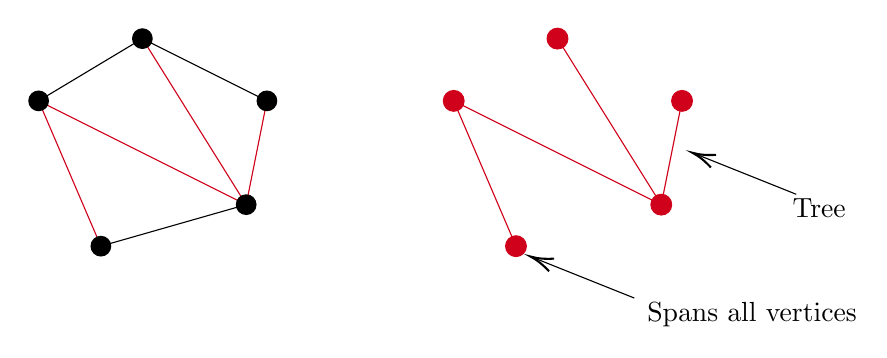
\begin{tikzpicture}[x=0.75pt,y=0.75pt,yscale=-1,xscale=1]
%uncomment if require: \path (0,193); %set diagram left start at 0, and has height of 193

%Straight Lines [id:da7720717972243504] 
\draw    (195,15) -- (145,45) ;
%Straight Lines [id:da7920300217957735] 
\draw [color={rgb, 255:red, 208; green, 2; blue, 27 }  ,draw opacity=1 ]   (175,115) -- (145,45) ;
%Straight Lines [id:da20392691285127829] 
\draw    (175,115) -- (245,95) ;
%Straight Lines [id:da8350342542026185] 
\draw [color={rgb, 255:red, 208; green, 2; blue, 27 }  ,draw opacity=1 ]   (245,95) -- (255,45) ;
%Straight Lines [id:da9158971334401541] 
\draw    (195,15) -- (255,45) ;
%Straight Lines [id:da18144577006731655] 
\draw [color={rgb, 255:red, 208; green, 2; blue, 27 }  ,draw opacity=1 ]   (195,15) -- (245,95) ;
%Straight Lines [id:da7793007821979472] 
\draw [color={rgb, 255:red, 208; green, 2; blue, 27 }  ,draw opacity=1 ]   (145,45) -- (245,95) ;
%Shape: Circle [id:dp1682506259527774] 
\draw  [draw opacity=0][fill={rgb, 255:red, 0; green, 0; blue, 0 }  ,fill opacity=1 ] (190,15) .. controls (190,12.24) and (192.24,10) .. (195,10) .. controls (197.76,10) and (200,12.24) .. (200,15) .. controls (200,17.76) and (197.76,20) .. (195,20) .. controls (192.24,20) and (190,17.76) .. (190,15) -- cycle ;
%Shape: Circle [id:dp6060797868745955] 
\draw  [draw opacity=0][fill={rgb, 255:red, 0; green, 0; blue, 0 }  ,fill opacity=1 ] (140,45) .. controls (140,42.24) and (142.24,40) .. (145,40) .. controls (147.76,40) and (150,42.24) .. (150,45) .. controls (150,47.76) and (147.76,50) .. (145,50) .. controls (142.24,50) and (140,47.76) .. (140,45) -- cycle ;
%Shape: Circle [id:dp5532360644089358] 
\draw  [draw opacity=0][fill={rgb, 255:red, 0; green, 0; blue, 0 }  ,fill opacity=1 ] (170,115) .. controls (170,112.24) and (172.24,110) .. (175,110) .. controls (177.76,110) and (180,112.24) .. (180,115) .. controls (180,117.76) and (177.76,120) .. (175,120) .. controls (172.24,120) and (170,117.76) .. (170,115) -- cycle ;
%Shape: Circle [id:dp9976784820641885] 
\draw  [draw opacity=0][fill={rgb, 255:red, 0; green, 0; blue, 0 }  ,fill opacity=1 ] (240,95) .. controls (240,92.24) and (242.24,90) .. (245,90) .. controls (247.76,90) and (250,92.24) .. (250,95) .. controls (250,97.76) and (247.76,100) .. (245,100) .. controls (242.24,100) and (240,97.76) .. (240,95) -- cycle ;
%Shape: Circle [id:dp362434366455488] 
\draw  [draw opacity=0][fill={rgb, 255:red, 0; green, 0; blue, 0 }  ,fill opacity=1 ] (250,45) .. controls (250,42.24) and (252.24,40) .. (255,40) .. controls (257.76,40) and (260,42.24) .. (260,45) .. controls (260,47.76) and (257.76,50) .. (255,50) .. controls (252.24,50) and (250,47.76) .. (250,45) -- cycle ;
%Straight Lines [id:da15805292190155373] 
\draw [color={rgb, 255:red, 208; green, 2; blue, 27 }  ,draw opacity=1 ][fill={rgb, 255:red, 208; green, 2; blue, 27 }  ,fill opacity=1 ]   (375,115) -- (345,45) ;
%Straight Lines [id:da8535130805001211] 
\draw [color={rgb, 255:red, 208; green, 2; blue, 27 }  ,draw opacity=1 ][fill={rgb, 255:red, 208; green, 2; blue, 27 }  ,fill opacity=1 ]   (445,95) -- (455,45) ;
%Straight Lines [id:da8314095713427262] 
\draw [color={rgb, 255:red, 208; green, 2; blue, 27 }  ,draw opacity=1 ][fill={rgb, 255:red, 208; green, 2; blue, 27 }  ,fill opacity=1 ]   (395,15) -- (445,95) ;
%Straight Lines [id:da7752162474752384] 
\draw [color={rgb, 255:red, 208; green, 2; blue, 27 }  ,draw opacity=1 ][fill={rgb, 255:red, 208; green, 2; blue, 27 }  ,fill opacity=1 ]   (345,45) -- (445,95) ;
%Shape: Circle [id:dp9210808159738209] 
\draw  [color={rgb, 255:red, 208; green, 2; blue, 27 }  ,draw opacity=1 ][fill={rgb, 255:red, 208; green, 2; blue, 27 }  ,fill opacity=1 ] (390,15) .. controls (390,12.24) and (392.24,10) .. (395,10) .. controls (397.76,10) and (400,12.24) .. (400,15) .. controls (400,17.76) and (397.76,20) .. (395,20) .. controls (392.24,20) and (390,17.76) .. (390,15) -- cycle ;
%Shape: Circle [id:dp3107879115086415] 
\draw  [color={rgb, 255:red, 208; green, 2; blue, 27 }  ,draw opacity=1 ][fill={rgb, 255:red, 208; green, 2; blue, 27 }  ,fill opacity=1 ] (340,45) .. controls (340,42.24) and (342.24,40) .. (345,40) .. controls (347.76,40) and (350,42.24) .. (350,45) .. controls (350,47.76) and (347.76,50) .. (345,50) .. controls (342.24,50) and (340,47.76) .. (340,45) -- cycle ;
%Shape: Circle [id:dp6855923108139758] 
\draw  [color={rgb, 255:red, 208; green, 2; blue, 27 }  ,draw opacity=1 ][fill={rgb, 255:red, 208; green, 2; blue, 27 }  ,fill opacity=1 ] (370,115) .. controls (370,112.24) and (372.24,110) .. (375,110) .. controls (377.76,110) and (380,112.24) .. (380,115) .. controls (380,117.76) and (377.76,120) .. (375,120) .. controls (372.24,120) and (370,117.76) .. (370,115) -- cycle ;
%Shape: Circle [id:dp7351941658035576] 
\draw  [color={rgb, 255:red, 208; green, 2; blue, 27 }  ,draw opacity=1 ][fill={rgb, 255:red, 208; green, 2; blue, 27 }  ,fill opacity=1 ] (440,95) .. controls (440,92.24) and (442.24,90) .. (445,90) .. controls (447.76,90) and (450,92.24) .. (450,95) .. controls (450,97.76) and (447.76,100) .. (445,100) .. controls (442.24,100) and (440,97.76) .. (440,95) -- cycle ;
%Shape: Circle [id:dp33930610746251866] 
\draw  [color={rgb, 255:red, 208; green, 2; blue, 27 }  ,draw opacity=1 ][fill={rgb, 255:red, 208; green, 2; blue, 27 }  ,fill opacity=1 ] (450,45) .. controls (450,42.24) and (452.24,40) .. (455,40) .. controls (457.76,40) and (460,42.24) .. (460,45) .. controls (460,47.76) and (457.76,50) .. (455,50) .. controls (452.24,50) and (450,47.76) .. (450,45) -- cycle ;
%Straight Lines [id:da6794496736217942] 
\draw    (510,90) -- (461.86,70.74) ;
\draw [shift={(460,70)}, rotate = 381.8] [color={rgb, 255:red, 0; green, 0; blue, 0 }  ][line width=0.75]    (10.93,-3.29) .. controls (6.95,-1.4) and (3.31,-0.3) .. (0,0) .. controls (3.31,0.3) and (6.95,1.4) .. (10.93,3.29)   ;
%Straight Lines [id:da24613239577970836] 
\draw    (432,140) -- (383.86,120.74) ;
\draw [shift={(382,120)}, rotate = 381.8] [color={rgb, 255:red, 0; green, 0; blue, 0 }  ][line width=0.75]    (10.93,-3.29) .. controls (6.95,-1.4) and (3.31,-0.3) .. (0,0) .. controls (3.31,0.3) and (6.95,1.4) .. (10.93,3.29)   ;

% Text Node
\draw (507,91) node [anchor=north west][inner sep=0.75pt]   [align=left] {Tree};
% Text Node
\draw (437,141) node [anchor=north west][inner sep=0.75pt]   [align=left] {Spans all vertices};


\end{tikzpicture}

\end{center}

Spanning trees are useful in a number of contexts, one of which is giving a sensible ordering to the vertices of a graph. They are particularly useful because of the following result.

\begin{proposition}[Connected Graphs have Spanning Trees]
	Every connected graph contains a spanning tree.
\end{proposition}
\begin{proof}
	A tree is a minimal connected graph. So take the connected graph and remove edges until it becomes a minimal connected graph. Then this will be a subgraph of the original graph, and will thus be a spanning tree.
\end{proof}

\subsection{Bipartite Graphs}

The next type of graph we will look at is \emph{bipartite} graphs.

\begin{definition}[Bipartite Graphs]
	A graph $G = (V, E)$ is \vocab{bipartite} if $V = A \cup B$ where $A \cap B = \emptyset$ and all edges $xy \in E$ have either $x \in A, y \in B$ or $x \in B, y \in A$.
\end{definition}

\begin{example}[Example of Bipartite Graphs]
	The graph below is bipartite, with vertices in the set $A$ being coloured red and vertices in the set $B$ being coloured blue.
	\begin{center}
		

\tikzset{every picture/.style={line width=0.75pt}} %set default line width to 0.75pt        

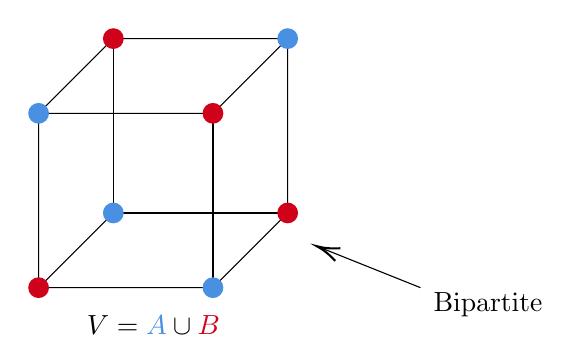
\begin{tikzpicture}[x=0.75pt,y=0.75pt,yscale=-1,xscale=1]
%uncomment if require: \path (0,193); %set diagram left start at 0, and has height of 193

%Straight Lines [id:da6060270401424458] 
\draw    (216,40) -- (216,124) ;
%Straight Lines [id:da23724217319822305] 
\draw    (300,124) -- (216,124) ;
%Straight Lines [id:da19809780044648873] 
\draw    (180,160) -- (216,124) ;
%Straight Lines [id:da24613239577970836] 
\draw    (364,160) -- (315.86,140.74) ;
\draw [shift={(314,140)}, rotate = 381.8] [color={rgb, 255:red, 0; green, 0; blue, 0 }  ][line width=0.75]    (10.93,-3.29) .. controls (6.95,-1.4) and (3.31,-0.3) .. (0,0) .. controls (3.31,0.3) and (6.95,1.4) .. (10.93,3.29)   ;
%Shape: Cube [id:dp9216272317281227] 
\draw   (180,76) -- (216,40) -- (300,40) -- (300,124) -- (264,160) -- (180,160) -- cycle ; \draw   (300,40) -- (264,76) -- (180,76) ; \draw   (264,76) -- (264,160) ;
%Shape: Circle [id:dp7313331826223877] 
\draw  [draw opacity=0][fill={rgb, 255:red, 208; green, 2; blue, 27 }  ,fill opacity=1 ] (175,160) .. controls (175,157.24) and (177.24,155) .. (180,155) .. controls (182.76,155) and (185,157.24) .. (185,160) .. controls (185,162.76) and (182.76,165) .. (180,165) .. controls (177.24,165) and (175,162.76) .. (175,160) -- cycle ;
%Shape: Circle [id:dp9469737817920821] 
\draw  [draw opacity=0][fill={rgb, 255:red, 74; green, 144; blue, 226 }  ,fill opacity=1 ] (259,160) .. controls (259,157.24) and (261.24,155) .. (264,155) .. controls (266.76,155) and (269,157.24) .. (269,160) .. controls (269,162.76) and (266.76,165) .. (264,165) .. controls (261.24,165) and (259,162.76) .. (259,160) -- cycle ;
%Shape: Circle [id:dp927144427433717] 
\draw  [draw opacity=0][fill={rgb, 255:red, 208; green, 2; blue, 27 }  ,fill opacity=1 ] (295,124) .. controls (295,121.24) and (297.24,119) .. (300,119) .. controls (302.76,119) and (305,121.24) .. (305,124) .. controls (305,126.76) and (302.76,129) .. (300,129) .. controls (297.24,129) and (295,126.76) .. (295,124) -- cycle ;
%Shape: Circle [id:dp6195253711881875] 
\draw  [draw opacity=0][fill={rgb, 255:red, 74; green, 144; blue, 226 }  ,fill opacity=1 ] (295,40) .. controls (295,37.24) and (297.24,35) .. (300,35) .. controls (302.76,35) and (305,37.24) .. (305,40) .. controls (305,42.76) and (302.76,45) .. (300,45) .. controls (297.24,45) and (295,42.76) .. (295,40) -- cycle ;
%Shape: Circle [id:dp5745873981618578] 
\draw  [draw opacity=0][fill={rgb, 255:red, 208; green, 2; blue, 27 }  ,fill opacity=1 ] (259,76) .. controls (259,73.24) and (261.24,71) .. (264,71) .. controls (266.76,71) and (269,73.24) .. (269,76) .. controls (269,78.76) and (266.76,81) .. (264,81) .. controls (261.24,81) and (259,78.76) .. (259,76) -- cycle ;
%Shape: Circle [id:dp0848509986260515] 
\draw  [draw opacity=0][fill={rgb, 255:red, 74; green, 144; blue, 226 }  ,fill opacity=1 ] (175,76) .. controls (175,73.24) and (177.24,71) .. (180,71) .. controls (182.76,71) and (185,73.24) .. (185,76) .. controls (185,78.76) and (182.76,81) .. (180,81) .. controls (177.24,81) and (175,78.76) .. (175,76) -- cycle ;
%Shape: Circle [id:dp5237597618279684] 
\draw  [draw opacity=0][fill={rgb, 255:red, 208; green, 2; blue, 27 }  ,fill opacity=1 ] (211,40) .. controls (211,37.24) and (213.24,35) .. (216,35) .. controls (218.76,35) and (221,37.24) .. (221,40) .. controls (221,42.76) and (218.76,45) .. (216,45) .. controls (213.24,45) and (211,42.76) .. (211,40) -- cycle ;
%Shape: Circle [id:dp7456524979791003] 
\draw  [draw opacity=0][fill={rgb, 255:red, 74; green, 144; blue, 226 }  ,fill opacity=1 ] (211,124) .. controls (211,121.24) and (213.24,119) .. (216,119) .. controls (218.76,119) and (221,121.24) .. (221,124) .. controls (221,126.76) and (218.76,129) .. (216,129) .. controls (213.24,129) and (211,126.76) .. (211,124) -- cycle ;

% Text Node
\draw (369,161) node [anchor=north west][inner sep=0.75pt]   [align=left] {Bipartite};
% Text Node
\draw (202,172) node [anchor=north west][inner sep=0.75pt]    {$V=\textcolor[rgb]{0.29,0.56,0.89}{A} \cup \textcolor[rgb]{0.82,0.01,0.11}{B}$};


\end{tikzpicture}

	\end{center}

	An example of a non-bipartite graph is $C_5$. To see this, we can start by choosing a vertex to be in $A$ (without loss of generality), then the adjacent vertices must be in $B$, but then their adjacent vertices must be in $A$, but then there is an edge between two vertices in $A$. This is shown below.

	\begin{center}
		

\tikzset{every picture/.style={line width=0.75pt}} %set default line width to 0.75pt        

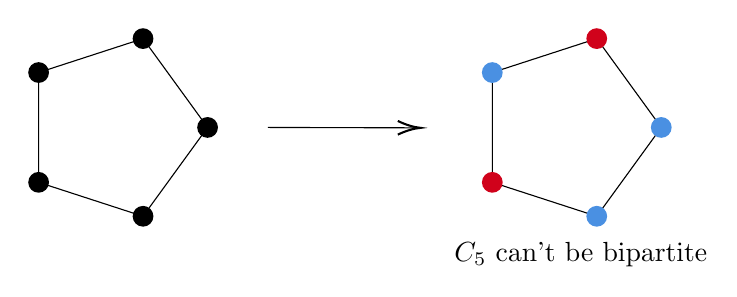
\begin{tikzpicture}[x=0.75pt,y=0.75pt,yscale=-1,xscale=1]
%uncomment if require: \path (0,193); %set diagram left start at 0, and has height of 193

%Shape: Regular Polygon [id:dp6479462597087118] 
\draw   (206.41,87.8) -- (175.31,130.6) -- (125,114.25) -- (125,61.35) -- (175.31,45) -- cycle ;
%Shape: Circle [id:dp9268028209058927] 
\draw  [draw opacity=0][fill={rgb, 255:red, 0; green, 0; blue, 0 }  ,fill opacity=1 ] (201.41,87.8) .. controls (201.41,85.04) and (203.64,82.8) .. (206.41,82.8) .. controls (209.17,82.8) and (211.41,85.04) .. (211.41,87.8) .. controls (211.41,90.56) and (209.17,92.8) .. (206.41,92.8) .. controls (203.64,92.8) and (201.41,90.56) .. (201.41,87.8) -- cycle ;
%Shape: Circle [id:dp5164482643400302] 
\draw  [draw opacity=0][fill={rgb, 255:red, 0; green, 0; blue, 0 }  ,fill opacity=1 ] (170.31,45) .. controls (170.31,42.24) and (172.55,40) .. (175.31,40) .. controls (178.07,40) and (180.31,42.24) .. (180.31,45) .. controls (180.31,47.76) and (178.07,50) .. (175.31,50) .. controls (172.55,50) and (170.31,47.76) .. (170.31,45) -- cycle ;
%Shape: Circle [id:dp6340446217566587] 
\draw  [draw opacity=0][fill={rgb, 255:red, 0; green, 0; blue, 0 }  ,fill opacity=1 ] (120,61.35) .. controls (120,58.59) and (122.24,56.35) .. (125,56.35) .. controls (127.76,56.35) and (130,58.59) .. (130,61.35) .. controls (130,64.11) and (127.76,66.35) .. (125,66.35) .. controls (122.24,66.35) and (120,64.11) .. (120,61.35) -- cycle ;
%Shape: Circle [id:dp6354510885840486] 
\draw  [draw opacity=0][fill={rgb, 255:red, 0; green, 0; blue, 0 }  ,fill opacity=1 ] (120,114.25) .. controls (120,111.49) and (122.24,109.25) .. (125,109.25) .. controls (127.76,109.25) and (130,111.49) .. (130,114.25) .. controls (130,117.01) and (127.76,119.25) .. (125,119.25) .. controls (122.24,119.25) and (120,117.01) .. (120,114.25) -- cycle ;
%Shape: Circle [id:dp7177331645001392] 
\draw  [draw opacity=0][fill={rgb, 255:red, 0; green, 0; blue, 0 }  ,fill opacity=1 ] (170.31,130.6) .. controls (170.31,127.83) and (172.55,125.6) .. (175.31,125.6) .. controls (178.07,125.6) and (180.31,127.83) .. (180.31,130.6) .. controls (180.31,133.36) and (178.07,135.6) .. (175.31,135.6) .. controls (172.55,135.6) and (170.31,133.36) .. (170.31,130.6) -- cycle ;
%Straight Lines [id:da044616960583838905] 
\draw    (235.41,87.8) -- (307,87.99) ;
\draw [shift={(309,88)}, rotate = 180.16] [color={rgb, 255:red, 0; green, 0; blue, 0 }  ][line width=0.75]    (10.93,-3.29) .. controls (6.95,-1.4) and (3.31,-0.3) .. (0,0) .. controls (3.31,0.3) and (6.95,1.4) .. (10.93,3.29)   ;
%Shape: Regular Polygon [id:dp6720141486992529] 
\draw   (425,87.8) -- (393.91,130.6) -- (343.59,114.25) -- (343.59,61.35) -- (393.91,45) -- cycle ;
%Shape: Circle [id:dp6878881253571169] 
\draw  [draw opacity=0][fill={rgb, 255:red, 74; green, 144; blue, 226 }  ,fill opacity=1 ] (420,87.8) .. controls (420,85.04) and (422.24,82.8) .. (425,82.8) .. controls (427.76,82.8) and (430,85.04) .. (430,87.8) .. controls (430,90.56) and (427.76,92.8) .. (425,92.8) .. controls (422.24,92.8) and (420,90.56) .. (420,87.8) -- cycle ;
%Shape: Circle [id:dp7845528979637783] 
\draw  [draw opacity=0][fill={rgb, 255:red, 208; green, 2; blue, 27 }  ,fill opacity=1 ] (388.91,45) .. controls (388.91,42.24) and (391.14,40) .. (393.91,40) .. controls (396.67,40) and (398.91,42.24) .. (398.91,45) .. controls (398.91,47.76) and (396.67,50) .. (393.91,50) .. controls (391.14,50) and (388.91,47.76) .. (388.91,45) -- cycle ;
%Shape: Circle [id:dp35893358645915385] 
\draw  [draw opacity=0][fill={rgb, 255:red, 74; green, 144; blue, 226 }  ,fill opacity=1 ] (338.59,61.35) .. controls (338.59,58.59) and (340.83,56.35) .. (343.59,56.35) .. controls (346.36,56.35) and (348.59,58.59) .. (348.59,61.35) .. controls (348.59,64.11) and (346.36,66.35) .. (343.59,66.35) .. controls (340.83,66.35) and (338.59,64.11) .. (338.59,61.35) -- cycle ;
%Shape: Circle [id:dp814616877870825] 
\draw  [draw opacity=0][fill={rgb, 255:red, 208; green, 2; blue, 27 }  ,fill opacity=1 ] (338.59,114.25) .. controls (338.59,111.49) and (340.83,109.25) .. (343.59,109.25) .. controls (346.36,109.25) and (348.59,111.49) .. (348.59,114.25) .. controls (348.59,117.01) and (346.36,119.25) .. (343.59,119.25) .. controls (340.83,119.25) and (338.59,117.01) .. (338.59,114.25) -- cycle ;
%Shape: Circle [id:dp9973985318086398] 
\draw  [draw opacity=0][fill={rgb, 255:red, 74; green, 144; blue, 226 }  ,fill opacity=1 ] (388.91,130.6) .. controls (388.91,127.83) and (391.14,125.6) .. (393.91,125.6) .. controls (396.67,125.6) and (398.91,127.83) .. (398.91,130.6) .. controls (398.91,133.36) and (396.67,135.6) .. (393.91,135.6) .. controls (391.14,135.6) and (388.91,133.36) .. (388.91,130.6) -- cycle ;

% Text Node
\draw (324,142) node [anchor=north west][inner sep=0.75pt]   [align=left] {$\displaystyle C_{5}$ can't be bipartite};


\end{tikzpicture}

	\end{center}

\end{example}

The argument given for $C_5$ works in general.

\begin{proposition}[Bipartite Cyclic Graphs]
	The cycle $C_{2k + 1}$ is \emph{not} bipartite, and the cycle $C_{2k}$ \emph{is} bipartite.
\end{proposition}
\begin{proof}
	Assume that $C_{2k + 1}$ is bipartite. Then there must be disjoint sets $A$ and $B$, and as $2k + 1$ is odd, we must have (without loss of generality), $|A| > |B|$. Now let's count the edges between $A$ and $B$. This must be $2|A|$ and also $2|B|$, as every vertex has degree 2. But then $|A| = |B|$, which is a contradiction.

	For $C_{2n}$, we can let $v_i \in A$ if $i$ is even and $v_i \in B$ if $i$ is odd. Then a vertex $i$ only has edges to vertices $i - 1$ and $i + 1 \pmod{2}$, which have opposite parity. Thus all edges are between $A$ and $B$, as required.
\end{proof}

There is then a natural question: given some arbitrary graph $G$, how do we determine if a given graph is bipartite? It turns out that there is a nice check for `bipartness'. We will state the result and then do some setup before we prove it. 

\begin{proposition}[Bipartite Criterion]
	A graph $G$ is bipartite if and only if $G$ contains no odd cycles.
\end{proposition}

We need to first develop some theory regarding \emph{circuits}.
Informally, a circuit is like a cycle where we can revisit vertices.


\begin{definition}[Circuit]
A circuit is a sequence $x_1 \dots x_l$ where $x_1 = x_l$ and $x_i x_{i + 1} \in E$. The \vocab{length} of the circuit is $l - 1$, the number of edges traversed in the circuit.
\end{definition}

\begin{definition}[Odd Circuits]
	If the length of a circuit is odd, then we say it is an \vocab{odd circuit}.
\end{definition}

\begin{proposition}
An odd circuit contains an odd cycle.	
\end{proposition}
\begin{proof}
	We will prove this by induction on the length of the circuit. For a circuit of length $3$, the circuit must be a cycle.
	In general, let $C = x_1 \dots x_l$ be our circuit. If $x_1, \dots, x_{l - 1}$ are distinct, then $C$ is a cycle and we are done. 
	
	Otherwise, there exists some $z \in C$ that is repeated. We write 
	$$C = x_1 \dots x_a z x_{a + 2} \dots x_{b} z x_{b + 2} \dots x_l.$$
	We define $C' = x_1 \dots x_a z x_{b + 2} \dots x_l$ and $C'' = z x_{a + 2} \dots x_b z$. The length of $C'$ and $C''$ is strictly less than the length of $C$. One of these circuits must have odd length, and by induction that odd circuit contains an odd cycle.
\end{proof}

We can now prove our original bipartness criterion, that a graph is bipartite if and only if it contains no odd cycles.

\begin{proof}[Proof (Bipartite Criterion)]
	If $G$ was bipartite and contained an odd cycle, then there exists an odd cycle that is bipartite. But this is a contradiction.

	Now if $G$ is not bipartite, we can induct on the number of vertices. For $|G| = 1$, this holds. Now if $G$ is not connected, let $C_1, \dots, C_k$ be the components of $G$. We may now apply our induction to each component of $G$ to obtain a bipartition $V(C_i) = A_i \cup B_i$ for each $i \in 1, \dots, k$. Then $A = A_1 \cup \dots A_k$ and $B = B_1 \cup B_k$ is a bipartition for the whole graph. 
	
	We may now assume without loss of generality that $G$ is connected. Fix some vertex $v \in V$, and define 
	\begin{align*}
		A &= \{u \in V \mid d(u, v) \text{ is odd} \} \\
		B &=  \{u \in V \mid d(u, v) \text{ is even} \}
	\end{align*}
	We claim that $A \cup B$ is a bipartition.

	Assume (for a contradiction) that $u_1$ is adjacent to $u_2$ and $d(u_1, v) \cong d(u_2, v) \pmod{2}$. Then there exists paths $P_1$ from $v$ to $u_1$ and $P_2$ from $u_2$ to $v$ with $|P_1| \equiv |P_2|$. But this implies that $vP_1u_1 u_2 P_2$ defines a odd circuit in $G$. Therefore, by our previous proposition, $G$ contains an odd cycle, which is a contradiction. 
\end{proof}
% Looking back at $k$-regular graphs, we are going to introduce some definitions.

\section{Hall's Theorem}

In this section, we will build up our knowledge of \emph{matchings} so that we can prove the first theorem of the course -- Hall's theorem.

\subsection{Matchings}

An appropriate place to start is probably by defining what a matching is.

\begin{definition}[Matching]
	A \vocab{matching} of $G$ is a collection of edges $M \subseteq E$ so that $\forall e_1, e_2 \in M$ with $e_1 \neq e_2$ has $e_1 \cap e_2 = \emptyset$.
\end{definition}

\begin{center}
	

\tikzset{every picture/.style={line width=0.75pt}} %set default line width to 0.75pt        

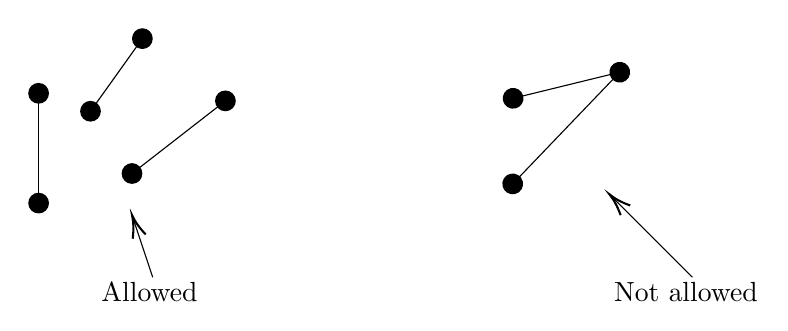
\begin{tikzpicture}[x=0.75pt,y=0.75pt,yscale=-1,xscale=1]
%uncomment if require: \path (0,193); %set diagram left start at 0, and has height of 193

%Shape: Circle [id:dp6340446217566587] 
\draw  [draw opacity=0][fill={rgb, 255:red, 0; green, 0; blue, 0 }  ,fill opacity=1 ] (120,61.35) .. controls (120,58.59) and (122.24,56.35) .. (125,56.35) .. controls (127.76,56.35) and (130,58.59) .. (130,61.35) .. controls (130,64.11) and (127.76,66.35) .. (125,66.35) .. controls (122.24,66.35) and (120,64.11) .. (120,61.35) -- cycle ;
%Shape: Circle [id:dp6354510885840486] 
\draw  [draw opacity=0][fill={rgb, 255:red, 0; green, 0; blue, 0 }  ,fill opacity=1 ] (120,114.25) .. controls (120,111.49) and (122.24,109.25) .. (125,109.25) .. controls (127.76,109.25) and (130,111.49) .. (130,114.25) .. controls (130,117.01) and (127.76,119.25) .. (125,119.25) .. controls (122.24,119.25) and (120,117.01) .. (120,114.25) -- cycle ;
%Straight Lines [id:da9660545408645501] 
\draw    (125,61.35) -- (125,114.25) ;
%Shape: Circle [id:dp07371359600393312] 
\draw  [draw opacity=0][fill={rgb, 255:red, 0; green, 0; blue, 0 }  ,fill opacity=1 ] (170,35) .. controls (170,32.24) and (172.24,30) .. (175,30) .. controls (177.76,30) and (180,32.24) .. (180,35) .. controls (180,37.76) and (177.76,40) .. (175,40) .. controls (172.24,40) and (170,37.76) .. (170,35) -- cycle ;
%Shape: Circle [id:dp7298704478232834] 
\draw  [draw opacity=0][fill={rgb, 255:red, 0; green, 0; blue, 0 }  ,fill opacity=1 ] (145,70) .. controls (145,67.24) and (147.24,65) .. (150,65) .. controls (152.76,65) and (155,67.24) .. (155,70) .. controls (155,72.76) and (152.76,75) .. (150,75) .. controls (147.24,75) and (145,72.76) .. (145,70) -- cycle ;
%Straight Lines [id:da7189218910738701] 
\draw    (175,35) -- (150,70) ;
%Shape: Circle [id:dp2883327905774512] 
\draw  [draw opacity=0][fill={rgb, 255:red, 0; green, 0; blue, 0 }  ,fill opacity=1 ] (165,100) .. controls (165,97.24) and (167.24,95) .. (170,95) .. controls (172.76,95) and (175,97.24) .. (175,100) .. controls (175,102.76) and (172.76,105) .. (170,105) .. controls (167.24,105) and (165,102.76) .. (165,100) -- cycle ;
%Shape: Circle [id:dp895782424476154] 
\draw  [draw opacity=0][fill={rgb, 255:red, 0; green, 0; blue, 0 }  ,fill opacity=1 ] (210,65) .. controls (210,62.24) and (212.24,60) .. (215,60) .. controls (217.76,60) and (220,62.24) .. (220,65) .. controls (220,67.76) and (217.76,70) .. (215,70) .. controls (212.24,70) and (210,67.76) .. (210,65) -- cycle ;
%Straight Lines [id:da41020563458187653] 
\draw    (170,100) -- (215,65) ;
%Shape: Circle [id:dp3162158662674279] 
\draw  [draw opacity=0][fill={rgb, 255:red, 0; green, 0; blue, 0 }  ,fill opacity=1 ] (403.81,46.34) .. controls (406.49,45.68) and (409.2,47.32) .. (409.86,50.01) .. controls (410.51,52.69) and (408.87,55.39) .. (406.19,56.05) .. controls (403.5,56.71) and (400.8,55.07) .. (400.14,52.38) .. controls (399.49,49.7) and (401.13,46.99) .. (403.81,46.34) -- cycle ;
%Shape: Circle [id:dp9128286694228138] 
\draw  [draw opacity=0][fill={rgb, 255:red, 0; green, 0; blue, 0 }  ,fill opacity=1 ] (352.43,58.91) .. controls (355.11,58.26) and (357.81,59.9) .. (358.47,62.58) .. controls (359.13,65.26) and (357.48,67.97) .. (354.8,68.63) .. controls (352.12,69.28) and (349.41,67.64) .. (348.76,64.96) .. controls (348.1,62.27) and (349.74,59.57) .. (352.43,58.91) -- cycle ;
%Straight Lines [id:da7665473567986095] 
\draw    (405,51.19) -- (353.61,63.77) ;
%Shape: Circle [id:dp3935047864716522] 
\draw  [draw opacity=0][fill={rgb, 255:red, 0; green, 0; blue, 0 }  ,fill opacity=1 ] (352.22,100.14) .. controls (354.9,99.49) and (357.61,101.13) .. (358.26,103.81) .. controls (358.92,106.49) and (357.28,109.2) .. (354.6,109.86) .. controls (351.91,110.51) and (349.21,108.87) .. (348.55,106.19) .. controls (347.9,103.5) and (349.54,100.8) .. (352.22,100.14) -- cycle ;
%Straight Lines [id:da4625514392127944] 
\draw    (405,51.19) -- (353.41,105) ;
%Straight Lines [id:da12607406579399916] 
\draw    (180,150) -- (170.63,121.9) ;
\draw [shift={(170,120)}, rotate = 431.57] [color={rgb, 255:red, 0; green, 0; blue, 0 }  ][line width=0.75]    (10.93,-3.29) .. controls (6.95,-1.4) and (3.31,-0.3) .. (0,0) .. controls (3.31,0.3) and (6.95,1.4) .. (10.93,3.29)   ;
%Straight Lines [id:da3703285294357822] 
\draw    (440,150) -- (401.41,111.41) ;
\draw [shift={(400,110)}, rotate = 405] [color={rgb, 255:red, 0; green, 0; blue, 0 }  ][line width=0.75]    (10.93,-3.29) .. controls (6.95,-1.4) and (3.31,-0.3) .. (0,0) .. controls (3.31,0.3) and (6.95,1.4) .. (10.93,3.29)   ;

% Text Node
\draw (154,151) node [anchor=north west][inner sep=0.75pt]   [align=left] {Allowed};
% Text Node
\draw (401,151) node [anchor=north west][inner sep=0.75pt]   [align=left] {Not allowed};


\end{tikzpicture}

\end{center}

\begin{definition}[Saturated]
	Given a graph $G = (V, E)$ and a matching $M$ in $G$, we say that a vertex $v \in V$ is \vocab{saturated by $M$} if there exists an edge in $M$ containing $v$. 
\end{definition}

\begin{center}
	

\tikzset{every picture/.style={line width=0.75pt}} %set default line width to 0.75pt        

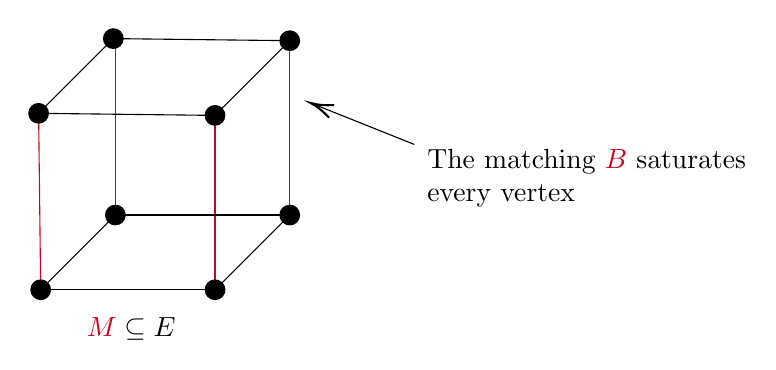
\begin{tikzpicture}[x=0.75pt,y=0.75pt,yscale=-1,xscale=1]
%uncomment if require: \path (0,193); %set diagram left start at 0, and has height of 193

%Straight Lines [id:da805561755073776] 
\draw [color={rgb, 255:red, 208; green, 2; blue, 27 }  ,draw opacity=1 ]   (216,40) -- (216,124) ;
%Straight Lines [id:da4603353852817845] 
\draw [color={rgb, 255:red, 208; green, 2; blue, 27 }  ,draw opacity=1 ]   (264,76) -- (264,160) ;
%Straight Lines [id:da9593359618444844] 
\draw [color={rgb, 255:red, 208; green, 2; blue, 27 }  ,draw opacity=1 ]   (300,40) -- (300,124) ;
%Straight Lines [id:da9136430441630193] 
\draw [color={rgb, 255:red, 208; green, 2; blue, 27 }  ,draw opacity=1 ]   (180,160) -- (179,75) ;
%Straight Lines [id:da752047043089495] 
\draw    (300,124) -- (216,124) ;
%Straight Lines [id:da6627915769720192] 
\draw    (180,160) -- (216,124) ;
%Straight Lines [id:da7505916838885378] 
\draw    (360,90) -- (311.86,70.74) ;
\draw [shift={(310,70)}, rotate = 381.8] [color={rgb, 255:red, 0; green, 0; blue, 0 }  ][line width=0.75]    (10.93,-3.29) .. controls (6.95,-1.4) and (3.31,-0.3) .. (0,0) .. controls (3.31,0.3) and (6.95,1.4) .. (10.93,3.29)   ;
%Shape: Circle [id:dp36912951700681307] 
\draw  [draw opacity=0][fill={rgb, 255:red, 0; green, 0; blue, 0 }  ,fill opacity=1 ] (175,160) .. controls (175,157.24) and (177.24,155) .. (180,155) .. controls (182.76,155) and (185,157.24) .. (185,160) .. controls (185,162.76) and (182.76,165) .. (180,165) .. controls (177.24,165) and (175,162.76) .. (175,160) -- cycle ;
%Shape: Circle [id:dp4704505241972967] 
\draw  [draw opacity=0][fill={rgb, 255:red, 0; green, 0; blue, 0 }  ,fill opacity=1 ] (259,160) .. controls (259,157.24) and (261.24,155) .. (264,155) .. controls (266.76,155) and (269,157.24) .. (269,160) .. controls (269,162.76) and (266.76,165) .. (264,165) .. controls (261.24,165) and (259,162.76) .. (259,160) -- cycle ;
%Shape: Circle [id:dp573647341731309] 
\draw  [draw opacity=0][fill={rgb, 255:red, 0; green, 0; blue, 0 }  ,fill opacity=1 ] (295,124) .. controls (295,121.24) and (297.24,119) .. (300,119) .. controls (302.76,119) and (305,121.24) .. (305,124) .. controls (305,126.76) and (302.76,129) .. (300,129) .. controls (297.24,129) and (295,126.76) .. (295,124) -- cycle ;
%Shape: Circle [id:dp3326458532855674] 
\draw  [draw opacity=0][fill={rgb, 255:red, 0; green, 0; blue, 0 }  ,fill opacity=1 ] (295,40) .. controls (295,37.24) and (297.24,35) .. (300,35) .. controls (302.76,35) and (305,37.24) .. (305,40) .. controls (305,42.76) and (302.76,45) .. (300,45) .. controls (297.24,45) and (295,42.76) .. (295,40) -- cycle ;
%Shape: Circle [id:dp4656041977513993] 
\draw  [draw opacity=0][fill={rgb, 255:red, 0; green, 0; blue, 0 }  ,fill opacity=1 ] (259,76) .. controls (259,73.24) and (261.24,71) .. (264,71) .. controls (266.76,71) and (269,73.24) .. (269,76) .. controls (269,78.76) and (266.76,81) .. (264,81) .. controls (261.24,81) and (259,78.76) .. (259,76) -- cycle ;
%Shape: Circle [id:dp7403175942898133] 
\draw  [draw opacity=0][fill={rgb, 255:red, 0; green, 0; blue, 0 }  ,fill opacity=1 ] (174,75) .. controls (174,72.24) and (176.24,70) .. (179,70) .. controls (181.76,70) and (184,72.24) .. (184,75) .. controls (184,77.76) and (181.76,80) .. (179,80) .. controls (176.24,80) and (174,77.76) .. (174,75) -- cycle ;
%Shape: Circle [id:dp3797103652507142] 
\draw  [draw opacity=0][fill={rgb, 255:red, 0; green, 0; blue, 0 }  ,fill opacity=1 ] (210,39) .. controls (210,36.24) and (212.24,34) .. (215,34) .. controls (217.76,34) and (220,36.24) .. (220,39) .. controls (220,41.76) and (217.76,44) .. (215,44) .. controls (212.24,44) and (210,41.76) .. (210,39) -- cycle ;
%Shape: Circle [id:dp5362787773800174] 
\draw  [draw opacity=0][fill={rgb, 255:red, 0; green, 0; blue, 0 }  ,fill opacity=1 ] (211,124) .. controls (211,121.24) and (213.24,119) .. (216,119) .. controls (218.76,119) and (221,121.24) .. (221,124) .. controls (221,126.76) and (218.76,129) .. (216,129) .. controls (213.24,129) and (211,126.76) .. (211,124) -- cycle ;
%Straight Lines [id:da2121231673256675] 
\draw    (215,39) -- (300,40) ;
%Straight Lines [id:da050391166938102305] 
\draw    (179,75) -- (264,76) ;
%Straight Lines [id:da7012868164712192] 
\draw    (180,160) -- (264,160) ;
%Straight Lines [id:da14338113639691086] 
\draw    (264,160) -- (300,124) ;
%Straight Lines [id:da8236516522079884] 
\draw    (179,75) -- (215,39) ;
%Straight Lines [id:da3281665392341566] 
\draw    (264,76) -- (300,40) ;

% Text Node
\draw (365,91) node [anchor=north west][inner sep=0.75pt]   [align=left] {The matching $\displaystyle \textcolor[rgb]{0.82,0.01,0.11}{B}$ saturates\\every vertex};
% Text Node
\draw (201,172) node [anchor=north west][inner sep=0.75pt]    {$\textcolor[rgb]{0.82,0.01,0.11}{M} \subseteq E$};


\end{tikzpicture}

\end{center}
A matching where every vertex is saturated (such as the above) is known as a \vocab{perfect matching}. However, there is no restriction in general on how many vertices are saturated by a matching.

\subsection{Matching in Bipartite Graphs}

Matchings are particularly interesting in bipartite graphs. We will be interested in the following question: given a bipartite graph $G = (A \cup B, E)$, when can I find a matching saturating $A$?

\begin{center}
	

\tikzset{every picture/.style={line width=0.75pt}} %set default line width to 0.75pt        

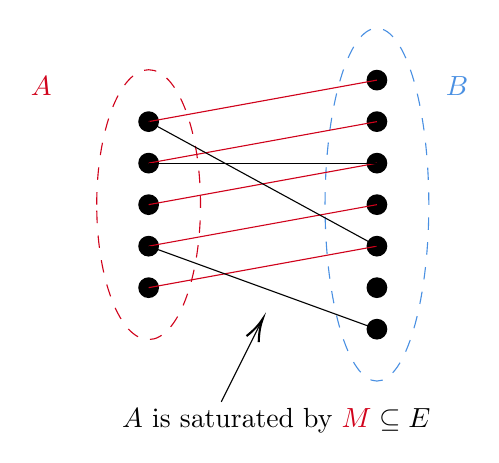
\begin{tikzpicture}[x=0.75pt,y=0.75pt,yscale=-1,xscale=1]
%uncomment if require: \path (0,273); %set diagram left start at 0, and has height of 273

%Straight Lines [id:da7505916838885378] 
\draw    (360,190) -- (379.11,151.79) ;
\draw [shift={(380,150)}, rotate = 476.57] [color={rgb, 255:red, 0; green, 0; blue, 0 }  ][line width=0.75]    (10.93,-3.29) .. controls (6.95,-1.4) and (3.31,-0.3) .. (0,0) .. controls (3.31,0.3) and (6.95,1.4) .. (10.93,3.29)   ;
%Shape: Circle [id:dp36912951700681307] 
\draw  [draw opacity=0][fill={rgb, 255:red, 0; green, 0; blue, 0 }  ,fill opacity=1 ] (320,95) .. controls (320,92.24) and (322.24,90) .. (325,90) .. controls (327.76,90) and (330,92.24) .. (330,95) .. controls (330,97.76) and (327.76,100) .. (325,100) .. controls (322.24,100) and (320,97.76) .. (320,95) -- cycle ;
%Shape: Circle [id:dp44942679974813216] 
\draw  [draw opacity=0][fill={rgb, 255:red, 0; green, 0; blue, 0 }  ,fill opacity=1 ] (320,115) .. controls (320,112.24) and (322.24,110) .. (325,110) .. controls (327.76,110) and (330,112.24) .. (330,115) .. controls (330,117.76) and (327.76,120) .. (325,120) .. controls (322.24,120) and (320,117.76) .. (320,115) -- cycle ;
%Shape: Circle [id:dp6752731223210899] 
\draw  [draw opacity=0][fill={rgb, 255:red, 0; green, 0; blue, 0 }  ,fill opacity=1 ] (320,75) .. controls (320,72.24) and (322.24,70) .. (325,70) .. controls (327.76,70) and (330,72.24) .. (330,75) .. controls (330,77.76) and (327.76,80) .. (325,80) .. controls (322.24,80) and (320,77.76) .. (320,75) -- cycle ;
%Shape: Circle [id:dp4233872987178915] 
\draw  [draw opacity=0][fill={rgb, 255:red, 0; green, 0; blue, 0 }  ,fill opacity=1 ] (320,55) .. controls (320,52.24) and (322.24,50) .. (325,50) .. controls (327.76,50) and (330,52.24) .. (330,55) .. controls (330,57.76) and (327.76,60) .. (325,60) .. controls (322.24,60) and (320,57.76) .. (320,55) -- cycle ;
%Shape: Circle [id:dp04653911603417005] 
\draw  [draw opacity=0][fill={rgb, 255:red, 0; green, 0; blue, 0 }  ,fill opacity=1 ] (320,135) .. controls (320,132.24) and (322.24,130) .. (325,130) .. controls (327.76,130) and (330,132.24) .. (330,135) .. controls (330,137.76) and (327.76,140) .. (325,140) .. controls (322.24,140) and (320,137.76) .. (320,135) -- cycle ;
%Shape: Ellipse [id:dp31141580503923916] 
\draw  [color={rgb, 255:red, 208; green, 2; blue, 27 }  ,draw opacity=1 ][dash pattern={on 4.5pt off 4.5pt}] (300,95) .. controls (300,59.1) and (311.19,30) .. (325,30) .. controls (338.81,30) and (350,59.1) .. (350,95) .. controls (350,130.9) and (338.81,160) .. (325,160) .. controls (311.19,160) and (300,130.9) .. (300,95) -- cycle ;
%Shape: Circle [id:dp6358985628093098] 
\draw  [draw opacity=0][fill={rgb, 255:red, 0; green, 0; blue, 0 }  ,fill opacity=1 ] (430,75) .. controls (430,72.24) and (432.24,70) .. (435,70) .. controls (437.76,70) and (440,72.24) .. (440,75) .. controls (440,77.76) and (437.76,80) .. (435,80) .. controls (432.24,80) and (430,77.76) .. (430,75) -- cycle ;
%Shape: Circle [id:dp880304645428568] 
\draw  [draw opacity=0][fill={rgb, 255:red, 0; green, 0; blue, 0 }  ,fill opacity=1 ] (430,95) .. controls (430,92.24) and (432.24,90) .. (435,90) .. controls (437.76,90) and (440,92.24) .. (440,95) .. controls (440,97.76) and (437.76,100) .. (435,100) .. controls (432.24,100) and (430,97.76) .. (430,95) -- cycle ;
%Shape: Circle [id:dp9506904233850559] 
\draw  [draw opacity=0][fill={rgb, 255:red, 0; green, 0; blue, 0 }  ,fill opacity=1 ] (430,55) .. controls (430,52.24) and (432.24,50) .. (435,50) .. controls (437.76,50) and (440,52.24) .. (440,55) .. controls (440,57.76) and (437.76,60) .. (435,60) .. controls (432.24,60) and (430,57.76) .. (430,55) -- cycle ;
%Shape: Circle [id:dp594682452060607] 
\draw  [draw opacity=0][fill={rgb, 255:red, 0; green, 0; blue, 0 }  ,fill opacity=1 ] (430,35) .. controls (430,32.24) and (432.24,30) .. (435,30) .. controls (437.76,30) and (440,32.24) .. (440,35) .. controls (440,37.76) and (437.76,40) .. (435,40) .. controls (432.24,40) and (430,37.76) .. (430,35) -- cycle ;
%Shape: Circle [id:dp7145369093884492] 
\draw  [draw opacity=0][fill={rgb, 255:red, 0; green, 0; blue, 0 }  ,fill opacity=1 ] (430,115) .. controls (430,112.24) and (432.24,110) .. (435,110) .. controls (437.76,110) and (440,112.24) .. (440,115) .. controls (440,117.76) and (437.76,120) .. (435,120) .. controls (432.24,120) and (430,117.76) .. (430,115) -- cycle ;
%Shape: Ellipse [id:dp7407681681896772] 
\draw  [color={rgb, 255:red, 74; green, 144; blue, 226 }  ,draw opacity=1 ][dash pattern={on 4.5pt off 4.5pt}] (410,95) .. controls (410,48.06) and (421.19,10) .. (435,10) .. controls (448.81,10) and (460,48.06) .. (460,95) .. controls (460,141.94) and (448.81,180) .. (435,180) .. controls (421.19,180) and (410,141.94) .. (410,95) -- cycle ;
%Shape: Circle [id:dp33340512760145824] 
\draw  [draw opacity=0][fill={rgb, 255:red, 0; green, 0; blue, 0 }  ,fill opacity=1 ] (430,135) .. controls (430,132.24) and (432.24,130) .. (435,130) .. controls (437.76,130) and (440,132.24) .. (440,135) .. controls (440,137.76) and (437.76,140) .. (435,140) .. controls (432.24,140) and (430,137.76) .. (430,135) -- cycle ;
%Shape: Circle [id:dp724679030580349] 
\draw  [draw opacity=0][fill={rgb, 255:red, 0; green, 0; blue, 0 }  ,fill opacity=1 ] (430,155) .. controls (430,152.24) and (432.24,150) .. (435,150) .. controls (437.76,150) and (440,152.24) .. (440,155) .. controls (440,157.76) and (437.76,160) .. (435,160) .. controls (432.24,160) and (430,157.76) .. (430,155) -- cycle ;
%Straight Lines [id:da6673725902420062] 
\draw [color={rgb, 255:red, 208; green, 2; blue, 27 }  ,draw opacity=1 ]   (325,55) -- (435,35) ;
%Straight Lines [id:da4203133178921782] 
\draw [color={rgb, 255:red, 208; green, 2; blue, 27 }  ,draw opacity=1 ]   (325,75) -- (435,55) ;
%Straight Lines [id:da16049164399667892] 
\draw [color={rgb, 255:red, 208; green, 2; blue, 27 }  ,draw opacity=1 ]   (325,95) -- (435,75) ;
%Straight Lines [id:da19642811620000844] 
\draw [color={rgb, 255:red, 208; green, 2; blue, 27 }  ,draw opacity=1 ]   (325,115) -- (435,95) ;
%Straight Lines [id:da21466460093090467] 
\draw [color={rgb, 255:red, 208; green, 2; blue, 27 }  ,draw opacity=1 ]   (325,135) -- (435,115) ;
%Straight Lines [id:da04929331633411782] 
\draw    (325,115) -- (435,155) ;
%Straight Lines [id:da7611641968859248] 
\draw    (325,75) -- (435,75) ;
%Straight Lines [id:da5620035391275132] 
\draw    (325,55) -- (435,115) ;

% Text Node
\draw (311,192) node [anchor=north west][inner sep=0.75pt]   [align=left] {$\displaystyle A$ is saturated by $\displaystyle \textcolor[rgb]{0.82,0.01,0.11}{M} \subseteq E$};
% Text Node
\draw (267,32) node [anchor=north west][inner sep=0.75pt]    {$\textcolor[rgb]{0.82,0.01,0.11}{A}$};
% Text Node
\draw (467,32) node [anchor=north west][inner sep=0.75pt]  [color={rgb, 255:red, 74; green, 144; blue, 226 }  ,opacity=1 ]  {$B$};


\end{tikzpicture}
\end{center}

This question is the same as asking when is there a function $f: A \rightarrow B$ where $xf(x) \in E$ that is an injection.

In trying to answer this question, we might try and think about why it may not be possible. The simplest reason is when $B$ isn't large enough to have an injection, when $|B| \leq |A|$. In a similar way, we might have a graph is big enough, but that isn't true for a small part of the graph, like below.
\begin{center}
	

\tikzset{every picture/.style={line width=0.75pt}} %set default line width to 0.75pt        

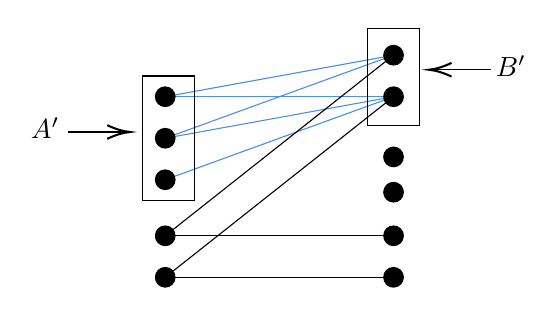
\begin{tikzpicture}[x=0.75pt,y=0.75pt,yscale=-1,xscale=1]
%uncomment if require: \path (0,273); %set diagram left start at 0, and has height of 273

%Straight Lines [id:da8369400892067791] 
\draw    (324,130) -- (434,130) ;
%Straight Lines [id:da19495235143878997] 
\draw    (324,150) -- (434,150) ;
%Straight Lines [id:da40390592166983896] 
\draw [color={rgb, 255:red, 74; green, 144; blue, 226 }  ,draw opacity=1 ]   (324,63) -- (434,43) ;
%Straight Lines [id:da3965802064481285] 
\draw [color={rgb, 255:red, 74; green, 144; blue, 226 }  ,draw opacity=1 ]   (324,83) -- (434,43) ;
%Straight Lines [id:da6637904851386653] 
\draw [color={rgb, 255:red, 74; green, 144; blue, 226 }  ,draw opacity=1 ]   (324,103) -- (434,63) ;
%Straight Lines [id:da1589473171205299] 
\draw [color={rgb, 255:red, 74; green, 144; blue, 226 }  ,draw opacity=1 ]   (324,83) -- (434,63) ;
%Straight Lines [id:da6181500242724567] 
\draw [color={rgb, 255:red, 74; green, 144; blue, 226 }  ,draw opacity=1 ]   (324,63) -- (434,63) ;
%Straight Lines [id:da7181423353650153] 
\draw    (324,130) -- (434,43) ;
%Straight Lines [id:da38882946887707004] 
\draw    (324,150) -- (434,63) ;
%Shape: Circle [id:dp42681003962364517] 
\draw  [draw opacity=0][fill={rgb, 255:red, 0; green, 0; blue, 0 }  ,fill opacity=1 ] (319,103) .. controls (319,100.24) and (321.24,98) .. (324,98) .. controls (326.76,98) and (329,100.24) .. (329,103) .. controls (329,105.76) and (326.76,108) .. (324,108) .. controls (321.24,108) and (319,105.76) .. (319,103) -- cycle ;
%Shape: Circle [id:dp04672707446321711] 
\draw  [draw opacity=0][fill={rgb, 255:red, 0; green, 0; blue, 0 }  ,fill opacity=1 ] (319,130) .. controls (319,127.24) and (321.24,125) .. (324,125) .. controls (326.76,125) and (329,127.24) .. (329,130) .. controls (329,132.76) and (326.76,135) .. (324,135) .. controls (321.24,135) and (319,132.76) .. (319,130) -- cycle ;
%Shape: Circle [id:dp6968869451584372] 
\draw  [draw opacity=0][fill={rgb, 255:red, 0; green, 0; blue, 0 }  ,fill opacity=1 ] (319,83) .. controls (319,80.24) and (321.24,78) .. (324,78) .. controls (326.76,78) and (329,80.24) .. (329,83) .. controls (329,85.76) and (326.76,88) .. (324,88) .. controls (321.24,88) and (319,85.76) .. (319,83) -- cycle ;
%Shape: Circle [id:dp5397070239729519] 
\draw  [draw opacity=0][fill={rgb, 255:red, 0; green, 0; blue, 0 }  ,fill opacity=1 ] (319,63) .. controls (319,60.24) and (321.24,58) .. (324,58) .. controls (326.76,58) and (329,60.24) .. (329,63) .. controls (329,65.76) and (326.76,68) .. (324,68) .. controls (321.24,68) and (319,65.76) .. (319,63) -- cycle ;
%Shape: Circle [id:dp1933015038500212] 
\draw  [draw opacity=0][fill={rgb, 255:red, 0; green, 0; blue, 0 }  ,fill opacity=1 ] (319,150) .. controls (319,147.24) and (321.24,145) .. (324,145) .. controls (326.76,145) and (329,147.24) .. (329,150) .. controls (329,152.76) and (326.76,155) .. (324,155) .. controls (321.24,155) and (319,152.76) .. (319,150) -- cycle ;
%Shape: Circle [id:dp22027602623518294] 
\draw  [draw opacity=0][fill={rgb, 255:red, 0; green, 0; blue, 0 }  ,fill opacity=1 ] (429,92) .. controls (429,89.24) and (431.24,87) .. (434,87) .. controls (436.76,87) and (439,89.24) .. (439,92) .. controls (439,94.76) and (436.76,97) .. (434,97) .. controls (431.24,97) and (429,94.76) .. (429,92) -- cycle ;
%Shape: Circle [id:dp6065822004480979] 
\draw  [draw opacity=0][fill={rgb, 255:red, 0; green, 0; blue, 0 }  ,fill opacity=1 ] (429,109) .. controls (429,106.24) and (431.24,104) .. (434,104) .. controls (436.76,104) and (439,106.24) .. (439,109) .. controls (439,111.76) and (436.76,114) .. (434,114) .. controls (431.24,114) and (429,111.76) .. (429,109) -- cycle ;
%Shape: Circle [id:dp8722990507351452] 
\draw  [draw opacity=0][fill={rgb, 255:red, 0; green, 0; blue, 0 }  ,fill opacity=1 ] (429,63) .. controls (429,60.24) and (431.24,58) .. (434,58) .. controls (436.76,58) and (439,60.24) .. (439,63) .. controls (439,65.76) and (436.76,68) .. (434,68) .. controls (431.24,68) and (429,65.76) .. (429,63) -- cycle ;
%Shape: Circle [id:dp6972009025737637] 
\draw  [draw opacity=0][fill={rgb, 255:red, 0; green, 0; blue, 0 }  ,fill opacity=1 ] (429,43) .. controls (429,40.24) and (431.24,38) .. (434,38) .. controls (436.76,38) and (439,40.24) .. (439,43) .. controls (439,45.76) and (436.76,48) .. (434,48) .. controls (431.24,48) and (429,45.76) .. (429,43) -- cycle ;
%Shape: Circle [id:dp036260952386616085] 
\draw  [draw opacity=0][fill={rgb, 255:red, 0; green, 0; blue, 0 }  ,fill opacity=1 ] (429,130) .. controls (429,127.24) and (431.24,125) .. (434,125) .. controls (436.76,125) and (439,127.24) .. (439,130) .. controls (439,132.76) and (436.76,135) .. (434,135) .. controls (431.24,135) and (429,132.76) .. (429,130) -- cycle ;
%Shape: Circle [id:dp3214854269825461] 
\draw  [draw opacity=0][fill={rgb, 255:red, 0; green, 0; blue, 0 }  ,fill opacity=1 ] (429,150) .. controls (429,147.24) and (431.24,145) .. (434,145) .. controls (436.76,145) and (439,147.24) .. (439,150) .. controls (439,152.76) and (436.76,155) .. (434,155) .. controls (431.24,155) and (429,152.76) .. (429,150) -- cycle ;
%Shape: Rectangle [id:dp8613689383791837] 
\draw   (313,53) -- (338,53) -- (338,113) -- (313,113) -- cycle ;
%Shape: Rectangle [id:dp49091409543282016] 
\draw   (421.5,30) -- (446.5,30) -- (446.5,77) -- (421.5,77) -- cycle ;
%Straight Lines [id:da8087602747586281] 
\draw    (277,80) -- (305,80) ;
\draw [shift={(307,80)}, rotate = 180] [color={rgb, 255:red, 0; green, 0; blue, 0 }  ][line width=0.75]    (10.93,-3.29) .. controls (6.95,-1.4) and (3.31,-0.3) .. (0,0) .. controls (3.31,0.3) and (6.95,1.4) .. (10.93,3.29)   ;
%Straight Lines [id:da9186974784747017] 
\draw    (481,50) -- (453,50) ;
\draw [shift={(451,50)}, rotate = 360] [color={rgb, 255:red, 0; green, 0; blue, 0 }  ][line width=0.75]    (10.93,-3.29) .. controls (6.95,-1.4) and (3.31,-0.3) .. (0,0) .. controls (3.31,0.3) and (6.95,1.4) .. (10.93,3.29)   ;

% Text Node
\draw (258,72) node [anchor=north west][inner sep=0.75pt]    {$A'$};
% Text Node
\draw (482,42) node [anchor=north west][inner sep=0.75pt]    {$B'$};


\end{tikzpicture}

\end{center}
What Hall's theorem says is that this issue is the only obstruction to creating such a matching. 

\begin{definition}[Neighbourhood of a Vertex Set]
	If $X \subseteq V$, then we define $N(X)$, the \vocab{neighbourhood of $X$} to be $\displaystyle N(X) = \bigcup_{x \in X} N(x)$.
\end{definition}

With the notion of the neighborhood of a set of vertices, we can rephrase the issue mentioned about as $|N(A')| < |A'|$ for some subset $A' \subseteq A$. We will use this notation in our statement for Hall's theorem.

Before we prove the theorem, we will need to prepare a little bit.

\begin{definition}[$M$-Alternating Path]
	Let $G = (V, E)$ be a graph with a matching $M$ in $G$. We say that a path $P = x_1 \dots x_l$ is \vocab{M-alternating} if $x_i x_{i + 1}$ is alternately in $M$ and not in $M$.
\end{definition}

\begin{center}
	

\tikzset{every picture/.style={line width=0.75pt}} %set default line width to 0.75pt        

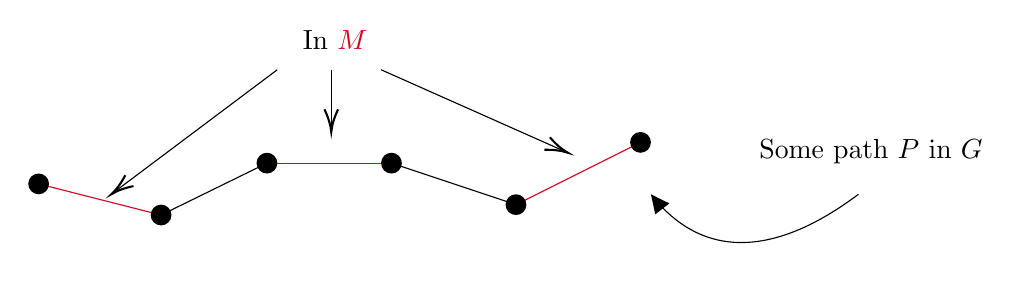
\begin{tikzpicture}[x=0.75pt,y=0.75pt,yscale=-1,xscale=1]
%uncomment if require: \path (0,273); %set diagram left start at 0, and has height of 273

%Straight Lines [id:da1911727766997673] 
\draw    (324,130) -- (375,105) ;
%Straight Lines [id:da41633838448849425] 
\draw [color={rgb, 255:red, 208; green, 2; blue, 27 }  ,draw opacity=1 ]   (375,105) -- (435,105) ;
%Straight Lines [id:da6472416846171128] 
\draw    (435,105) -- (495,125) ;
%Straight Lines [id:da8981575716010599] 
\draw [color={rgb, 255:red, 208; green, 2; blue, 27 }  ,draw opacity=1 ]   (495,125) -- (555,95) ;
%Straight Lines [id:da7701616382388665] 
\draw [color={rgb, 255:red, 208; green, 2; blue, 27 }  ,draw opacity=1 ]   (324,130) -- (265,115) ;
%Shape: Circle [id:dp7703800629553158] 
\draw  [draw opacity=0][fill={rgb, 255:red, 0; green, 0; blue, 0 }  ,fill opacity=1 ] (319,130) .. controls (319,127.24) and (321.24,125) .. (324,125) .. controls (326.76,125) and (329,127.24) .. (329,130) .. controls (329,132.76) and (326.76,135) .. (324,135) .. controls (321.24,135) and (319,132.76) .. (319,130) -- cycle ;
%Shape: Circle [id:dp0226725339534235] 
\draw  [draw opacity=0][fill={rgb, 255:red, 0; green, 0; blue, 0 }  ,fill opacity=1 ] (370,105) .. controls (370,102.24) and (372.24,100) .. (375,100) .. controls (377.76,100) and (380,102.24) .. (380,105) .. controls (380,107.76) and (377.76,110) .. (375,110) .. controls (372.24,110) and (370,107.76) .. (370,105) -- cycle ;
%Shape: Circle [id:dp34568978664728356] 
\draw  [draw opacity=0][fill={rgb, 255:red, 0; green, 0; blue, 0 }  ,fill opacity=1 ] (430,105) .. controls (430,102.24) and (432.24,100) .. (435,100) .. controls (437.76,100) and (440,102.24) .. (440,105) .. controls (440,107.76) and (437.76,110) .. (435,110) .. controls (432.24,110) and (430,107.76) .. (430,105) -- cycle ;
%Shape: Circle [id:dp8179415147207098] 
\draw  [draw opacity=0][fill={rgb, 255:red, 0; green, 0; blue, 0 }  ,fill opacity=1 ] (490,125) .. controls (490,122.24) and (492.24,120) .. (495,120) .. controls (497.76,120) and (500,122.24) .. (500,125) .. controls (500,127.76) and (497.76,130) .. (495,130) .. controls (492.24,130) and (490,127.76) .. (490,125) -- cycle ;
%Shape: Circle [id:dp0812463035943316] 
\draw  [draw opacity=0][fill={rgb, 255:red, 0; green, 0; blue, 0 }  ,fill opacity=1 ] (550,95) .. controls (550,92.24) and (552.24,90) .. (555,90) .. controls (557.76,90) and (560,92.24) .. (560,95) .. controls (560,97.76) and (557.76,100) .. (555,100) .. controls (552.24,100) and (550,97.76) .. (550,95) -- cycle ;
%Shape: Circle [id:dp412793926190299] 
\draw  [draw opacity=0][fill={rgb, 255:red, 0; green, 0; blue, 0 }  ,fill opacity=1 ] (260,115) .. controls (260,112.24) and (262.24,110) .. (265,110) .. controls (267.76,110) and (270,112.24) .. (270,115) .. controls (270,117.76) and (267.76,120) .. (265,120) .. controls (262.24,120) and (260,117.76) .. (260,115) -- cycle ;
%Straight Lines [id:da524865354422517] 
\draw    (380,60) -- (301.6,118.8) ;
\draw [shift={(300,120)}, rotate = 323.13] [color={rgb, 255:red, 0; green, 0; blue, 0 }  ][line width=0.75]    (10.93,-3.29) .. controls (6.95,-1.4) and (3.31,-0.3) .. (0,0) .. controls (3.31,0.3) and (6.95,1.4) .. (10.93,3.29)   ;
%Straight Lines [id:da3699327393316867] 
\draw    (406,60) -- (406,88) ;
\draw [shift={(406,90)}, rotate = 270] [color={rgb, 255:red, 0; green, 0; blue, 0 }  ][line width=0.75]    (10.93,-3.29) .. controls (6.95,-1.4) and (3.31,-0.3) .. (0,0) .. controls (3.31,0.3) and (6.95,1.4) .. (10.93,3.29)   ;
%Straight Lines [id:da39528029770693984] 
\draw    (430,60) -- (518.17,99.19) ;
\draw [shift={(520,100)}, rotate = 203.96] [color={rgb, 255:red, 0; green, 0; blue, 0 }  ][line width=0.75]    (10.93,-3.29) .. controls (6.95,-1.4) and (3.31,-0.3) .. (0,0) .. controls (3.31,0.3) and (6.95,1.4) .. (10.93,3.29)   ;
%Curve Lines [id:da07952038804691897] 
\draw    (561.89,122.34) .. controls (586.75,151.88) and (621,149.25) .. (660,120) ;
\draw [shift={(560,120)}, rotate = 52] [fill={rgb, 255:red, 0; green, 0; blue, 0 }  ][line width=0.08]  [draw opacity=0] (8.93,-4.29) -- (0,0) -- (8.93,4.29) -- cycle    ;

% Text Node
\draw (391,40) node [anchor=north west][inner sep=0.75pt]   [align=left] {In $\displaystyle \textcolor[rgb]{0.82,0.01,0.11}{M}$};
% Text Node
\draw (611,92) node [anchor=north west][inner sep=0.75pt]   [align=left] {Some path $\displaystyle P$ in $\displaystyle G$};


\end{tikzpicture}

\end{center}

Another example of an $M$-alternating path is the one below.
\begin{center}
	

\tikzset{every picture/.style={line width=0.75pt}} %set default line width to 0.75pt        

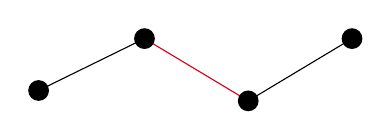
\begin{tikzpicture}[x=0.75pt,y=0.75pt,yscale=-1,xscale=1]
%uncomment if require: \path (0,273); %set diagram left start at 0, and has height of 273

%Straight Lines [id:da6545369317269095] 
\draw    (324,130) -- (375,105) ;
%Straight Lines [id:da5998112575007682] 
\draw [color={rgb, 255:red, 208; green, 2; blue, 27 }  ,draw opacity=1 ]   (375,105) -- (425,135) ;
%Straight Lines [id:da3813029402731277] 
\draw    (425,135) -- (475,105) ;
%Shape: Circle [id:dp4518952685232853] 
\draw  [draw opacity=0][fill={rgb, 255:red, 0; green, 0; blue, 0 }  ,fill opacity=1 ] (319,130) .. controls (319,127.24) and (321.24,125) .. (324,125) .. controls (326.76,125) and (329,127.24) .. (329,130) .. controls (329,132.76) and (326.76,135) .. (324,135) .. controls (321.24,135) and (319,132.76) .. (319,130) -- cycle ;
%Shape: Circle [id:dp4872392702945506] 
\draw  [draw opacity=0][fill={rgb, 255:red, 0; green, 0; blue, 0 }  ,fill opacity=1 ] (370,105) .. controls (370,102.24) and (372.24,100) .. (375,100) .. controls (377.76,100) and (380,102.24) .. (380,105) .. controls (380,107.76) and (377.76,110) .. (375,110) .. controls (372.24,110) and (370,107.76) .. (370,105) -- cycle ;
%Shape: Circle [id:dp8339741130332603] 
\draw  [draw opacity=0][fill={rgb, 255:red, 0; green, 0; blue, 0 }  ,fill opacity=1 ] (420,135) .. controls (420,132.24) and (422.24,130) .. (425,130) .. controls (427.76,130) and (430,132.24) .. (430,135) .. controls (430,137.76) and (427.76,140) .. (425,140) .. controls (422.24,140) and (420,137.76) .. (420,135) -- cycle ;
%Shape: Circle [id:dp6104072071427933] 
\draw  [draw opacity=0][fill={rgb, 255:red, 0; green, 0; blue, 0 }  ,fill opacity=1 ] (470,105) .. controls (470,102.24) and (472.24,100) .. (475,100) .. controls (477.76,100) and (480,102.24) .. (480,105) .. controls (480,107.76) and (477.76,110) .. (475,110) .. controls (472.24,110) and (470,107.76) .. (470,105) -- cycle ;




\end{tikzpicture}

\end{center}
If we saw the path above in the graph, and we knew that the end vertices was not saturated, then we could change the edges that are in $M$, so we would still have a matching. This move will be key in our proof of Hall's theorem.
\begin{center}
	

\tikzset{every picture/.style={line width=0.75pt}} %set default line width to 0.75pt        

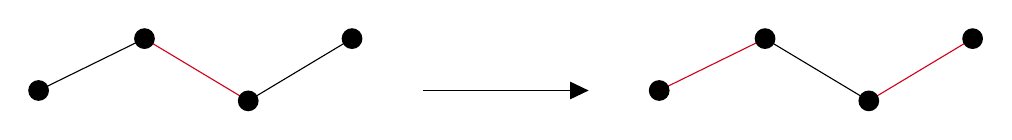
\begin{tikzpicture}[x=0.75pt,y=0.75pt,yscale=-1,xscale=1]
%uncomment if require: \path (0,273); %set diagram left start at 0, and has height of 273

%Straight Lines [id:da8888863291662378] 
\draw    (85,130) -- (136,105) ;
%Straight Lines [id:da2469822147132278] 
\draw [color={rgb, 255:red, 208; green, 2; blue, 27 }  ,draw opacity=1 ]   (136,105) -- (186,135) ;
%Straight Lines [id:da728605608255147] 
\draw    (186,135) -- (236,105) ;
%Shape: Circle [id:dp4177428980499841] 
\draw  [draw opacity=0][fill={rgb, 255:red, 0; green, 0; blue, 0 }  ,fill opacity=1 ] (80,130) .. controls (80,127.24) and (82.24,125) .. (85,125) .. controls (87.76,125) and (90,127.24) .. (90,130) .. controls (90,132.76) and (87.76,135) .. (85,135) .. controls (82.24,135) and (80,132.76) .. (80,130) -- cycle ;
%Shape: Circle [id:dp6460331997754131] 
\draw  [draw opacity=0][fill={rgb, 255:red, 0; green, 0; blue, 0 }  ,fill opacity=1 ] (131,105) .. controls (131,102.24) and (133.24,100) .. (136,100) .. controls (138.76,100) and (141,102.24) .. (141,105) .. controls (141,107.76) and (138.76,110) .. (136,110) .. controls (133.24,110) and (131,107.76) .. (131,105) -- cycle ;
%Shape: Circle [id:dp645196452335059] 
\draw  [draw opacity=0][fill={rgb, 255:red, 0; green, 0; blue, 0 }  ,fill opacity=1 ] (181,135) .. controls (181,132.24) and (183.24,130) .. (186,130) .. controls (188.76,130) and (191,132.24) .. (191,135) .. controls (191,137.76) and (188.76,140) .. (186,140) .. controls (183.24,140) and (181,137.76) .. (181,135) -- cycle ;
%Shape: Circle [id:dp5500348242602249] 
\draw  [draw opacity=0][fill={rgb, 255:red, 0; green, 0; blue, 0 }  ,fill opacity=1 ] (231,105) .. controls (231,102.24) and (233.24,100) .. (236,100) .. controls (238.76,100) and (241,102.24) .. (241,105) .. controls (241,107.76) and (238.76,110) .. (236,110) .. controls (233.24,110) and (231,107.76) .. (231,105) -- cycle ;
%Straight Lines [id:da04862323828569037] 
\draw [color={rgb, 255:red, 208; green, 2; blue, 27 }  ,draw opacity=1 ]   (384,130) -- (435,105) ;
%Straight Lines [id:da8593276291450644] 
\draw [color={rgb, 255:red, 0; green, 0; blue, 0 }  ,draw opacity=1 ]   (435,105) -- (485,135) ;
%Straight Lines [id:da2442782076245853] 
\draw [color={rgb, 255:red, 208; green, 2; blue, 27 }  ,draw opacity=1 ]   (485,135) -- (535,105) ;
%Shape: Circle [id:dp8967679325781175] 
\draw  [draw opacity=0][fill={rgb, 255:red, 0; green, 0; blue, 0 }  ,fill opacity=1 ] (379,130) .. controls (379,127.24) and (381.24,125) .. (384,125) .. controls (386.76,125) and (389,127.24) .. (389,130) .. controls (389,132.76) and (386.76,135) .. (384,135) .. controls (381.24,135) and (379,132.76) .. (379,130) -- cycle ;
%Shape: Circle [id:dp02900574109663423] 
\draw  [draw opacity=0][fill={rgb, 255:red, 0; green, 0; blue, 0 }  ,fill opacity=1 ] (430,105) .. controls (430,102.24) and (432.24,100) .. (435,100) .. controls (437.76,100) and (440,102.24) .. (440,105) .. controls (440,107.76) and (437.76,110) .. (435,110) .. controls (432.24,110) and (430,107.76) .. (430,105) -- cycle ;
%Shape: Circle [id:dp6936458928095013] 
\draw  [draw opacity=0][fill={rgb, 255:red, 0; green, 0; blue, 0 }  ,fill opacity=1 ] (480,135) .. controls (480,132.24) and (482.24,130) .. (485,130) .. controls (487.76,130) and (490,132.24) .. (490,135) .. controls (490,137.76) and (487.76,140) .. (485,140) .. controls (482.24,140) and (480,137.76) .. (480,135) -- cycle ;
%Shape: Circle [id:dp8748230047935752] 
\draw  [draw opacity=0][fill={rgb, 255:red, 0; green, 0; blue, 0 }  ,fill opacity=1 ] (530,105) .. controls (530,102.24) and (532.24,100) .. (535,100) .. controls (537.76,100) and (540,102.24) .. (540,105) .. controls (540,107.76) and (537.76,110) .. (535,110) .. controls (532.24,110) and (530,107.76) .. (530,105) -- cycle ;
%Straight Lines [id:da7535818285708197] 
\draw    (270,130) -- (347,130) ;
\draw [shift={(350,130)}, rotate = 180] [fill={rgb, 255:red, 0; green, 0; blue, 0 }  ][line width=0.08]  [draw opacity=0] (8.93,-4.29) -- (0,0) -- (8.93,4.29) -- cycle    ;




\end{tikzpicture}

\end{center}
We are going to call this configuration an \emph{augmented path}.

\begin{definition}[$M$-Augmenting Path]
	Given a graph $G = (V, E)$ and a matching $M$ in $G$, an $M$-alternating path $P = x_1 \dots x_l$ is said to be \vocab{$M$-augmenting} if $x_1$ and $x_l$ are not saturated.
\end{definition}
\begin{proposition}
	If $M$ is a matching in $G$ of maximum size, then there are no $M$-augmenting paths.
\end{proposition}
\begin{proof}
	If there is an $M$-augmenting path in $G$, then we can flip the edges of $M$ along $P$ to find a strictly larger matching.
\end{proof}

An important observation is that an $M$-alternating path in a bipartite graph $G = (A\cup B, E)$ with $P = x_1 \dots x_l$, with $x_1 \in A$ and $x_1 x_2 \in M$, then $x_{2k + 1}x_{2k + 2} \in M$, and vice versa.

\subsection{Hall's Theorem}

We are now ready to state and proof Hall's matching theorem, which formalises the ideas mentioned in the previous section.

\begin{theorem}[Hall's Theorem]
	Let $G = (A \cup B, E)$ be a bipartite graph. Then there exists a matching saturating $A$ if and only if every subset $A' \subseteq A$ satisfies $|N(A')| \geq |A'|$.
\end{theorem}
\begin{proof}
	First we prove the forward (and easy) direction. Let $A' = \{x_1, \dots, x_t \} \subseteq A$. We have matching edges $x_1 y_1, \dots, x_t y_t \in M \subseteq E$, and thus $\{y_1, \dots, y_t\} \subseteq N(A')$, and thus $|N(A')| \geq |A'|$.

	Now for the other (harder) direction, which is that this condition implies the existence of such a matching. Choose a matching $M$ in $G$ with $|M|$ maximized. For a contradiction, assume there is some vertex $a_0 \in A$ that is not saturated by $M$.

	We inductively define sets $A_i \subseteq A$, $B_t \subseteq B$ by setting $A_0 = \{a_0\}$, $B_0 = \emptyset$. We will maintain, for all $t$, that
	\begin{enumerate}
		\item $|A_t| = t + 1$, $|B_t| = t$.
		\item Every vertex in $A_t \cup B_t$ is the endpoint of an alternating path that started at $a_0$. 
		\item $A_t \backslash \{a_0\}$ is matched to $B_t$.
	\end{enumerate}
	So given $A_t$, $B_t$, we need to define $A_{t + 1}$, $B_{t + 1}$.

	First consider $N(A_t)$. We have $|N(A_t)| \geq |A_t| = t + 1 > |B_t|$. So $N(A_t) \backslash B_t$ is non-empty. So let $b_{t + 1} \in N(A_t) \backslash B_t$. Observe that $b_{t + 1}$ can be reached along an alternating path which started at $a_0$. Call $y \in A_t$ such that $yb_{t + 1} \in E$. Then $y$ can be reached along an alternating path starting at $a_0$. Let $P = a_0 x_1 \dots x_l y$ be such an alternating path. Since $a_0x_1 \not \in M$, $x_l y \in M$. Hence $Pb_{t + 1}$ is a alternating path.

	Now, $b_{t + 1}$ is saturated by $M$, as otherwise $Pb_{t + 1}$ would be an $M$-augmenting path, which is a contradiction. So let $a_{t+1}b_{t+1} \in M$. We claim $a_{t + 1} \not \in A_t$, since $A_t$ is matched to $B_t$, and $b_{t + 1} \not \in B_t$. So we may define $A_{t + 1} = A_t \cup \{a_{t + 1}\}$ and $B_{t + 1} = B_t \cup \{b_{t + 1}\}$. We can check that what we claimed before holds. 

	Since $a_{t + 1} \not \in A_t$, and $b_{t + 1} \not \in B_t$, we have $|A_{t +1}| = |A_t| + 1$ and $|B_{t + 1}| = |B_t| + 1$. Also every vertex is the endpoint of an alternating path starting at $a_0$ by construction. Also $A_{t + 1}\backslash\{a_0\}$ is matched to $B_{t + 1}$ since $A_t\backslash\{a_0\}$ is matched to $B_t$, and by construction.

	This completes the construction of $A_t$, $B_t$ for all $t$. Then if $t > |A|$, then $|A_t| > |A|$, but $A_t \subseteq A$, which is a contradiction.
\end{proof}

% Let's look back at the proof in a more informal way. What we did is we started by choosing a maximal sized matching $M$, and we assumed there was some vertex $x_0$ not saturated by $M$.

% What we then did was isolate all of the non-saturated vertices in the graph.


\subsection{Corollaries of Hall's Theorem}

So Hall's theorem gives us a nice way to guarantee the existence of matchings that saturate a part of a bipartite graph. We are going to use Hall's theorem to prove some interesting results.


\begin{corollary}
	A $k$-regular bipartite graph contains a perfect matching.
\end{corollary}
\begin{proof}
	Let $G = (A \cup B, E)$, and let $A' \subseteq A$. We want to show that $|N(A')| \geq |A'|$ so that we may apply Hall's theorem.

	We will count the number of edges between $A'$ and $N(A')$ in two different ways. We know that each vertex in $A'$ has degree $k$, so there is $k|A|$ edges. But on the other hand, the number of edges in $N(A')$ is $|N(A')k|$. Thus $|N(A')k| \geq |A'|k$, so $|N(A')| \geq |A'|$, and by Hall's theorem
	there exists a matching saturating $A$.

	We claim that $|B| = |A|$. Indeed, the number of edges between $A$ and $B$ is $k|A|$ and is also $k|B|$, and thus $|A| = |B|$. So a matching saturating $A$ also saturates $B$. So there exists a perfect matching.
\end{proof}

We can also consider an extension of Hall's theorem. Hall's theorem tells us when, in a bipartite graph $G = (A \cup B, E)$, there is a matching saturating $A$, but what if we only wanted a matching of size $k$?

Let's say that a matching in $G$ has \vocab{deficiency} $d$ if it saturates $|A| - d$ vertices. 

\begin{corollary}
	Let $G$ be a bipartite graph. Then $G$ contains a matching saturating $|A|-d$ vertices in $A$ if and only if for all $A' \subseteq A$, we have $|N(A')| \geq |A'| - d$.
\end{corollary}
\begin{proof}
	If we have a matching with deficiency $d$, then this clearly holds.
	
	Now if this condition holds for some graph $G = (A\cup B, E)$, we define a new graph $\tilde{G}$ by by setting $\tilde{B} = B \cup \{z_1, \dots, z_d\}$ where $z_1, \dots, z_d$ are distinct from $x \in A \cup B$, and we define $\tilde{E} = E \cup \{e_i a \mid i \in \{1, \dots, d\}, a \in A\}$. So $\tilde{G} = (A \cup \tilde{B}, \tilde{E})$.
	
	This is a bipartite graph, and we observe that is satisfies Hall's condition. Thus $\tilde{G}$ has a matching $M$ saturating $A$. So if we define $M'$ by removing all of the edges with an endpoint in $\{z_1, \dots, z_d\}$, then $M'$ saturates all but at most $d$ vertices in $G$.
\end{proof}

Another way of stating Hall's theorem is with set systems.

\begin{definition}[System of Distinct Representatives]
Gives sets $S_1, \dots, S_n \subset X$ where $S_i$ is finite for all $i$. Then we say that $x_1, \dots, x_n \in X$ is a \vocab{system of distinct representatives} (or SDR) if they are distinct and $x_i \in S_i$. 
\end{definition}

The question is, for what set systems does there exist a system of distinct representatives? The answer is if they satisfy some Hall-like condition.

\begin{corollary}[Existence of SDRs]
	Given $S_1, \dots, S_n \subseteq X$, with $S_i$ finite, then $S_1, \dotsm S_n$ has a system of distinct representatives if and only if
	$$
	\left|\bigcup_{i \in I} S_i\right| \geq |I|,
	 $$
	 for all $I \in \{1, \dots, n\}$.
\end{corollary}
\begin{proof}
	If such an SDR exists, then this condition clearly holds.

	In the other direction, given that this condition holds, we define a graph $G$ by setting $A = \{S_1, \dots, S_n\}$ and $B = \bigcup_{i = 1}^n S_i$, with $E = \{ \{S_i, x\} \mid x \in A,\; i \in \{1, \dots, n\}, \; x \in S_i\}$. Then $G = (A \cup B, E).$ Now observe that a SDR is exactly a matching in $G$ that saturates $A$.

	We check Hall's condition. Given $A' \subseteq A$, then $N(A') = \bigcup_{S_i \in A'} S_i$. Thus
	$$
	\left|N(A')\right| = \left|\bigcup_{S_i \in A'} S_i\right| \geq |A'|,
	$$
	by our condition. So such a matching exists.
\end{proof}

\begin{remark}
	The existence of SDRs is equivalent to Hall's theorem.
\end{remark}

The last example of using Hall's theorem will be an application to group theory.

\begin{example}[Left and Right Coset Representatives]
	Let $G$ be a group and let $H < G$, with $G$ finite. We have the left cosets $g_1 H, \dots, g_kH$ and right cosets $Hg_1', \dots, Hg_k'$.

We want to know does there exists $h_1, \dots, h_k$ such that $h_1 H, \dots, h_k H$ are all of the left cosets and $H h_1, \dots, H h_k$ are all of the right cosets. It turns out that this question is entirely combinatorial, and we can use Hall's theorem.


Let's form the bipartite graph $(A \cup B, E)$ with $A = \{g_1H, \dots,g_k H\}$ and $B = \{H g_1', \dots, H g_k'\}$ so that there is an edge between $g_i H$ and $H g_j'$ if the cosets have non empty intersection.

\begin{center}
	

\tikzset{every picture/.style={line width=0.75pt}} %set default line width to 0.75pt        

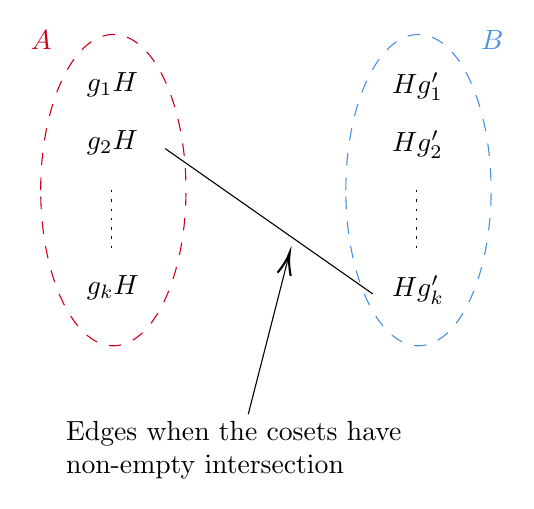
\begin{tikzpicture}[x=0.75pt,y=0.75pt,yscale=-1,xscale=1]
%uncomment if require: \path (0,273); %set diagram left start at 0, and has height of 273

%Straight Lines [id:da7801426772125396] 
\draw    (320,100) -- (420,170) ;
%Shape: Ellipse [id:dp934198625169717] 
\draw  [color={rgb, 255:red, 208; green, 2; blue, 27 }  ,draw opacity=1 ][dash pattern={on 4.5pt off 4.5pt}] (260,120) .. controls (260,78.58) and (275.67,45) .. (295,45) .. controls (314.33,45) and (330,78.58) .. (330,120) .. controls (330,161.42) and (314.33,195) .. (295,195) .. controls (275.67,195) and (260,161.42) .. (260,120) -- cycle ;
%Straight Lines [id:da28132709017632884] 
\draw  [dash pattern={on 0.84pt off 2.51pt}]  (294,120) -- (294,150) ;
%Shape: Ellipse [id:dp44431413928262453] 
\draw  [color={rgb, 255:red, 74; green, 144; blue, 226 }  ,draw opacity=1 ][dash pattern={on 4.5pt off 4.5pt}] (407,120) .. controls (407,78.58) and (422.67,45) .. (442,45) .. controls (461.33,45) and (477,78.58) .. (477,120) .. controls (477,161.42) and (461.33,195) .. (442,195) .. controls (422.67,195) and (407,161.42) .. (407,120) -- cycle ;
%Straight Lines [id:da30920045756292314] 
\draw  [dash pattern={on 0.84pt off 2.51pt}]  (441,120) -- (441,150) ;
%Straight Lines [id:da31804273242523373] 
\draw    (360,228) -- (379.5,151.94) ;
\draw [shift={(380,150)}, rotate = 464.38] [color={rgb, 255:red, 0; green, 0; blue, 0 }  ][line width=0.75]    (10.93,-3.29) .. controls (6.95,-1.4) and (3.31,-0.3) .. (0,0) .. controls (3.31,0.3) and (6.95,1.4) .. (10.93,3.29)   ;

% Text Node
\draw (254,42) node [anchor=north west][inner sep=0.75pt]    {$\textcolor[rgb]{0.82,0.01,0.11}{A}$};
% Text Node
\draw (281,62) node [anchor=north west][inner sep=0.75pt]    {$g_{1} H$};
% Text Node
\draw (281,90) node [anchor=north west][inner sep=0.75pt]    {$g_{2} H$};
% Text Node
\draw (281,160) node [anchor=north west][inner sep=0.75pt]    {$g_{k} H$};
% Text Node
\draw (471,42) node [anchor=north west][inner sep=0.75pt]  [color={rgb, 255:red, 74; green, 144; blue, 226 }  ,opacity=1 ]  {$B$};
% Text Node
\draw (428,62) node [anchor=north west][inner sep=0.75pt]    {$Hg_{1} '$};
% Text Node
\draw (428,90) node [anchor=north west][inner sep=0.75pt]    {$Hg_{2} '$};
% Text Node
\draw (428,160) node [anchor=north west][inner sep=0.75pt]    {$Hg_{k} '$};
% Text Node
\draw (271,230) node [anchor=north west][inner sep=0.75pt]   [align=left] {Edges when the cosets have \\non-empty intersection};


\end{tikzpicture}

\end{center}

If we had a perfect matching in this graph, then we could pick an element $h_i$ in the (non-empty) intersection of the matched left and right cosets, and then $h_1, \dots, h_k$ would be a set of coset representatives for all of the $k$ left and right cosets.

So we want to show that Hall's theorem is satisfied.
Given $I \subseteq \{1, \dots, k\}$, we want to show that the number of right cosets intersecting $\bigcup_{i \in I} g_i H$ is at least $|I|$.

Observe that $\left|\bigcup_{i \in I} g_i H\right| = |H| |I|$. Since the right cosets partition $G$, and each coset has size $|H|$, so the number of right cosets intersecting $\bigcup g_i H$ is at least $|I|$. Thus $|N(\{g_iH \mid i \in I\})| \geq |I|$, and thus Hall's theorem is satisfied, and we have a perfect matching in the graph.

\end{example}

\section{Connectivity}

We have already defined what it means for a graph to be connected, but consider the following connected graphs:

\begin{center}
	

\tikzset{every picture/.style={line width=0.75pt}} %set default line width to 0.75pt        

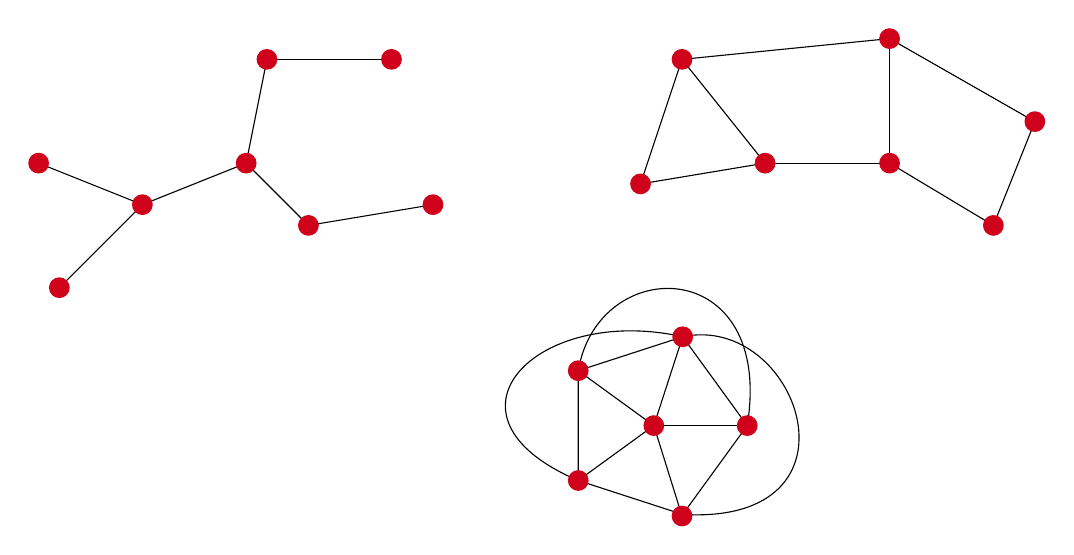
\begin{tikzpicture}[x=0.75pt,y=0.75pt,yscale=-1,xscale=1]
%uncomment if require: \path (0,293); %set diagram left start at 0, and has height of 293

%Curve Lines [id:da9294425428722793] 
\draw    (365.31,148.65) .. controls (421,136.8) and (457,239.6) .. (365.31,234.25) ;
%Curve Lines [id:da009421574300728985] 
\draw    (365.31,148.65) .. controls (295,132.8) and (241.8,186.8) .. (315,217.9) ;
%Curve Lines [id:da321087271165589] 
\draw    (315,165) .. controls (324.6,108) and (409.8,108.8) .. (396.41,191.45) ;
%Straight Lines [id:da18845335765002535] 
\draw    (351.41,191.45) -- (365.31,148.65) ;
%Straight Lines [id:da10868612639561437] 
\draw    (351.41,191.45) -- (396.41,191.45) ;
%Straight Lines [id:da5580509198085325] 
\draw    (351.41,191.45) -- (365,235) ;
%Straight Lines [id:da8517838287959706] 
\draw    (351.41,191.45) -- (315,217.9) ;
%Straight Lines [id:da817410490858483] 
\draw    (351.41,191.45) -- (315,165) ;
%Shape: Regular Polygon [id:dp18303747835997042] 
\draw   (396.41,191.45) -- (365.31,234.25) -- (315,217.9) -- (315,165) -- (365.31,148.65) -- cycle ;
%Straight Lines [id:da9467940880591912] 
\draw    (345,75) -- (405,65) ;
%Straight Lines [id:da07723253353686355] 
\draw    (365,15) -- (345,75) ;
%Straight Lines [id:da1549032891608607] 
\draw    (365,15) -- (405,65) ;
%Straight Lines [id:da7379993336466301] 
\draw    (405,65) -- (465,65) ;
%Straight Lines [id:da40906254738211056] 
\draw    (365,15) -- (465,5) ;
%Straight Lines [id:da770430691290185] 
\draw    (465,65) -- (465,5) ;
%Straight Lines [id:da6959373555522655] 
\draw    (515,95) -- (535,45) ;
%Straight Lines [id:da526742653904393] 
\draw    (465,65) -- (515,95) ;
%Straight Lines [id:da714176571195451] 
\draw    (465,5) -- (535,45) ;
%Straight Lines [id:da976390566478364] 
\draw    (55,65) -- (105,85) ;
%Straight Lines [id:da5578171554884205] 
\draw    (105,85) -- (155,65) ;
%Straight Lines [id:da7245091509249735] 
\draw    (105,85) -- (65,125) ;
%Straight Lines [id:da5704844096834922] 
\draw    (155,65) -- (165,15) ;
%Straight Lines [id:da9151309802279564] 
\draw    (165,15) -- (225,15) ;
%Straight Lines [id:da05754232518408475] 
\draw    (185,95) -- (245,85) ;
%Straight Lines [id:da8044154996629752] 
\draw    (155,65) -- (185,95) ;
%Shape: Circle [id:dp5691956835773179] 
\draw  [draw opacity=0][fill={rgb, 255:red, 208; green, 2; blue, 27 }  ,fill opacity=1 ] (50,65) .. controls (50,62.24) and (52.24,60) .. (55,60) .. controls (57.76,60) and (60,62.24) .. (60,65) .. controls (60,67.76) and (57.76,70) .. (55,70) .. controls (52.24,70) and (50,67.76) .. (50,65) -- cycle ;
%Shape: Circle [id:dp07989317854587785] 
\draw  [draw opacity=0][fill={rgb, 255:red, 208; green, 2; blue, 27 }  ,fill opacity=1 ] (60,125) .. controls (60,122.24) and (62.24,120) .. (65,120) .. controls (67.76,120) and (70,122.24) .. (70,125) .. controls (70,127.76) and (67.76,130) .. (65,130) .. controls (62.24,130) and (60,127.76) .. (60,125) -- cycle ;
%Shape: Circle [id:dp03198003583418951] 
\draw  [draw opacity=0][fill={rgb, 255:red, 208; green, 2; blue, 27 }  ,fill opacity=1 ] (100,85) .. controls (100,82.24) and (102.24,80) .. (105,80) .. controls (107.76,80) and (110,82.24) .. (110,85) .. controls (110,87.76) and (107.76,90) .. (105,90) .. controls (102.24,90) and (100,87.76) .. (100,85) -- cycle ;
%Shape: Circle [id:dp5745271354861535] 
\draw  [draw opacity=0][fill={rgb, 255:red, 208; green, 2; blue, 27 }  ,fill opacity=1 ] (160,15) .. controls (160,12.24) and (162.24,10) .. (165,10) .. controls (167.76,10) and (170,12.24) .. (170,15) .. controls (170,17.76) and (167.76,20) .. (165,20) .. controls (162.24,20) and (160,17.76) .. (160,15) -- cycle ;
%Shape: Circle [id:dp6345238812275618] 
\draw  [draw opacity=0][fill={rgb, 255:red, 208; green, 2; blue, 27 }  ,fill opacity=1 ] (180,95) .. controls (180,92.24) and (182.24,90) .. (185,90) .. controls (187.76,90) and (190,92.24) .. (190,95) .. controls (190,97.76) and (187.76,100) .. (185,100) .. controls (182.24,100) and (180,97.76) .. (180,95) -- cycle ;
%Shape: Circle [id:dp6607478220132026] 
\draw  [draw opacity=0][fill={rgb, 255:red, 208; green, 2; blue, 27 }  ,fill opacity=1 ] (220,15) .. controls (220,12.24) and (222.24,10) .. (225,10) .. controls (227.76,10) and (230,12.24) .. (230,15) .. controls (230,17.76) and (227.76,20) .. (225,20) .. controls (222.24,20) and (220,17.76) .. (220,15) -- cycle ;
%Shape: Circle [id:dp47922151410928704] 
\draw  [draw opacity=0][fill={rgb, 255:red, 208; green, 2; blue, 27 }  ,fill opacity=1 ] (240,85) .. controls (240,82.24) and (242.24,80) .. (245,80) .. controls (247.76,80) and (250,82.24) .. (250,85) .. controls (250,87.76) and (247.76,90) .. (245,90) .. controls (242.24,90) and (240,87.76) .. (240,85) -- cycle ;
%Shape: Circle [id:dp3302812426144347] 
\draw  [draw opacity=0][fill={rgb, 255:red, 208; green, 2; blue, 27 }  ,fill opacity=1 ] (150,65) .. controls (150,62.24) and (152.24,60) .. (155,60) .. controls (157.76,60) and (160,62.24) .. (160,65) .. controls (160,67.76) and (157.76,70) .. (155,70) .. controls (152.24,70) and (150,67.76) .. (150,65) -- cycle ;
%Shape: Circle [id:dp4052171710717183] 
\draw  [draw opacity=0][fill={rgb, 255:red, 208; green, 2; blue, 27 }  ,fill opacity=1 ] (360,15) .. controls (360,12.24) and (362.24,10) .. (365,10) .. controls (367.76,10) and (370,12.24) .. (370,15) .. controls (370,17.76) and (367.76,20) .. (365,20) .. controls (362.24,20) and (360,17.76) .. (360,15) -- cycle ;
%Shape: Circle [id:dp10844632028565848] 
\draw  [draw opacity=0][fill={rgb, 255:red, 208; green, 2; blue, 27 }  ,fill opacity=1 ] (340,75) .. controls (340,72.24) and (342.24,70) .. (345,70) .. controls (347.76,70) and (350,72.24) .. (350,75) .. controls (350,77.76) and (347.76,80) .. (345,80) .. controls (342.24,80) and (340,77.76) .. (340,75) -- cycle ;
%Shape: Circle [id:dp8345428281532884] 
\draw  [draw opacity=0][fill={rgb, 255:red, 208; green, 2; blue, 27 }  ,fill opacity=1 ] (400,65) .. controls (400,62.24) and (402.24,60) .. (405,60) .. controls (407.76,60) and (410,62.24) .. (410,65) .. controls (410,67.76) and (407.76,70) .. (405,70) .. controls (402.24,70) and (400,67.76) .. (400,65) -- cycle ;
%Shape: Circle [id:dp7978283937865467] 
\draw  [draw opacity=0][fill={rgb, 255:red, 208; green, 2; blue, 27 }  ,fill opacity=1 ] (460,5) .. controls (460,2.24) and (462.24,0) .. (465,0) .. controls (467.76,0) and (470,2.24) .. (470,5) .. controls (470,7.76) and (467.76,10) .. (465,10) .. controls (462.24,10) and (460,7.76) .. (460,5) -- cycle ;
%Shape: Circle [id:dp12955913420965248] 
\draw  [draw opacity=0][fill={rgb, 255:red, 208; green, 2; blue, 27 }  ,fill opacity=1 ] (460,65) .. controls (460,62.24) and (462.24,60) .. (465,60) .. controls (467.76,60) and (470,62.24) .. (470,65) .. controls (470,67.76) and (467.76,70) .. (465,70) .. controls (462.24,70) and (460,67.76) .. (460,65) -- cycle ;
%Shape: Circle [id:dp9262390680975451] 
\draw  [draw opacity=0][fill={rgb, 255:red, 208; green, 2; blue, 27 }  ,fill opacity=1 ] (530,45) .. controls (530,42.24) and (532.24,40) .. (535,40) .. controls (537.76,40) and (540,42.24) .. (540,45) .. controls (540,47.76) and (537.76,50) .. (535,50) .. controls (532.24,50) and (530,47.76) .. (530,45) -- cycle ;
%Shape: Circle [id:dp928311621735886] 
\draw  [draw opacity=0][fill={rgb, 255:red, 208; green, 2; blue, 27 }  ,fill opacity=1 ] (510,95) .. controls (510,92.24) and (512.24,90) .. (515,90) .. controls (517.76,90) and (520,92.24) .. (520,95) .. controls (520,97.76) and (517.76,100) .. (515,100) .. controls (512.24,100) and (510,97.76) .. (510,95) -- cycle ;
%Shape: Circle [id:dp755801932679404] 
\draw  [draw opacity=0][fill={rgb, 255:red, 208; green, 2; blue, 27 }  ,fill opacity=1 ] (310,165) .. controls (310,162.24) and (312.24,160) .. (315,160) .. controls (317.76,160) and (320,162.24) .. (320,165) .. controls (320,167.76) and (317.76,170) .. (315,170) .. controls (312.24,170) and (310,167.76) .. (310,165) -- cycle ;
%Shape: Circle [id:dp1954939443227529] 
\draw  [draw opacity=0][fill={rgb, 255:red, 208; green, 2; blue, 27 }  ,fill opacity=1 ] (360.31,148.65) .. controls (360.31,145.89) and (362.55,143.65) .. (365.31,143.65) .. controls (368.07,143.65) and (370.31,145.89) .. (370.31,148.65) .. controls (370.31,151.41) and (368.07,153.65) .. (365.31,153.65) .. controls (362.55,153.65) and (360.31,151.41) .. (360.31,148.65) -- cycle ;
%Shape: Circle [id:dp5604701768083181] 
\draw  [draw opacity=0][fill={rgb, 255:red, 208; green, 2; blue, 27 }  ,fill opacity=1 ] (310,217.9) .. controls (310,215.14) and (312.24,212.9) .. (315,212.9) .. controls (317.76,212.9) and (320,215.14) .. (320,217.9) .. controls (320,220.66) and (317.76,222.9) .. (315,222.9) .. controls (312.24,222.9) and (310,220.66) .. (310,217.9) -- cycle ;
%Shape: Circle [id:dp19589468689495915] 
\draw  [draw opacity=0][fill={rgb, 255:red, 208; green, 2; blue, 27 }  ,fill opacity=1 ] (360,235) .. controls (360,232.24) and (362.24,230) .. (365,230) .. controls (367.76,230) and (370,232.24) .. (370,235) .. controls (370,237.76) and (367.76,240) .. (365,240) .. controls (362.24,240) and (360,237.76) .. (360,235) -- cycle ;
%Shape: Circle [id:dp8976613146147098] 
\draw  [draw opacity=0][fill={rgb, 255:red, 208; green, 2; blue, 27 }  ,fill opacity=1 ] (391.41,191.45) .. controls (391.41,188.69) and (393.64,186.45) .. (396.41,186.45) .. controls (399.17,186.45) and (401.41,188.69) .. (401.41,191.45) .. controls (401.41,194.21) and (399.17,196.45) .. (396.41,196.45) .. controls (393.64,196.45) and (391.41,194.21) .. (391.41,191.45) -- cycle ;
%Shape: Circle [id:dp46320584092219275] 
\draw  [draw opacity=0][fill={rgb, 255:red, 208; green, 2; blue, 27 }  ,fill opacity=1 ] (346.41,191.45) .. controls (346.41,188.69) and (348.64,186.45) .. (351.41,186.45) .. controls (354.17,186.45) and (356.41,188.69) .. (356.41,191.45) .. controls (356.41,194.21) and (354.17,196.45) .. (351.41,196.45) .. controls (348.64,196.45) and (346.41,194.21) .. (346.41,191.45) -- cycle ;




\end{tikzpicture}

\end{center}

Clearly these are connected, but they are all `connected to different extents'. For example, in the first graph, removing any vertex disconnects the graph. In the second graph, any vertex could be removed and the graph would stay connected. We can also see that in the first graph, there's only one path from one vertex to another, whereas in the third graph there is many. This also seems to correlate with `how connected' a graph is.

\subsection{Measuring Connectivity}

So looking at the graphs above, we two natural notions for `how connected a graph is' can be informally described as
\begin{enumerate}
	\item A `deletion notion' of connectivity, where we consider how connected the graph is after some vertices are removed.
	\item A `paths notion' of connectivity, where we consider how many independent paths there is between vertices.
\end{enumerate}

One of the main goals of this section will be turning this vague notion into a concrete concept, and proving an interesting result about how the two notions relate to each other.

\begin{notation}[Removing Vertex Sets]
	In this section (and for the rest of this article), if $G = (V, E)$ is a graph and $S \subseteq V$, we define $G - S = G - x_1 - x_2 - \cdots - x_l$ where $S = \{x_1, \dots, x_l\}$.
\end{notation}

We will begin with a definition.

\begin{definition}[Cut Vertex]
Let $G = (V, E)$ be a connected graph. We say that $v \in V$ is a \vocab{cut vertex} if $G - v$ is disconnected.	
\end{definition}

\begin{center}
	

\tikzset{every picture/.style={line width=0.75pt}} %set default line width to 0.75pt        

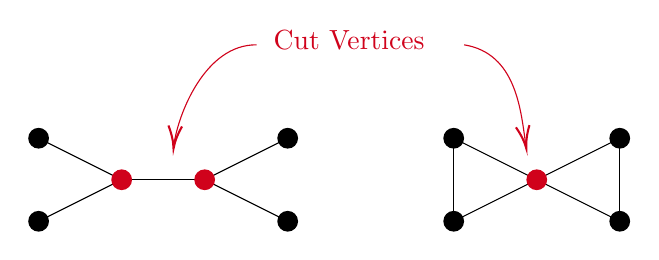
\begin{tikzpicture}[x=0.75pt,y=0.75pt,yscale=-1,xscale=1]
%uncomment if require: \path (0,293); %set diagram left start at 0, and has height of 293

%Shape: Circle [id:dp12745017121991498] 
\draw  [draw opacity=0][fill={rgb, 255:red, 0; green, 0; blue, 0 }  ,fill opacity=1 ] (80,175) .. controls (80,172.24) and (82.24,170) .. (85,170) .. controls (87.76,170) and (90,172.24) .. (90,175) .. controls (90,177.76) and (87.76,180) .. (85,180) .. controls (82.24,180) and (80,177.76) .. (80,175) -- cycle ;
%Shape: Circle [id:dp9076984940922347] 
\draw  [draw opacity=0][fill={rgb, 255:red, 0; green, 0; blue, 0 }  ,fill opacity=1 ] (80,215) .. controls (80,212.24) and (82.24,210) .. (85,210) .. controls (87.76,210) and (90,212.24) .. (90,215) .. controls (90,217.76) and (87.76,220) .. (85,220) .. controls (82.24,220) and (80,217.76) .. (80,215) -- cycle ;
%Shape: Circle [id:dp04965646309582172] 
\draw  [draw opacity=0][fill={rgb, 255:red, 0; green, 0; blue, 0 }  ,fill opacity=1 ] (200,175) .. controls (200,172.24) and (202.24,170) .. (205,170) .. controls (207.76,170) and (210,172.24) .. (210,175) .. controls (210,177.76) and (207.76,180) .. (205,180) .. controls (202.24,180) and (200,177.76) .. (200,175) -- cycle ;
%Shape: Circle [id:dp8898793626929573] 
\draw  [draw opacity=0][fill={rgb, 255:red, 0; green, 0; blue, 0 }  ,fill opacity=1 ] (200,215) .. controls (200,212.24) and (202.24,210) .. (205,210) .. controls (207.76,210) and (210,212.24) .. (210,215) .. controls (210,217.76) and (207.76,220) .. (205,220) .. controls (202.24,220) and (200,217.76) .. (200,215) -- cycle ;
%Straight Lines [id:da5382527615587057] 
\draw [fill={rgb, 255:red, 0; green, 0; blue, 0 }  ,fill opacity=1 ]   (85,175) -- (125,195) ;
%Straight Lines [id:da7659680646322984] 
\draw [fill={rgb, 255:red, 0; green, 0; blue, 0 }  ,fill opacity=1 ]   (125,195) -- (165,195) ;
%Straight Lines [id:da2312977972871566] 
\draw [fill={rgb, 255:red, 0; green, 0; blue, 0 }  ,fill opacity=1 ]   (165,195) -- (205,175) ;
%Straight Lines [id:da39871333523269936] 
\draw [fill={rgb, 255:red, 0; green, 0; blue, 0 }  ,fill opacity=1 ]   (205,215) -- (165,195) ;
%Straight Lines [id:da06003935166791907] 
\draw [fill={rgb, 255:red, 0; green, 0; blue, 0 }  ,fill opacity=1 ]   (125,195) -- (85,215) ;
%Shape: Circle [id:dp6056530051711337] 
\draw  [draw opacity=0][fill={rgb, 255:red, 208; green, 2; blue, 27 }  ,fill opacity=1 ] (120,195) .. controls (120,192.24) and (122.24,190) .. (125,190) .. controls (127.76,190) and (130,192.24) .. (130,195) .. controls (130,197.76) and (127.76,200) .. (125,200) .. controls (122.24,200) and (120,197.76) .. (120,195) -- cycle ;
%Shape: Circle [id:dp35313026814601167] 
\draw  [draw opacity=0][fill={rgb, 255:red, 208; green, 2; blue, 27 }  ,fill opacity=1 ] (160,195) .. controls (160,192.24) and (162.24,190) .. (165,190) .. controls (167.76,190) and (170,192.24) .. (170,195) .. controls (170,197.76) and (167.76,200) .. (165,200) .. controls (162.24,200) and (160,197.76) .. (160,195) -- cycle ;
%Shape: Circle [id:dp647823679665335] 
\draw  [draw opacity=0][fill={rgb, 255:red, 0; green, 0; blue, 0 }  ,fill opacity=1 ] (280,175) .. controls (280,172.24) and (282.24,170) .. (285,170) .. controls (287.76,170) and (290,172.24) .. (290,175) .. controls (290,177.76) and (287.76,180) .. (285,180) .. controls (282.24,180) and (280,177.76) .. (280,175) -- cycle ;
%Shape: Circle [id:dp7146264689498645] 
\draw  [draw opacity=0][fill={rgb, 255:red, 0; green, 0; blue, 0 }  ,fill opacity=1 ] (280,215) .. controls (280,212.24) and (282.24,210) .. (285,210) .. controls (287.76,210) and (290,212.24) .. (290,215) .. controls (290,217.76) and (287.76,220) .. (285,220) .. controls (282.24,220) and (280,217.76) .. (280,215) -- cycle ;
%Shape: Circle [id:dp1527194288089806] 
\draw  [draw opacity=0][fill={rgb, 255:red, 0; green, 0; blue, 0 }  ,fill opacity=1 ] (360,175) .. controls (360,172.24) and (362.24,170) .. (365,170) .. controls (367.76,170) and (370,172.24) .. (370,175) .. controls (370,177.76) and (367.76,180) .. (365,180) .. controls (362.24,180) and (360,177.76) .. (360,175) -- cycle ;
%Shape: Circle [id:dp1903220915203041] 
\draw  [draw opacity=0][fill={rgb, 255:red, 0; green, 0; blue, 0 }  ,fill opacity=1 ] (360,215) .. controls (360,212.24) and (362.24,210) .. (365,210) .. controls (367.76,210) and (370,212.24) .. (370,215) .. controls (370,217.76) and (367.76,220) .. (365,220) .. controls (362.24,220) and (360,217.76) .. (360,215) -- cycle ;
%Straight Lines [id:da4565723920327317] 
\draw [fill={rgb, 255:red, 0; green, 0; blue, 0 }  ,fill opacity=1 ]   (285,175) -- (325,195) ;
%Straight Lines [id:da45703482917070415] 
\draw [fill={rgb, 255:red, 0; green, 0; blue, 0 }  ,fill opacity=1 ]   (325,195) -- (365,175) ;
%Straight Lines [id:da33078536414228965] 
\draw [fill={rgb, 255:red, 0; green, 0; blue, 0 }  ,fill opacity=1 ]   (365,215) -- (325,195) ;
%Straight Lines [id:da46639833976845313] 
\draw [fill={rgb, 255:red, 0; green, 0; blue, 0 }  ,fill opacity=1 ]   (325,195) -- (285,215) ;
%Shape: Circle [id:dp21667152621491192] 
\draw  [draw opacity=0][fill={rgb, 255:red, 208; green, 2; blue, 27 }  ,fill opacity=1 ] (320,195) .. controls (320,192.24) and (322.24,190) .. (325,190) .. controls (327.76,190) and (330,192.24) .. (330,195) .. controls (330,197.76) and (327.76,200) .. (325,200) .. controls (322.24,200) and (320,197.76) .. (320,195) -- cycle ;
%Straight Lines [id:da2363755483848876] 
\draw [fill={rgb, 255:red, 0; green, 0; blue, 0 }  ,fill opacity=1 ]   (285,215) -- (285,175) ;
%Straight Lines [id:da4318452178498824] 
\draw [fill={rgb, 255:red, 0; green, 0; blue, 0 }  ,fill opacity=1 ]   (365,215) -- (365,175) ;
%Curve Lines [id:da22420478286814505] 
\draw [color={rgb, 255:red, 208; green, 2; blue, 27 }  ,draw opacity=1 ]   (190,130) .. controls (165.17,129.76) and (152.2,163.5) .. (150.21,178.07) ;
\draw [shift={(150,180)}, rotate = 274.32] [color={rgb, 255:red, 208; green, 2; blue, 27 }  ,draw opacity=1 ][line width=0.75]    (10.93,-3.29) .. controls (6.95,-1.4) and (3.31,-0.3) .. (0,0) .. controls (3.31,0.3) and (6.95,1.4) .. (10.93,3.29)   ;
%Curve Lines [id:da3533900283623045] 
\draw [color={rgb, 255:red, 208; green, 2; blue, 27 }  ,draw opacity=1 ]   (290,130) .. controls (315.44,134.08) and (317.38,162.35) .. (319.71,178.1) ;
\draw [shift={(320,180)}, rotate = 260.69] [color={rgb, 255:red, 208; green, 2; blue, 27 }  ,draw opacity=1 ][line width=0.75]    (10.93,-3.29) .. controls (6.95,-1.4) and (3.31,-0.3) .. (0,0) .. controls (3.31,0.3) and (6.95,1.4) .. (10.93,3.29)   ;

% Text Node
\draw (197,122) node [anchor=north west][inner sep=0.75pt]  [color={rgb, 255:red, 208; green, 2; blue, 27 }  ,opacity=1 ] [align=left] {Cut Vertices};


\end{tikzpicture}

\end{center}

\begin{definition}[Seperator]
	If $G = (G, V)$ is a connected graph, we say that a subset $S \subseteq V$ is a \vocab{separator} (or separating set) if $G - S$ is disconnected.
\end{definition}

With these concepts defined, we can define our `deletion' notion of connectivity.

\begin{definition}[Connectivity]
	Let $G = (V, E)$ be a graph. The \vocab{connectivity} of $G$, denoted $\kappa(G)$, is the size of the smallest set $S \subseteq V$ such that $G - S$ is disconnected, or just a single vertex\footnote{This is needed for the case of a complete graph.}.
\end{definition}
\begin{example}[Connectivity of $C_n$]
	Consider the graph $C_n$ for $n \geq 3$.
	\begin{center}
		

\tikzset{every picture/.style={line width=0.75pt}} %set default line width to 0.75pt        

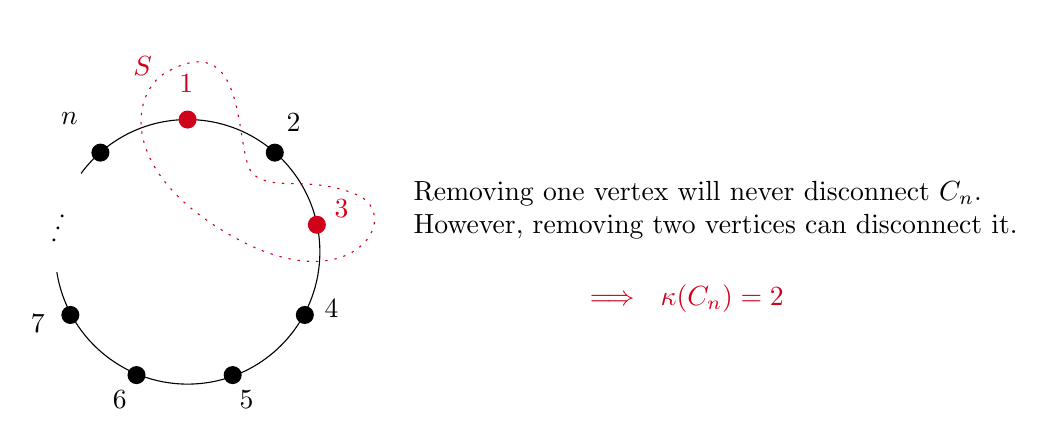
\begin{tikzpicture}[x=0.75pt,y=0.75pt,yscale=-1,xscale=1]
%uncomment if require: \path (0,244); %set diagram left start at 0, and has height of 244

%Shape: Arc [id:dp4708029626642417] 
\draw  [draw opacity=0] (147.09,79.71) .. controls (158.69,63.97) and (177.36,53.75) .. (198.42,53.75) .. controls (233.62,53.75) and (262.15,82.28) .. (262.15,117.48) .. controls (262.15,152.68) and (233.62,181.21) .. (198.42,181.21) .. controls (166.53,181.21) and (140.11,157.77) .. (135.43,127.19) -- (198.42,117.48) -- cycle ; \draw   (147.09,79.71) .. controls (158.69,63.97) and (177.36,53.75) .. (198.42,53.75) .. controls (233.62,53.75) and (262.15,82.28) .. (262.15,117.48) .. controls (262.15,152.68) and (233.62,181.21) .. (198.42,181.21) .. controls (166.53,181.21) and (140.11,157.77) .. (135.43,127.19) ;
%Shape: Ellipse [id:dp663608297444586] 
\draw  [draw opacity=0][fill={rgb, 255:red, 208; green, 2; blue, 27 }  ,fill opacity=1 ] (194.08,53.75) .. controls (194.08,51.35) and (196.02,49.41) .. (198.42,49.41) .. controls (200.82,49.41) and (202.77,51.35) .. (202.77,53.75) .. controls (202.77,56.15) and (200.82,58.1) .. (198.42,58.1) .. controls (196.02,58.1) and (194.08,56.15) .. (194.08,53.75) -- cycle ;
%Shape: Ellipse [id:dp6954182191954329] 
\draw  [draw opacity=0][fill={rgb, 255:red, 0; green, 0; blue, 0 }  ,fill opacity=1 ] (236.08,69.68) .. controls (236.08,67.28) and (238.03,65.34) .. (240.43,65.34) .. controls (242.83,65.34) and (244.77,67.28) .. (244.77,69.68) .. controls (244.77,72.08) and (242.83,74.03) .. (240.43,74.03) .. controls (238.03,74.03) and (236.08,72.08) .. (236.08,69.68) -- cycle ;
%Shape: Circle [id:dp9749161979355754] 
\draw  [draw opacity=0][fill={rgb, 255:red, 208; green, 2; blue, 27 }  ,fill opacity=1 ] (256.36,104.44) .. controls (256.36,102.04) and (258.3,100.1) .. (260.7,100.1) .. controls (263.1,100.1) and (265.05,102.04) .. (265.05,104.44) .. controls (265.05,106.84) and (263.1,108.79) .. (260.7,108.79) .. controls (258.3,108.79) and (256.36,106.84) .. (256.36,104.44) -- cycle ;
%Shape: Ellipse [id:dp42403131489300416] 
\draw  [draw opacity=0][fill={rgb, 255:red, 0; green, 0; blue, 0 }  ,fill opacity=1 ] (250.56,147.89) .. controls (250.56,145.5) and (252.51,143.55) .. (254.91,143.55) .. controls (257.31,143.55) and (259.25,145.5) .. (259.25,147.89) .. controls (259.25,150.29) and (257.31,152.24) .. (254.91,152.24) .. controls (252.51,152.24) and (250.56,150.29) .. (250.56,147.89) -- cycle ;
%Shape: Circle [id:dp735948108869646] 
\draw  [draw opacity=0][fill={rgb, 255:red, 0; green, 0; blue, 0 }  ,fill opacity=1 ] (215.8,176.86) .. controls (215.8,174.46) and (217.75,172.52) .. (220.15,172.52) .. controls (222.55,172.52) and (224.49,174.46) .. (224.49,176.86) .. controls (224.49,179.26) and (222.55,181.21) .. (220.15,181.21) .. controls (217.75,181.21) and (215.8,179.26) .. (215.8,176.86) -- cycle ;
%Shape: Circle [id:dp361614150375666] 
\draw  [draw opacity=0][fill={rgb, 255:red, 0; green, 0; blue, 0 }  ,fill opacity=1 ] (169.46,176.86) .. controls (169.46,174.46) and (171.4,172.52) .. (173.8,172.52) .. controls (176.2,172.52) and (178.15,174.46) .. (178.15,176.86) .. controls (178.15,179.26) and (176.2,181.21) .. (173.8,181.21) .. controls (171.4,181.21) and (169.46,179.26) .. (169.46,176.86) -- cycle ;
%Shape: Ellipse [id:dp799299292223014] 
\draw  [draw opacity=0][fill={rgb, 255:red, 0; green, 0; blue, 0 }  ,fill opacity=1 ] (137.59,147.89) .. controls (137.59,145.5) and (139.54,143.55) .. (141.94,143.55) .. controls (144.34,143.55) and (146.28,145.5) .. (146.28,147.89) .. controls (146.28,150.29) and (144.34,152.24) .. (141.94,152.24) .. controls (139.54,152.24) and (137.59,150.29) .. (137.59,147.89) -- cycle ;
%Shape: Rectangle [id:dp5189451174903476] 
\draw  [draw opacity=0][fill={rgb, 255:red, 255; green, 255; blue, 255 }  ,fill opacity=0 ] (123.11,76.93) -- (163.66,76.93) -- (163.66,123.27) -- (123.11,123.27) -- cycle ;
%Shape: Ellipse [id:dp2783474184800838] 
\draw  [draw opacity=0][fill={rgb, 255:red, 0; green, 0; blue, 0 }  ,fill opacity=1 ] (152.08,69.68) .. controls (152.08,67.28) and (154.02,65.34) .. (156.42,65.34) .. controls (158.82,65.34) and (160.77,67.28) .. (160.77,69.68) .. controls (160.77,72.08) and (158.82,74.03) .. (156.42,74.03) .. controls (154.02,74.03) and (152.08,72.08) .. (152.08,69.68) -- cycle ;
%Curve Lines [id:da09228568553946859] 
\draw [color={rgb, 255:red, 208; green, 2; blue, 27 }  ,draw opacity=1 ] [dash pattern={on 0.84pt off 2.51pt}]  (190,30) .. controls (229,9.75) and (220.5,71.25) .. (230,80) .. controls (239.5,88.75) and (257,80.25) .. (280,90) .. controls (303,99.75) and (278,142.75) .. (220,110) .. controls (162,77.25) and (172,37.75) .. (190,30) -- cycle ;

% Text Node
\draw (131.16,114.02) node [anchor=north west][inner sep=0.75pt]  [rotate=-289.59]  {$\dotsc $};
% Text Node
\draw (193.17,31) node [anchor=north west][inner sep=0.75pt]  [color={rgb, 255:red, 208; green, 2; blue, 27 }  ,opacity=1 ]  {$1$};
% Text Node
\draw (244.83,49.55) node [anchor=north west][inner sep=0.75pt]    {$2$};
% Text Node
\draw (268,91.1) node [anchor=north west][inner sep=0.75pt]  [color={rgb, 255:red, 208; green, 2; blue, 27 }  ,opacity=1 ]  {$3$};
% Text Node
\draw (263.21,139.45) node [anchor=north west][inner sep=0.75pt]    {$4$};
% Text Node
\draw (222.17,183) node [anchor=north west][inner sep=0.75pt]    {$5$};
% Text Node
\draw (161.2,183) node [anchor=north west][inner sep=0.75pt]    {$6$};
% Text Node
\draw (121.64,146.45) node [anchor=north west][inner sep=0.75pt]    {$7$};
% Text Node
\draw (136.17,49) node [anchor=north west][inner sep=0.75pt]    {$n$};
% Text Node
\draw (306,82) node [anchor=north west][inner sep=0.75pt]   [align=left] {Removing one vertex will never disconnect $\displaystyle C_{n}$.\\However, removing two vertices can disconnect it.};
% Text Node
\draw (391,132) node [anchor=north west][inner sep=0.75pt]  [color={rgb, 255:red, 208; green, 2; blue, 27 }  ,opacity=1 ]  {$\Longrightarrow \ \ \kappa ( C_{n}) =2$};
% Text Node
\draw (171,22) node [anchor=north west][inner sep=0.75pt]  [color={rgb, 255:red, 208; green, 2; blue, 27 }  ,opacity=1 ]  {$S$};


\end{tikzpicture}
	\end{center}
	
\end{example}

\begin{example}[Connectivity of the Petersen Graph]
	We define the \vocab{Petersen graph} with 10 vertices and 15 edges as shown below.
	\begin{center}
		

\tikzset{every picture/.style={line width=0.75pt}} %set default line width to 0.75pt        

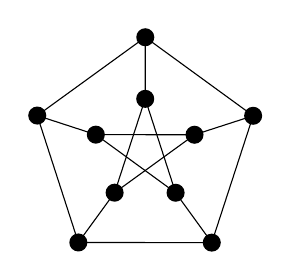
\begin{tikzpicture}[x=0.75pt,y=0.75pt,yscale=-1,xscale=1]
%uncomment if require: \path (0,244); %set diagram left start at 0, and has height of 244

%Shape: Regular Polygon [id:dp05983163114582302] 
\draw  [color={rgb, 255:red, 0; green, 0; blue, 0 }  ,draw opacity=1 ] (333.51,89.24) -- (313.58,150.35) -- (249.3,150.29) -- (229.5,89.13) -- (281.54,51.4) -- cycle ;
%Shape: Regular Polygon [id:dp2169015140813345] 
\draw  [draw opacity=0] (305.27,98.38) -- (296.16,126.32) -- (266.77,126.29) -- (257.72,98.33) -- (281.51,81.08) -- cycle ;
%Shape: Ellipse [id:dp2284299806952339] 
\draw  [draw opacity=0][fill={rgb, 255:red, 0; green, 0; blue, 0 }  ,fill opacity=1 ] (277.17,81.08) .. controls (277.17,78.68) and (279.11,76.74) .. (281.51,76.74) .. controls (283.91,76.74) and (285.86,78.68) .. (285.86,81.08) .. controls (285.86,83.48) and (283.91,85.43) .. (281.51,85.43) .. controls (279.11,85.43) and (277.17,83.48) .. (277.17,81.08) -- cycle ;
%Shape: Ellipse [id:dp7834602075108992] 
\draw  [draw opacity=0][fill={rgb, 255:red, 0; green, 0; blue, 0 }  ,fill opacity=1 ] (253.37,98.33) .. controls (253.37,95.93) and (255.32,93.99) .. (257.72,93.99) .. controls (260.12,93.99) and (262.06,95.93) .. (262.06,98.33) .. controls (262.06,100.73) and (260.12,102.68) .. (257.72,102.68) .. controls (255.32,102.68) and (253.37,100.73) .. (253.37,98.33) -- cycle ;
%Shape: Ellipse [id:dp10631586731654152] 
\draw  [draw opacity=0][fill={rgb, 255:red, 0; green, 0; blue, 0 }  ,fill opacity=1 ] (262.42,126.29) .. controls (262.42,123.89) and (264.37,121.95) .. (266.77,121.95) .. controls (269.17,121.95) and (271.11,123.89) .. (271.11,126.29) .. controls (271.11,128.69) and (269.17,130.64) .. (266.77,130.64) .. controls (264.37,130.64) and (262.42,128.69) .. (262.42,126.29) -- cycle ;
%Shape: Ellipse [id:dp8855198554358988] 
\draw  [draw opacity=0][fill={rgb, 255:red, 0; green, 0; blue, 0 }  ,fill opacity=1 ] (291.81,126.32) .. controls (291.81,123.93) and (293.76,121.98) .. (296.16,121.98) .. controls (298.56,121.98) and (300.5,123.93) .. (300.5,126.32) .. controls (300.5,128.72) and (298.56,130.67) .. (296.16,130.67) .. controls (293.76,130.67) and (291.81,128.72) .. (291.81,126.32) -- cycle ;
%Shape: Ellipse [id:dp5274077183232346] 
\draw  [draw opacity=0][fill={rgb, 255:red, 0; green, 0; blue, 0 }  ,fill opacity=1 ] (300.92,98.38) .. controls (300.92,95.98) and (302.87,94.04) .. (305.27,94.04) .. controls (307.67,94.04) and (309.61,95.98) .. (309.61,98.38) .. controls (309.61,100.78) and (307.67,102.73) .. (305.27,102.73) .. controls (302.87,102.73) and (300.92,100.78) .. (300.92,98.38) -- cycle ;
%Straight Lines [id:da9145731591262345] 
\draw    (257.72,98.33) -- (305.27,98.38) ;
%Straight Lines [id:da286550976504756] 
\draw    (281.51,81.08) -- (296.16,126.32) ;
%Straight Lines [id:da3216010808629356] 
\draw    (305.27,98.38) -- (266.77,126.29) ;
%Straight Lines [id:da6884731409915993] 
\draw    (257.72,98.33) -- (296.16,126.32) ;
%Straight Lines [id:da5549242542450014] 
\draw    (281.51,81.08) -- (266.77,126.29) ;
%Shape: Ellipse [id:dp3903755840266917] 
\draw  [draw opacity=0][fill={rgb, 255:red, 0; green, 0; blue, 0 }  ,fill opacity=1 ] (225.15,89.13) .. controls (225.15,86.73) and (227.1,84.79) .. (229.5,84.79) .. controls (231.9,84.79) and (233.84,86.73) .. (233.84,89.13) .. controls (233.84,91.53) and (231.9,93.48) .. (229.5,93.48) .. controls (227.1,93.48) and (225.15,91.53) .. (225.15,89.13) -- cycle ;
%Shape: Ellipse [id:dp7538567399869548] 
\draw  [draw opacity=0][fill={rgb, 255:red, 0; green, 0; blue, 0 }  ,fill opacity=1 ] (277.2,51.4) .. controls (277.2,49) and (279.14,47.06) .. (281.54,47.06) .. controls (283.94,47.06) and (285.89,49) .. (285.89,51.4) .. controls (285.89,53.8) and (283.94,55.75) .. (281.54,55.75) .. controls (279.14,55.75) and (277.2,53.8) .. (277.2,51.4) -- cycle ;
%Shape: Ellipse [id:dp508221099123634] 
\draw  [draw opacity=0][fill={rgb, 255:red, 0; green, 0; blue, 0 }  ,fill opacity=1 ] (329.16,89.24) .. controls (329.16,86.84) and (331.11,84.9) .. (333.51,84.9) .. controls (335.91,84.9) and (337.85,86.84) .. (337.85,89.24) .. controls (337.85,91.64) and (335.91,93.59) .. (333.51,93.59) .. controls (331.11,93.59) and (329.16,91.64) .. (329.16,89.24) -- cycle ;
%Shape: Ellipse [id:dp5783697772918077] 
\draw  [draw opacity=0][fill={rgb, 255:red, 0; green, 0; blue, 0 }  ,fill opacity=1 ] (309.23,150.35) .. controls (309.23,147.95) and (311.18,146.01) .. (313.58,146.01) .. controls (315.98,146.01) and (317.92,147.95) .. (317.92,150.35) .. controls (317.92,152.75) and (315.98,154.7) .. (313.58,154.7) .. controls (311.18,154.7) and (309.23,152.75) .. (309.23,150.35) -- cycle ;
%Shape: Ellipse [id:dp6437731763387987] 
\draw  [draw opacity=0][fill={rgb, 255:red, 0; green, 0; blue, 0 }  ,fill opacity=1 ] (244.95,150.29) .. controls (244.95,147.89) and (246.9,145.94) .. (249.3,145.94) .. controls (251.7,145.94) and (253.64,147.89) .. (253.64,150.29) .. controls (253.64,152.69) and (251.7,154.63) .. (249.3,154.63) .. controls (246.9,154.63) and (244.95,152.69) .. (244.95,150.29) -- cycle ;
%Straight Lines [id:da6383337746934241] 
\draw    (229.5,89.13) -- (257.72,98.33) ;
%Straight Lines [id:da24335746175322703] 
\draw    (281.51,81.08) -- (281.54,51.4) ;
%Straight Lines [id:da8659383819038615] 
\draw    (333.51,89.24) -- (305.27,98.38) ;
%Straight Lines [id:da3992218809792242] 
\draw    (313.58,150.35) -- (296.16,126.32) ;
%Straight Lines [id:da4058518418803184] 
\draw    (249.3,150.29) -- (266.77,126.29) ;




\end{tikzpicture}

	\end{center}
We can see that the connectivity is at most $3$, since that is the degree of each vertex, and also removing two vertices won't disconnect the graph. Thus the connectivity of the Petersen graph is exactly 3.
\end{example}

\begin{definition}[$k$-Connected]
We say that a graph $G$ is \vocab{$k$-connected} if $\kappa(G) \geq k$. In particular, any set $S \leq V(G)$ with $|S| < k$	will have $G - S$ connected.
\end{definition}

We note this immediately implies that $G$ is 1-connected if and only if it's connected, and it is 2-connected if and only if it has no cut vertex.

We can note some basic properties of connnectivity.

\begin{lemma}[Increasing/Reducing Connectivity]
	If $G = (V, E)$ is a $k$-connected graph and $v \in V$ then $G - v$ is $(k - 1)$-connected\footnote{Note that it is also possible that $G - v$ is $(k + 1)$-connected, so connectivity can also increase by deleting a vertex.}. 
	Also, if we have some $e \in E$, then $G - E$ is $(k - 1)$-connected.
\end{lemma}
\begin{proof}[Proof Sketch]
Check definitions.
\end{proof}

\subsection{Preparing for Menger's Theorem}

We are going to prove Menger's theorem about connectivity measures, but we have to do some setting up beforehand.

\begin{definition}[$ab$-Seperator]
	If $G = (V, E)$ is a graph and $a, b \in V$ are distinct vertices, we say that $S$ is an \vocab{$ab$ seperator} if $a$ and $b$ lie in different components of $G - S$ (so $a, b \not \in S$).
\end{definition}
\begin{center}
	

\tikzset{every picture/.style={line width=0.75pt}} %set default line width to 0.75pt        

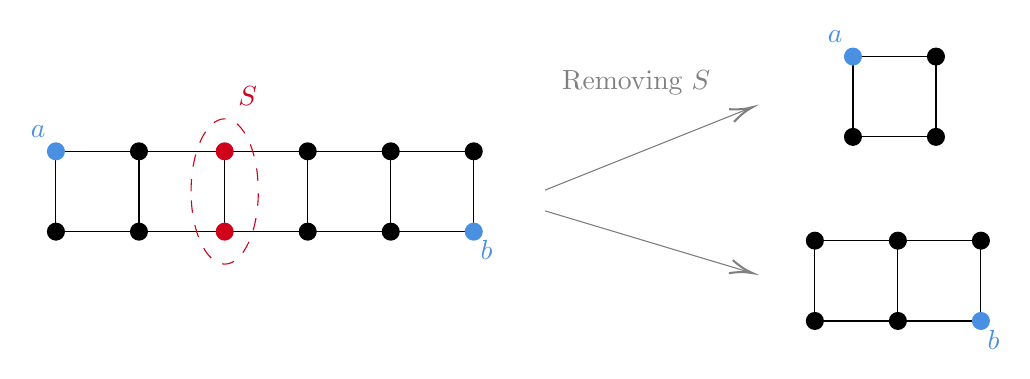
\begin{tikzpicture}[x=0.75pt,y=0.75pt,yscale=-1,xscale=1]
%uncomment if require: \path (0,244); %set diagram left start at 0, and has height of 244

%Shape: Ellipse [id:dp5456884071329711] 
\draw  [draw opacity=0][fill={rgb, 255:red, 0; green, 0; blue, 0 }  ,fill opacity=1 ] (80,140) .. controls (80,137.6) and (81.95,135.65) .. (84.35,135.65) .. controls (86.74,135.65) and (88.69,137.6) .. (88.69,140) .. controls (88.69,142.4) and (86.74,144.35) .. (84.35,144.35) .. controls (81.95,144.35) and (80,142.4) .. (80,140) -- cycle ;
%Straight Lines [id:da48887835380809685] 
\draw    (84.35,140) -- (124.35,140) ;
%Shape: Ellipse [id:dp3518026107295714] 
\draw  [draw opacity=0][fill={rgb, 255:red, 0; green, 0; blue, 0 }  ,fill opacity=1 ] (120,140) .. controls (120,137.6) and (121.95,135.65) .. (124.35,135.65) .. controls (126.74,135.65) and (128.69,137.6) .. (128.69,140) .. controls (128.69,142.4) and (126.74,144.35) .. (124.35,144.35) .. controls (121.95,144.35) and (120,142.4) .. (120,140) -- cycle ;
%Straight Lines [id:da2569667737631437] 
\draw    (125.65,140) -- (165.65,140) ;
%Straight Lines [id:da5492267818009359] 
\draw    (165.65,140) -- (205.65,140) ;
%Shape: Ellipse [id:dp4061735863595012] 
\draw  [draw opacity=0][fill={rgb, 255:red, 0; green, 0; blue, 0 }  ,fill opacity=1 ] (201.31,140) .. controls (201.31,137.6) and (203.26,135.65) .. (205.65,135.65) .. controls (208.05,135.65) and (210,137.6) .. (210,140) .. controls (210,142.4) and (208.05,144.35) .. (205.65,144.35) .. controls (203.26,144.35) and (201.31,142.4) .. (201.31,140) -- cycle ;
%Straight Lines [id:da7926147442016905] 
\draw    (205.65,140) -- (245.65,140) ;
%Shape: Ellipse [id:dp2831533253474541] 
\draw  [draw opacity=0][fill={rgb, 255:red, 0; green, 0; blue, 0 }  ,fill opacity=1 ] (241.31,140) .. controls (241.31,137.6) and (243.26,135.65) .. (245.65,135.65) .. controls (248.05,135.65) and (250,137.6) .. (250,140) .. controls (250,142.4) and (248.05,144.35) .. (245.65,144.35) .. controls (243.26,144.35) and (241.31,142.4) .. (241.31,140) -- cycle ;
%Straight Lines [id:da9253425888653984] 
\draw    (245.65,140) -- (285.65,140) ;
%Straight Lines [id:da6853684797150857] 
\draw    (84.35,101.31) -- (124.35,101.31) ;
%Shape: Ellipse [id:dp24532826804783203] 
\draw  [draw opacity=0][fill={rgb, 255:red, 0; green, 0; blue, 0 }  ,fill opacity=1 ] (120,101.31) .. controls (120,98.91) and (121.95,96.96) .. (124.35,96.96) .. controls (126.74,96.96) and (128.69,98.91) .. (128.69,101.31) .. controls (128.69,103.71) and (126.74,105.65) .. (124.35,105.65) .. controls (121.95,105.65) and (120,103.71) .. (120,101.31) -- cycle ;
%Straight Lines [id:da05451042638119863] 
\draw    (125.65,101.31) -- (165.65,101.31) ;
%Straight Lines [id:da5345774835607592] 
\draw    (165.65,101.31) -- (205.65,101.31) ;
%Shape: Ellipse [id:dp3039776693568341] 
\draw  [draw opacity=0][fill={rgb, 255:red, 0; green, 0; blue, 0 }  ,fill opacity=1 ] (201.31,101.31) .. controls (201.31,98.91) and (203.26,96.96) .. (205.65,96.96) .. controls (208.05,96.96) and (210,98.91) .. (210,101.31) .. controls (210,103.71) and (208.05,105.65) .. (205.65,105.65) .. controls (203.26,105.65) and (201.31,103.71) .. (201.31,101.31) -- cycle ;
%Straight Lines [id:da8557756146270807] 
\draw    (205.65,101.31) -- (245.65,101.31) ;
%Shape: Ellipse [id:dp27237308581230457] 
\draw  [draw opacity=0][fill={rgb, 255:red, 0; green, 0; blue, 0 }  ,fill opacity=1 ] (241.31,101.31) .. controls (241.31,98.91) and (243.26,96.96) .. (245.65,96.96) .. controls (248.05,96.96) and (250,98.91) .. (250,101.31) .. controls (250,103.71) and (248.05,105.65) .. (245.65,105.65) .. controls (243.26,105.65) and (241.31,103.71) .. (241.31,101.31) -- cycle ;
%Straight Lines [id:da15450912716718623] 
\draw    (245.65,101.31) -- (285.65,101.31) ;
%Shape: Ellipse [id:dp7403096135920925] 
\draw  [draw opacity=0][fill={rgb, 255:red, 0; green, 0; blue, 0 }  ,fill opacity=1 ] (281.31,101.31) .. controls (281.31,98.91) and (283.26,96.96) .. (285.65,96.96) .. controls (288.05,96.96) and (290,98.91) .. (290,101.31) .. controls (290,103.71) and (288.05,105.65) .. (285.65,105.65) .. controls (283.26,105.65) and (281.31,103.71) .. (281.31,101.31) -- cycle ;
%Straight Lines [id:da24560609074217554] 
\draw    (84.35,101.31) -- (84.35,140) ;
%Straight Lines [id:da00015775083091418285] 
\draw    (124.35,101.31) -- (124.35,140) ;
%Straight Lines [id:da899533178202826] 
\draw    (165.65,101.31) -- (165.65,140) ;
%Straight Lines [id:da8027307897062378] 
\draw    (205.65,101.31) -- (205.65,140) ;
%Straight Lines [id:da4488601007681525] 
\draw    (245.65,101.31) -- (245.65,140) ;
%Straight Lines [id:da06681009392429282] 
\draw    (285.65,101.31) -- (285.65,140) ;
%Shape: Ellipse [id:dp6446679731861344] 
\draw  [draw opacity=0][fill={rgb, 255:red, 74; green, 144; blue, 226 }  ,fill opacity=1 ] (80,101.31) .. controls (80,98.91) and (81.95,96.96) .. (84.35,96.96) .. controls (86.74,96.96) and (88.69,98.91) .. (88.69,101.31) .. controls (88.69,103.71) and (86.74,105.65) .. (84.35,105.65) .. controls (81.95,105.65) and (80,103.71) .. (80,101.31) -- cycle ;
%Shape: Ellipse [id:dp040522613570049715] 
\draw  [draw opacity=0][fill={rgb, 255:red, 74; green, 144; blue, 226 }  ,fill opacity=1 ] (281.31,140) .. controls (281.31,137.6) and (283.26,135.65) .. (285.65,135.65) .. controls (288.05,135.65) and (290,137.6) .. (290,140) .. controls (290,142.4) and (288.05,144.35) .. (285.65,144.35) .. controls (283.26,144.35) and (281.31,142.4) .. (281.31,140) -- cycle ;
%Shape: Ellipse [id:dp04873007750765079] 
\draw  [draw opacity=0][fill={rgb, 255:red, 208; green, 2; blue, 27 }  ,fill opacity=1 ] (161.31,140) .. controls (161.31,137.6) and (163.26,135.65) .. (165.65,135.65) .. controls (168.05,135.65) and (170,137.6) .. (170,140) .. controls (170,142.4) and (168.05,144.35) .. (165.65,144.35) .. controls (163.26,144.35) and (161.31,142.4) .. (161.31,140) -- cycle ;
%Shape: Ellipse [id:dp9891714391896026] 
\draw  [draw opacity=0][fill={rgb, 255:red, 208; green, 2; blue, 27 }  ,fill opacity=1 ] (161.31,101.31) .. controls (161.31,98.91) and (163.26,96.96) .. (165.65,96.96) .. controls (168.05,96.96) and (170,98.91) .. (170,101.31) .. controls (170,103.71) and (168.05,105.65) .. (165.65,105.65) .. controls (163.26,105.65) and (161.31,103.71) .. (161.31,101.31) -- cycle ;
%Shape: Ellipse [id:dp2849749355484227] 
\draw  [color={rgb, 255:red, 208; green, 2; blue, 27 }  ,draw opacity=1 ][dash pattern={on 4.5pt off 4.5pt}] (149.45,120.65) .. controls (149.45,101.33) and (156.71,85.65) .. (165.65,85.65) .. controls (174.6,85.65) and (181.85,101.33) .. (181.85,120.65) .. controls (181.85,139.98) and (174.6,155.65) .. (165.65,155.65) .. controls (156.71,155.65) and (149.45,139.98) .. (149.45,120.65) -- cycle ;
%Shape: Ellipse [id:dp176649285086236] 
\draw  [draw opacity=0][fill={rgb, 255:red, 0; green, 0; blue, 0 }  ,fill opacity=1 ] (464,94.35) .. controls (464,91.95) and (465.95,90) .. (468.35,90) .. controls (470.74,90) and (472.69,91.95) .. (472.69,94.35) .. controls (472.69,96.74) and (470.74,98.69) .. (468.35,98.69) .. controls (465.95,98.69) and (464,96.74) .. (464,94.35) -- cycle ;
%Straight Lines [id:da3578944166804391] 
\draw    (468.35,94.35) -- (508.35,94.35) ;
%Shape: Ellipse [id:dp818699489217852] 
\draw  [draw opacity=0][fill={rgb, 255:red, 0; green, 0; blue, 0 }  ,fill opacity=1 ] (504,94.35) .. controls (504,91.95) and (505.95,90) .. (508.35,90) .. controls (510.74,90) and (512.69,91.95) .. (512.69,94.35) .. controls (512.69,96.74) and (510.74,98.69) .. (508.35,98.69) .. controls (505.95,98.69) and (504,96.74) .. (504,94.35) -- cycle ;
%Shape: Ellipse [id:dp1179787551977306] 
\draw  [draw opacity=0][fill={rgb, 255:red, 0; green, 0; blue, 0 }  ,fill opacity=1 ] (445.65,183.04) .. controls (445.65,180.64) and (447.6,178.69) .. (450,178.69) .. controls (452.4,178.69) and (454.35,180.64) .. (454.35,183.04) .. controls (454.35,185.43) and (452.4,187.38) .. (450,187.38) .. controls (447.6,187.38) and (445.65,185.43) .. (445.65,183.04) -- cycle ;
%Straight Lines [id:da7030617576330449] 
\draw    (450,183.04) -- (490,183.04) ;
%Shape: Ellipse [id:dp26588027068881903] 
\draw  [draw opacity=0][fill={rgb, 255:red, 0; green, 0; blue, 0 }  ,fill opacity=1 ] (485.65,183.04) .. controls (485.65,180.64) and (487.6,178.69) .. (490,178.69) .. controls (492.4,178.69) and (494.35,180.64) .. (494.35,183.04) .. controls (494.35,185.43) and (492.4,187.38) .. (490,187.38) .. controls (487.6,187.38) and (485.65,185.43) .. (485.65,183.04) -- cycle ;
%Straight Lines [id:da8304473485867623] 
\draw    (490,183.04) -- (530,183.04) ;
%Straight Lines [id:da3274159917452236] 
\draw    (468.35,55.65) -- (508.35,55.65) ;
%Shape: Ellipse [id:dp9121589253513109] 
\draw  [draw opacity=0][fill={rgb, 255:red, 0; green, 0; blue, 0 }  ,fill opacity=1 ] (504,55.65) .. controls (504,53.26) and (505.95,51.31) .. (508.35,51.31) .. controls (510.74,51.31) and (512.69,53.26) .. (512.69,55.65) .. controls (512.69,58.05) and (510.74,60) .. (508.35,60) .. controls (505.95,60) and (504,58.05) .. (504,55.65) -- cycle ;
%Shape: Ellipse [id:dp8542112303360323] 
\draw  [draw opacity=0][fill={rgb, 255:red, 0; green, 0; blue, 0 }  ,fill opacity=1 ] (445.65,144.35) .. controls (445.65,141.95) and (447.6,140) .. (450,140) .. controls (452.4,140) and (454.35,141.95) .. (454.35,144.35) .. controls (454.35,146.74) and (452.4,148.69) .. (450,148.69) .. controls (447.6,148.69) and (445.65,146.74) .. (445.65,144.35) -- cycle ;
%Straight Lines [id:da8630553251216713] 
\draw    (450,144.35) -- (490,144.35) ;
%Shape: Ellipse [id:dp6787786312798346] 
\draw  [draw opacity=0][fill={rgb, 255:red, 0; green, 0; blue, 0 }  ,fill opacity=1 ] (485.65,144.35) .. controls (485.65,141.95) and (487.6,140) .. (490,140) .. controls (492.4,140) and (494.35,141.95) .. (494.35,144.35) .. controls (494.35,146.74) and (492.4,148.69) .. (490,148.69) .. controls (487.6,148.69) and (485.65,146.74) .. (485.65,144.35) -- cycle ;
%Straight Lines [id:da13049390248883708] 
\draw    (490,144.35) -- (530,144.35) ;
%Shape: Ellipse [id:dp5541273416199433] 
\draw  [draw opacity=0][fill={rgb, 255:red, 0; green, 0; blue, 0 }  ,fill opacity=1 ] (525.65,144.35) .. controls (525.65,141.95) and (527.6,140) .. (530,140) .. controls (532.4,140) and (534.35,141.95) .. (534.35,144.35) .. controls (534.35,146.74) and (532.4,148.69) .. (530,148.69) .. controls (527.6,148.69) and (525.65,146.74) .. (525.65,144.35) -- cycle ;
%Straight Lines [id:da2491562563800629] 
\draw    (468.35,55.65) -- (468.35,94.35) ;
%Straight Lines [id:da20338823145866813] 
\draw    (508.35,55.65) -- (508.35,94.35) ;
%Straight Lines [id:da6116167394236871] 
\draw    (450,144.35) -- (450,183.04) ;
%Straight Lines [id:da6541846431698229] 
\draw    (490,144.35) -- (490,183.04) ;
%Straight Lines [id:da5861235738790173] 
\draw    (530,144.35) -- (530,183.04) ;
%Shape: Ellipse [id:dp46365826902703333] 
\draw  [draw opacity=0][fill={rgb, 255:red, 74; green, 144; blue, 226 }  ,fill opacity=1 ] (464,55.65) .. controls (464,53.26) and (465.95,51.31) .. (468.35,51.31) .. controls (470.74,51.31) and (472.69,53.26) .. (472.69,55.65) .. controls (472.69,58.05) and (470.74,60) .. (468.35,60) .. controls (465.95,60) and (464,58.05) .. (464,55.65) -- cycle ;
%Shape: Ellipse [id:dp2745129658013531] 
\draw  [draw opacity=0][fill={rgb, 255:red, 74; green, 144; blue, 226 }  ,fill opacity=1 ] (525.65,183.04) .. controls (525.65,180.64) and (527.6,178.69) .. (530,178.69) .. controls (532.4,178.69) and (534.35,180.64) .. (534.35,183.04) .. controls (534.35,185.43) and (532.4,187.38) .. (530,187.38) .. controls (527.6,187.38) and (525.65,185.43) .. (525.65,183.04) -- cycle ;
%Straight Lines [id:da29084508946390863] 
\draw [color={rgb, 255:red, 128; green, 128; blue, 128 }  ,draw opacity=1 ]   (320,120) -- (418.14,80.74) ;
\draw [shift={(420,80)}, rotate = 518.2] [color={rgb, 255:red, 128; green, 128; blue, 128 }  ,draw opacity=1 ][line width=0.75]    (10.93,-3.29) .. controls (6.95,-1.4) and (3.31,-0.3) .. (0,0) .. controls (3.31,0.3) and (6.95,1.4) .. (10.93,3.29)   ;
%Straight Lines [id:da2903274675735513] 
\draw [color={rgb, 255:red, 128; green, 128; blue, 128 }  ,draw opacity=1 ]   (320,130) -- (418.08,159.43) ;
\draw [shift={(420,160)}, rotate = 196.7] [color={rgb, 255:red, 128; green, 128; blue, 128 }  ,draw opacity=1 ][line width=0.75]    (10.93,-3.29) .. controls (6.95,-1.4) and (3.31,-0.3) .. (0,0) .. controls (3.31,0.3) and (6.95,1.4) .. (10.93,3.29)   ;

% Text Node
\draw (71,87.65) node [anchor=north west][inner sep=0.75pt]  [color={rgb, 255:red, 74; green, 144; blue, 226 }  ,opacity=1 ]  {$a$};
% Text Node
\draw (287.65,143) node [anchor=north west][inner sep=0.75pt]  [color={rgb, 255:red, 74; green, 144; blue, 226 }  ,opacity=1 ]  {$b$};
% Text Node
\draw (171,68.65) node [anchor=north west][inner sep=0.75pt]  [color={rgb, 255:red, 208; green, 2; blue, 27 }  ,opacity=1 ]  {$S$};
% Text Node
\draw (455,42) node [anchor=north west][inner sep=0.75pt]  [color={rgb, 255:red, 74; green, 144; blue, 226 }  ,opacity=1 ]  {$a$};
% Text Node
\draw (532,186.04) node [anchor=north west][inner sep=0.75pt]  [color={rgb, 255:red, 74; green, 144; blue, 226 }  ,opacity=1 ]  {$b$};
% Text Node
\draw (327,61) node [anchor=north west][inner sep=0.75pt]  [color={rgb, 255:red, 128; green, 128; blue, 128 }  ,opacity=1 ] [align=left] {Removing $\displaystyle S$};


\end{tikzpicture}

\end{center}

\begin{definition}[Seperator]
	If $G = (V, E)$ is a graph and $F \subseteq E$, we say that $F$ is a \vocab{separator} of $G$ if $G - F$ is disconnected.
\end{definition}

We then have a number of useful lemmas, that we will employ later on.

% \begin{lemma}
% 	Let $G = (V, E)$ be $k$-connected, and let $S \subseteq V$ be a separator breaking the graph into components $C_1, \dots, C_l$. Then the graph defined by $\tilde{G} = G[C_i \cup S]$ along with a vertex $x$ joined to all of $S$. Then $\tilde{G}$ is $k$-connected.
% \end{lemma}
% \begin{proof}[Proof Sketch]
% 	Check definitions
% \end{proof}

\begin{notation}
	We let $\kappa_{a, b}(G)$ be the minimum size of an $ab$ separator.
\end{notation}

\begin{lemma}
	Let $G = (V, E)$ be a graph. Then $\kappa_{a, b}(G) \geq \kappa_{a, b}(G - v)$, where $v \in V$ and $v \neq a, b$.
\end{lemma}
\begin{proof}
	If $G - v$ has an $ab$ separator $S$ then $S \cup \{v\}$ is an $ab$ separator in $G$.
\end{proof}

\begin{lemma}
	For a graph $G = (V, E)$, 
	$\kappa_{a, b}(G - e) \geq \kappa_{a, b}(G) = 1$, for $e \in E$ and $a \sim b$.
\end{lemma}
\begin{proof}
	If $G - e$ has an $ab$ separator $S$ then $S \cup \{x\}$ and $S \cup \{y\}$ are $ab$ separators in $G$, where $e = xy$.
\end{proof}



\begin{lemma}
	Let $G = (V, E)$ be a graph with distinct non-adjacent vertices $a, b \in V$. Also let $\kappa_{a, b}(G) \geq k$. Let $S$ be an $ab$ separator in $G$, and say $G - S = A \cup C$, where $A$ is the connected component containing $a$. Then define $\tilde{G}$ as the induced graph $G[A \cup S]$ with a vertex $x$ joined to all of $S$. Then $\kappa_{a, x}(\tilde{G}) \geq k$.
\end{lemma}
\begin{proof}[Proof Sketch]
	Check definitions.
\end{proof}

We can now formalize our `independent paths' notion of connectivity.

\begin{definition}[Independent Paths]
	We say that $P_1, \dots, P_k$ are \vocab{independent $ab$ paths} if each of $P_1, \dots, P_k$ are $ab$-paths and all of the vertices in these paths are distinct, apart from $a$ and $b$.
\end{definition}

\subsection{Actually Menger's Theorem}

Finally, we can state and prove Menger's theorem.

\begin{theorem}[Menger's Theorem, First Form]
	Let $G = (V, E)$ be a graph, with distinct and non-adjacent $a, b \in V$. If every $ab$ separator in $G$ has size at least $k$ then we can find $k$ independent $ab$ paths.
\end{theorem}
\begin{proof}
	Suppose for a contradiction, assume this is false and let $G$ be the counterexample that 
	\begin{enumerate}[label=(\arabic*)]
		\item Minimizes $\kappa_{a, b}(a)$
		\item Subject to (1), minimizes the number of edges in the graph.
	\end{enumerate}
	Then we observe that $\kappa_{a, b}(G - e) = \kappa_{a, b}(G) - 1$ for any edge $e \in E$. We will let $k = \kappa_{a, b}(G)$.

	\textbf{Claim}. There exists an $ab$ separator $S$ with $|S| = k$ so that $S \not \subseteq N(a)$ and $S \not \subseteq N(b)$.

	We first observe that $N(a) \cap N(b)$ is empty. To see this, let $x \in N(a) \cap N(b)$ and $G' = G-x$. Then $\kappa_{a, b}(G') \geq \kappa_{a, b}(G) - 1$, thus there are $k - 1$ independent paths $P_1, \dots, P_{k - 1}$ in $G'$, then $P_1, \dots, P_{k - 1}, axb$ are $k$ independent paths in $G$, and our graph would then not be a counterexample.

	Now choose a shortest path $P = a x_1 \dots x_l b$. Let $G' = G - x_1 x_2$. We know that $\kappa_{a, b}(G') = k - 1$. Therefore there exists an $ab$ separator $S'$ of size $k - 1$.
	Let $A$ be the component of $a$ in $G' - S'$, and $B$ be the component of $b$ in $G' - S'$. Note that $x_1x_2$ must have $x_1 \in A$ and $x_2 \in B$. 

	Note $x_1 \sim a$, and $x_2 \not \sim a$ since $P$ is the shortest path. Also note that $x_2 \neq b$, since $N(a) \cap N(b) = \emptyset$. 

	If $S' \subseteq N(a)$, then $S' \cup \{x_2\}$ is an $ab$ separator of size $k$, and $S \not \subseteq N(a), N(b)$. If $S' \subseteq N(b)$, then $S = S' \cup \{x_1\}$ is an $ab$ separator of size $k$, and $S \not \subseteq N(b), N(a)$. Lastly, if $S' \not \subseteq N(a)$ and $S' \not \subseteq N(b)$, then $S = S' \cup \{x_1\}$ is an $ab$ separator of size $k$ that is not in $N(a)$ or $N(b)$. So our claim holds.

	So let $S$ be an $ab$ separator with $|S| = k$ and $S \not \subseteq N(a), N(b)$. Define $A$, $B$ to be the components containing $a$ and $b$ in $G - S$. We also define $\tilde{G}_a$ as $G[A\cup S]$ with a vertex $x$ that joins to all of $S$. define $\tilde{G}_b$ likewise. We now have
	$$
	e(\tilde{G}_a) < e(G), \quad e(\tilde{G}_b) < e(G).
	$$
	We also have $\kappa_{a, b}(\tilde{G}_a) = k = \kappa_{a, b}(\tilde{G}_b)$. Thus $\tilde{G}_a$ and $\tilde{G}_b$ satisfy the theorem, by minimality. 

	So we can find independent $ax$ paths $P_1, \dots, P_k \in \tilde{G}_a$ and $yb$ paths $Q_1, \dots, Q_k \in \tilde{G}_b$. Thus we can find $k$ independent $ab$ paths by concatenation and reordering in $G$, as desired.
\end{proof}

\begin{remark}
	It should be noted that we need the non-adjacent condition, otherwise there is no $ab$ separator. Before we write down the proof, we will isolate some notable facts about connectivity.
	Also, this result implies Hall's theorem.
\end{remark}

Another form of Menger's theorem is more common.

\begin{theorem}[Menger's Theorem, Second Form]
	Let $G = (V, E)$ be a graph. Then $G$ is $k$-connected if and only for all $u, v \in V$ with $u \neq v$, there exists $k$ independent $uv$-paths.
\end{theorem}
\begin{proof}
	If $u$ is not adjacent fo $v$, then apply Menger's theorem (first form) to find $k$-independent $uv$ paths. If they are adjacent, then $G' = G - uv$ is $k - 1$ connected, thus Menger's theorem (first form) tells us that there are $uv$ independent paths $P_1, \dots, P_{k - 1}$ in $G - uv$. Thus $P_1, \dots, P_{k - 1}, uv$ are $k$ independent paths. The other direction is straightforward. 
\end{proof}

\subsection{Edge Connectivity}

We have so far been looking at connectivity related to removing vertices and considering independent paths. We will now look at connectivity related to removing edges, and we will see that Menger's theorem is still useful.

\begin{notation}
	If $G = (V, E)$ is a graph and $F \subseteq E$, define $G - F = (V, E \backslash F)$.
\end{notation}

\begin{definition}[Edge Cut]
	An \vocab{edge cut} in a graph $G = (V, E)$ is a set $F \subseteq E$ so that $G - F$ is disconnected.
\end{definition}

\begin{center}
	

\tikzset{every picture/.style={line width=0.75pt}} %set default line width to 0.75pt        

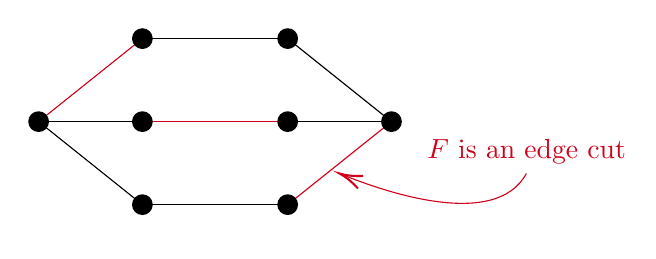
\begin{tikzpicture}[x=0.75pt,y=0.75pt,yscale=-1,xscale=1]
%uncomment if require: \path (0,293); %set diagram left start at 0, and has height of 293

%Straight Lines [id:da05132460204367206] 
\draw [color={rgb, 255:red, 208; green, 2; blue, 27 }  ,draw opacity=1 ][fill={rgb, 255:red, 208; green, 2; blue, 27 }  ,fill opacity=1 ]   (525,135) -- (575,95) ;
%Straight Lines [id:da3882724615712533] 
\draw [color={rgb, 255:red, 208; green, 2; blue, 27 }  ,draw opacity=1 ][fill={rgb, 255:red, 208; green, 2; blue, 27 }  ,fill opacity=1 ]   (455,95) -- (525,95) ;
%Straight Lines [id:da9507618993294427] 
\draw [color={rgb, 255:red, 208; green, 2; blue, 27 }  ,draw opacity=1 ][fill={rgb, 255:red, 208; green, 2; blue, 27 }  ,fill opacity=1 ]   (405,95) -- (455,55) ;
%Shape: Circle [id:dp6621830132982232] 
\draw  [draw opacity=0][fill={rgb, 255:red, 0; green, 0; blue, 0 }  ,fill opacity=1 ] (400,95) .. controls (400,92.24) and (402.24,90) .. (405,90) .. controls (407.76,90) and (410,92.24) .. (410,95) .. controls (410,97.76) and (407.76,100) .. (405,100) .. controls (402.24,100) and (400,97.76) .. (400,95) -- cycle ;
%Straight Lines [id:da4703821448378025] 
\draw [fill={rgb, 255:red, 0; green, 0; blue, 0 }  ,fill opacity=1 ]   (525,55) -- (575,95) ;
%Curve Lines [id:da8935511620092004] 
\draw [color={rgb, 255:red, 208; green, 2; blue, 27 }  ,draw opacity=1 ]   (640,120) .. controls (625.06,147.55) and (570.79,128.43) .. (551.67,120.68) ;
\draw [shift={(550,120)}, rotate = 382.48] [color={rgb, 255:red, 208; green, 2; blue, 27 }  ,draw opacity=1 ][line width=0.75]    (10.93,-3.29) .. controls (6.95,-1.4) and (3.31,-0.3) .. (0,0) .. controls (3.31,0.3) and (6.95,1.4) .. (10.93,3.29)   ;
%Shape: Circle [id:dp13691465882279263] 
\draw  [draw opacity=0][fill={rgb, 255:red, 0; green, 0; blue, 0 }  ,fill opacity=1 ] (450,55) .. controls (450,52.24) and (452.24,50) .. (455,50) .. controls (457.76,50) and (460,52.24) .. (460,55) .. controls (460,57.76) and (457.76,60) .. (455,60) .. controls (452.24,60) and (450,57.76) .. (450,55) -- cycle ;
%Shape: Circle [id:dp17801624792021797] 
\draw  [draw opacity=0][fill={rgb, 255:red, 0; green, 0; blue, 0 }  ,fill opacity=1 ] (450,95) .. controls (450,92.24) and (452.24,90) .. (455,90) .. controls (457.76,90) and (460,92.24) .. (460,95) .. controls (460,97.76) and (457.76,100) .. (455,100) .. controls (452.24,100) and (450,97.76) .. (450,95) -- cycle ;
%Shape: Circle [id:dp48194695736269466] 
\draw  [draw opacity=0][fill={rgb, 255:red, 0; green, 0; blue, 0 }  ,fill opacity=1 ] (450,135) .. controls (450,132.24) and (452.24,130) .. (455,130) .. controls (457.76,130) and (460,132.24) .. (460,135) .. controls (460,137.76) and (457.76,140) .. (455,140) .. controls (452.24,140) and (450,137.76) .. (450,135) -- cycle ;
%Shape: Circle [id:dp5537739143624331] 
\draw  [draw opacity=0][fill={rgb, 255:red, 0; green, 0; blue, 0 }  ,fill opacity=1 ] (520,55) .. controls (520,52.24) and (522.24,50) .. (525,50) .. controls (527.76,50) and (530,52.24) .. (530,55) .. controls (530,57.76) and (527.76,60) .. (525,60) .. controls (522.24,60) and (520,57.76) .. (520,55) -- cycle ;
%Shape: Circle [id:dp6991301367465297] 
\draw  [draw opacity=0][fill={rgb, 255:red, 0; green, 0; blue, 0 }  ,fill opacity=1 ] (520,95) .. controls (520,92.24) and (522.24,90) .. (525,90) .. controls (527.76,90) and (530,92.24) .. (530,95) .. controls (530,97.76) and (527.76,100) .. (525,100) .. controls (522.24,100) and (520,97.76) .. (520,95) -- cycle ;
%Shape: Circle [id:dp35613626441840474] 
\draw  [draw opacity=0][fill={rgb, 255:red, 0; green, 0; blue, 0 }  ,fill opacity=1 ] (520,135) .. controls (520,132.24) and (522.24,130) .. (525,130) .. controls (527.76,130) and (530,132.24) .. (530,135) .. controls (530,137.76) and (527.76,140) .. (525,140) .. controls (522.24,140) and (520,137.76) .. (520,135) -- cycle ;
%Shape: Circle [id:dp10312880289987214] 
\draw  [draw opacity=0][fill={rgb, 255:red, 0; green, 0; blue, 0 }  ,fill opacity=1 ] (570,95) .. controls (570,92.24) and (572.24,90) .. (575,90) .. controls (577.76,90) and (580,92.24) .. (580,95) .. controls (580,97.76) and (577.76,100) .. (575,100) .. controls (572.24,100) and (570,97.76) .. (570,95) -- cycle ;
%Straight Lines [id:da16382674370799444] 
\draw [fill={rgb, 255:red, 0; green, 0; blue, 0 }  ,fill opacity=1 ]   (525,95) -- (575,95) ;
%Straight Lines [id:da5220349317912745] 
\draw [fill={rgb, 255:red, 0; green, 0; blue, 0 }  ,fill opacity=1 ]   (455,55) -- (525,55) ;
%Straight Lines [id:da07426129671663317] 
\draw [fill={rgb, 255:red, 0; green, 0; blue, 0 }  ,fill opacity=1 ]   (455,135) -- (525,135) ;
%Straight Lines [id:da8840713102746135] 
\draw [fill={rgb, 255:red, 0; green, 0; blue, 0 }  ,fill opacity=1 ]   (405,95) -- (455,135) ;
%Straight Lines [id:da0988989789451784] 
\draw [fill={rgb, 255:red, 0; green, 0; blue, 0 }  ,fill opacity=1 ]   (405,95) -- (455,95) ;

% Text Node
\draw (591,102) node [anchor=north west][inner sep=0.75pt]  [color={rgb, 255:red, 208; green, 2; blue, 27 }  ,opacity=1 ] [align=left] {$\displaystyle F$ is an edge cut};


\end{tikzpicture}

\end{center}

\begin{definition}[Cut Edge]
	A \vocab{cut edge} $e \in E$ is an edge so that $G - e$ is disconnected.
\end{definition}
\begin{center}
	

\tikzset{every picture/.style={line width=0.75pt}} %set default line width to 0.75pt        

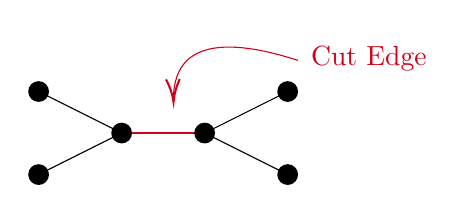
\begin{tikzpicture}[x=0.75pt,y=0.75pt,yscale=-1,xscale=1]
%uncomment if require: \path (0,293); %set diagram left start at 0, and has height of 293

%Shape: Circle [id:dp8102532813420129] 
\draw  [draw opacity=0][fill={rgb, 255:red, 0; green, 0; blue, 0 }  ,fill opacity=1 ] (80,175) .. controls (80,172.24) and (82.24,170) .. (85,170) .. controls (87.76,170) and (90,172.24) .. (90,175) .. controls (90,177.76) and (87.76,180) .. (85,180) .. controls (82.24,180) and (80,177.76) .. (80,175) -- cycle ;
%Shape: Circle [id:dp2488631629694701] 
\draw  [draw opacity=0][fill={rgb, 255:red, 0; green, 0; blue, 0 }  ,fill opacity=1 ] (80,215) .. controls (80,212.24) and (82.24,210) .. (85,210) .. controls (87.76,210) and (90,212.24) .. (90,215) .. controls (90,217.76) and (87.76,220) .. (85,220) .. controls (82.24,220) and (80,217.76) .. (80,215) -- cycle ;
%Shape: Circle [id:dp7720399277074527] 
\draw  [draw opacity=0][fill={rgb, 255:red, 0; green, 0; blue, 0 }  ,fill opacity=1 ] (200,175) .. controls (200,172.24) and (202.24,170) .. (205,170) .. controls (207.76,170) and (210,172.24) .. (210,175) .. controls (210,177.76) and (207.76,180) .. (205,180) .. controls (202.24,180) and (200,177.76) .. (200,175) -- cycle ;
%Shape: Circle [id:dp912532303813462] 
\draw  [draw opacity=0][fill={rgb, 255:red, 0; green, 0; blue, 0 }  ,fill opacity=1 ] (200,215) .. controls (200,212.24) and (202.24,210) .. (205,210) .. controls (207.76,210) and (210,212.24) .. (210,215) .. controls (210,217.76) and (207.76,220) .. (205,220) .. controls (202.24,220) and (200,217.76) .. (200,215) -- cycle ;
%Straight Lines [id:da04015647344399631] 
\draw [fill={rgb, 255:red, 0; green, 0; blue, 0 }  ,fill opacity=1 ]   (85,175) -- (125,195) ;
%Straight Lines [id:da41059919615160323] 
\draw [color={rgb, 255:red, 208; green, 2; blue, 27 }  ,draw opacity=1 ][fill={rgb, 255:red, 0; green, 0; blue, 0 }  ,fill opacity=1 ]   (125,195) -- (165,195) ;
%Straight Lines [id:da45519031183537517] 
\draw [fill={rgb, 255:red, 0; green, 0; blue, 0 }  ,fill opacity=1 ]   (165,195) -- (205,175) ;
%Straight Lines [id:da866450966612112] 
\draw [fill={rgb, 255:red, 0; green, 0; blue, 0 }  ,fill opacity=1 ]   (205,215) -- (165,195) ;
%Straight Lines [id:da32291177428073303] 
\draw [fill={rgb, 255:red, 0; green, 0; blue, 0 }  ,fill opacity=1 ]   (125,195) -- (85,215) ;
%Shape: Circle [id:dp11059613460597517] 
\draw  [draw opacity=0][fill={rgb, 255:red, 0; green, 0; blue, 0 }  ,fill opacity=1 ] (120,195) .. controls (120,192.24) and (122.24,190) .. (125,190) .. controls (127.76,190) and (130,192.24) .. (130,195) .. controls (130,197.76) and (127.76,200) .. (125,200) .. controls (122.24,200) and (120,197.76) .. (120,195) -- cycle ;
%Shape: Circle [id:dp025220046109230565] 
\draw  [draw opacity=0][fill={rgb, 255:red, 0; green, 0; blue, 0 }  ,fill opacity=1 ] (160,195) .. controls (160,192.24) and (162.24,190) .. (165,190) .. controls (167.76,190) and (170,192.24) .. (170,195) .. controls (170,197.76) and (167.76,200) .. (165,200) .. controls (162.24,200) and (160,197.76) .. (160,195) -- cycle ;
%Curve Lines [id:da8282968274627038] 
\draw [color={rgb, 255:red, 208; green, 2; blue, 27 }  ,draw opacity=1 ]   (210,160) .. controls (187.84,152.86) and (150.15,144.5) .. (149.98,178.42) ;
\draw [shift={(150,180)}, rotate = 268.4] [color={rgb, 255:red, 208; green, 2; blue, 27 }  ,draw opacity=1 ][line width=0.75]    (10.93,-3.29) .. controls (6.95,-1.4) and (3.31,-0.3) .. (0,0) .. controls (3.31,0.3) and (6.95,1.4) .. (10.93,3.29)   ;

% Text Node
\draw (215,152) node [anchor=north west][inner sep=0.75pt]  [color={rgb, 255:red, 208; green, 2; blue, 27 }  ,opacity=1 ] [align=left] {Cut Edge};


\end{tikzpicture}
\end{center}

Now similarly to how we had independent paths before (that didn't share vertices), we can define a notion of edge independent paths.

\begin{definition}[Edge Disjoint Paths]
	We say that the $uv$ paths $P_1, \dots, P_k$ are \vocab{edge disjoint} if $E(P_i) \cap E(P_j) = \emptyset$ for all $i \neq j$.
\end{definition}

\begin{center}
	

\tikzset{every picture/.style={line width=0.75pt}} %set default line width to 0.75pt        

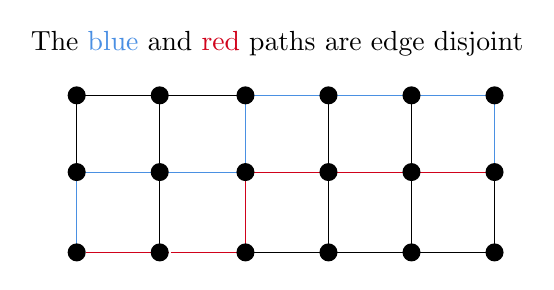
\begin{tikzpicture}[x=0.75pt,y=0.75pt,yscale=-1,xscale=1]
%uncomment if require: \path (0,244); %set diagram left start at 0, and has height of 244

%Straight Lines [id:da6347556786330641] 
\draw [color={rgb, 255:red, 208; green, 2; blue, 27 }  ,draw opacity=1 ]   (245.65,101.31) -- (285.65,101.31) ;
%Straight Lines [id:da9290966267307611] 
\draw [color={rgb, 255:red, 208; green, 2; blue, 27 }  ,draw opacity=1 ]   (88.69,140) -- (128.69,140) ;
%Straight Lines [id:da06230159780920708] 
\draw [color={rgb, 255:red, 208; green, 2; blue, 27 }  ,draw opacity=1 ]   (130,140) -- (170,140) ;
%Straight Lines [id:da14619845565883882] 
\draw    (165.65,140) -- (205.65,140) ;
%Straight Lines [id:da7599531000299461] 
\draw    (205.65,140) -- (245.65,140) ;
%Straight Lines [id:da4416422418458743] 
\draw    (245.65,140) -- (285.65,140) ;
%Straight Lines [id:da699256527441075] 
\draw [color={rgb, 255:red, 74; green, 144; blue, 226 }  ,draw opacity=1 ]   (84.35,101.31) -- (124.35,101.31) ;
%Straight Lines [id:da4575003368976278] 
\draw [color={rgb, 255:red, 74; green, 144; blue, 226 }  ,draw opacity=1 ]   (125.65,101.31) -- (165.65,101.31) ;
%Straight Lines [id:da24796604604910966] 
\draw [color={rgb, 255:red, 208; green, 2; blue, 27 }  ,draw opacity=1 ]   (170,101.31) -- (210,101.31) ;
%Straight Lines [id:da8487454519232515] 
\draw [color={rgb, 255:red, 208; green, 2; blue, 27 }  ,draw opacity=1 ]   (210,101.31) -- (250,101.31) ;
%Straight Lines [id:da15403754197143482] 
\draw [color={rgb, 255:red, 74; green, 144; blue, 226 }  ,draw opacity=1 ]   (84.35,101.31) -- (84.35,140) ;
%Straight Lines [id:da8200994215251722] 
\draw    (124.35,101.31) -- (124.35,140) ;
%Straight Lines [id:da3241050601262073] 
\draw [color={rgb, 255:red, 208; green, 2; blue, 27 }  ,draw opacity=1 ]   (165.65,101.31) -- (165.65,140) ;
%Straight Lines [id:da0706763748096414] 
\draw    (205.65,101.31) -- (205.65,140) ;
%Straight Lines [id:da4617888693593192] 
\draw    (245.65,101.31) -- (245.65,140) ;
%Straight Lines [id:da0493845533381565] 
\draw    (285.65,101.31) -- (285.65,140) ;
%Straight Lines [id:da6732846881927783] 
\draw    (84.35,64.35) -- (124.35,64.35) ;
%Straight Lines [id:da9472691742802231] 
\draw    (125.65,64.35) -- (165.65,64.35) ;
%Straight Lines [id:da940002891500757] 
\draw [color={rgb, 255:red, 74; green, 144; blue, 226 }  ,draw opacity=1 ]   (165.65,64.35) -- (205.65,64.35) ;
%Straight Lines [id:da9244457293063586] 
\draw [color={rgb, 255:red, 74; green, 144; blue, 226 }  ,draw opacity=1 ]   (205.65,64.35) -- (245.65,64.35) ;
%Straight Lines [id:da5841783890669372] 
\draw [color={rgb, 255:red, 74; green, 144; blue, 226 }  ,draw opacity=1 ]   (245.65,64.35) -- (285.65,64.35) ;
%Straight Lines [id:da7634050489694235] 
\draw    (84.35,64.35) -- (84.35,103.04) ;
%Straight Lines [id:da4469282654312059] 
\draw    (124.35,64.35) -- (124.35,103.04) ;
%Straight Lines [id:da9528312169124284] 
\draw [color={rgb, 255:red, 74; green, 144; blue, 226 }  ,draw opacity=1 ]   (165.65,64.35) -- (165.65,103.04) ;
%Straight Lines [id:da5425355624782201] 
\draw    (205.65,64.35) -- (205.65,103.04) ;
%Straight Lines [id:da9916166101902055] 
\draw    (245.65,64.35) -- (245.65,103.04) ;
%Straight Lines [id:da5987936422359369] 
\draw [color={rgb, 255:red, 74; green, 144; blue, 226 }  ,draw opacity=1 ]   (285.65,64.35) -- (285.65,103.04) ;
%Shape: Ellipse [id:dp47720978935459246] 
\draw  [draw opacity=0][fill={rgb, 255:red, 0; green, 0; blue, 0 }  ,fill opacity=1 ] (80,140) .. controls (80,137.6) and (81.95,135.65) .. (84.35,135.65) .. controls (86.74,135.65) and (88.69,137.6) .. (88.69,140) .. controls (88.69,142.4) and (86.74,144.35) .. (84.35,144.35) .. controls (81.95,144.35) and (80,142.4) .. (80,140) -- cycle ;
%Shape: Ellipse [id:dp34028922037404286] 
\draw  [draw opacity=0][fill={rgb, 255:red, 0; green, 0; blue, 0 }  ,fill opacity=1 ] (120,140) .. controls (120,137.6) and (121.95,135.65) .. (124.35,135.65) .. controls (126.74,135.65) and (128.69,137.6) .. (128.69,140) .. controls (128.69,142.4) and (126.74,144.35) .. (124.35,144.35) .. controls (121.95,144.35) and (120,142.4) .. (120,140) -- cycle ;
%Shape: Ellipse [id:dp6653845429944741] 
\draw  [draw opacity=0][fill={rgb, 255:red, 0; green, 0; blue, 0 }  ,fill opacity=1 ] (201.31,140) .. controls (201.31,137.6) and (203.26,135.65) .. (205.65,135.65) .. controls (208.05,135.65) and (210,137.6) .. (210,140) .. controls (210,142.4) and (208.05,144.35) .. (205.65,144.35) .. controls (203.26,144.35) and (201.31,142.4) .. (201.31,140) -- cycle ;
%Shape: Ellipse [id:dp7096288086795957] 
\draw  [draw opacity=0][fill={rgb, 255:red, 0; green, 0; blue, 0 }  ,fill opacity=1 ] (241.31,140) .. controls (241.31,137.6) and (243.26,135.65) .. (245.65,135.65) .. controls (248.05,135.65) and (250,137.6) .. (250,140) .. controls (250,142.4) and (248.05,144.35) .. (245.65,144.35) .. controls (243.26,144.35) and (241.31,142.4) .. (241.31,140) -- cycle ;
%Shape: Ellipse [id:dp2929245397228538] 
\draw  [draw opacity=0][fill={rgb, 255:red, 0; green, 0; blue, 0 }  ,fill opacity=1 ] (120,101.31) .. controls (120,98.91) and (121.95,96.96) .. (124.35,96.96) .. controls (126.74,96.96) and (128.69,98.91) .. (128.69,101.31) .. controls (128.69,103.71) and (126.74,105.65) .. (124.35,105.65) .. controls (121.95,105.65) and (120,103.71) .. (120,101.31) -- cycle ;
%Shape: Ellipse [id:dp173232717283752] 
\draw  [draw opacity=0][fill={rgb, 255:red, 0; green, 0; blue, 0 }  ,fill opacity=1 ] (201.31,101.31) .. controls (201.31,98.91) and (203.26,96.96) .. (205.65,96.96) .. controls (208.05,96.96) and (210,98.91) .. (210,101.31) .. controls (210,103.71) and (208.05,105.65) .. (205.65,105.65) .. controls (203.26,105.65) and (201.31,103.71) .. (201.31,101.31) -- cycle ;
%Shape: Ellipse [id:dp3427062902743854] 
\draw  [draw opacity=0][fill={rgb, 255:red, 0; green, 0; blue, 0 }  ,fill opacity=1 ] (241.31,101.31) .. controls (241.31,98.91) and (243.26,96.96) .. (245.65,96.96) .. controls (248.05,96.96) and (250,98.91) .. (250,101.31) .. controls (250,103.71) and (248.05,105.65) .. (245.65,105.65) .. controls (243.26,105.65) and (241.31,103.71) .. (241.31,101.31) -- cycle ;
%Shape: Ellipse [id:dp9904804519495449] 
\draw  [draw opacity=0][fill={rgb, 255:red, 0; green, 0; blue, 0 }  ,fill opacity=1 ] (281.31,101.31) .. controls (281.31,98.91) and (283.26,96.96) .. (285.65,96.96) .. controls (288.05,96.96) and (290,98.91) .. (290,101.31) .. controls (290,103.71) and (288.05,105.65) .. (285.65,105.65) .. controls (283.26,105.65) and (281.31,103.71) .. (281.31,101.31) -- cycle ;
%Shape: Ellipse [id:dp4075695180070539] 
\draw  [draw opacity=0][fill={rgb, 255:red, 0; green, 0; blue, 0 }  ,fill opacity=1 ] (80,101.31) .. controls (80,98.91) and (81.95,96.96) .. (84.35,96.96) .. controls (86.74,96.96) and (88.69,98.91) .. (88.69,101.31) .. controls (88.69,103.71) and (86.74,105.65) .. (84.35,105.65) .. controls (81.95,105.65) and (80,103.71) .. (80,101.31) -- cycle ;
%Shape: Ellipse [id:dp349638513362311] 
\draw  [draw opacity=0][fill={rgb, 255:red, 0; green, 0; blue, 0 }  ,fill opacity=1 ] (281.31,140) .. controls (281.31,137.6) and (283.26,135.65) .. (285.65,135.65) .. controls (288.05,135.65) and (290,137.6) .. (290,140) .. controls (290,142.4) and (288.05,144.35) .. (285.65,144.35) .. controls (283.26,144.35) and (281.31,142.4) .. (281.31,140) -- cycle ;
%Shape: Ellipse [id:dp7824695613705636] 
\draw  [draw opacity=0][fill={rgb, 255:red, 0; green, 0; blue, 0 }  ,fill opacity=1 ] (161.31,140) .. controls (161.31,137.6) and (163.26,135.65) .. (165.65,135.65) .. controls (168.05,135.65) and (170,137.6) .. (170,140) .. controls (170,142.4) and (168.05,144.35) .. (165.65,144.35) .. controls (163.26,144.35) and (161.31,142.4) .. (161.31,140) -- cycle ;
%Shape: Ellipse [id:dp9207984667944648] 
\draw  [draw opacity=0][fill={rgb, 255:red, 0; green, 0; blue, 0 }  ,fill opacity=1 ] (161.31,101.31) .. controls (161.31,98.91) and (163.26,96.96) .. (165.65,96.96) .. controls (168.05,96.96) and (170,98.91) .. (170,101.31) .. controls (170,103.71) and (168.05,105.65) .. (165.65,105.65) .. controls (163.26,105.65) and (161.31,103.71) .. (161.31,101.31) -- cycle ;
%Shape: Ellipse [id:dp30033713653444905] 
\draw  [draw opacity=0][fill={rgb, 255:red, 0; green, 0; blue, 0 }  ,fill opacity=1 ] (120,64.35) .. controls (120,61.95) and (121.95,60) .. (124.35,60) .. controls (126.74,60) and (128.69,61.95) .. (128.69,64.35) .. controls (128.69,66.74) and (126.74,68.69) .. (124.35,68.69) .. controls (121.95,68.69) and (120,66.74) .. (120,64.35) -- cycle ;
%Shape: Ellipse [id:dp02071524541501979] 
\draw  [draw opacity=0][fill={rgb, 255:red, 0; green, 0; blue, 0 }  ,fill opacity=1 ] (201.31,64.35) .. controls (201.31,61.95) and (203.26,60) .. (205.65,60) .. controls (208.05,60) and (210,61.95) .. (210,64.35) .. controls (210,66.74) and (208.05,68.69) .. (205.65,68.69) .. controls (203.26,68.69) and (201.31,66.74) .. (201.31,64.35) -- cycle ;
%Shape: Ellipse [id:dp8556926842820846] 
\draw  [draw opacity=0][fill={rgb, 255:red, 0; green, 0; blue, 0 }  ,fill opacity=1 ] (241.31,64.35) .. controls (241.31,61.95) and (243.26,60) .. (245.65,60) .. controls (248.05,60) and (250,61.95) .. (250,64.35) .. controls (250,66.74) and (248.05,68.69) .. (245.65,68.69) .. controls (243.26,68.69) and (241.31,66.74) .. (241.31,64.35) -- cycle ;
%Shape: Ellipse [id:dp8264738305184547] 
\draw  [draw opacity=0][fill={rgb, 255:red, 0; green, 0; blue, 0 }  ,fill opacity=1 ] (281.31,64.35) .. controls (281.31,61.95) and (283.26,60) .. (285.65,60) .. controls (288.05,60) and (290,61.95) .. (290,64.35) .. controls (290,66.74) and (288.05,68.69) .. (285.65,68.69) .. controls (283.26,68.69) and (281.31,66.74) .. (281.31,64.35) -- cycle ;
%Shape: Ellipse [id:dp5721413351762408] 
\draw  [draw opacity=0][fill={rgb, 255:red, 0; green, 0; blue, 0 }  ,fill opacity=1 ] (80,64.35) .. controls (80,61.95) and (81.95,60) .. (84.35,60) .. controls (86.74,60) and (88.69,61.95) .. (88.69,64.35) .. controls (88.69,66.74) and (86.74,68.69) .. (84.35,68.69) .. controls (81.95,68.69) and (80,66.74) .. (80,64.35) -- cycle ;
%Shape: Ellipse [id:dp3322071843175737] 
\draw  [draw opacity=0][fill={rgb, 255:red, 0; green, 0; blue, 0 }  ,fill opacity=1 ] (161.31,64.35) .. controls (161.31,61.95) and (163.26,60) .. (165.65,60) .. controls (168.05,60) and (170,61.95) .. (170,64.35) .. controls (170,66.74) and (168.05,68.69) .. (165.65,68.69) .. controls (163.26,68.69) and (161.31,66.74) .. (161.31,64.35) -- cycle ;

% Text Node
\draw (61,32) node [anchor=north west][inner sep=0.75pt]   [align=left] {The \textcolor[rgb]{0.29,0.56,0.89}{blue} and \textcolor[rgb]{0.82,0.01,0.11}{red} paths are edge disjoint};


\end{tikzpicture}

\end{center}

We can then define edge connectivity (our deletion notion).

\begin{definition}[Edge Connectivity]
	Define the \vocab{edge connectivity} of $G$, $\lambda(G)$ to be the smallest $|S|$ with $S \subseteq E$ such that $G - S$ is disconnected.
\end{definition}
\begin{definition}[$k$-Edge-Connected]
	We say a graph $G$ is \vocab{$k$-edge-connected} if $\lambda(G) \geq k$. In other words, $G - F$ is connected for all $|F|\leq k - 1$, with $F \subseteq E$. 
\end{definition}

We note that $G$ is 1-edge-connected if and only if it is connected, and it is 2-edge-connected if and only if there is no cut edge.

We have a Menger's theorem for this notion of connectivity also.

\begin{theorem}[Menger's Theorem, Edge Version]
	Let $G = (V, E)$ be a graph, and $u, v$ be distinct vertices of $G$. If every set of edges $F \subseteq E$ that separates $u$ from $v$ has size greater than or equal to $k$, then there exists $k$ edge disjoint paths from $u$ to $v$.
\end{theorem}

We also have a similar second version.

\begin{theorem}[Menger's Theorem, Edge Version Two]
Let $G = (V, E)$ be a graph. Then $G$ is $k$-edge-connected if and only if for every $u, v \in V$ with $u \neq v$ there exists $k$ edge disjoint $uv$-paths $P_1, \dots, P_k$.
\end{theorem}

We are going to prove this by constructing a graph that we can then get the required result from my applying vertex Menger. The construction will be based on the idea of a \emph{line graph}.

\begin{definition}[Line Graph]
	Given a graph $G = (V, E)$, we define $L(G)$ to be the \vocab{line graph} as follows.
	$V(L(G)) = E$, and for $e, f \in E$, we have $ef \in E(L(G))$ if $e \cap f \neq \emptyset$.
\end{definition}

An example of a graph and its corresponding line graph is shown below.
\begin{center}
	

\tikzset{every picture/.style={line width=0.75pt}} %set default line width to 0.75pt        

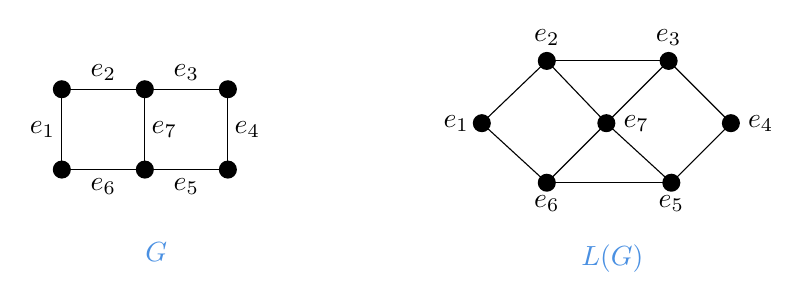
\begin{tikzpicture}[x=0.75pt,y=0.75pt,yscale=-1,xscale=1]
%uncomment if require: \path (0,244); %set diagram left start at 0, and has height of 244

%Shape: Ellipse [id:dp6428003664164491] 
\draw  [draw opacity=0][fill={rgb, 255:red, 0; green, 0; blue, 0 }  ,fill opacity=1 ] (147.65,138) .. controls (147.65,135.6) and (149.6,133.65) .. (152,133.65) .. controls (154.4,133.65) and (156.35,135.6) .. (156.35,138) .. controls (156.35,140.4) and (154.4,142.35) .. (152,142.35) .. controls (149.6,142.35) and (147.65,140.4) .. (147.65,138) -- cycle ;
%Straight Lines [id:da7030202286088147] 
\draw    (152,138) -- (192,138) ;
%Shape: Ellipse [id:dp17395821646954623] 
\draw  [draw opacity=0][fill={rgb, 255:red, 0; green, 0; blue, 0 }  ,fill opacity=1 ] (187.65,138) .. controls (187.65,135.6) and (189.6,133.65) .. (192,133.65) .. controls (194.4,133.65) and (196.35,135.6) .. (196.35,138) .. controls (196.35,140.4) and (194.4,142.35) .. (192,142.35) .. controls (189.6,142.35) and (187.65,140.4) .. (187.65,138) -- cycle ;
%Straight Lines [id:da6079106266944129] 
\draw    (192,138) -- (232,138) ;
%Shape: Ellipse [id:dp2557134341164947] 
\draw  [draw opacity=0][fill={rgb, 255:red, 0; green, 0; blue, 0 }  ,fill opacity=1 ] (147.65,99.31) .. controls (147.65,96.91) and (149.6,94.96) .. (152,94.96) .. controls (154.4,94.96) and (156.35,96.91) .. (156.35,99.31) .. controls (156.35,101.71) and (154.4,103.65) .. (152,103.65) .. controls (149.6,103.65) and (147.65,101.71) .. (147.65,99.31) -- cycle ;
%Straight Lines [id:da9358493211756559] 
\draw    (152,99.31) -- (192,99.31) ;
%Shape: Ellipse [id:dp44140773078706885] 
\draw  [draw opacity=0][fill={rgb, 255:red, 0; green, 0; blue, 0 }  ,fill opacity=1 ] (187.65,99.31) .. controls (187.65,96.91) and (189.6,94.96) .. (192,94.96) .. controls (194.4,94.96) and (196.35,96.91) .. (196.35,99.31) .. controls (196.35,101.71) and (194.4,103.65) .. (192,103.65) .. controls (189.6,103.65) and (187.65,101.71) .. (187.65,99.31) -- cycle ;
%Straight Lines [id:da3545617009384612] 
\draw    (192,99.31) -- (232,99.31) ;
%Shape: Ellipse [id:dp9082475723239443] 
\draw  [draw opacity=0][fill={rgb, 255:red, 0; green, 0; blue, 0 }  ,fill opacity=1 ] (227.65,99.31) .. controls (227.65,96.91) and (229.6,94.96) .. (232,94.96) .. controls (234.4,94.96) and (236.35,96.91) .. (236.35,99.31) .. controls (236.35,101.71) and (234.4,103.65) .. (232,103.65) .. controls (229.6,103.65) and (227.65,101.71) .. (227.65,99.31) -- cycle ;
%Straight Lines [id:da3386382981491318] 
\draw    (152,99.31) -- (152,138) ;
%Straight Lines [id:da9245301218270087] 
\draw    (192,99.31) -- (192,138) ;
%Straight Lines [id:da40680137070767797] 
\draw    (232,99.31) -- (232,138) ;
%Shape: Ellipse [id:dp5370665255767365] 
\draw  [draw opacity=0][fill={rgb, 255:red, 0; green, 0; blue, 0 }  ,fill opacity=1 ] (227.65,138) .. controls (227.65,135.6) and (229.6,133.65) .. (232,133.65) .. controls (234.4,133.65) and (236.35,135.6) .. (236.35,138) .. controls (236.35,140.4) and (234.4,142.35) .. (232,142.35) .. controls (229.6,142.35) and (227.65,140.4) .. (227.65,138) -- cycle ;
%Shape: Ellipse [id:dp3486272594619664] 
\draw  [draw opacity=0][fill={rgb, 255:red, 0; green, 0; blue, 0 }  ,fill opacity=1 ] (350,115.65) .. controls (350,113.26) and (351.95,111.31) .. (354.35,111.31) .. controls (356.74,111.31) and (358.69,113.26) .. (358.69,115.65) .. controls (358.69,118.05) and (356.74,120) .. (354.35,120) .. controls (351.95,120) and (350,118.05) .. (350,115.65) -- cycle ;
%Shape: Ellipse [id:dp894692337544137] 
\draw  [draw opacity=0][fill={rgb, 255:red, 0; green, 0; blue, 0 }  ,fill opacity=1 ] (410,115.65) .. controls (410,113.26) and (411.95,111.31) .. (414.35,111.31) .. controls (416.74,111.31) and (418.69,113.26) .. (418.69,115.65) .. controls (418.69,118.05) and (416.74,120) .. (414.35,120) .. controls (411.95,120) and (410,118.05) .. (410,115.65) -- cycle ;
%Shape: Ellipse [id:dp9775853706047504] 
\draw  [draw opacity=0][fill={rgb, 255:red, 0; green, 0; blue, 0 }  ,fill opacity=1 ] (470,115.65) .. controls (470,113.26) and (471.95,111.31) .. (474.35,111.31) .. controls (476.74,111.31) and (478.69,113.26) .. (478.69,115.65) .. controls (478.69,118.05) and (476.74,120) .. (474.35,120) .. controls (471.95,120) and (470,118.05) .. (470,115.65) -- cycle ;
%Shape: Ellipse [id:dp4675924367631904] 
\draw  [draw opacity=0][fill={rgb, 255:red, 0; green, 0; blue, 0 }  ,fill opacity=1 ] (381.31,85.65) .. controls (381.31,83.26) and (383.26,81.31) .. (385.65,81.31) .. controls (388.05,81.31) and (390,83.26) .. (390,85.65) .. controls (390,88.05) and (388.05,90) .. (385.65,90) .. controls (383.26,90) and (381.31,88.05) .. (381.31,85.65) -- cycle ;
%Shape: Ellipse [id:dp7821466043254435] 
\draw  [draw opacity=0][fill={rgb, 255:red, 0; green, 0; blue, 0 }  ,fill opacity=1 ] (440,85.65) .. controls (440,83.26) and (441.95,81.31) .. (444.35,81.31) .. controls (446.74,81.31) and (448.69,83.26) .. (448.69,85.65) .. controls (448.69,88.05) and (446.74,90) .. (444.35,90) .. controls (441.95,90) and (440,88.05) .. (440,85.65) -- cycle ;
%Shape: Ellipse [id:dp5985312808923524] 
\draw  [draw opacity=0][fill={rgb, 255:red, 0; green, 0; blue, 0 }  ,fill opacity=1 ] (381.31,144.35) .. controls (381.31,141.95) and (383.26,140) .. (385.65,140) .. controls (388.05,140) and (390,141.95) .. (390,144.35) .. controls (390,146.74) and (388.05,148.69) .. (385.65,148.69) .. controls (383.26,148.69) and (381.31,146.74) .. (381.31,144.35) -- cycle ;
%Shape: Ellipse [id:dp48445315814132495] 
\draw  [draw opacity=0][fill={rgb, 255:red, 0; green, 0; blue, 0 }  ,fill opacity=1 ] (441.31,144.35) .. controls (441.31,141.95) and (443.26,140) .. (445.65,140) .. controls (448.05,140) and (450,141.95) .. (450,144.35) .. controls (450,146.74) and (448.05,148.69) .. (445.65,148.69) .. controls (443.26,148.69) and (441.31,146.74) .. (441.31,144.35) -- cycle ;
%Straight Lines [id:da6298910966381643] 
\draw    (354.35,115.65) -- (385.65,85.65) ;
%Straight Lines [id:da821550086240479] 
\draw    (385.65,85.65) -- (444.35,85.65) ;
%Straight Lines [id:da8468741650070947] 
\draw    (474.35,115.65) -- (444.35,85.65) ;
%Straight Lines [id:da4151696963649193] 
\draw    (474.35,115.65) -- (445.65,144.35) ;
%Straight Lines [id:da45993932440690843] 
\draw    (444.35,85.65) -- (414.35,115.65) ;
%Straight Lines [id:da8501014042740391] 
\draw    (445.65,144.35) -- (385.65,144.35) ;
%Straight Lines [id:da8864999112992344] 
\draw    (385.65,144.35) -- (354.35,115.65) ;
%Straight Lines [id:da09669477773207658] 
\draw    (414.35,115.65) -- (385.65,85.65) ;
%Straight Lines [id:da1680105672865213] 
\draw    (445.65,144.35) -- (414.35,115.65) ;
%Straight Lines [id:da1300989892856761] 
\draw    (385.65,144.35) -- (414.35,115.65) ;

% Text Node
\draw (150,118.65) node [anchor=east] [inner sep=0.75pt]  [color={rgb, 255:red, 0; green, 0; blue, 0 }  ,opacity=1 ]  {$e_{1}$};
% Text Node
\draw (172,96.31) node [anchor=south] [inner sep=0.75pt]  [color={rgb, 255:red, 0; green, 0; blue, 0 }  ,opacity=1 ]  {$e_{2}$};
% Text Node
\draw (212,96.31) node [anchor=south] [inner sep=0.75pt]  [color={rgb, 255:red, 0; green, 0; blue, 0 }  ,opacity=1 ]  {$e_{3}$};
% Text Node
\draw (234,118.65) node [anchor=west] [inner sep=0.75pt]  [color={rgb, 255:red, 0; green, 0; blue, 0 }  ,opacity=1 ]  {$e_{4}$};
% Text Node
\draw (194,118.65) node [anchor=west] [inner sep=0.75pt]  [color={rgb, 255:red, 0; green, 0; blue, 0 }  ,opacity=1 ]  {$e_{7}$};
% Text Node
\draw (212,141) node [anchor=north] [inner sep=0.75pt]  [color={rgb, 255:red, 0; green, 0; blue, 0 }  ,opacity=1 ]  {$e_{5}$};
% Text Node
\draw (172,141) node [anchor=north] [inner sep=0.75pt]  [color={rgb, 255:red, 0; green, 0; blue, 0 }  ,opacity=1 ]  {$e_{6}$};
% Text Node
\draw (349.35,115.65) node [anchor=east] [inner sep=0.75pt]  [color={rgb, 255:red, 0; green, 0; blue, 0 }  ,opacity=1 ]  {$e_{1}$};
% Text Node
\draw (385.65,79.65) node [anchor=south] [inner sep=0.75pt]  [color={rgb, 255:red, 0; green, 0; blue, 0 }  ,opacity=1 ]  {$e_{2}$};
% Text Node
\draw (444.35,79.65) node [anchor=south] [inner sep=0.75pt]  [color={rgb, 255:red, 0; green, 0; blue, 0 }  ,opacity=1 ]  {$e_{3}$};
% Text Node
\draw (385.65,149.35) node [anchor=north] [inner sep=0.75pt]  [color={rgb, 255:red, 0; green, 0; blue, 0 }  ,opacity=1 ]  {$e_{6}$};
% Text Node
\draw (445.65,149.35) node [anchor=north] [inner sep=0.75pt]  [color={rgb, 255:red, 0; green, 0; blue, 0 }  ,opacity=1 ]  {$e_{5}$};
% Text Node
\draw (481.35,115.65) node [anchor=west] [inner sep=0.75pt]  [color={rgb, 255:red, 0; green, 0; blue, 0 }  ,opacity=1 ]  {$e_{4}$};
% Text Node
\draw (421.35,115.65) node [anchor=west] [inner sep=0.75pt]  [color={rgb, 255:red, 0; green, 0; blue, 0 }  ,opacity=1 ]  {$e_{7}$};
% Text Node
\draw (191,172) node [anchor=north west][inner sep=0.75pt]  [color={rgb, 255:red, 74; green, 144; blue, 226 }  ,opacity=1 ]  {$G$};
% Text Node
\draw (401,173) node [anchor=north west][inner sep=0.75pt]  [color={rgb, 255:red, 74; green, 144; blue, 226 }  ,opacity=1 ]  {$L( G)$};


\end{tikzpicture}

\end{center}
We can now prove the edge version of Menger's theorem.

\begin{proof}[Proof (Menger's Theorem, Edge Version)]
	We are given a graph $G = (V, E)$ and distinct vertices $u, v \in V$ such that every $u, v$ separator has size $\geq k$.

	Construct the graph $\tilde{G}$ which is $L(G)$ along with vertices $u$ and $v$ with $u$ joined to all $e \in V(L(G))$ such that $u \in e$, and likewise for $v$.

	Then applying Menger's theorem (the vertex version, form one) to $\tilde{G}$ with $u, v$ as the distinguished vertices.
\end{proof}

\section{Planar Graphs}

Informally, a graph is \vocab{planar} if
it can be drawn in the plane without any pair of edges crossing.

For example the cube graph we mentioned earlier is planar, as we can draw it as below.

\begin{center}
	

\tikzset{every picture/.style={line width=0.75pt}} %set default line width to 0.75pt        

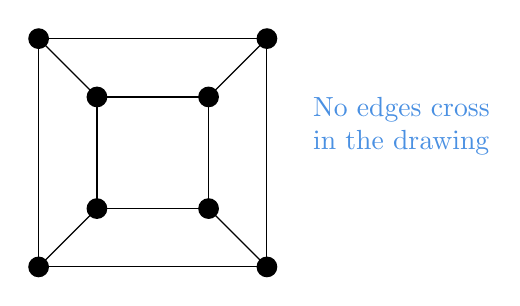
\begin{tikzpicture}[x=0.75pt,y=0.75pt,yscale=-1,xscale=1]
%uncomment if require: \path (0,193); %set diagram left start at 0, and has height of 193

%Shape: Bevel [id:dp9129878220464666] 
\draw   (235,45) -- (345,45) -- (345,155) -- (235,155) -- cycle ; \draw   (263.11,73.11) -- (316.89,73.11) -- (316.89,126.89) -- (263.11,126.89) -- cycle ; \draw   (235,45) -- (263.11,73.11) ; \draw   (345,45) -- (316.89,73.11) ; \draw   (345,155) -- (316.89,126.89) ; \draw   (235,155) -- (263.11,126.89) ;
%Shape: Circle [id:dp6335541713411533] 
\draw  [draw opacity=0][fill={rgb, 255:red, 0; green, 0; blue, 0 }  ,fill opacity=1 ] (230,45) .. controls (230,42.24) and (232.24,40) .. (235,40) .. controls (237.76,40) and (240,42.24) .. (240,45) .. controls (240,47.76) and (237.76,50) .. (235,50) .. controls (232.24,50) and (230,47.76) .. (230,45) -- cycle ;
%Shape: Circle [id:dp3366684932480821] 
\draw  [draw opacity=0][fill={rgb, 255:red, 0; green, 0; blue, 0 }  ,fill opacity=1 ] (258.11,73.11) .. controls (258.11,70.35) and (260.35,68.11) .. (263.11,68.11) .. controls (265.87,68.11) and (268.11,70.35) .. (268.11,73.11) .. controls (268.11,75.87) and (265.87,78.11) .. (263.11,78.11) .. controls (260.35,78.11) and (258.11,75.87) .. (258.11,73.11) -- cycle ;
%Shape: Circle [id:dp9091812925824844] 
\draw  [draw opacity=0][fill={rgb, 255:red, 0; green, 0; blue, 0 }  ,fill opacity=1 ] (311.89,73.11) .. controls (311.89,70.35) and (314.13,68.11) .. (316.89,68.11) .. controls (319.65,68.11) and (321.89,70.35) .. (321.89,73.11) .. controls (321.89,75.87) and (319.65,78.11) .. (316.89,78.11) .. controls (314.13,78.11) and (311.89,75.87) .. (311.89,73.11) -- cycle ;
%Shape: Circle [id:dp40413958574242004] 
\draw  [draw opacity=0][fill={rgb, 255:red, 0; green, 0; blue, 0 }  ,fill opacity=1 ] (340,45) .. controls (340,42.24) and (342.24,40) .. (345,40) .. controls (347.76,40) and (350,42.24) .. (350,45) .. controls (350,47.76) and (347.76,50) .. (345,50) .. controls (342.24,50) and (340,47.76) .. (340,45) -- cycle ;
%Shape: Circle [id:dp20893509275923838] 
\draw  [draw opacity=0][fill={rgb, 255:red, 0; green, 0; blue, 0 }  ,fill opacity=1 ] (340,155) .. controls (340,152.24) and (342.24,150) .. (345,150) .. controls (347.76,150) and (350,152.24) .. (350,155) .. controls (350,157.76) and (347.76,160) .. (345,160) .. controls (342.24,160) and (340,157.76) .. (340,155) -- cycle ;
%Shape: Circle [id:dp7001792293163452] 
\draw  [draw opacity=0][fill={rgb, 255:red, 0; green, 0; blue, 0 }  ,fill opacity=1 ] (311.89,126.89) .. controls (311.89,124.13) and (314.13,121.89) .. (316.89,121.89) .. controls (319.65,121.89) and (321.89,124.13) .. (321.89,126.89) .. controls (321.89,129.65) and (319.65,131.89) .. (316.89,131.89) .. controls (314.13,131.89) and (311.89,129.65) .. (311.89,126.89) -- cycle ;
%Shape: Circle [id:dp5505232094882361] 
\draw  [draw opacity=0][fill={rgb, 255:red, 0; green, 0; blue, 0 }  ,fill opacity=1 ] (258.11,126.89) .. controls (258.11,124.13) and (260.35,121.89) .. (263.11,121.89) .. controls (265.87,121.89) and (268.11,124.13) .. (268.11,126.89) .. controls (268.11,129.65) and (265.87,131.89) .. (263.11,131.89) .. controls (260.35,131.89) and (258.11,129.65) .. (258.11,126.89) -- cycle ;
%Shape: Circle [id:dp46900957197335613] 
\draw  [draw opacity=0][fill={rgb, 255:red, 0; green, 0; blue, 0 }  ,fill opacity=1 ] (230,155) .. controls (230,152.24) and (232.24,150) .. (235,150) .. controls (237.76,150) and (240,152.24) .. (240,155) .. controls (240,157.76) and (237.76,160) .. (235,160) .. controls (232.24,160) and (230,157.76) .. (230,155) -- cycle ;

% Text Node
\draw (366,72) node [anchor=north west][inner sep=0.75pt]  [color={rgb, 255:red, 74; green, 144; blue, 226 }  ,opacity=1 ] [align=left] {No edges cross\\in the drawing};


\end{tikzpicture}

\end{center}

Of course, a graph is planar only if \emph{there is some drawing} where the edges don't intersect. For example, we could draw the cube graph as below (where edges intersect), and the graph would still be planar.

\begin{center}
	

\tikzset{every picture/.style={line width=0.75pt}} %set default line width to 0.75pt        

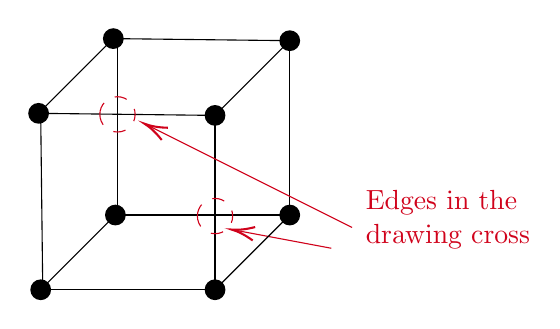
\begin{tikzpicture}[x=0.75pt,y=0.75pt,yscale=-1,xscale=1]
%uncomment if require: \path (0,300); %set diagram left start at 0, and has height of 300

%Straight Lines [id:da7277052618541983] 
\draw [color={rgb, 255:red, 0; green, 0; blue, 0 }  ,draw opacity=1 ]   (146,75) -- (146,159) ;
%Straight Lines [id:da5324681155522419] 
\draw [color={rgb, 255:red, 0; green, 0; blue, 0 }  ,draw opacity=1 ]   (193,111) -- (193,195) ;
%Straight Lines [id:da6044013070050044] 
\draw [color={rgb, 255:red, 0; green, 0; blue, 0 }  ,draw opacity=1 ]   (229,75) -- (229,159) ;
%Straight Lines [id:da824112102193613] 
\draw [color={rgb, 255:red, 0; green, 0; blue, 0 }  ,draw opacity=1 ]   (110,195) -- (109,110) ;
%Straight Lines [id:da5782521272515242] 
\draw    (229,159) -- (145,159) ;
%Straight Lines [id:da37550118016679224] 
\draw    (109,195) -- (145,159) ;
%Straight Lines [id:da21885833636849117] 
\draw [color={rgb, 255:red, 208; green, 2; blue, 27 }  ,draw opacity=1 ]   (249,175) -- (202.97,166.37) ;
\draw [shift={(201,166)}, rotate = 370.62] [color={rgb, 255:red, 208; green, 2; blue, 27 }  ,draw opacity=1 ][line width=0.75]    (10.93,-3.29) .. controls (6.95,-1.4) and (3.31,-0.3) .. (0,0) .. controls (3.31,0.3) and (6.95,1.4) .. (10.93,3.29)   ;
%Shape: Circle [id:dp9660990604637021] 
\draw  [draw opacity=0][fill={rgb, 255:red, 0; green, 0; blue, 0 }  ,fill opacity=1 ] (104,195) .. controls (104,192.24) and (106.24,190) .. (109,190) .. controls (111.76,190) and (114,192.24) .. (114,195) .. controls (114,197.76) and (111.76,200) .. (109,200) .. controls (106.24,200) and (104,197.76) .. (104,195) -- cycle ;
%Shape: Circle [id:dp033431923041256084] 
\draw  [draw opacity=0][fill={rgb, 255:red, 0; green, 0; blue, 0 }  ,fill opacity=1 ] (188,195) .. controls (188,192.24) and (190.24,190) .. (193,190) .. controls (195.76,190) and (198,192.24) .. (198,195) .. controls (198,197.76) and (195.76,200) .. (193,200) .. controls (190.24,200) and (188,197.76) .. (188,195) -- cycle ;
%Shape: Circle [id:dp8787188830516314] 
\draw  [draw opacity=0][fill={rgb, 255:red, 0; green, 0; blue, 0 }  ,fill opacity=1 ] (224,159) .. controls (224,156.24) and (226.24,154) .. (229,154) .. controls (231.76,154) and (234,156.24) .. (234,159) .. controls (234,161.76) and (231.76,164) .. (229,164) .. controls (226.24,164) and (224,161.76) .. (224,159) -- cycle ;
%Shape: Circle [id:dp901260141642546] 
\draw  [draw opacity=0][fill={rgb, 255:red, 0; green, 0; blue, 0 }  ,fill opacity=1 ] (224,75) .. controls (224,72.24) and (226.24,70) .. (229,70) .. controls (231.76,70) and (234,72.24) .. (234,75) .. controls (234,77.76) and (231.76,80) .. (229,80) .. controls (226.24,80) and (224,77.76) .. (224,75) -- cycle ;
%Shape: Circle [id:dp7701114541621923] 
\draw  [draw opacity=0][fill={rgb, 255:red, 0; green, 0; blue, 0 }  ,fill opacity=1 ] (188,111) .. controls (188,108.24) and (190.24,106) .. (193,106) .. controls (195.76,106) and (198,108.24) .. (198,111) .. controls (198,113.76) and (195.76,116) .. (193,116) .. controls (190.24,116) and (188,113.76) .. (188,111) -- cycle ;
%Shape: Circle [id:dp8952378519717431] 
\draw  [draw opacity=0][fill={rgb, 255:red, 0; green, 0; blue, 0 }  ,fill opacity=1 ] (103,110) .. controls (103,107.24) and (105.24,105) .. (108,105) .. controls (110.76,105) and (113,107.24) .. (113,110) .. controls (113,112.76) and (110.76,115) .. (108,115) .. controls (105.24,115) and (103,112.76) .. (103,110) -- cycle ;
%Shape: Circle [id:dp055304452310742214] 
\draw  [draw opacity=0][fill={rgb, 255:red, 0; green, 0; blue, 0 }  ,fill opacity=1 ] (139,74) .. controls (139,71.24) and (141.24,69) .. (144,69) .. controls (146.76,69) and (149,71.24) .. (149,74) .. controls (149,76.76) and (146.76,79) .. (144,79) .. controls (141.24,79) and (139,76.76) .. (139,74) -- cycle ;
%Shape: Circle [id:dp6808329948624393] 
\draw  [draw opacity=0][fill={rgb, 255:red, 0; green, 0; blue, 0 }  ,fill opacity=1 ] (140,159) .. controls (140,156.24) and (142.24,154) .. (145,154) .. controls (147.76,154) and (150,156.24) .. (150,159) .. controls (150,161.76) and (147.76,164) .. (145,164) .. controls (142.24,164) and (140,161.76) .. (140,159) -- cycle ;
%Straight Lines [id:da0015277340952639662] 
\draw    (144,74) -- (229,75) ;
%Straight Lines [id:da317031609452633] 
\draw    (108,110) -- (193,111) ;
%Straight Lines [id:da12433220787682175] 
\draw    (109,195) -- (193,195) ;
%Straight Lines [id:da9195737310339062] 
\draw    (193,195) -- (229,159) ;
%Straight Lines [id:da4203276279349135] 
\draw    (108,110) -- (144,74) ;
%Straight Lines [id:da8372535036722762] 
\draw    (193,111) -- (229,75) ;
%Shape: Circle [id:dp7732169864862347] 
\draw  [color={rgb, 255:red, 208; green, 2; blue, 27 }  ,draw opacity=1 ][dash pattern={on 4.5pt off 4.5pt}] (137.5,110.5) .. controls (137.5,105.81) and (141.31,102) .. (146,102) .. controls (150.69,102) and (154.5,105.81) .. (154.5,110.5) .. controls (154.5,115.19) and (150.69,119) .. (146,119) .. controls (141.31,119) and (137.5,115.19) .. (137.5,110.5) -- cycle ;
%Shape: Circle [id:dp8630387522461794] 
\draw  [color={rgb, 255:red, 208; green, 2; blue, 27 }  ,draw opacity=1 ][dash pattern={on 4.5pt off 4.5pt}] (184.5,159.5) .. controls (184.5,154.81) and (188.31,151) .. (193,151) .. controls (197.69,151) and (201.5,154.81) .. (201.5,159.5) .. controls (201.5,164.19) and (197.69,168) .. (193,168) .. controls (188.31,168) and (184.5,164.19) .. (184.5,159.5) -- cycle ;
%Straight Lines [id:da19943914971222265] 
\draw [color={rgb, 255:red, 208; green, 2; blue, 27 }  ,draw opacity=1 ]   (259,165) -- (160.79,115.89) ;
\draw [shift={(159,115)}, rotate = 386.57] [color={rgb, 255:red, 208; green, 2; blue, 27 }  ,draw opacity=1 ][line width=0.75]    (10.93,-3.29) .. controls (6.95,-1.4) and (3.31,-0.3) .. (0,0) .. controls (3.31,0.3) and (6.95,1.4) .. (10.93,3.29)   ;

% Text Node
\draw (264.4,146) node [anchor=north west][inner sep=0.75pt]  [color={rgb, 255:red, 208; green, 2; blue, 27 }  ,opacity=1 ] [align=left] {Edges in the \\drawing cross};


\end{tikzpicture}

\end{center}

\subsection{Defining Planar Graphs}

Let's formalize the notion of `planar graphs' a bit. First we will define (a somewhat obvious notion) what we mean for a graph to be in a plane.

\begin{definition}[Plane Graph]
	A \vocab{plane graph} is a finite set of points $V \subseteq \R^2$ and a collection of disjoint polygonal curves (representing the edges) with start and endpoints in $V$.
\end{definition}

Then we can define what it means for a graph to be \emph{planar}.

\begin{definition}[Planar Graph]
	A graph $G$ is \vocab{planar} if there exists a graph isomorphism from $G$ to some plane graph.
\end{definition}

And again, informally this says that a graph is planar if there is some way to draw it in the plane so that edges don't intersect.

We can also define the notion of `faces' of a plane graph, by looking at the components.

\begin{definition}[Faces]
	The \vocab{faces} of a plane graph $G$ are the connected components of $\R^2 - G$.
\end{definition}

With this we get a nice relation between the vertices, edges and faces of a plane graph.

\begin{theorem}[Euler's Formula]
	Let $G$ be a connected plane graph with $V$ vertices, $E$ edges and $F$ faces. Then
	$$
	V - E + F = 2.
	$$
\end{theorem}
\begin{proof}
	We apply induction on the number of edges of $G$. The base case is $E = 0$, and then since $G$ is connected, $V = 1$, and $F = 1$, and the formula holds. 
	Now if $G$ contains a cycle $C$, then let $e$ be on $C$. Then $G' = G - e$ is still connected, and the number of faces increases by 1. The face enclosed is lost. So considering $G'$ and applying Euler's formula, $V - (E - 1) + (F - 1) = 2$, and $V - E + F = 2$, 
	as required.

	If $G$ does not contain a cycle, then $G$ is acyclic and connected and is then a tree. Then $E = V - 1$, $F = 1$, and $V - E + F = 2$, as required.
\end{proof}

\begin{corollary}[Planar Graphs are Sparse]
	Let $G = (V, E)$ be a planar graph, with $|V| \geq 3$. Then $|E| \leq 3|V| - 6$. This bound is also sharp\footnote{By considering plane graphs where every face is a triangle.}.
\end{corollary}
\begin{proof}
	We may assume without loss of generality that $G$ is connected (if not, then we can add edges until it is connected). Also draw $G$ in the plane so that there is no edge crossings. Then by Euler's formula we have $V - E + F = 2$.

	Now since ever face has at least three edges on its boundary and every edge on the boundary is incident to at most two faces, we obtain
	$$
	3F \leq \left|\{(e', f') \mid e' \in E, f' \text{ is a face, and } e' \text{ is on the boundary of }f'\}\right| \leq 2E.
	$$
	Thus $3F \leq 2E$, so $3(2 - V + E) \leq 2E$, and $E \leq 3V - 6$, as required.
\end{proof}

\subsection{What Graphs are Planar?}

In this section we really care about the following question:
\begin{center}
	What graphs are planar?
\end{center}

The theorems proved at the end of the last section already give us a small amount of control over planar graphs. For example, we can show that $K_5$ is not planar.

\begin{example}[$K_5$ is Non-Planar]
	We will show that $K_5$ is not planar.
	Since the number of edges is 10, and the number of vertices is 5, by the previous result we would need $10 \leq 3 - 5 + 6$, which is not the case.
\end{example}

Let's consider another type of graph.

\begin{definition}[Bipartite Complete Graph]
	Define the \vocab{bipartite complete graph} $K_{n, m}$ to be the graph with vertex set $V = A \cup B$ where $A \cap B = \emptyset$ so that $|A| = n$, $|B| = m$, and $E(K_{n, m}) = \{ab \mid a \in A, b \in B\}$.
\end{definition}

\begin{center}
	

\tikzset{every picture/.style={line width=0.75pt}} %set default line width to 0.75pt        

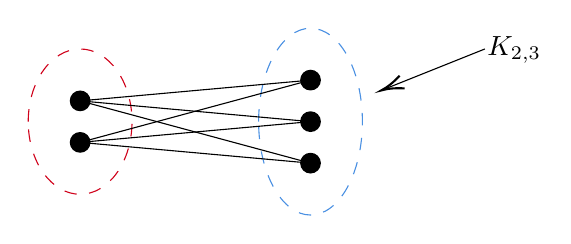
\begin{tikzpicture}[x=0.75pt,y=0.75pt,yscale=-1,xscale=1]
%uncomment if require: \path (0,273); %set diagram left start at 0, and has height of 273

%Shape: Circle [id:dp688131576532886] 
\draw  [draw opacity=0][fill={rgb, 255:red, 0; green, 0; blue, 0 }  ,fill opacity=1 ] (320,105) .. controls (320,102.24) and (322.24,100) .. (325,100) .. controls (327.76,100) and (330,102.24) .. (330,105) .. controls (330,107.76) and (327.76,110) .. (325,110) .. controls (322.24,110) and (320,107.76) .. (320,105) -- cycle ;
%Shape: Circle [id:dp06906550026981384] 
\draw  [draw opacity=0][fill={rgb, 255:red, 0; green, 0; blue, 0 }  ,fill opacity=1 ] (320,85) .. controls (320,82.24) and (322.24,80) .. (325,80) .. controls (327.76,80) and (330,82.24) .. (330,85) .. controls (330,87.76) and (327.76,90) .. (325,90) .. controls (322.24,90) and (320,87.76) .. (320,85) -- cycle ;
%Shape: Ellipse [id:dp19693373027703043] 
\draw  [color={rgb, 255:red, 208; green, 2; blue, 27 }  ,draw opacity=1 ][dash pattern={on 4.5pt off 4.5pt}] (300,95) .. controls (300,75.67) and (311.19,60) .. (325,60) .. controls (338.81,60) and (350,75.67) .. (350,95) .. controls (350,114.33) and (338.81,130) .. (325,130) .. controls (311.19,130) and (300,114.33) .. (300,95) -- cycle ;
%Shape: Circle [id:dp4998766958168427] 
\draw  [draw opacity=0][fill={rgb, 255:red, 0; green, 0; blue, 0 }  ,fill opacity=1 ] (431,115) .. controls (431,112.24) and (433.24,110) .. (436,110) .. controls (438.76,110) and (441,112.24) .. (441,115) .. controls (441,117.76) and (438.76,120) .. (436,120) .. controls (433.24,120) and (431,117.76) .. (431,115) -- cycle ;
%Shape: Circle [id:dp22040496445596047] 
\draw  [draw opacity=0][fill={rgb, 255:red, 0; green, 0; blue, 0 }  ,fill opacity=1 ] (431,95) .. controls (431,92.24) and (433.24,90) .. (436,90) .. controls (438.76,90) and (441,92.24) .. (441,95) .. controls (441,97.76) and (438.76,100) .. (436,100) .. controls (433.24,100) and (431,97.76) .. (431,95) -- cycle ;
%Shape: Circle [id:dp9638088146291519] 
\draw  [draw opacity=0][fill={rgb, 255:red, 0; green, 0; blue, 0 }  ,fill opacity=1 ] (431,75) .. controls (431,72.24) and (433.24,70) .. (436,70) .. controls (438.76,70) and (441,72.24) .. (441,75) .. controls (441,77.76) and (438.76,80) .. (436,80) .. controls (433.24,80) and (431,77.76) .. (431,75) -- cycle ;
%Shape: Ellipse [id:dp03909542165374613] 
\draw  [color={rgb, 255:red, 74; green, 144; blue, 226 }  ,draw opacity=1 ][dash pattern={on 4.5pt off 4.5pt}] (411,95) .. controls (411,70.15) and (422.19,50) .. (436,50) .. controls (449.81,50) and (461,70.15) .. (461,95) .. controls (461,119.85) and (449.81,140) .. (436,140) .. controls (422.19,140) and (411,119.85) .. (411,95) -- cycle ;
%Straight Lines [id:da14384776989856773] 
\draw [color={rgb, 255:red, 0; green, 0; blue, 0 }  ,draw opacity=1 ]   (325,85) -- (436,75) ;
%Straight Lines [id:da3420652496365374] 
\draw [color={rgb, 255:red, 0; green, 0; blue, 0 }  ,draw opacity=1 ]   (325,85) -- (436,95) ;
%Straight Lines [id:da8722228739590888] 
\draw [color={rgb, 255:red, 0; green, 0; blue, 0 }  ,draw opacity=1 ]   (325,105) -- (436,75) ;
%Straight Lines [id:da8456375684535302] 
\draw [color={rgb, 255:red, 0; green, 0; blue, 0 }  ,draw opacity=1 ]   (325,85) -- (436,115) ;
%Straight Lines [id:da21984814616627224] 
\draw [color={rgb, 255:red, 0; green, 0; blue, 0 }  ,draw opacity=1 ]   (325,105) -- (436,95) ;
%Straight Lines [id:da8265585256268246] 
\draw [color={rgb, 255:red, 0; green, 0; blue, 0 }  ,draw opacity=1 ]   (325,105) -- (436,115) ;
%Straight Lines [id:da3870623371097305] 
\draw    (520,60) -- (471.86,79.26) ;
\draw [shift={(470,80)}, rotate = 338.2] [color={rgb, 255:red, 0; green, 0; blue, 0 }  ][line width=0.75]    (10.93,-3.29) .. controls (6.95,-1.4) and (3.31,-0.3) .. (0,0) .. controls (3.31,0.3) and (6.95,1.4) .. (10.93,3.29)   ;

% Text Node
\draw (520,60.5) node [anchor=west] [inner sep=0.75pt]   [align=left] {$\displaystyle K_{2,3}$};


\end{tikzpicture}

\end{center}

If you play around a bit, you can see that $K_{3, 2}$ is planar, but we get a problem if we try use $K_{3, 3}$.

\begin{example}[$K_{3, 3}$ is Non-Planar]
	We will show that $K_{3, 3}$ is not planar.
	Note that there is 9 edges, and 6 vertices. Then by the result in the previous section, we would need $9 \leq 3 \cdot 6 - 6$, which holds. 
	
	However, recall in the proof that of our result that we had each face having at least three edges on its boundary. But that for bipartite graphs, we can get something stronger, as each face has at least four edges on its boundary (since there is no cycles of length $3$).

	So if we repeat the proof of the previous theorem with the stronger bound, we obtain $E \leq 2V - 4$, which does not hold for this graph. Thus $K_{3, 3}$ is not planar.
\end{example}

Now these two examples were interesting, but of course we care about whether \emph{any} graph is planar.  It turns out though that these are (in some sense) the \emph{only} fundamentally non-planar graphs, in that any non planar graph will have one of these graphs `behind it'.

To look at this formally, we need to look at the idea of a subdivision.

\begin{definition}[Subdivision]
	A \vocab{subdivision} of a graph $G$ is a graph $\tilde{G}$, obtained by replacing the edges of $G$ with disjoint paths.
\end{definition}

\begin{lemma}
	If $G$ is non-planar, then a subdivision of $G$ is non-planar also.
\end{lemma}
\begin{proof}
	Given a plane drawing of the subdivided graph, then by disregarding the vertices on the subdivided paths, we obtain a plane drawing of $G$ (which is a contradiction).
\end{proof}

\begin{corollary}\label{cor:planar}
	Subdivisions of $K_{3, 3}$ and $K_5$ are non-planar.
\end{corollary}
\begin{proof}
	Follows directly from the previous lemma.
\end{proof}

What ties all of this together is Kuratowski's theorem, which gives us a nice necessary and sufficient condition for a graph to be planar.

\begin{theorem}[Kuratowski's Theorem]
	A graph $G$ is planar if and only if $G$ contains no subdivisions of $K_{3, 3}$ or $K_5$.
\end{theorem}
\begin{proof}
	Omitted.\let\qed\relax
\end{proof}

We will leave the topic of planar graphs here (for now), but we note that there are some other interesting notions that are related to planarity. For example, for what graphs is it possible to draw on a torus with no edge crossings?

\section{Graph Colouring}

Informally, a graph colouring is just a way of colouring in different vertices of a graph, so that adjacent vertices are different colours. An example of a graph colouring is shown below.

\begin{center}
\tikzset{every picture/.style={line width=0.75pt}} %set default line width to 0.75pt        

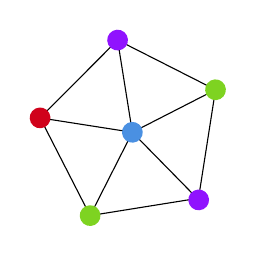
\begin{tikzpicture}[x=0.75pt,y=0.75pt,yscale=-1,xscale=1]
%uncomment if require: \path (0,293); %set diagram left start at 0, and has height of 293

%Straight Lines [id:da340779151929835] 
\draw    (309.46,139.43) -- (302.34,95) ;
%Straight Lines [id:da7087820987883349] 
\draw    (309.46,139.43) -- (349.52,118.93) ;
%Straight Lines [id:da15086021667728977] 
\draw    (309.46,139.43) -- (341.41,172) ;
%Straight Lines [id:da49162462445951893] 
\draw    (309.46,139.43) -- (289.11,179.57) ;
%Straight Lines [id:da3641220679388629] 
\draw    (309.46,139.43) -- (265,132.48) ;
%Shape: Regular Polygon [id:dp1290946675265915] 
\draw   (349.52,118.93) -- (341.34,171.19) -- (289.11,179.57) -- (265,132.48) -- (302.34,95) -- cycle ;
%Shape: Circle [id:dp3210306906760625] 
\draw  [draw opacity=0][fill={rgb, 255:red, 208; green, 2; blue, 27 }  ,fill opacity=1 ] (260.55,134.76) .. controls (259.29,132.3) and (260.26,129.29) .. (262.72,128.03) .. controls (265.18,126.77) and (268.19,127.74) .. (269.45,130.2) .. controls (270.71,132.66) and (269.74,135.67) .. (267.28,136.93) .. controls (264.82,138.19) and (261.81,137.22) .. (260.55,134.76) -- cycle ;
%Shape: Circle [id:dp8913224726118497] 
\draw  [draw opacity=0][fill={rgb, 255:red, 144; green, 19; blue, 254 }  ,fill opacity=1 ] (297.88,97.28) .. controls (296.63,94.82) and (297.6,91.81) .. (300.06,90.55) .. controls (302.52,89.29) and (305.53,90.26) .. (306.79,92.72) .. controls (308.04,95.18) and (307.07,98.19) .. (304.61,99.45) .. controls (302.16,100.71) and (299.14,99.74) .. (297.88,97.28) -- cycle ;
%Shape: Circle [id:dp2021865328138549] 
\draw  [draw opacity=0][fill={rgb, 255:red, 126; green, 211; blue, 33 }  ,fill opacity=1 ] (284.66,181.85) .. controls (283.4,179.39) and (284.37,176.38) .. (286.83,175.12) .. controls (289.29,173.86) and (292.3,174.83) .. (293.56,177.29) .. controls (294.82,179.75) and (293.84,182.76) .. (291.39,184.02) .. controls (288.93,185.28) and (285.92,184.3) .. (284.66,181.85) -- cycle ;
%Shape: Circle [id:dp39998934590743196] 
\draw  [draw opacity=0][fill={rgb, 255:red, 144; green, 19; blue, 254 }  ,fill opacity=1 ] (336.96,174.28) .. controls (335.7,171.82) and (336.67,168.81) .. (339.13,167.55) .. controls (341.59,166.29) and (344.6,167.27) .. (345.86,169.73) .. controls (347.12,172.18) and (346.14,175.2) .. (343.69,176.45) .. controls (341.23,177.71) and (338.21,176.74) .. (336.96,174.28) -- cycle ;
%Shape: Circle [id:dp02021802738298084] 
\draw  [draw opacity=0][fill={rgb, 255:red, 126; green, 211; blue, 33 }  ,fill opacity=1 ] (345.07,121.21) .. controls (343.81,118.75) and (344.78,115.73) .. (347.24,114.48) .. controls (349.7,113.22) and (352.71,114.19) .. (353.97,116.65) .. controls (355.23,119.11) and (354.25,122.12) .. (351.79,123.38) .. controls (349.34,124.64) and (346.32,123.66) .. (345.07,121.21) -- cycle ;
%Shape: Circle [id:dp2917446485192653] 
\draw  [draw opacity=0][fill={rgb, 255:red, 74; green, 144; blue, 226 }  ,fill opacity=1 ] (305.01,141.71) .. controls (303.75,139.25) and (304.72,136.24) .. (307.18,134.98) .. controls (309.64,133.72) and (312.65,134.7) .. (313.91,137.15) .. controls (315.17,139.61) and (314.2,142.63) .. (311.74,143.88) .. controls (309.28,145.14) and (306.27,144.17) .. (305.01,141.71) -- cycle ;




\end{tikzpicture}

\end{center}

\subsection{Basic Concepts}

Of course, we need to define what this means in a slightly more mathematical sense, so we will define a colouring as follows.

\begin{notation}
	We will write $[n] = \{1, 2, \dots, n\}$.
\end{notation}

\begin{definition}[$r$-Colouring]
	Let $G = (V, E)$ be a graph. An \vocab{$r$-colouring} of $G$ is a function $c : V \rightarrow [r]$ that satisfies $xy \in E \implies c(x) \neq c(y)$.
\end{definition}

An $r$-colouring divides up a graph into $r$ different \vocab{colour classes}, where there is only edges between the different colour classes.

\begin{definition}[Chromatic Number]
	The \vocab{chromatic number} of a graph $G$, denoted $\chi(G)$ is the smallest $r$ for which there exists an $r$-colouring.
\end{definition}

\begin{example}[Examples of Chromatic Numbers]
	In the graph $P_n$, we have $\chi(P_n) = 2$ for $n \geq 2$, and $\chi(P_1) = 1$.
	\begin{center}
		

\tikzset{every picture/.style={line width=0.75pt}} %set default line width to 0.75pt        

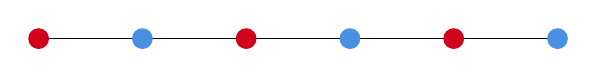
\begin{tikzpicture}[x=0.75pt,y=0.75pt,yscale=-1,xscale=1]
%uncomment if require: \path (0,93); %set diagram left start at 0, and has height of 93

%Straight Lines [id:da13160498541453314] 
\draw    (175,35) -- (425,35) ;
%Shape: Circle [id:dp5096654914635682] 
\draw  [draw opacity=0][fill={rgb, 255:red, 74; green, 144; blue, 226 }  ,fill opacity=1 ] (220,35) .. controls (220,32.24) and (222.24,30) .. (225,30) .. controls (227.76,30) and (230,32.24) .. (230,35) .. controls (230,37.76) and (227.76,40) .. (225,40) .. controls (222.24,40) and (220,37.76) .. (220,35) -- cycle ;
%Shape: Circle [id:dp757701972600446] 
\draw  [draw opacity=0][fill={rgb, 255:red, 208; green, 2; blue, 27 }  ,fill opacity=1 ] (270,35) .. controls (270,32.24) and (272.24,30) .. (275,30) .. controls (277.76,30) and (280,32.24) .. (280,35) .. controls (280,37.76) and (277.76,40) .. (275,40) .. controls (272.24,40) and (270,37.76) .. (270,35) -- cycle ;
%Shape: Circle [id:dp2235395506751915] 
\draw  [draw opacity=0][fill={rgb, 255:red, 74; green, 144; blue, 226 }  ,fill opacity=1 ] (320,35) .. controls (320,32.24) and (322.24,30) .. (325,30) .. controls (327.76,30) and (330,32.24) .. (330,35) .. controls (330,37.76) and (327.76,40) .. (325,40) .. controls (322.24,40) and (320,37.76) .. (320,35) -- cycle ;
%Shape: Circle [id:dp16894487686105397] 
\draw  [draw opacity=0][fill={rgb, 255:red, 208; green, 2; blue, 27 }  ,fill opacity=1 ] (370,35) .. controls (370,32.24) and (372.24,30) .. (375,30) .. controls (377.76,30) and (380,32.24) .. (380,35) .. controls (380,37.76) and (377.76,40) .. (375,40) .. controls (372.24,40) and (370,37.76) .. (370,35) -- cycle ;
%Shape: Circle [id:dp9181921137760612] 
\draw  [draw opacity=0][fill={rgb, 255:red, 74; green, 144; blue, 226 }  ,fill opacity=1 ] (420,35) .. controls (420,32.24) and (422.24,30) .. (425,30) .. controls (427.76,30) and (430,32.24) .. (430,35) .. controls (430,37.76) and (427.76,40) .. (425,40) .. controls (422.24,40) and (420,37.76) .. (420,35) -- cycle ;
%Shape: Circle [id:dp07969547178030623] 
\draw  [draw opacity=0][fill={rgb, 255:red, 208; green, 2; blue, 27 }  ,fill opacity=1 ] (170,35) .. controls (170,32.24) and (172.24,30) .. (175,30) .. controls (177.76,30) and (180,32.24) .. (180,35) .. controls (180,37.76) and (177.76,40) .. (175,40) .. controls (172.24,40) and (170,37.76) .. (170,35) -- cycle ;




\end{tikzpicture}

\end{center}
The graph $C_n$ has $\chi(C_n) = 2$ if $n$ is even, and $\chi(C_n) = 3$ if $n$ is odd.
\begin{center}
	

\tikzset{every picture/.style={line width=0.75pt}} %set default line width to 0.75pt        

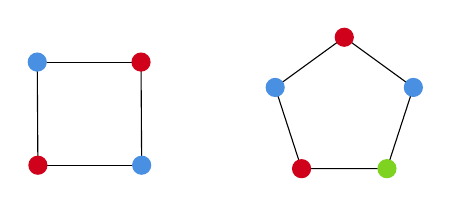
\begin{tikzpicture}[x=0.75pt,y=0.75pt,yscale=-1,xscale=1]
%uncomment if require: \path (0,175); %set diagram left start at 0, and has height of 175

%Straight Lines [id:da750036062717237] 
\draw    (209.71,56.31) -- (210.02,106) ;
%Straight Lines [id:da7912214148710233] 
\draw    (259.71,56.31) -- (260.02,106) ;
%Straight Lines [id:da6597450914019095] 
\draw    (209.71,56.31) -- (259.71,56.31) ;
%Straight Lines [id:da2008714723372247] 
\draw    (210.02,106) -- (260.02,106) ;
%Shape: Ellipse [id:dp505012491727213] 
\draw  [color={rgb, 255:red, 74; green, 144; blue, 226 }  ,draw opacity=1 ][fill={rgb, 255:red, 74; green, 144; blue, 226 }  ,fill opacity=1 ] (205.37,56.31) .. controls (205.37,53.91) and (207.31,51.96) .. (209.71,51.96) .. controls (212.11,51.96) and (214.06,53.91) .. (214.06,56.31) .. controls (214.06,58.71) and (212.11,60.65) .. (209.71,60.65) .. controls (207.31,60.65) and (205.37,58.71) .. (205.37,56.31) -- cycle ;
%Shape: Ellipse [id:dp8150490156968159] 
\draw  [color={rgb, 255:red, 208; green, 2; blue, 27 }  ,draw opacity=1 ][fill={rgb, 255:red, 208; green, 2; blue, 27 }  ,fill opacity=1 ] (255.37,56.31) .. controls (255.37,53.91) and (257.31,51.96) .. (259.71,51.96) .. controls (262.11,51.96) and (264.06,53.91) .. (264.06,56.31) .. controls (264.06,58.71) and (262.11,60.65) .. (259.71,60.65) .. controls (257.31,60.65) and (255.37,58.71) .. (255.37,56.31) -- cycle ;
%Shape: Ellipse [id:dp5133745489704719] 
\draw  [color={rgb, 255:red, 208; green, 2; blue, 27 }  ,draw opacity=1 ][fill={rgb, 255:red, 208; green, 2; blue, 27 }  ,fill opacity=1 ] (205.68,106) .. controls (205.68,103.6) and (207.62,101.65) .. (210.02,101.65) .. controls (212.42,101.65) and (214.37,103.6) .. (214.37,106) .. controls (214.37,108.4) and (212.42,110.35) .. (210.02,110.35) .. controls (207.62,110.35) and (205.68,108.4) .. (205.68,106) -- cycle ;
%Shape: Ellipse [id:dp37875023903932026] 
\draw  [color={rgb, 255:red, 74; green, 144; blue, 226 }  ,draw opacity=1 ][fill={rgb, 255:red, 74; green, 144; blue, 226 }  ,fill opacity=1 ] (255.68,106) .. controls (255.68,103.6) and (257.62,101.65) .. (260.02,101.65) .. controls (262.42,101.65) and (264.37,103.6) .. (264.37,106) .. controls (264.37,108.4) and (262.42,110.35) .. (260.02,110.35) .. controls (257.62,110.35) and (255.68,108.4) .. (255.68,106) -- cycle ;
%Shape: Regular Polygon [id:dp8600510268714245] 
\draw   (357.63,44.35) -- (390.92,68.53) -- (378.2,107.66) -- (337.06,107.66) -- (324.35,68.53) -- cycle ;
%Shape: Ellipse [id:dp34833877585191053] 
\draw  [color={rgb, 255:red, 208; green, 2; blue, 27 }  ,draw opacity=1 ][fill={rgb, 255:red, 208; green, 2; blue, 27 }  ,fill opacity=1 ] (353.29,44.35) .. controls (353.29,41.95) and (355.23,40) .. (357.63,40) .. controls (360.03,40) and (361.98,41.95) .. (361.98,44.35) .. controls (361.98,46.74) and (360.03,48.69) .. (357.63,48.69) .. controls (355.23,48.69) and (353.29,46.74) .. (353.29,44.35) -- cycle ;
%Shape: Ellipse [id:dp998768238417864] 
\draw  [color={rgb, 255:red, 74; green, 144; blue, 226 }  ,draw opacity=1 ][fill={rgb, 255:red, 74; green, 144; blue, 226 }  ,fill opacity=1 ] (320,68.53) .. controls (320,66.13) and (321.95,64.18) .. (324.35,64.18) .. controls (326.74,64.18) and (328.69,66.13) .. (328.69,68.53) .. controls (328.69,70.93) and (326.74,72.87) .. (324.35,72.87) .. controls (321.95,72.87) and (320,70.93) .. (320,68.53) -- cycle ;
%Shape: Ellipse [id:dp10085343042328077] 
\draw  [color={rgb, 255:red, 208; green, 2; blue, 27 }  ,draw opacity=1 ][fill={rgb, 255:red, 208; green, 2; blue, 27 }  ,fill opacity=1 ] (332.71,107.66) .. controls (332.71,105.26) and (334.66,103.32) .. (337.06,103.32) .. controls (339.46,103.32) and (341.4,105.26) .. (341.4,107.66) .. controls (341.4,110.06) and (339.46,112.01) .. (337.06,112.01) .. controls (334.66,112.01) and (332.71,110.06) .. (332.71,107.66) -- cycle ;
%Shape: Ellipse [id:dp1531460889801033] 
\draw  [color={rgb, 255:red, 126; green, 211; blue, 33 }  ,draw opacity=1 ][fill={rgb, 255:red, 126; green, 211; blue, 33 }  ,fill opacity=1 ] (373.86,107.66) .. controls (373.86,105.26) and (375.8,103.32) .. (378.2,103.32) .. controls (380.6,103.32) and (382.55,105.26) .. (382.55,107.66) .. controls (382.55,110.06) and (380.6,112.01) .. (378.2,112.01) .. controls (375.8,112.01) and (373.86,110.06) .. (373.86,107.66) -- cycle ;
%Shape: Ellipse [id:dp6516367663297024] 
\draw  [color={rgb, 255:red, 74; green, 144; blue, 226 }  ,draw opacity=1 ][fill={rgb, 255:red, 74; green, 144; blue, 226 }  ,fill opacity=1 ] (386.57,68.53) .. controls (386.57,66.13) and (388.52,64.18) .. (390.92,64.18) .. controls (393.32,64.18) and (395.26,66.13) .. (395.26,68.53) .. controls (395.26,70.93) and (393.32,72.87) .. (390.92,72.87) .. controls (388.52,72.87) and (386.57,70.93) .. (386.57,68.53) -- cycle ;




\end{tikzpicture}

\end{center}

The complete graph $K_n$ has $\chi(K_n) = n$.
\begin{center}
	

\tikzset{every picture/.style={line width=0.75pt}} %set default line width to 0.75pt        

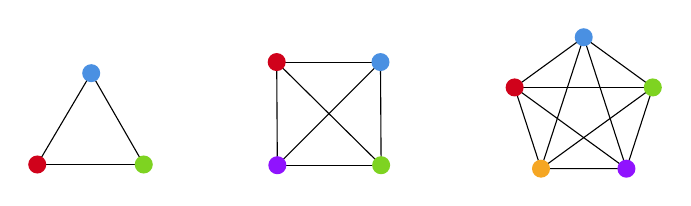
\begin{tikzpicture}[x=0.75pt,y=0.75pt,yscale=-1,xscale=1]
%uncomment if require: \path (0,175); %set diagram left start at 0, and has height of 175

%Straight Lines [id:da5950134115007302] 
\draw    (259.71,56.31) -- (210.02,106) ;
%Straight Lines [id:da9172456375368551] 
\draw    (209.71,56.31) -- (260.02,106) ;
%Straight Lines [id:da6014782727858075] 
\draw    (209.71,56.31) -- (210.02,106) ;
%Straight Lines [id:da26789829831867673] 
\draw    (259.71,56.31) -- (260.02,106) ;
%Straight Lines [id:da34407154003679685] 
\draw    (209.71,56.31) -- (259.71,56.31) ;
%Straight Lines [id:da6502598106578577] 
\draw    (210.02,106) -- (260.02,106) ;
%Straight Lines [id:da6093876792022511] 
\draw    (120.35,61.65) -- (94.35,105.65) ;
%Straight Lines [id:da6183562773187488] 
\draw    (120.35,61.65) -- (145.65,105.65) ;
%Straight Lines [id:da7438336681560819] 
\draw    (94.35,105.65) -- (145.65,105.65) ;
%Shape: Ellipse [id:dp910757651091173] 
\draw  [draw opacity=0][fill={rgb, 255:red, 208; green, 2; blue, 27 }  ,fill opacity=1 ] (90,105.65) .. controls (90,103.26) and (91.95,101.31) .. (94.35,101.31) .. controls (96.74,101.31) and (98.69,103.26) .. (98.69,105.65) .. controls (98.69,108.05) and (96.74,110) .. (94.35,110) .. controls (91.95,110) and (90,108.05) .. (90,105.65) -- cycle ;
%Shape: Ellipse [id:dp3476441523478542] 
\draw  [draw opacity=0][fill={rgb, 255:red, 126; green, 211; blue, 33 }  ,fill opacity=1 ] (141.31,105.65) .. controls (141.31,103.26) and (143.26,101.31) .. (145.65,101.31) .. controls (148.05,101.31) and (150,103.26) .. (150,105.65) .. controls (150,108.05) and (148.05,110) .. (145.65,110) .. controls (143.26,110) and (141.31,108.05) .. (141.31,105.65) -- cycle ;
%Shape: Ellipse [id:dp8017310543412064] 
\draw  [draw opacity=0][fill={rgb, 255:red, 74; green, 144; blue, 226 }  ,fill opacity=1 ] (116,61.65) .. controls (116,59.26) and (117.95,57.31) .. (120.35,57.31) .. controls (122.74,57.31) and (124.69,59.26) .. (124.69,61.65) .. controls (124.69,64.05) and (122.74,66) .. (120.35,66) .. controls (117.95,66) and (116,64.05) .. (116,61.65) -- cycle ;
%Shape: Ellipse [id:dp4259339991452087] 
\draw  [draw opacity=0][fill={rgb, 255:red, 208; green, 2; blue, 27 }  ,fill opacity=1 ] (205.37,56.31) .. controls (205.37,53.91) and (207.31,51.96) .. (209.71,51.96) .. controls (212.11,51.96) and (214.06,53.91) .. (214.06,56.31) .. controls (214.06,58.71) and (212.11,60.65) .. (209.71,60.65) .. controls (207.31,60.65) and (205.37,58.71) .. (205.37,56.31) -- cycle ;
%Shape: Ellipse [id:dp3272067927292138] 
\draw  [draw opacity=0][fill={rgb, 255:red, 74; green, 144; blue, 226 }  ,fill opacity=1 ] (255.37,56.31) .. controls (255.37,53.91) and (257.31,51.96) .. (259.71,51.96) .. controls (262.11,51.96) and (264.06,53.91) .. (264.06,56.31) .. controls (264.06,58.71) and (262.11,60.65) .. (259.71,60.65) .. controls (257.31,60.65) and (255.37,58.71) .. (255.37,56.31) -- cycle ;
%Shape: Ellipse [id:dp6279471584081898] 
\draw  [draw opacity=0][fill={rgb, 255:red, 144; green, 19; blue, 254 }  ,fill opacity=1 ] (205.68,106) .. controls (205.68,103.6) and (207.62,101.65) .. (210.02,101.65) .. controls (212.42,101.65) and (214.37,103.6) .. (214.37,106) .. controls (214.37,108.4) and (212.42,110.35) .. (210.02,110.35) .. controls (207.62,110.35) and (205.68,108.4) .. (205.68,106) -- cycle ;
%Shape: Ellipse [id:dp2716753232633131] 
\draw  [draw opacity=0][fill={rgb, 255:red, 126; green, 211; blue, 33 }  ,fill opacity=1 ] (255.68,106) .. controls (255.68,103.6) and (257.62,101.65) .. (260.02,101.65) .. controls (262.42,101.65) and (264.37,103.6) .. (264.37,106) .. controls (264.37,108.4) and (262.42,110.35) .. (260.02,110.35) .. controls (257.62,110.35) and (255.68,108.4) .. (255.68,106) -- cycle ;
%Shape: Regular Polygon [id:dp3759703669416229] 
\draw   (357.63,44.35) -- (390.92,68.53) -- (378.2,107.66) -- (337.06,107.66) -- (324.35,68.53) -- cycle ;
%Straight Lines [id:da13577702647900103] 
\draw    (324.35,68.53) -- (378.2,107.66) ;
%Straight Lines [id:da9997872113436649] 
\draw    (337.06,107.66) -- (390.92,68.53) ;
%Straight Lines [id:da9115474312921606] 
\draw    (337.06,107.66) -- (357.63,44.35) ;
%Straight Lines [id:da8883836326932297] 
\draw    (324.35,68.53) -- (390.92,68.53) ;
%Straight Lines [id:da7855939638113758] 
\draw    (357.63,44.35) -- (378.2,107.66) ;
%Shape: Ellipse [id:dp8834156534578096] 
\draw  [draw opacity=0][fill={rgb, 255:red, 74; green, 144; blue, 226 }  ,fill opacity=1 ] (353.29,44.35) .. controls (353.29,41.95) and (355.23,40) .. (357.63,40) .. controls (360.03,40) and (361.98,41.95) .. (361.98,44.35) .. controls (361.98,46.74) and (360.03,48.69) .. (357.63,48.69) .. controls (355.23,48.69) and (353.29,46.74) .. (353.29,44.35) -- cycle ;
%Shape: Ellipse [id:dp9133677918155244] 
\draw  [draw opacity=0][fill={rgb, 255:red, 208; green, 2; blue, 27 }  ,fill opacity=1 ] (320,68.53) .. controls (320,66.13) and (321.95,64.18) .. (324.35,64.18) .. controls (326.74,64.18) and (328.69,66.13) .. (328.69,68.53) .. controls (328.69,70.93) and (326.74,72.87) .. (324.35,72.87) .. controls (321.95,72.87) and (320,70.93) .. (320,68.53) -- cycle ;
%Shape: Ellipse [id:dp41555024135442464] 
\draw  [draw opacity=0][fill={rgb, 255:red, 245; green, 166; blue, 35 }  ,fill opacity=1 ] (332.71,107.66) .. controls (332.71,105.26) and (334.66,103.32) .. (337.06,103.32) .. controls (339.46,103.32) and (341.4,105.26) .. (341.4,107.66) .. controls (341.4,110.06) and (339.46,112.01) .. (337.06,112.01) .. controls (334.66,112.01) and (332.71,110.06) .. (332.71,107.66) -- cycle ;
%Shape: Ellipse [id:dp6758412806241771] 
\draw  [draw opacity=0][fill={rgb, 255:red, 144; green, 19; blue, 254 }  ,fill opacity=1 ] (373.86,107.66) .. controls (373.86,105.26) and (375.8,103.32) .. (378.2,103.32) .. controls (380.6,103.32) and (382.55,105.26) .. (382.55,107.66) .. controls (382.55,110.06) and (380.6,112.01) .. (378.2,112.01) .. controls (375.8,112.01) and (373.86,110.06) .. (373.86,107.66) -- cycle ;
%Shape: Ellipse [id:dp18313604355533142] 
\draw  [draw opacity=0][fill={rgb, 255:red, 126; green, 211; blue, 33 }  ,fill opacity=1 ] (386.57,68.53) .. controls (386.57,66.13) and (388.52,64.18) .. (390.92,64.18) .. controls (393.32,64.18) and (395.26,66.13) .. (395.26,68.53) .. controls (395.26,70.93) and (393.32,72.87) .. (390.92,72.87) .. controls (388.52,72.87) and (386.57,70.93) .. (386.57,68.53) -- cycle ;




\end{tikzpicture}
\end{center}
\end{example}

The case for $C_{2n}$ follows from a more general fact about bipartite graphs.

\begin{proposition}[Chromatic Number of Bipartite Graphs]
	If $G$ is a bipartite graph, then $\chi(G) \leq 2$, and indeed $\chi(G) = 2$ unless $E = \emptyset$.
\end{proposition}
\begin{proof}[Proof Sketch] Colour the vertices in each part separately.
\end{proof}

Indeed, one way to think about chromatic number is as a generalization of bipartite graphs to multiple parts.

A straightforward observation to make is that the maximum degree of a graph ($\Delta$) puts a bound on the chromatic number.

\begin{proposition}[Degree Bound for Chromatic Number]\label{prop:degbound}
	For a graph $G$, we have $\chi(G) \leq \Delta(G) + 1$. This bound is also sharp\footnote{Take the complete graph or odd cycles. These are the only such examples though}.
\end{proposition}

To prove this, we are going to use a type of greedy algorithm.

\begin{definition}[Greedy Colouring]
	Given a graph $G = (V, E)$ with vertices $V = \{v_1, v_2, \dots, v_n\}$, the \vocab{greedy colouring} of $G$ is a function $c_g: V\rightarrow \N$ defined inductively by
	\begin{itemize}
		\item $c_g(v_1) = 1$,
		\item Given coloured $v_1, \dots, v_t$, we have $c_g(v_{t + 1}) = \min(\N\backslash \{c(v_i) \mid v_i \sim v_{t + 1}, i \leq t\})$.
	\end{itemize}
\end{definition}

\begin{proof}[Proof of \autoref{prop:degbound}]
	Apply the greedy colouring to $G$ with an arbitrary vertex ordering $v_1, \dots, v_n$. Then we note that
	$$
	|\{c(v_i) \mid v_i \sim v_{t + 1}, i \leq t\}| \leq \Delta(G),
	$$
	and thus $c_g(v_{t + 1}) \in [\Delta + 1]$.
\end{proof}

The `greedy' approach need not give you any colouring that's in any way optimal. For example, if we have the graph $P_4$ with vertices labelled as below, we get the following colouring from our greedy approach.

\begin{center}
	

\tikzset{every picture/.style={line width=0.75pt}} %set default line width to 0.75pt        

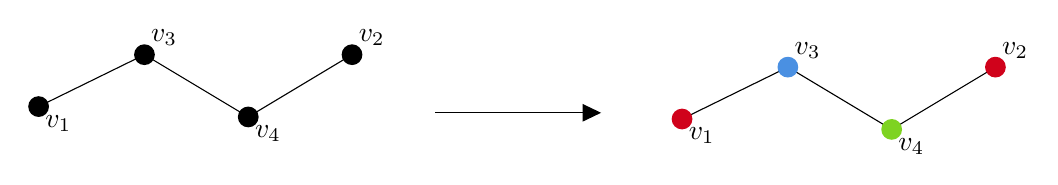
\begin{tikzpicture}[x=0.75pt,y=0.75pt,yscale=-1,xscale=1]
%uncomment if require: \path (0,273); %set diagram left start at 0, and has height of 273

%Straight Lines [id:da2632641420696793] 
\draw    (69,127) -- (120,102) ;
%Straight Lines [id:da08919587757626957] 
\draw [color={rgb, 255:red, 0; green, 0; blue, 0 }  ,draw opacity=1 ]   (120,102) -- (170,132) ;
%Straight Lines [id:da015358028892263231] 
\draw    (170,132) -- (220,102) ;
%Shape: Circle [id:dp676123344285424] 
\draw  [draw opacity=0][fill={rgb, 255:red, 0; green, 0; blue, 0 }  ,fill opacity=1 ] (64,127) .. controls (64,124.24) and (66.24,122) .. (69,122) .. controls (71.76,122) and (74,124.24) .. (74,127) .. controls (74,129.76) and (71.76,132) .. (69,132) .. controls (66.24,132) and (64,129.76) .. (64,127) -- cycle ;
%Shape: Circle [id:dp6368387482394398] 
\draw  [draw opacity=0][fill={rgb, 255:red, 0; green, 0; blue, 0 }  ,fill opacity=1 ] (115,102) .. controls (115,99.24) and (117.24,97) .. (120,97) .. controls (122.76,97) and (125,99.24) .. (125,102) .. controls (125,104.76) and (122.76,107) .. (120,107) .. controls (117.24,107) and (115,104.76) .. (115,102) -- cycle ;
%Shape: Circle [id:dp6381785951038155] 
\draw  [draw opacity=0][fill={rgb, 255:red, 0; green, 0; blue, 0 }  ,fill opacity=1 ] (165,132) .. controls (165,129.24) and (167.24,127) .. (170,127) .. controls (172.76,127) and (175,129.24) .. (175,132) .. controls (175,134.76) and (172.76,137) .. (170,137) .. controls (167.24,137) and (165,134.76) .. (165,132) -- cycle ;
%Shape: Circle [id:dp8419003008424625] 
\draw  [draw opacity=0][fill={rgb, 255:red, 0; green, 0; blue, 0 }  ,fill opacity=1 ] (215,102) .. controls (215,99.24) and (217.24,97) .. (220,97) .. controls (222.76,97) and (225,99.24) .. (225,102) .. controls (225,104.76) and (222.76,107) .. (220,107) .. controls (217.24,107) and (215,104.76) .. (215,102) -- cycle ;
%Straight Lines [id:da7901383388583939] 
\draw    (260,130) -- (337,130) ;
\draw [shift={(340,130)}, rotate = 180] [fill={rgb, 255:red, 0; green, 0; blue, 0 }  ][line width=0.08]  [draw opacity=0] (8.93,-4.29) -- (0,0) -- (8.93,4.29) -- cycle    ;
%Straight Lines [id:da9429927636641652] 
\draw    (379,133) -- (430,108) ;
%Straight Lines [id:da19780480807889433] 
\draw [color={rgb, 255:red, 0; green, 0; blue, 0 }  ,draw opacity=1 ]   (430,108) -- (480,138) ;
%Straight Lines [id:da36377018396002936] 
\draw    (480,138) -- (530,108) ;
%Shape: Circle [id:dp9969326950548666] 
\draw  [draw opacity=0][fill={rgb, 255:red, 208; green, 2; blue, 27 }  ,fill opacity=1 ] (374,133) .. controls (374,130.24) and (376.24,128) .. (379,128) .. controls (381.76,128) and (384,130.24) .. (384,133) .. controls (384,135.76) and (381.76,138) .. (379,138) .. controls (376.24,138) and (374,135.76) .. (374,133) -- cycle ;
%Shape: Circle [id:dp7314073199094315] 
\draw  [draw opacity=0][fill={rgb, 255:red, 74; green, 144; blue, 226 }  ,fill opacity=1 ] (425,108) .. controls (425,105.24) and (427.24,103) .. (430,103) .. controls (432.76,103) and (435,105.24) .. (435,108) .. controls (435,110.76) and (432.76,113) .. (430,113) .. controls (427.24,113) and (425,110.76) .. (425,108) -- cycle ;
%Shape: Circle [id:dp8979235152955327] 
\draw  [draw opacity=0][fill={rgb, 255:red, 126; green, 211; blue, 33 }  ,fill opacity=1 ] (475,138) .. controls (475,135.24) and (477.24,133) .. (480,133) .. controls (482.76,133) and (485,135.24) .. (485,138) .. controls (485,140.76) and (482.76,143) .. (480,143) .. controls (477.24,143) and (475,140.76) .. (475,138) -- cycle ;
%Shape: Circle [id:dp43828607417418664] 
\draw  [draw opacity=0][fill={rgb, 255:red, 208; green, 2; blue, 27 }  ,fill opacity=1 ] (525,108) .. controls (525,105.24) and (527.24,103) .. (530,103) .. controls (532.76,103) and (535,105.24) .. (535,108) .. controls (535,110.76) and (532.76,113) .. (530,113) .. controls (527.24,113) and (525,110.76) .. (525,108) -- cycle ;

% Text Node
\draw (71,130) node [anchor=north west][inner sep=0.75pt]    {$v_{1}$};
% Text Node
\draw (122,99) node [anchor=south west] [inner sep=0.75pt]    {$v_{3}$};
% Text Node
\draw (222,99) node [anchor=south west] [inner sep=0.75pt]    {$v_{2}$};
% Text Node
\draw (172,135) node [anchor=north west][inner sep=0.75pt]    {$v_{4}$};
% Text Node
\draw (381,136) node [anchor=north west][inner sep=0.75pt]    {$v_{1}$};
% Text Node
\draw (432,105) node [anchor=south west] [inner sep=0.75pt]    {$v_{3}$};
% Text Node
\draw (532,105) node [anchor=south west] [inner sep=0.75pt]    {$v_{2}$};
% Text Node
\draw (482,141) node [anchor=north west][inner sep=0.75pt]    {$v_{4}$};


\end{tikzpicture}

\end{center}
This is clearly not optimal.

\subsection{Brooks' Theorem}

One step up from the greedy approach to obtaining a colouring comes in the form of Brooks' Theorem. Before we look at that, we will make an observation.

\begin{proposition}
	Let $G$ be a connected graph for which $\delta(G) < \Delta(G)$. Then $\chi(G) \leq \Delta(G)$.
\end{proposition}
\begin{proof}
	% Order the vertices so that every vertex (except the last) has a `backwards' edge, and then put a vertex with degree $\leq \Delta(G) - 1$ at the end.
	We find a better ordering to apply the greedy colouring to. First define $v_n = v$, where $d(v) \leq \Delta(G) - 1$. Now choose an ordering of $v_1, \dots, v_{n - 1}$ so that
	$$
	d(v_1, v) \geq d(v_2, v) \geq \cdots \geq d(v_{n - 1}, v).
	$$
	We claim that each vertex $v_i$ with $i \in [n - 1]$ has at most $\Delta(G) - 1$ neighbors in $v_1, \dots, v_{i - 1}$.

	This is true for $v_n$ by definition. For $v_i$ with $i \neq n$, we observe that a shortest path $P$ from $v_i$ to $v_n$ contains a neighbor $v_j$ of $v_i$ with $d(v_j, v) < d(v_i, v)$. Thus $v_j$ comes later in the ordering (that is, $j > i$).

	So the greedy colouring gives each vertex one of $\Delta(G)$ colours.
\end{proof}

We can now extend this idea to prove Brook's theorem.

\begin{theorem}[Brooks' Theorem]
	Let $G$ be a connected graph that is not complete or an odd cycle. Then $\chi(G) \leq \Delta(G)$.
\end{theorem}
\begin{proof}
	Let $G$ be a counterexample with a minimal number of edges.
	We may assume $G$ is a regular graph ($\Delta$-regular), and also that $\Delta \geq 3$.

	Since $G$ is not complete, there exists a vertex $v \in V(G)$ so that $G[N(V)]$ is not complete, and let $x, y \in N(v)$ where $x \sim y$ and $x \neq y$. 

	If $G$ is 3-connected then $G' = G - x - y$ is connected. In this case, we order the vertices of $G'$ by $v_1 = x$, $v_2 = y$, and $v_n = v$. Then we define $v_3, \dots, v_{n - 1}$ by ordering the vertices of $G'$ so that
	$$
		d_{G'}(v_3, v) \geq d_{G'}(v_4, v) \geq \cdots \geq d_{G'}(v_{n - 1}, v).
	$$
	
	As we saw before, the greedy colouring with the ordering $v_1, \dots, v_n$ will give us a $\Delta$-colouring of $G$.

	If $G$ has a cut vertex $w \in V$, then let $G- w = C_1 \cup \cdots \cup C_k$ be the components, and $G_i = G[C_i \cup \{w\}]$. The maximum degree in $G_i$ is bounded by $\Delta$, and therefore $G_i$ has a $\Delta$-colouring for each $i$, by the minimality of the counter example. 
	Note that $G_i$ cannot be a complete graph on $\Delta + 1$ vertices since $d_{G_i}(w) \leq \Delta - 1$.
	By permuting the colours, we can assume each colouring gives the vertex $w$ colour 1. Thus we have a colouring of $G$ with $\Delta$ colours, which is a contradiction.

	If $G-\{w_1, w_2\}$ is disconnected for $w_1 \neq w_2$ with $w_1, w_2 \in V$, then let $C_1, \dots, C_k$ be the components of $G - \{w_1, w_2\}$. We may assume that $G$ has no cut vertex by the previous case. Now let $G_i = G[C_i \cup \{w_1, w_2\}]+ w_1w_2$. Note that $e(G_i) < e(G)$ since $w_1, w_2$ both send at least one edge to each component $C_1, \dots, C_k$. Also $d_{G_i}(w_1) \leq \Delta$ and likewise $d_{G_i}(w_2) \leq \Delta$, thus the maximum degree $G_i \leq \Delta$ and thus we can find a $\Delta$-colouring of $G_i$ for each $i$. That gives $w_1, w_2$ different colours. After permuting these colours, I can assume $w_1$ is coloured $1$ in each, and $w_2$ is coloured 2 in each. Thus we can put all of the colourings together to obtain a colouring of $G$.
\end{proof}

\subsection{Colouring Planar Graphs}

We will now consider colourings on graphs that are planar. It is in this section that the theorem ever-present in the popular maths psyche is kept (without proof).

\begin{theorem}[Four-Colour Theorem]
	Let $G$ be a planar graph. Then $\chi(G) \leq 4$.
\end{theorem}

Or informally: any map can be coloured with only four colours, where neighboring regions have different colours. Note that this is the duel form of the theorem above.
This theorem was proved in 1976 by Appel \& Haken and centers around reducing the theorem to a large number of cases, that were checked by computer.

We are going to prove two slightly weaker versions, that are still quite interesting.

\begin{theorem}[Six Colour Theorem -- Warmup]
Let $G$ be a planar graph. Then $\chi(G) \leq G$.
\end{theorem}
\begin{proof}
	We will use induction on $n = |G|$. For $n = 1$, this is trivial.
	Now inductively, we claim that there is a vertex $v$ with $\deg(v) \leq 5$. We note
	$$
	\frac{1}{n}\left[\sum_{x \in V} d(x)\right] = \frac{2E}{n} \leq 6 - \frac{12}{n} < 6.
	$$
	Thus there is a vertex $v$ with $\deg(v) \leq 5$. By induction, $G - v$ is 6-colourable, and since $v$ has at most 5 neighbors, there is a colour in $[6]$ that does not appear in $N(v)$. Colouring $v$ with this colour, we get that the graph is 6-colourable.
\end{proof}

Now we are going to kick it up a notch shortly, by introducing one more ingredient.

\begin{definition}
	Given a graph $G$ and an $r$-colouring of $G$, let $v \in V(G)$, and define the \vocab{$\{i, j\}$-component of $v$} to be all of the vertices that can be reached starting at $v$ along a path using only colours $i$ and $j$.
\end{definition}

We make the following observation, which gives us an extra `move' to use in the stronger proof

\begin{proposition}
Given a graph $G$ with an $r$-colouring $c$, and for $i, j \in [v]$ with $i, j$, we can \emph{swap} the colour on an $\{i, j\}$-component to obtain a new colouring.	
\end{proposition}
\begin{proof}[Proof Sketch]
	This works because of the `being reached' condition in the $\{i, j\}$-component definition.
\end{proof}

Now we can prove the five colour theorem, using a lot of the ideas from the proof of the six colour theorem.

\begin{theorem}[Five Colour Theorem]
	Let $G$ be a planar graph. Then $\chi(G) \leq G$.
\end{theorem}
\begin{proof}
	By induction on $n = |G|$, we note $n = 1$ is trivial.
	Now we proceed with the induction step. Let $v$ be a vertex with $d(v) \leq 5$. Then apply induction to get a 5-colouring of $G - v$. Let $N(V) = \{x_1, \dots, x_5\}$, where $x_1, \dots, x_5$ are arranged in a clockwise manner. We may assume that $c(x_i) = i$ (otherwise we can colour $v$ with the missing colour).

	Now consider the $\{1, 3\}$-component containing $x_1$. If $x_3$ is not in this component, we can swap colours on this $\{1, 3\}$ component so that $x_1$ is colored with $3$, and then colour $v$ with 1. 

	So we may assume there exists a path $x_1 \rightarrow x_3$ using colours $1$ and $3$ only. By the same argument there exists a path $x_2 \rightarrow x_4$ using colours 2 and 4 only. But then these paths must share a vertex, which is a contradiction.
\end{proof}

\subsection{Colouring Graphs on (Other) Surfaces}

Following on from the last section, we will consider a related guiding question:
\begin{center}
	If $G$ is a graph, drawn on the torus, what can we say about $\chi(G)$?
\end{center}
More generally, if $G$ is a graph drawn on a surface of genus $g$, what can we say about $\chi(G)$? For example, the graph $K_7$ can be drawn on a torus without edge crossings.
\begin{center}
	



	\tikzset{every picture/.style={line width=0.75pt}} %set default line width to 0.75pt        

	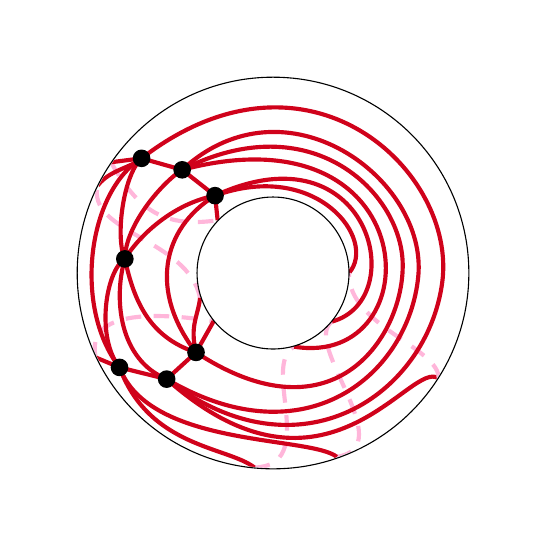
\begin{tikzpicture}[x=0.75pt,y=0.75pt,yscale=-0.85,xscale=0.85]
	%uncomment if require: \path (0,273); %set diagram left start at 0, and has height of 273
	
	%Curve Lines [id:da4978886062387847] 
	\draw [color={rgb, 255:red, 208; green, 2; blue, 27 }  ,draw opacity=1 ][line width=1.5]    (523.4,188.8) .. controls (507.8,176.8) and (460.2,270) .. (369.21,189.14) ;
	%Curve Lines [id:da2787755833466724] 
	\draw [color={rgb, 255:red, 208; green, 2; blue, 27 }  ,draw opacity=1 ][line width=1.5]    (396.64,85.14) .. controls (454.2,64.4) and (489,110) .. (472.57,129) ;
	%Curve Lines [id:da293843798760554] 
	\draw [color={rgb, 255:red, 255; green, 182; blue, 218 }  ,draw opacity=1 ][line width=1.5]  [dash pattern={on 5.63pt off 4.5pt}]  (523.4,188.8) .. controls (523.8,171.2) and (471.8,158.8) .. (472.57,129) ;
	%Curve Lines [id:da5293940677817494] 
	\draw [color={rgb, 255:red, 255; green, 182; blue, 218 }  ,draw opacity=1 ][line width=1.5]  [dash pattern={on 5.63pt off 4.5pt}]  (465.67,233.17) .. controls (502.33,227.83) and (445.33,168.5) .. (463,156.5) ;
	%Curve Lines [id:da8043955346758574] 
	\draw [color={rgb, 255:red, 255; green, 182; blue, 218 }  ,draw opacity=1 ][line width=1.5]  [dash pattern={on 5.63pt off 4.5pt}]  (419,239.25) .. controls (456.1,238.05) and (422.3,181.55) .. (441.5,170.75) ;
	%Curve Lines [id:da713618048686119] 
	\draw [color={rgb, 255:red, 255; green, 182; blue, 218 }  ,draw opacity=1 ][line width=1.5]  [dash pattern={on 5.63pt off 4.5pt}]  (337.67,66.22) .. controls (341.88,73.74) and (346.02,79.83) .. (350.33,84.66) .. controls (362.85,98.67) and (376.79,102.09) .. (398.11,99.11) ;
	%Curve Lines [id:da1240776254039353] 
	\draw [color={rgb, 255:red, 255; green, 182; blue, 218 }  ,draw opacity=1 ][line width=1.5]  [dash pattern={on 5.63pt off 4.5pt}]  (388.14,143.14) .. controls (381.57,109.71) and (323.57,106.29) .. (330.14,79.43) ;
	%Curve Lines [id:da4453074798326062] 
	\draw [color={rgb, 255:red, 255; green, 182; blue, 218 }  ,draw opacity=1 ][line width=1.5]  [dash pattern={on 5.63pt off 4.5pt}]  (329,176.86) .. controls (324.14,154.86) and (349.57,149.14) .. (395.86,156.29) ;
	
	%Curve Lines [id:da22514304721216527] 
	\draw [color={rgb, 255:red, 208; green, 2; blue, 27 }  ,draw opacity=1 ][line width=1.5]    (378,70.5) .. controls (437,16) and (517.4,76) .. (511.8,131.2) .. controls (506.2,186.4) and (448.2,235.6) .. (369.21,189.14) ;
	%Curve Lines [id:da7154042099957507] 
	\draw [color={rgb, 255:red, 208; green, 2; blue, 27 }  ,draw opacity=1 ][line width=1.5]    (378,70.5) .. controls (451,33.2) and (502.2,83.2) .. (503,123.6) .. controls (503.8,164) and (464.6,225.6) .. (385.86,174) ;
	%Curve Lines [id:da7681022452406513] 
	\draw [color={rgb, 255:red, 208; green, 2; blue, 27 }  ,draw opacity=1 ][line width=1.5]    (419,239.25) .. controls (403.4,227.25) and (359.4,228) .. (342.5,182.5) ;
	%Curve Lines [id:da5471317621058147] 
	\draw [color={rgb, 255:red, 208; green, 2; blue, 27 }  ,draw opacity=1 ][line width=1.5]    (378,70.5) .. controls (517.4,33.6) and (520.2,183.6) .. (441.5,170.75) ;
	%Curve Lines [id:da0542368094347222] 
	\draw [color={rgb, 255:red, 208; green, 2; blue, 27 }  ,draw opacity=1 ][line width=1.5]    (396.64,85.14) .. controls (484.2,44.8) and (508.2,144) .. (463,156.5) ;
	%Curve Lines [id:da4609584594796077] 
	\draw [color={rgb, 255:red, 208; green, 2; blue, 27 }  ,draw opacity=1 ][line width=1.5]    (465.67,233.17) .. controls (450.07,221.17) and (359.4,228) .. (342.5,182.5) ;
	%Straight Lines [id:da7022526259473441] 
	\draw [color={rgb, 255:red, 208; green, 2; blue, 27 }  ,draw opacity=1 ][line width=1.5]    (355,64) -- (378,70.5) ;
	%Straight Lines [id:da00320666581798823] 
	\draw [color={rgb, 255:red, 208; green, 2; blue, 27 }  ,draw opacity=1 ][line width=1.5]    (378,70.5) -- (396.64,85.14) ;
	%Straight Lines [id:da3588612751365804] 
	\draw [color={rgb, 255:red, 208; green, 2; blue, 27 }  ,draw opacity=1 ][line width=1.5]    (369.21,189.14) -- (385.86,174) ;
	%Straight Lines [id:da740956795390784] 
	\draw [color={rgb, 255:red, 208; green, 2; blue, 27 }  ,draw opacity=1 ][line width=1.5]    (342.5,182.5) -- (369.21,189.14) ;
	%Curve Lines [id:da2574195365628378] 
	\draw [color={rgb, 255:red, 208; green, 2; blue, 27 }  ,draw opacity=1 ][line width=1.5]    (345.5,121) .. controls (339.86,108.57) and (344.71,73.14) .. (355,64) ;
	%Curve Lines [id:da9661714973882507] 
	\draw [color={rgb, 255:red, 208; green, 2; blue, 27 }  ,draw opacity=1 ][line width=1.5]    (345.5,121) .. controls (354.71,106.29) and (374.14,89.43) .. (396.64,85.14) ;
	%Curve Lines [id:da49116042398727233] 
	\draw [color={rgb, 255:red, 208; green, 2; blue, 27 }  ,draw opacity=1 ][line width=1.5]    (345.5,121) .. controls (345.86,101.43) and (367,77.43) .. (378,70.5) ;
	%Curve Lines [id:da1702178597675068] 
	\draw [color={rgb, 255:red, 208; green, 2; blue, 27 }  ,draw opacity=1 ][line width=1.5]    (342.5,182.5) .. controls (329,165.71) and (334.5,127.93) .. (345.5,121) ;
	%Curve Lines [id:da7670962741541075] 
	\draw [color={rgb, 255:red, 208; green, 2; blue, 27 }  ,draw opacity=1 ][line width=1.5]    (369.21,189.14) .. controls (342.14,178) and (339,143.43) .. (345.5,121) ;
	%Curve Lines [id:da3093014186492592] 
	\draw [color={rgb, 255:red, 208; green, 2; blue, 27 }  ,draw opacity=1 ][line width=1.5]    (385.86,174) .. controls (359,165.14) and (350.71,144.57) .. (345.5,121) ;
	%Curve Lines [id:da6724433431143393] 
	\draw [color={rgb, 255:red, 208; green, 2; blue, 27 }  ,draw opacity=1 ][line width=1.5]    (385.86,174) .. controls (359.29,139.71) and (366.14,104) .. (396.64,85.14) ;
	%Curve Lines [id:da010503462076410397] 
	\draw [color={rgb, 255:red, 208; green, 2; blue, 27 }  ,draw opacity=1 ][line width=1.5]    (342.5,182.5) .. controls (315.93,148.21) and (324.5,82.86) .. (355,64) ;
	%Curve Lines [id:da5002970294046724] 
	\draw [color={rgb, 255:red, 208; green, 2; blue, 27 }  ,draw opacity=1 ][line width=1.5]    (355,64) .. controls (449.5,-8.75) and (533.9,71.4) .. (525.4,134.4) .. controls (516.9,197.4) and (445,247.75) .. (369.21,189.14) ;
	%Straight Lines [id:da9083881608203679] 
	\draw [color={rgb, 255:red, 208; green, 2; blue, 27 }  ,draw opacity=1 ][line width=1.5]    (337.67,66.22) -- (355,64) ;
	%Straight Lines [id:da26022148663016753] 
	\draw [color={rgb, 255:red, 208; green, 2; blue, 27 }  ,draw opacity=1 ][line width=1.5]    (396.64,85.14) -- (398.11,99.11) ;
	%Curve Lines [id:da36267323386140404] 
	\draw [color={rgb, 255:red, 208; green, 2; blue, 27 }  ,draw opacity=1 ][line width=1.5]    (385.86,174) .. controls (382.14,158.86) and (387,153.43) .. (388.14,143.14) ;
	%Curve Lines [id:da630318287371103] 
	\draw [color={rgb, 255:red, 208; green, 2; blue, 27 }  ,draw opacity=1 ][line width=1.5]    (330.14,79.43) .. controls (336.71,70.57) and (349.57,69.14) .. (355,64) ;
	%Straight Lines [id:da6227799714994595] 
	\draw [color={rgb, 255:red, 208; green, 2; blue, 27 }  ,draw opacity=1 ][line width=1.5]    (329,176.86) -- (342.5,182.5) ;
	%Straight Lines [id:da3712871884760477] 
	\draw [color={rgb, 255:red, 208; green, 2; blue, 27 }  ,draw opacity=1 ][line width=1.5]    (395.86,156.29) -- (385.86,174) ;
	%Shape: Circle [id:dp1570173947239496] 
	\draw  [draw opacity=0][fill={rgb, 255:red, 0; green, 0; blue, 0 }  ,fill opacity=1 ] (340.5,121) .. controls (340.5,118.24) and (342.74,116) .. (345.5,116) .. controls (348.26,116) and (350.5,118.24) .. (350.5,121) .. controls (350.5,123.76) and (348.26,126) .. (345.5,126) .. controls (342.74,126) and (340.5,123.76) .. (340.5,121) -- cycle ;
	%Shape: Circle [id:dp5724587970250766] 
	\draw  [draw opacity=0][fill={rgb, 255:red, 0; green, 0; blue, 0 }  ,fill opacity=1 ] (350,64) .. controls (350,61.24) and (352.24,59) .. (355,59) .. controls (357.76,59) and (360,61.24) .. (360,64) .. controls (360,66.76) and (357.76,69) .. (355,69) .. controls (352.24,69) and (350,66.76) .. (350,64) -- cycle ;
	%Shape: Circle [id:dp9075764504295125] 
	\draw  [draw opacity=0][fill={rgb, 255:red, 0; green, 0; blue, 0 }  ,fill opacity=1 ] (373,70.5) .. controls (373,67.74) and (375.24,65.5) .. (378,65.5) .. controls (380.76,65.5) and (383,67.74) .. (383,70.5) .. controls (383,73.26) and (380.76,75.5) .. (378,75.5) .. controls (375.24,75.5) and (373,73.26) .. (373,70.5) -- cycle ;
	%Shape: Circle [id:dp8392302198280852] 
	\draw  [draw opacity=0][fill={rgb, 255:red, 0; green, 0; blue, 0 }  ,fill opacity=1 ] (391.64,85.14) .. controls (391.64,82.38) and (393.88,80.14) .. (396.64,80.14) .. controls (399.4,80.14) and (401.64,82.38) .. (401.64,85.14) .. controls (401.64,87.9) and (399.4,90.14) .. (396.64,90.14) .. controls (393.88,90.14) and (391.64,87.9) .. (391.64,85.14) -- cycle ;
	%Shape: Circle [id:dp8144563152928861] 
	\draw  [draw opacity=0][fill={rgb, 255:red, 0; green, 0; blue, 0 }  ,fill opacity=1 ] (380.86,174) .. controls (380.86,171.24) and (383.1,169) .. (385.86,169) .. controls (388.62,169) and (390.86,171.24) .. (390.86,174) .. controls (390.86,176.76) and (388.62,179) .. (385.86,179) .. controls (383.1,179) and (380.86,176.76) .. (380.86,174) -- cycle ;
	%Shape: Circle [id:dp64060237843291] 
	\draw  [draw opacity=0][fill={rgb, 255:red, 0; green, 0; blue, 0 }  ,fill opacity=1 ] (364.21,189.14) .. controls (364.21,186.38) and (366.45,184.14) .. (369.21,184.14) .. controls (371.98,184.14) and (374.21,186.38) .. (374.21,189.14) .. controls (374.21,191.9) and (371.98,194.14) .. (369.21,194.14) .. controls (366.45,194.14) and (364.21,191.9) .. (364.21,189.14) -- cycle ;
	%Shape: Circle [id:dp9119423485920407] 
	\draw  [draw opacity=0][fill={rgb, 255:red, 0; green, 0; blue, 0 }  ,fill opacity=1 ] (337.5,182.5) .. controls (337.5,179.74) and (339.74,177.5) .. (342.5,177.5) .. controls (345.26,177.5) and (347.5,179.74) .. (347.5,182.5) .. controls (347.5,185.26) and (345.26,187.5) .. (342.5,187.5) .. controls (339.74,187.5) and (337.5,185.26) .. (337.5,182.5) -- cycle ;
	
	%Shape: Donut [id:dp9434842504076708] 
	\draw  [draw opacity=0][fill={rgb, 255:red, 255; green, 255; blue, 255 }  ,fill opacity=1 ,even odd rule] (319,129) .. controls (319,67.97) and (368.47,18.5) .. (429.5,18.5) .. controls (490.53,18.5) and (540,67.97) .. (540,129) .. controls (540,190.03) and (490.53,239.5) .. (429.5,239.5) .. controls (368.47,239.5) and (319,190.03) .. (319,129)(290.75,129) .. controls (290.75,52.37) and (352.87,-9.75) .. (429.5,-9.75) .. controls (506.13,-9.75) and (568.25,52.37) .. (568.25,129) .. controls (568.25,205.63) and (506.13,267.75) .. (429.5,267.75) .. controls (352.87,267.75) and (290.75,205.63) .. (290.75,129) ;
	%Shape: Circle [id:dp7266636925499766] 
	\draw  [draw opacity=0][fill={rgb, 255:red, 255; green, 255; blue, 255 }  ,fill opacity=1 ] (386.43,129) .. controls (386.43,105.21) and (405.71,85.93) .. (429.5,85.93) .. controls (453.29,85.93) and (472.57,105.21) .. (472.57,129) .. controls (472.57,152.79) and (453.29,172.07) .. (429.5,172.07) .. controls (405.71,172.07) and (386.43,152.79) .. (386.43,129) -- cycle ;
	%Shape: Donut [id:dp36371171725467166] 
	\draw   (386.43,129) .. controls (386.43,105.21) and (405.71,85.93) .. (429.5,85.93) .. controls (453.29,85.93) and (472.57,105.21) .. (472.57,129) .. controls (472.57,152.79) and (453.29,172.07) .. (429.5,172.07) .. controls (405.71,172.07) and (386.43,152.79) .. (386.43,129)(318.5,129) .. controls (318.5,67.7) and (368.2,18) .. (429.5,18) .. controls (490.8,18) and (540.5,67.7) .. (540.5,129) .. controls (540.5,190.3) and (490.8,240) .. (429.5,240) .. controls (368.2,240) and (318.5,190.3) .. (318.5,129) ;
	
	
	
	
	\end{tikzpicture}
	
\end{center}

We may wonder if there is an Euler's formula for surfaces, and indeed there is, but instead of equality, we get a bound.

\begin{theorem}[Euler's Formula for Surfaces]
	If $G$ is drawn in a surface of genus $g$, then $V - E + F \geq 2 - 2g$, where $F$ is the number of connected components of $(\text{Surface} - G)$.
\end{theorem}
\begin{proof}[Proof Sketch]
	A similar inductive proof to the planar case.
\end{proof}

\begin{remark}
	By a surface of genus $g$, we mean a compact orientable surface of genus $g$. Informally this is the surface formed from taking a sphere and adding $g$ `handles' to it.
	Also note that $2 - 2g$ is the \vocab{Euler characteristic} of a surface of genus $g$.
\end{remark}

We can then use this to get a bound on the edges of a graph drawn on a surface with no edge crossings.

\begin{proposition}
	If $G = (V, E)$ is a graph drawn on a surface of genus $g$, then $|E| \leq 3(|G| - (2 - 2g))$.
\end{proposition}
\begin{proof}[Proof Sketch]
	We have $3F \leq 2E$, then apply Euler's formula for surfaces.
\end{proof}

We can now get a bound (similarly to the planar case) on the chromatic number of a graph drawn on a surface.

\begin{theorem}[Heawood's Theorem]
	If $G$ is a graph drawn on a surface of Euler characteristic $E$, with $E \leq 0$\footnote{This condition really is needed, as otherwise for the planar case we get $\chi(G) \leq 4$, which is correct but this is not a proof for it!}, then
	$$
	\chi(G) \leq \left\lfloor \frac{7 + \sqrt{49 - 24E}}{2}\right\rfloor.
	$$
\end{theorem}
\begin{proof}
	Let $G = (V, E)$ be a given graph with $\chi(G) = k$. We may assume that $G$ has the minimum number of edges, subject to $\chi(G) = k$.
	Observe that $\delta(G) \geq k - 1$, as otherwise there would be a vertex $v$ with $d(v) = k - 1$, and thus $\chi(G - v) = k - 1$, and thus $\chi(G) = k - 1$. Also $k \leq n$, where $n = |V|$. Now the average degree of each vertex is
	$$
	\frac{1}{n} \left[\sum_{v \in V}d(v)\right] = \frac{2e}{n} \leq 6\left(1 - \frac{E}{n}\right),
	$$
	where $e$ is the number of edges and $E$ is the Euler characteristic.

	Thus
	$$
	k - 1 \leq \delta(G) \leq \text{avg degree} \leq 6\left(1 - \frac{E}{n}\right) \leq 6\left(1 - \frac{E}{k}\right),
	$$
	and so $k^2 - k \leq 6(k - E)$, then solving gives the required result.
\end{proof}

\begin{remark}
	It turns out that this estimate is sharp. Calling $H(E) = \left\lfloor \frac{7 + \sqrt{49 - 24E}}{2}\right\rfloor$, we find that $K_{H(E)}$ can be drawn on a surface of Euler characteristic $E$.
\end{remark}

\subsection{Edge Colouring}

Now instead of assigning vertices colours, we will assign them to edges. 

\begin{definition}[Edge Colouring]
	Let $G = (V, E)$ be a graph. A \vocab{$k$-edge colouring} is a function $c:E \rightarrow [k]$ so that $c(e) \neq c(f)$ for all $e, f \in E$ such that $e \cap f \neq \emptyset.$
\end{definition}

We have a similar notion to chromatic number for edge colourings.

\begin{definition}[Edge Chromatic Number/Chromatic Index]
	The \vocab{edge chromatic number} or \vocab{chromatic index} of a graph $G$ is $\chi'(G)$, the minimum $k$ for which a $k$-edge colouring exists.
\end{definition}

\begin{example}[Examples of Edge Chromatic Number]
	The graph $C_n$ has $\chi'(C_n) = 2$ if $n$ is even, and $\chi'(C_n) = 3$ for $n$ odd.
	\begin{center}
		

\tikzset{every picture/.style={line width=0.75pt}} %set default line width to 0.75pt        

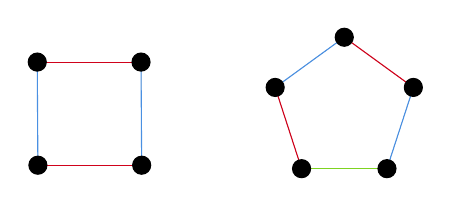
\begin{tikzpicture}[x=0.75pt,y=0.75pt,yscale=-1,xscale=1]
%uncomment if require: \path (0,175); %set diagram left start at 0, and has height of 175

%Straight Lines [id:da5818584723093488] 
\draw [color={rgb, 255:red, 74; green, 144; blue, 226 }  ,draw opacity=1 ][fill={rgb, 255:red, 0; green, 0; blue, 0 }  ,fill opacity=1 ]   (324.35,68.53) -- (357.63,44.35) ;
%Straight Lines [id:da6438228712778113] 
\draw [color={rgb, 255:red, 208; green, 2; blue, 27 }  ,draw opacity=1 ][fill={rgb, 255:red, 0; green, 0; blue, 0 }  ,fill opacity=1 ]   (357.63,44.35) -- (390.92,68.53) ;
%Straight Lines [id:da20205210194403878] 
\draw [color={rgb, 255:red, 74; green, 144; blue, 226 }  ,draw opacity=1 ][fill={rgb, 255:red, 0; green, 0; blue, 0 }  ,fill opacity=1 ]   (390.92,68.53) -- (378.2,107.66) ;
%Straight Lines [id:da6484989597274065] 
\draw [color={rgb, 255:red, 208; green, 2; blue, 27 }  ,draw opacity=1 ][fill={rgb, 255:red, 0; green, 0; blue, 0 }  ,fill opacity=1 ]   (324.35,68.53) -- (337.06,107.66) ;
%Straight Lines [id:da44992676892252104] 
\draw [color={rgb, 255:red, 126; green, 211; blue, 33 }  ,draw opacity=1 ][fill={rgb, 255:red, 0; green, 0; blue, 0 }  ,fill opacity=1 ]   (337.06,107.66) -- (378.2,107.66) ;
%Straight Lines [id:da09765976020965883] 
\draw [color={rgb, 255:red, 74; green, 144; blue, 226 }  ,draw opacity=1 ][fill={rgb, 255:red, 0; green, 0; blue, 0 }  ,fill opacity=1 ]   (209.71,56.31) -- (210.02,106) ;
%Straight Lines [id:da28251783698025235] 
\draw [color={rgb, 255:red, 74; green, 144; blue, 226 }  ,draw opacity=1 ][fill={rgb, 255:red, 0; green, 0; blue, 0 }  ,fill opacity=1 ]   (259.71,56.31) -- (260.02,106) ;
%Straight Lines [id:da8378590398614684] 
\draw [color={rgb, 255:red, 208; green, 2; blue, 27 }  ,draw opacity=1 ][fill={rgb, 255:red, 0; green, 0; blue, 0 }  ,fill opacity=1 ]   (209.71,56.31) -- (259.71,56.31) ;
%Straight Lines [id:da9063001360903188] 
\draw [color={rgb, 255:red, 208; green, 2; blue, 27 }  ,draw opacity=1 ][fill={rgb, 255:red, 0; green, 0; blue, 0 }  ,fill opacity=1 ]   (210.02,106) -- (260.02,106) ;
%Shape: Ellipse [id:dp6280991583392747] 
\draw  [color={rgb, 255:red, 0; green, 0; blue, 0 }  ,draw opacity=1 ][fill={rgb, 255:red, 0; green, 0; blue, 0 }  ,fill opacity=1 ] (205.37,56.31) .. controls (205.37,53.91) and (207.31,51.96) .. (209.71,51.96) .. controls (212.11,51.96) and (214.06,53.91) .. (214.06,56.31) .. controls (214.06,58.71) and (212.11,60.65) .. (209.71,60.65) .. controls (207.31,60.65) and (205.37,58.71) .. (205.37,56.31) -- cycle ;
%Shape: Ellipse [id:dp043129038325385505] 
\draw  [color={rgb, 255:red, 0; green, 0; blue, 0 }  ,draw opacity=1 ][fill={rgb, 255:red, 0; green, 0; blue, 0 }  ,fill opacity=1 ] (255.37,56.31) .. controls (255.37,53.91) and (257.31,51.96) .. (259.71,51.96) .. controls (262.11,51.96) and (264.06,53.91) .. (264.06,56.31) .. controls (264.06,58.71) and (262.11,60.65) .. (259.71,60.65) .. controls (257.31,60.65) and (255.37,58.71) .. (255.37,56.31) -- cycle ;
%Shape: Ellipse [id:dp7561533247578217] 
\draw  [color={rgb, 255:red, 0; green, 0; blue, 0 }  ,draw opacity=1 ][fill={rgb, 255:red, 0; green, 0; blue, 0 }  ,fill opacity=1 ] (205.68,106) .. controls (205.68,103.6) and (207.62,101.65) .. (210.02,101.65) .. controls (212.42,101.65) and (214.37,103.6) .. (214.37,106) .. controls (214.37,108.4) and (212.42,110.35) .. (210.02,110.35) .. controls (207.62,110.35) and (205.68,108.4) .. (205.68,106) -- cycle ;
%Shape: Ellipse [id:dp11572730400136533] 
\draw  [color={rgb, 255:red, 0; green, 0; blue, 0 }  ,draw opacity=1 ][fill={rgb, 255:red, 0; green, 0; blue, 0 }  ,fill opacity=1 ] (255.68,106) .. controls (255.68,103.6) and (257.62,101.65) .. (260.02,101.65) .. controls (262.42,101.65) and (264.37,103.6) .. (264.37,106) .. controls (264.37,108.4) and (262.42,110.35) .. (260.02,110.35) .. controls (257.62,110.35) and (255.68,108.4) .. (255.68,106) -- cycle ;
%Shape: Ellipse [id:dp5280959434489964] 
\draw  [color={rgb, 255:red, 0; green, 0; blue, 0 }  ,draw opacity=1 ][fill={rgb, 255:red, 0; green, 0; blue, 0 }  ,fill opacity=1 ] (353.29,44.35) .. controls (353.29,41.95) and (355.23,40) .. (357.63,40) .. controls (360.03,40) and (361.98,41.95) .. (361.98,44.35) .. controls (361.98,46.74) and (360.03,48.69) .. (357.63,48.69) .. controls (355.23,48.69) and (353.29,46.74) .. (353.29,44.35) -- cycle ;
%Shape: Ellipse [id:dp41708758591960915] 
\draw  [color={rgb, 255:red, 0; green, 0; blue, 0 }  ,draw opacity=1 ][fill={rgb, 255:red, 0; green, 0; blue, 0 }  ,fill opacity=1 ] (320,68.53) .. controls (320,66.13) and (321.95,64.18) .. (324.35,64.18) .. controls (326.74,64.18) and (328.69,66.13) .. (328.69,68.53) .. controls (328.69,70.93) and (326.74,72.87) .. (324.35,72.87) .. controls (321.95,72.87) and (320,70.93) .. (320,68.53) -- cycle ;
%Shape: Ellipse [id:dp9100616052151284] 
\draw  [color={rgb, 255:red, 0; green, 0; blue, 0 }  ,draw opacity=1 ][fill={rgb, 255:red, 0; green, 0; blue, 0 }  ,fill opacity=1 ] (332.71,107.66) .. controls (332.71,105.26) and (334.66,103.32) .. (337.06,103.32) .. controls (339.46,103.32) and (341.4,105.26) .. (341.4,107.66) .. controls (341.4,110.06) and (339.46,112.01) .. (337.06,112.01) .. controls (334.66,112.01) and (332.71,110.06) .. (332.71,107.66) -- cycle ;
%Shape: Ellipse [id:dp7916046119617446] 
\draw  [color={rgb, 255:red, 0; green, 0; blue, 0 }  ,draw opacity=1 ][fill={rgb, 255:red, 0; green, 0; blue, 0 }  ,fill opacity=1 ] (373.86,107.66) .. controls (373.86,105.26) and (375.8,103.32) .. (378.2,103.32) .. controls (380.6,103.32) and (382.55,105.26) .. (382.55,107.66) .. controls (382.55,110.06) and (380.6,112.01) .. (378.2,112.01) .. controls (375.8,112.01) and (373.86,110.06) .. (373.86,107.66) -- cycle ;
%Shape: Ellipse [id:dp9430238588703118] 
\draw  [color={rgb, 255:red, 0; green, 0; blue, 0 }  ,draw opacity=1 ][fill={rgb, 255:red, 0; green, 0; blue, 0 }  ,fill opacity=1 ] (386.57,68.53) .. controls (386.57,66.13) and (388.52,64.18) .. (390.92,64.18) .. controls (393.32,64.18) and (395.26,66.13) .. (395.26,68.53) .. controls (395.26,70.93) and (393.32,72.87) .. (390.92,72.87) .. controls (388.52,72.87) and (386.57,70.93) .. (386.57,68.53) -- cycle ;




\end{tikzpicture}

	\end{center}
The Petersen graph $G$ has $\chi'(G) = 4$.
\begin{center}
	

\tikzset{every picture/.style={line width=0.75pt}} %set default line width to 0.75pt        

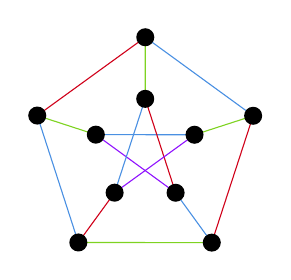
\begin{tikzpicture}[x=0.75pt,y=0.75pt,yscale=-1,xscale=1]
%uncomment if require: \path (0,244); %set diagram left start at 0, and has height of 244

%Shape: Regular Polygon [id:dp16247621401763546] 
\draw  [draw opacity=0] (305.27,98.38) -- (296.16,126.32) -- (266.77,126.29) -- (257.72,98.33) -- (281.51,81.08) -- cycle ;
%Straight Lines [id:da893034179191285] 
\draw [color={rgb, 255:red, 74; green, 144; blue, 226 }  ,draw opacity=1 ]   (257.72,98.33) -- (305.27,98.38) ;
%Straight Lines [id:da660375333141121] 
\draw [color={rgb, 255:red, 208; green, 2; blue, 27 }  ,draw opacity=1 ]   (281.51,81.08) -- (296.16,126.32) ;
%Straight Lines [id:da20428445610159474] 
\draw [color={rgb, 255:red, 144; green, 19; blue, 254 }  ,draw opacity=1 ]   (305.27,98.38) -- (266.77,126.29) ;
%Straight Lines [id:da8709633259609025] 
\draw [color={rgb, 255:red, 144; green, 19; blue, 254 }  ,draw opacity=1 ]   (257.72,98.33) -- (296.16,126.32) ;
%Straight Lines [id:da44608612111926593] 
\draw [color={rgb, 255:red, 74; green, 144; blue, 226 }  ,draw opacity=1 ]   (281.51,81.08) -- (266.77,126.29) ;
%Straight Lines [id:da7715209790387976] 
\draw [color={rgb, 255:red, 126; green, 211; blue, 33 }  ,draw opacity=1 ]   (229.5,89.13) -- (257.72,98.33) ;
%Straight Lines [id:da7455142272486954] 
\draw [color={rgb, 255:red, 126; green, 211; blue, 33 }  ,draw opacity=1 ]   (281.51,81.08) -- (281.54,51.4) ;
%Straight Lines [id:da02789801208249232] 
\draw [color={rgb, 255:red, 126; green, 211; blue, 33 }  ,draw opacity=1 ]   (333.51,89.24) -- (305.27,98.38) ;
%Straight Lines [id:da005285258139439142] 
\draw [color={rgb, 255:red, 74; green, 144; blue, 226 }  ,draw opacity=1 ]   (313.58,150.35) -- (296.16,126.32) ;
%Straight Lines [id:da49353402840189853] 
\draw [color={rgb, 255:red, 208; green, 2; blue, 27 }  ,draw opacity=1 ]   (249.3,150.29) -- (266.77,126.29) ;
%Straight Lines [id:da7550778902430247] 
\draw [color={rgb, 255:red, 74; green, 144; blue, 226 }  ,draw opacity=1 ]   (281.54,51.4) -- (333.51,89.24) ;
%Straight Lines [id:da18269980385284001] 
\draw [color={rgb, 255:red, 208; green, 2; blue, 27 }  ,draw opacity=1 ]   (313.58,150.35) -- (333.51,89.24) ;
%Straight Lines [id:da5454729619903863] 
\draw [color={rgb, 255:red, 74; green, 144; blue, 226 }  ,draw opacity=1 ]   (249.3,150.29) -- (229.5,89.13) ;
%Straight Lines [id:da8485573440500561] 
\draw [color={rgb, 255:red, 208; green, 2; blue, 27 }  ,draw opacity=1 ]   (229.5,89.13) -- (281.54,51.4) ;
%Straight Lines [id:da35360141311203563] 
\draw [color={rgb, 255:red, 126; green, 211; blue, 33 }  ,draw opacity=1 ]   (249.3,150.29) -- (313.58,150.35) ;
%Shape: Ellipse [id:dp35124028454844947] 
\draw  [draw opacity=0][fill={rgb, 255:red, 0; green, 0; blue, 0 }  ,fill opacity=1 ] (277.17,81.08) .. controls (277.17,78.68) and (279.11,76.74) .. (281.51,76.74) .. controls (283.91,76.74) and (285.86,78.68) .. (285.86,81.08) .. controls (285.86,83.48) and (283.91,85.43) .. (281.51,85.43) .. controls (279.11,85.43) and (277.17,83.48) .. (277.17,81.08) -- cycle ;
%Shape: Ellipse [id:dp4821028647771225] 
\draw  [draw opacity=0][fill={rgb, 255:red, 0; green, 0; blue, 0 }  ,fill opacity=1 ] (253.37,98.33) .. controls (253.37,95.93) and (255.32,93.99) .. (257.72,93.99) .. controls (260.12,93.99) and (262.06,95.93) .. (262.06,98.33) .. controls (262.06,100.73) and (260.12,102.68) .. (257.72,102.68) .. controls (255.32,102.68) and (253.37,100.73) .. (253.37,98.33) -- cycle ;
%Shape: Ellipse [id:dp19844657244731556] 
\draw  [draw opacity=0][fill={rgb, 255:red, 0; green, 0; blue, 0 }  ,fill opacity=1 ] (262.42,126.29) .. controls (262.42,123.89) and (264.37,121.95) .. (266.77,121.95) .. controls (269.17,121.95) and (271.11,123.89) .. (271.11,126.29) .. controls (271.11,128.69) and (269.17,130.64) .. (266.77,130.64) .. controls (264.37,130.64) and (262.42,128.69) .. (262.42,126.29) -- cycle ;
%Shape: Ellipse [id:dp6691944544969051] 
\draw  [draw opacity=0][fill={rgb, 255:red, 0; green, 0; blue, 0 }  ,fill opacity=1 ] (291.81,126.32) .. controls (291.81,123.93) and (293.76,121.98) .. (296.16,121.98) .. controls (298.56,121.98) and (300.5,123.93) .. (300.5,126.32) .. controls (300.5,128.72) and (298.56,130.67) .. (296.16,130.67) .. controls (293.76,130.67) and (291.81,128.72) .. (291.81,126.32) -- cycle ;
%Shape: Ellipse [id:dp9762766192339163] 
\draw  [draw opacity=0][fill={rgb, 255:red, 0; green, 0; blue, 0 }  ,fill opacity=1 ] (300.92,98.38) .. controls (300.92,95.98) and (302.87,94.04) .. (305.27,94.04) .. controls (307.67,94.04) and (309.61,95.98) .. (309.61,98.38) .. controls (309.61,100.78) and (307.67,102.73) .. (305.27,102.73) .. controls (302.87,102.73) and (300.92,100.78) .. (300.92,98.38) -- cycle ;
%Shape: Ellipse [id:dp20883567956782512] 
\draw  [draw opacity=0][fill={rgb, 255:red, 0; green, 0; blue, 0 }  ,fill opacity=1 ] (225.15,89.13) .. controls (225.15,86.73) and (227.1,84.79) .. (229.5,84.79) .. controls (231.9,84.79) and (233.84,86.73) .. (233.84,89.13) .. controls (233.84,91.53) and (231.9,93.48) .. (229.5,93.48) .. controls (227.1,93.48) and (225.15,91.53) .. (225.15,89.13) -- cycle ;
%Shape: Ellipse [id:dp5756340573590069] 
\draw  [draw opacity=0][fill={rgb, 255:red, 0; green, 0; blue, 0 }  ,fill opacity=1 ] (277.2,51.4) .. controls (277.2,49) and (279.14,47.06) .. (281.54,47.06) .. controls (283.94,47.06) and (285.89,49) .. (285.89,51.4) .. controls (285.89,53.8) and (283.94,55.75) .. (281.54,55.75) .. controls (279.14,55.75) and (277.2,53.8) .. (277.2,51.4) -- cycle ;
%Shape: Ellipse [id:dp8418291390960153] 
\draw  [draw opacity=0][fill={rgb, 255:red, 0; green, 0; blue, 0 }  ,fill opacity=1 ] (329.16,89.24) .. controls (329.16,86.84) and (331.11,84.9) .. (333.51,84.9) .. controls (335.91,84.9) and (337.85,86.84) .. (337.85,89.24) .. controls (337.85,91.64) and (335.91,93.59) .. (333.51,93.59) .. controls (331.11,93.59) and (329.16,91.64) .. (329.16,89.24) -- cycle ;
%Shape: Ellipse [id:dp4698372731071758] 
\draw  [draw opacity=0][fill={rgb, 255:red, 0; green, 0; blue, 0 }  ,fill opacity=1 ] (309.23,150.35) .. controls (309.23,147.95) and (311.18,146.01) .. (313.58,146.01) .. controls (315.98,146.01) and (317.92,147.95) .. (317.92,150.35) .. controls (317.92,152.75) and (315.98,154.7) .. (313.58,154.7) .. controls (311.18,154.7) and (309.23,152.75) .. (309.23,150.35) -- cycle ;
%Shape: Ellipse [id:dp47034805208827146] 
\draw  [draw opacity=0][fill={rgb, 255:red, 0; green, 0; blue, 0 }  ,fill opacity=1 ] (244.95,150.29) .. controls (244.95,147.89) and (246.9,145.94) .. (249.3,145.94) .. controls (251.7,145.94) and (253.64,147.89) .. (253.64,150.29) .. controls (253.64,152.69) and (251.7,154.63) .. (249.3,154.63) .. controls (246.9,154.63) and (244.95,152.69) .. (244.95,150.29) -- cycle ;




\end{tikzpicture}
\end{center} 
\end{example}

In contrast to the chromatic number, it is much easier to get a handle on the edge chromatic number, as we will see in the following theorem.


\begin{theorem}[Vizing's Theorem]
	Let $G$ be a graph. Then $\Delta(G) \leq \chi'(G) \leq \Delta(G) + 1$.
\end{theorem}
\begin{proof}
	We proceed by induction on $e(G)$. The basis step is trivial, then for the inductive step we are given a graph $G$, and let's assume for a contradiction that $\chi'(G) > \Delta + 1$.

	By induction, $G - e$ has a $\Delta + 1$ colouring, so let's write $e = xy$ with $x \neq y \in G$. We define vertices $y_1, \dots, y_k$ inductively by setting $y_1 = y$. Now assume $y_1, \dots, y_t$ are defined, and the colours missing from $y_1, \dots, y_t$ are $c_1, \dots, c_t$ respectively. Then if $c_t \not \in \{c_1, \dots, c_{t - 1}\}$, then let $y_{t + 1}$ be so that $xy_{y + 1}$ receives colour $c_t$.
	Note that such a vertex exists as otherwise we could recolour $xy_1$ with $c_1$, $xy_2$  with $c_2$, and so on until $x y_t$ is with $c_t$, to obtain a $\Delta + 1$ colouring, which is a  contradiction.

	Now if $c_t \in \{c_1, \dots, c_{t - 1}\}$, then stop. Say we stop after $k$ steps, so I have defined $y_1, \dots, y_k$ with missing colours $c_1, \dots, c_k$ and $c_k = c_i$ for some $i < k$. We may assume that $i = 1$ (otherwise uncolour the edge $xy_i$ and recolour $xy_1$ with $c_1$, and so on until $xy_{i - 1}$ with $c_{i - 1}$).

	Let's call the colour missing at $x$, $c_0$. Consider the $\{c_0, c_1\}$ component $C$, containing $y_1$. If $x \not \in C$, then we can flip colours on $C$ so that $c_0$ is missing at $y_1$, then colour $xy_1$ with $c_0$. Likewise, the $\{c_0, c_1\}$-component containing $y_k$ must contain $x$, as otherwise we flip colours on this component so that the colour $c_0$ is missing at $y_k$. Then recolour $xy_k$ to $c_0$ and $xy_i$ to $c_i$ for $i < k$.

	Thus $x, y_1, y_k \in C$, the $\{c_0, c_1\}$-component. But this is impossible since $x, y_1, y_k$ all have one of the colours $\{c_0, c_1\}$ missing, thus $d_C(x), d_C(y_1), d_C(y_k) \leq 1$. But this is is impossible for a path or cycle.
\end{proof}

\begin{remark}
	This theorem is \emph{not} true if we generalize to multigraphs, which are graphs that have multiple edges between vertices.
\end{remark}

\section{Extremal Graph Theory}

Welcome to the section on extremal graph theory, where we think about problems involving things with an `extreme' flavour.

\subsection{Eulerian Circuits and Hamiltonian Cycles}

We are going to begin our chapter on extremal graph theory with something that's not \emph{really} extremal graph theory. Still, it will lead us nicely into the more extreme parts of this chapter and the course. Let's state a definition.

\begin{definition}[Eulerian Circuit]
	An \vocab{Eulerian circuit} is a circuit in a graph $G$ that crosses each edge exactly once. If a $G$ has an Eulerian circuit, we say that the graph is \vocab{Eulerian}.
\end{definition}

\begin{center}
	

\tikzset{every picture/.style={line width=0.75pt}} %set default line width to 0.75pt        

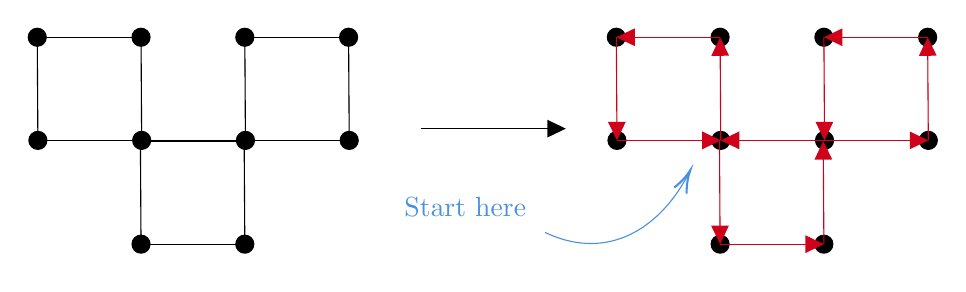
\begin{tikzpicture}[x=0.75pt,y=0.75pt,yscale=-1,xscale=1]
%uncomment if require: \path (0,175); %set diagram left start at 0, and has height of 175

%Straight Lines [id:da7603262804371462] 
\draw [color={rgb, 255:red, 0; green, 0; blue, 0 }  ,draw opacity=1 ][fill={rgb, 255:red, 0; green, 0; blue, 0 }  ,fill opacity=1 ]   (45.35,35.96) -- (45.65,85.65) ;
%Straight Lines [id:da9822428602979119] 
\draw [color={rgb, 255:red, 0; green, 0; blue, 0 }  ,draw opacity=1 ][fill={rgb, 255:red, 0; green, 0; blue, 0 }  ,fill opacity=1 ]   (95.35,35.96) -- (95.65,85.65) ;
%Straight Lines [id:da10643781966910082] 
\draw [color={rgb, 255:red, 0; green, 0; blue, 0 }  ,draw opacity=1 ][fill={rgb, 255:red, 0; green, 0; blue, 0 }  ,fill opacity=1 ]   (45.35,35.96) -- (95.35,35.96) ;
%Straight Lines [id:da562491639434787] 
\draw [color={rgb, 255:red, 0; green, 0; blue, 0 }  ,draw opacity=1 ][fill={rgb, 255:red, 0; green, 0; blue, 0 }  ,fill opacity=1 ]   (45.65,85.65) -- (95.65,85.65) ;
%Shape: Ellipse [id:dp4179759025968104] 
\draw  [color={rgb, 255:red, 0; green, 0; blue, 0 }  ,draw opacity=1 ][fill={rgb, 255:red, 0; green, 0; blue, 0 }  ,fill opacity=1 ] (41,35.96) .. controls (41,33.57) and (42.95,31.62) .. (45.35,31.62) .. controls (47.74,31.62) and (49.69,33.57) .. (49.69,35.96) .. controls (49.69,38.36) and (47.74,40.31) .. (45.35,40.31) .. controls (42.95,40.31) and (41,38.36) .. (41,35.96) -- cycle ;
%Shape: Ellipse [id:dp485136849858802] 
\draw  [color={rgb, 255:red, 0; green, 0; blue, 0 }  ,draw opacity=1 ][fill={rgb, 255:red, 0; green, 0; blue, 0 }  ,fill opacity=1 ] (91,35.96) .. controls (91,33.57) and (92.95,31.62) .. (95.35,31.62) .. controls (97.74,31.62) and (99.69,33.57) .. (99.69,35.96) .. controls (99.69,38.36) and (97.74,40.31) .. (95.35,40.31) .. controls (92.95,40.31) and (91,38.36) .. (91,35.96) -- cycle ;
%Shape: Ellipse [id:dp7959472896183609] 
\draw  [color={rgb, 255:red, 0; green, 0; blue, 0 }  ,draw opacity=1 ][fill={rgb, 255:red, 0; green, 0; blue, 0 }  ,fill opacity=1 ] (41.31,85.65) .. controls (41.31,83.26) and (43.26,81.31) .. (45.65,81.31) .. controls (48.05,81.31) and (50,83.26) .. (50,85.65) .. controls (50,88.05) and (48.05,90) .. (45.65,90) .. controls (43.26,90) and (41.31,88.05) .. (41.31,85.65) -- cycle ;
%Straight Lines [id:da4638832571081428] 
\draw [color={rgb, 255:red, 0; green, 0; blue, 0 }  ,draw opacity=1 ][fill={rgb, 255:red, 0; green, 0; blue, 0 }  ,fill opacity=1 ]   (95.04,85.96) -- (95.35,135.65) ;
%Straight Lines [id:da34603627442334806] 
\draw [color={rgb, 255:red, 0; green, 0; blue, 0 }  ,draw opacity=1 ][fill={rgb, 255:red, 0; green, 0; blue, 0 }  ,fill opacity=1 ]   (145.04,85.96) -- (145.35,135.65) ;
%Straight Lines [id:da1846224756159932] 
\draw [color={rgb, 255:red, 0; green, 0; blue, 0 }  ,draw opacity=1 ][fill={rgb, 255:red, 0; green, 0; blue, 0 }  ,fill opacity=1 ]   (95.04,85.96) -- (145.04,85.96) ;
%Straight Lines [id:da49009857284037595] 
\draw [color={rgb, 255:red, 0; green, 0; blue, 0 }  ,draw opacity=1 ][fill={rgb, 255:red, 0; green, 0; blue, 0 }  ,fill opacity=1 ]   (95.35,135.65) -- (145.35,135.65) ;
%Shape: Ellipse [id:dp7737699621871421] 
\draw  [color={rgb, 255:red, 0; green, 0; blue, 0 }  ,draw opacity=1 ][fill={rgb, 255:red, 0; green, 0; blue, 0 }  ,fill opacity=1 ] (91,135.65) .. controls (91,133.26) and (92.95,131.31) .. (95.35,131.31) .. controls (97.74,131.31) and (99.69,133.26) .. (99.69,135.65) .. controls (99.69,138.05) and (97.74,140) .. (95.35,140) .. controls (92.95,140) and (91,138.05) .. (91,135.65) -- cycle ;
%Shape: Ellipse [id:dp3911078350081243] 
\draw  [color={rgb, 255:red, 0; green, 0; blue, 0 }  ,draw opacity=1 ][fill={rgb, 255:red, 0; green, 0; blue, 0 }  ,fill opacity=1 ] (141,135.65) .. controls (141,133.26) and (142.95,131.31) .. (145.35,131.31) .. controls (147.74,131.31) and (149.69,133.26) .. (149.69,135.65) .. controls (149.69,138.05) and (147.74,140) .. (145.35,140) .. controls (142.95,140) and (141,138.05) .. (141,135.65) -- cycle ;
%Straight Lines [id:da3452664170004852] 
\draw [color={rgb, 255:red, 0; green, 0; blue, 0 }  ,draw opacity=1 ][fill={rgb, 255:red, 0; green, 0; blue, 0 }  ,fill opacity=1 ]   (145.35,35.96) -- (145.65,85.65) ;
%Straight Lines [id:da46801263026426254] 
\draw [color={rgb, 255:red, 0; green, 0; blue, 0 }  ,draw opacity=1 ][fill={rgb, 255:red, 0; green, 0; blue, 0 }  ,fill opacity=1 ]   (195.35,35.96) -- (195.65,85.65) ;
%Straight Lines [id:da5435544765028092] 
\draw [color={rgb, 255:red, 0; green, 0; blue, 0 }  ,draw opacity=1 ][fill={rgb, 255:red, 0; green, 0; blue, 0 }  ,fill opacity=1 ]   (145.35,35.96) -- (195.35,35.96) ;
%Straight Lines [id:da2115803748127968] 
\draw [color={rgb, 255:red, 0; green, 0; blue, 0 }  ,draw opacity=1 ][fill={rgb, 255:red, 0; green, 0; blue, 0 }  ,fill opacity=1 ]   (145.65,85.65) -- (195.65,85.65) ;
%Shape: Ellipse [id:dp11383225146528286] 
\draw  [color={rgb, 255:red, 0; green, 0; blue, 0 }  ,draw opacity=1 ][fill={rgb, 255:red, 0; green, 0; blue, 0 }  ,fill opacity=1 ] (141,35.96) .. controls (141,33.57) and (142.95,31.62) .. (145.35,31.62) .. controls (147.74,31.62) and (149.69,33.57) .. (149.69,35.96) .. controls (149.69,38.36) and (147.74,40.31) .. (145.35,40.31) .. controls (142.95,40.31) and (141,38.36) .. (141,35.96) -- cycle ;
%Shape: Ellipse [id:dp9998049000953178] 
\draw  [color={rgb, 255:red, 0; green, 0; blue, 0 }  ,draw opacity=1 ][fill={rgb, 255:red, 0; green, 0; blue, 0 }  ,fill opacity=1 ] (191,35.96) .. controls (191,33.57) and (192.95,31.62) .. (195.35,31.62) .. controls (197.74,31.62) and (199.69,33.57) .. (199.69,35.96) .. controls (199.69,38.36) and (197.74,40.31) .. (195.35,40.31) .. controls (192.95,40.31) and (191,38.36) .. (191,35.96) -- cycle ;
%Shape: Ellipse [id:dp3910356973019917] 
\draw  [color={rgb, 255:red, 0; green, 0; blue, 0 }  ,draw opacity=1 ][fill={rgb, 255:red, 0; green, 0; blue, 0 }  ,fill opacity=1 ] (141.31,85.65) .. controls (141.31,83.26) and (143.26,81.31) .. (145.65,81.31) .. controls (148.05,81.31) and (150,83.26) .. (150,85.65) .. controls (150,88.05) and (148.05,90) .. (145.65,90) .. controls (143.26,90) and (141.31,88.05) .. (141.31,85.65) -- cycle ;
%Shape: Ellipse [id:dp6400303577331324] 
\draw  [color={rgb, 255:red, 0; green, 0; blue, 0 }  ,draw opacity=1 ][fill={rgb, 255:red, 0; green, 0; blue, 0 }  ,fill opacity=1 ] (191.31,85.65) .. controls (191.31,83.26) and (193.26,81.31) .. (195.65,81.31) .. controls (198.05,81.31) and (200,83.26) .. (200,85.65) .. controls (200,88.05) and (198.05,90) .. (195.65,90) .. controls (193.26,90) and (191.31,88.05) .. (191.31,85.65) -- cycle ;
%Shape: Ellipse [id:dp5267785678494632] 
\draw  [color={rgb, 255:red, 0; green, 0; blue, 0 }  ,draw opacity=1 ][fill={rgb, 255:red, 0; green, 0; blue, 0 }  ,fill opacity=1 ] (91.31,85.65) .. controls (91.31,83.26) and (93.26,81.31) .. (95.65,81.31) .. controls (98.05,81.31) and (100,83.26) .. (100,85.65) .. controls (100,88.05) and (98.05,90) .. (95.65,90) .. controls (93.26,90) and (91.31,88.05) .. (91.31,85.65) -- cycle ;
%Shape: Ellipse [id:dp8401978184996424] 
\draw  [color={rgb, 255:red, 0; green, 0; blue, 0 }  ,draw opacity=1 ][fill={rgb, 255:red, 0; green, 0; blue, 0 }  ,fill opacity=1 ] (320,35.96) .. controls (320,33.57) and (321.95,31.62) .. (324.35,31.62) .. controls (326.74,31.62) and (328.69,33.57) .. (328.69,35.96) .. controls (328.69,38.36) and (326.74,40.31) .. (324.35,40.31) .. controls (321.95,40.31) and (320,38.36) .. (320,35.96) -- cycle ;
%Shape: Ellipse [id:dp1719081834686207] 
\draw  [color={rgb, 255:red, 0; green, 0; blue, 0 }  ,draw opacity=1 ][fill={rgb, 255:red, 0; green, 0; blue, 0 }  ,fill opacity=1 ] (370,35.96) .. controls (370,33.57) and (371.95,31.62) .. (374.35,31.62) .. controls (376.74,31.62) and (378.69,33.57) .. (378.69,35.96) .. controls (378.69,38.36) and (376.74,40.31) .. (374.35,40.31) .. controls (371.95,40.31) and (370,38.36) .. (370,35.96) -- cycle ;
%Shape: Ellipse [id:dp5581136438440253] 
\draw  [color={rgb, 255:red, 0; green, 0; blue, 0 }  ,draw opacity=1 ][fill={rgb, 255:red, 0; green, 0; blue, 0 }  ,fill opacity=1 ] (320.31,85.65) .. controls (320.31,83.26) and (322.26,81.31) .. (324.65,81.31) .. controls (327.05,81.31) and (329,83.26) .. (329,85.65) .. controls (329,88.05) and (327.05,90) .. (324.65,90) .. controls (322.26,90) and (320.31,88.05) .. (320.31,85.65) -- cycle ;
%Shape: Ellipse [id:dp7345098827105483] 
\draw  [color={rgb, 255:red, 0; green, 0; blue, 0 }  ,draw opacity=1 ][fill={rgb, 255:red, 0; green, 0; blue, 0 }  ,fill opacity=1 ] (370,135.65) .. controls (370,133.26) and (371.95,131.31) .. (374.35,131.31) .. controls (376.74,131.31) and (378.69,133.26) .. (378.69,135.65) .. controls (378.69,138.05) and (376.74,140) .. (374.35,140) .. controls (371.95,140) and (370,138.05) .. (370,135.65) -- cycle ;
%Shape: Ellipse [id:dp12225853858737912] 
\draw  [color={rgb, 255:red, 0; green, 0; blue, 0 }  ,draw opacity=1 ][fill={rgb, 255:red, 0; green, 0; blue, 0 }  ,fill opacity=1 ] (420,135.65) .. controls (420,133.26) and (421.95,131.31) .. (424.35,131.31) .. controls (426.74,131.31) and (428.69,133.26) .. (428.69,135.65) .. controls (428.69,138.05) and (426.74,140) .. (424.35,140) .. controls (421.95,140) and (420,138.05) .. (420,135.65) -- cycle ;
%Shape: Ellipse [id:dp44237158127089693] 
\draw  [color={rgb, 255:red, 0; green, 0; blue, 0 }  ,draw opacity=1 ][fill={rgb, 255:red, 0; green, 0; blue, 0 }  ,fill opacity=1 ] (420,35.96) .. controls (420,33.57) and (421.95,31.62) .. (424.35,31.62) .. controls (426.74,31.62) and (428.69,33.57) .. (428.69,35.96) .. controls (428.69,38.36) and (426.74,40.31) .. (424.35,40.31) .. controls (421.95,40.31) and (420,38.36) .. (420,35.96) -- cycle ;
%Shape: Ellipse [id:dp29018716879103434] 
\draw  [color={rgb, 255:red, 0; green, 0; blue, 0 }  ,draw opacity=1 ][fill={rgb, 255:red, 0; green, 0; blue, 0 }  ,fill opacity=1 ] (470,35.96) .. controls (470,33.57) and (471.95,31.62) .. (474.35,31.62) .. controls (476.74,31.62) and (478.69,33.57) .. (478.69,35.96) .. controls (478.69,38.36) and (476.74,40.31) .. (474.35,40.31) .. controls (471.95,40.31) and (470,38.36) .. (470,35.96) -- cycle ;
%Shape: Ellipse [id:dp7704124674085753] 
\draw  [color={rgb, 255:red, 0; green, 0; blue, 0 }  ,draw opacity=1 ][fill={rgb, 255:red, 0; green, 0; blue, 0 }  ,fill opacity=1 ] (420.31,85.65) .. controls (420.31,83.26) and (422.26,81.31) .. (424.65,81.31) .. controls (427.05,81.31) and (429,83.26) .. (429,85.65) .. controls (429,88.05) and (427.05,90) .. (424.65,90) .. controls (422.26,90) and (420.31,88.05) .. (420.31,85.65) -- cycle ;
%Shape: Ellipse [id:dp8213993184652387] 
\draw  [color={rgb, 255:red, 0; green, 0; blue, 0 }  ,draw opacity=1 ][fill={rgb, 255:red, 0; green, 0; blue, 0 }  ,fill opacity=1 ] (470.31,85.65) .. controls (470.31,83.26) and (472.26,81.31) .. (474.65,81.31) .. controls (477.05,81.31) and (479,83.26) .. (479,85.65) .. controls (479,88.05) and (477.05,90) .. (474.65,90) .. controls (472.26,90) and (470.31,88.05) .. (470.31,85.65) -- cycle ;
%Shape: Ellipse [id:dp4921848947529245] 
\draw  [color={rgb, 255:red, 0; green, 0; blue, 0 }  ,draw opacity=1 ][fill={rgb, 255:red, 0; green, 0; blue, 0 }  ,fill opacity=1 ] (370.31,85.65) .. controls (370.31,83.26) and (372.26,81.31) .. (374.65,81.31) .. controls (377.05,81.31) and (379,83.26) .. (379,85.65) .. controls (379,88.05) and (377.05,90) .. (374.65,90) .. controls (372.26,90) and (370.31,88.05) .. (370.31,85.65) -- cycle ;
%Straight Lines [id:da1013385817733623] 
\draw [color={rgb, 255:red, 208; green, 2; blue, 27 }  ,draw opacity=1 ][fill={rgb, 255:red, 0; green, 0; blue, 0 }  ,fill opacity=1 ]   (324.35,35.96) -- (324.64,82.66) ;
\draw [shift={(324.65,85.65)}, rotate = 269.64] [fill={rgb, 255:red, 208; green, 2; blue, 27 }  ,fill opacity=1 ][line width=0.08]  [draw opacity=0] (8.93,-4.29) -- (0,0) -- (8.93,4.29) -- cycle    ;
%Straight Lines [id:da005494661969509096] 
\draw [color={rgb, 255:red, 208; green, 2; blue, 27 }  ,draw opacity=1 ][fill={rgb, 255:red, 0; green, 0; blue, 0 }  ,fill opacity=1 ]   (374.36,38.96) -- (374.65,85.65) ;
\draw [shift={(374.35,35.96)}, rotate = 89.64] [fill={rgb, 255:red, 208; green, 2; blue, 27 }  ,fill opacity=1 ][line width=0.08]  [draw opacity=0] (8.93,-4.29) -- (0,0) -- (8.93,4.29) -- cycle    ;
%Straight Lines [id:da10541466696614843] 
\draw [color={rgb, 255:red, 208; green, 2; blue, 27 }  ,draw opacity=1 ][fill={rgb, 255:red, 0; green, 0; blue, 0 }  ,fill opacity=1 ]   (327.35,35.96) -- (374.35,35.96) ;
\draw [shift={(324.35,35.96)}, rotate = 0] [fill={rgb, 255:red, 208; green, 2; blue, 27 }  ,fill opacity=1 ][line width=0.08]  [draw opacity=0] (8.93,-4.29) -- (0,0) -- (8.93,4.29) -- cycle    ;
%Straight Lines [id:da7846430990397626] 
\draw [color={rgb, 255:red, 208; green, 2; blue, 27 }  ,draw opacity=1 ][fill={rgb, 255:red, 0; green, 0; blue, 0 }  ,fill opacity=1 ]   (324.65,85.65) -- (371.65,85.65) ;
\draw [shift={(374.65,85.65)}, rotate = 180] [fill={rgb, 255:red, 208; green, 2; blue, 27 }  ,fill opacity=1 ][line width=0.08]  [draw opacity=0] (8.93,-4.29) -- (0,0) -- (8.93,4.29) -- cycle    ;
%Straight Lines [id:da00408066546359398] 
\draw [color={rgb, 255:red, 208; green, 2; blue, 27 }  ,draw opacity=1 ][fill={rgb, 255:red, 0; green, 0; blue, 0 }  ,fill opacity=1 ]   (374.04,85.96) -- (374.33,132.66) ;
\draw [shift={(374.35,135.65)}, rotate = 269.64] [fill={rgb, 255:red, 208; green, 2; blue, 27 }  ,fill opacity=1 ][line width=0.08]  [draw opacity=0] (8.93,-4.29) -- (0,0) -- (8.93,4.29) -- cycle    ;
%Straight Lines [id:da6751276547305484] 
\draw [color={rgb, 255:red, 208; green, 2; blue, 27 }  ,draw opacity=1 ][fill={rgb, 255:red, 0; green, 0; blue, 0 }  ,fill opacity=1 ]   (424.05,88.96) -- (424.35,135.65) ;
\draw [shift={(424.04,85.96)}, rotate = 89.64] [fill={rgb, 255:red, 208; green, 2; blue, 27 }  ,fill opacity=1 ][line width=0.08]  [draw opacity=0] (8.93,-4.29) -- (0,0) -- (8.93,4.29) -- cycle    ;
%Straight Lines [id:da8327010536524962] 
\draw [color={rgb, 255:red, 208; green, 2; blue, 27 }  ,draw opacity=1 ][fill={rgb, 255:red, 0; green, 0; blue, 0 }  ,fill opacity=1 ]   (377.65,85.65) -- (424.65,85.65) ;
\draw [shift={(374.65,85.65)}, rotate = 0] [fill={rgb, 255:red, 208; green, 2; blue, 27 }  ,fill opacity=1 ][line width=0.08]  [draw opacity=0] (8.93,-4.29) -- (0,0) -- (8.93,4.29) -- cycle    ;
%Straight Lines [id:da9196141405621421] 
\draw [color={rgb, 255:red, 208; green, 2; blue, 27 }  ,draw opacity=1 ][fill={rgb, 255:red, 0; green, 0; blue, 0 }  ,fill opacity=1 ]   (374.35,135.65) -- (421.35,135.65) ;
\draw [shift={(424.35,135.65)}, rotate = 180] [fill={rgb, 255:red, 208; green, 2; blue, 27 }  ,fill opacity=1 ][line width=0.08]  [draw opacity=0] (8.93,-4.29) -- (0,0) -- (8.93,4.29) -- cycle    ;
%Straight Lines [id:da6400080036802588] 
\draw [color={rgb, 255:red, 208; green, 2; blue, 27 }  ,draw opacity=1 ][fill={rgb, 255:red, 0; green, 0; blue, 0 }  ,fill opacity=1 ]   (424.35,35.96) -- (424.64,82.66) ;
\draw [shift={(424.65,85.65)}, rotate = 269.64] [fill={rgb, 255:red, 208; green, 2; blue, 27 }  ,fill opacity=1 ][line width=0.08]  [draw opacity=0] (8.93,-4.29) -- (0,0) -- (8.93,4.29) -- cycle    ;
%Straight Lines [id:da8049761624402324] 
\draw [color={rgb, 255:red, 208; green, 2; blue, 27 }  ,draw opacity=1 ][fill={rgb, 255:red, 0; green, 0; blue, 0 }  ,fill opacity=1 ]   (474.36,38.96) -- (474.65,85.65) ;
\draw [shift={(474.35,35.96)}, rotate = 89.64] [fill={rgb, 255:red, 208; green, 2; blue, 27 }  ,fill opacity=1 ][line width=0.08]  [draw opacity=0] (8.93,-4.29) -- (0,0) -- (8.93,4.29) -- cycle    ;
%Straight Lines [id:da4047081610001] 
\draw [color={rgb, 255:red, 208; green, 2; blue, 27 }  ,draw opacity=1 ][fill={rgb, 255:red, 0; green, 0; blue, 0 }  ,fill opacity=1 ]   (427.35,35.96) -- (474.35,35.96) ;
\draw [shift={(424.35,35.96)}, rotate = 0] [fill={rgb, 255:red, 208; green, 2; blue, 27 }  ,fill opacity=1 ][line width=0.08]  [draw opacity=0] (8.93,-4.29) -- (0,0) -- (8.93,4.29) -- cycle    ;
%Straight Lines [id:da7142459823691495] 
\draw [color={rgb, 255:red, 208; green, 2; blue, 27 }  ,draw opacity=1 ][fill={rgb, 255:red, 0; green, 0; blue, 0 }  ,fill opacity=1 ]   (424.65,85.65) -- (471.65,85.65) ;
\draw [shift={(474.65,85.65)}, rotate = 180] [fill={rgb, 255:red, 208; green, 2; blue, 27 }  ,fill opacity=1 ][line width=0.08]  [draw opacity=0] (8.93,-4.29) -- (0,0) -- (8.93,4.29) -- cycle    ;
%Straight Lines [id:da4435630532648108] 
\draw    (230,80) -- (297,80) ;
\draw [shift={(300,80)}, rotate = 180] [fill={rgb, 255:red, 0; green, 0; blue, 0 }  ][line width=0.08]  [draw opacity=0] (8.93,-4.29) -- (0,0) -- (8.93,4.29) -- cycle    ;
%Curve Lines [id:da8506229331842947] 
\draw [color={rgb, 255:red, 74; green, 144; blue, 226 }  ,draw opacity=1 ]   (290,130) .. controls (321.69,145.03) and (346.65,126.12) .. (359.24,101.51) ;
\draw [shift={(360,100)}, rotate = 475.96] [color={rgb, 255:red, 74; green, 144; blue, 226 }  ,draw opacity=1 ][line width=0.75]    (10.93,-3.29) .. controls (6.95,-1.4) and (3.31,-0.3) .. (0,0) .. controls (3.31,0.3) and (6.95,1.4) .. (10.93,3.29)   ;

% Text Node
\draw (221,112) node [anchor=north west][inner sep=0.75pt]  [color={rgb, 255:red, 74; green, 144; blue, 226 }  ,opacity=1 ] [align=left] {Start here};


\end{tikzpicture}

\end{center}

What's nice is that there is a straightforward characterisation of Eulerian graphs.

\begin{theorem}[Euler's Theorem]
	A connected graph has an Eulerian circuit if and only if every vertex has even degree.
\end{theorem}
\begin{proof}
	If a graph $G$ has an Eulerian circuit, then the degree of each vertex must be even. This is because a fixed vertex $x$ is entered and exited a fixed number of times.

	Now if each vertex of a graph $G$ has even degree, we will apply induction on $e(G)$. If $e(G) = 0$, then we are done. Now if $d(x) \geq 1$ for all vertices $x$, then $d(x) \geq 2$, and $G$ contains a cycle $C$. Define $G' = G - E(C)$. Let $G_1, \dots, G_k$ be the components of $G'$. The degree of each $G_i$ has all degrees even. Thus by induction, there is an Eulerian circuit $W_1, \dots, W_k$ for each $G_1, \dots, G_k$ respectively.
	Thus we can combine $C$ with $W_1, \dots, W_k$ to obtain an Eulerian circuit for all of $G$.
\end{proof}

Now we are going to define a similar looking notion, but it will not end up being so well behaved as Eulerian circuits. 

\begin{definition}[Hamiltonian Cycle]
	Let $G$ be a graph, then a \vocab{Hamiltonian cycle} in $G$ is a cycle that visits each vertex exactly once. We say $G$ is \vocab{Hamiltonian} if it contains a Hamiltonian cycle.
\end{definition}

\begin{center}
	

\tikzset{every picture/.style={line width=0.75pt}} %set default line width to 0.75pt        

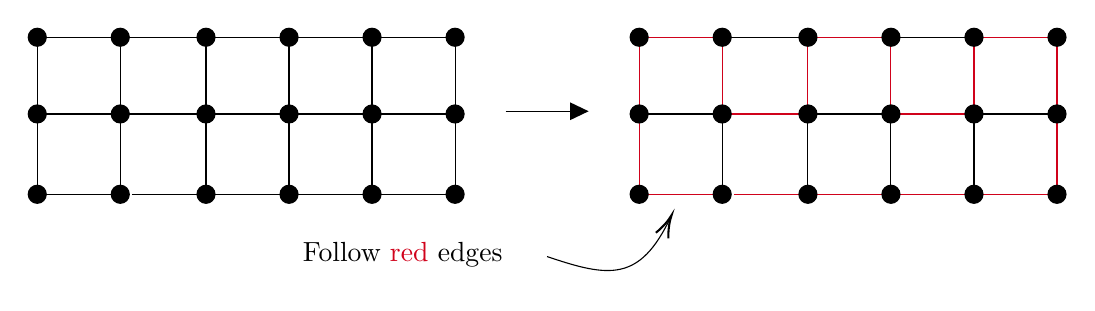
\begin{tikzpicture}[x=0.75pt,y=0.75pt,yscale=-1,xscale=1]
%uncomment if require: \path (0,244); %set diagram left start at 0, and has height of 244

%Straight Lines [id:da5413874495577164] 
\draw [color={rgb, 255:red, 0; green, 0; blue, 0 }  ,draw opacity=1 ]   (245.65,101.31) -- (285.65,101.31) ;
%Straight Lines [id:da9874152444454295] 
\draw [color={rgb, 255:red, 0; green, 0; blue, 0 }  ,draw opacity=1 ]   (88.69,140) -- (128.69,140) ;
%Straight Lines [id:da3494294488361126] 
\draw [color={rgb, 255:red, 0; green, 0; blue, 0 }  ,draw opacity=1 ]   (130,140) -- (170,140) ;
%Straight Lines [id:da2209087692914995] 
\draw [color={rgb, 255:red, 0; green, 0; blue, 0 }  ,draw opacity=1 ]   (165.65,140) -- (205.65,140) ;
%Straight Lines [id:da11559169856379725] 
\draw [color={rgb, 255:red, 0; green, 0; blue, 0 }  ,draw opacity=1 ]   (205.65,140) -- (245.65,140) ;
%Straight Lines [id:da8060090969889057] 
\draw [color={rgb, 255:red, 0; green, 0; blue, 0 }  ,draw opacity=1 ]   (245.65,140) -- (285.65,140) ;
%Straight Lines [id:da47260855483975794] 
\draw [color={rgb, 255:red, 0; green, 0; blue, 0 }  ,draw opacity=1 ]   (84.35,101.31) -- (124.35,101.31) ;
%Straight Lines [id:da850535632915091] 
\draw [color={rgb, 255:red, 0; green, 0; blue, 0 }  ,draw opacity=1 ]   (125.65,101.31) -- (165.65,101.31) ;
%Straight Lines [id:da2822613965433579] 
\draw [color={rgb, 255:red, 0; green, 0; blue, 0 }  ,draw opacity=1 ]   (170,101.31) -- (210,101.31) ;
%Straight Lines [id:da38518664257644164] 
\draw [color={rgb, 255:red, 0; green, 0; blue, 0 }  ,draw opacity=1 ]   (210,101.31) -- (250,101.31) ;
%Straight Lines [id:da41590743048687995] 
\draw [color={rgb, 255:red, 0; green, 0; blue, 0 }  ,draw opacity=1 ]   (84.35,101.31) -- (84.35,140) ;
%Straight Lines [id:da8363839204406239] 
\draw [color={rgb, 255:red, 0; green, 0; blue, 0 }  ,draw opacity=1 ]   (124.35,101.31) -- (124.35,140) ;
%Straight Lines [id:da968438967055855] 
\draw [color={rgb, 255:red, 0; green, 0; blue, 0 }  ,draw opacity=1 ]   (165.65,101.31) -- (165.65,140) ;
%Straight Lines [id:da030419789711054968] 
\draw [color={rgb, 255:red, 0; green, 0; blue, 0 }  ,draw opacity=1 ]   (205.65,101.31) -- (205.65,140) ;
%Straight Lines [id:da7397140673611776] 
\draw [color={rgb, 255:red, 0; green, 0; blue, 0 }  ,draw opacity=1 ]   (245.65,101.31) -- (245.65,140) ;
%Straight Lines [id:da3851119349563392] 
\draw [color={rgb, 255:red, 0; green, 0; blue, 0 }  ,draw opacity=1 ]   (285.65,101.31) -- (285.65,140) ;
%Straight Lines [id:da7318652436531278] 
\draw [color={rgb, 255:red, 0; green, 0; blue, 0 }  ,draw opacity=1 ]   (84.35,64.35) -- (124.35,64.35) ;
%Straight Lines [id:da4146357675888881] 
\draw [color={rgb, 255:red, 0; green, 0; blue, 0 }  ,draw opacity=1 ]   (125.65,64.35) -- (165.65,64.35) ;
%Straight Lines [id:da995555057949625] 
\draw [color={rgb, 255:red, 0; green, 0; blue, 0 }  ,draw opacity=1 ]   (165.65,64.35) -- (205.65,64.35) ;
%Straight Lines [id:da5395990910406703] 
\draw [color={rgb, 255:red, 0; green, 0; blue, 0 }  ,draw opacity=1 ]   (205.65,64.35) -- (245.65,64.35) ;
%Straight Lines [id:da6714249633605167] 
\draw [color={rgb, 255:red, 0; green, 0; blue, 0 }  ,draw opacity=1 ]   (245.65,64.35) -- (285.65,64.35) ;
%Straight Lines [id:da527686399903683] 
\draw [color={rgb, 255:red, 0; green, 0; blue, 0 }  ,draw opacity=1 ]   (84.35,64.35) -- (84.35,103.04) ;
%Straight Lines [id:da9657398084642235] 
\draw [color={rgb, 255:red, 0; green, 0; blue, 0 }  ,draw opacity=1 ]   (124.35,64.35) -- (124.35,103.04) ;
%Straight Lines [id:da08432349246427195] 
\draw [color={rgb, 255:red, 0; green, 0; blue, 0 }  ,draw opacity=1 ]   (165.65,64.35) -- (165.65,103.04) ;
%Straight Lines [id:da2856031245812556] 
\draw [color={rgb, 255:red, 0; green, 0; blue, 0 }  ,draw opacity=1 ]   (205.65,64.35) -- (205.65,103.04) ;
%Straight Lines [id:da9120675257949319] 
\draw [color={rgb, 255:red, 0; green, 0; blue, 0 }  ,draw opacity=1 ]   (245.65,64.35) -- (245.65,103.04) ;
%Straight Lines [id:da7750905610216346] 
\draw [color={rgb, 255:red, 0; green, 0; blue, 0 }  ,draw opacity=1 ]   (285.65,64.35) -- (285.65,103.04) ;
%Shape: Ellipse [id:dp00017919643503128135] 
\draw  [color={rgb, 255:red, 0; green, 0; blue, 0 }  ,draw opacity=1 ][fill={rgb, 255:red, 0; green, 0; blue, 0 }  ,fill opacity=1 ] (80,140) .. controls (80,137.6) and (81.95,135.65) .. (84.35,135.65) .. controls (86.74,135.65) and (88.69,137.6) .. (88.69,140) .. controls (88.69,142.4) and (86.74,144.35) .. (84.35,144.35) .. controls (81.95,144.35) and (80,142.4) .. (80,140) -- cycle ;
%Shape: Ellipse [id:dp7323096112154867] 
\draw  [color={rgb, 255:red, 0; green, 0; blue, 0 }  ,draw opacity=1 ][fill={rgb, 255:red, 0; green, 0; blue, 0 }  ,fill opacity=1 ] (120,140) .. controls (120,137.6) and (121.95,135.65) .. (124.35,135.65) .. controls (126.74,135.65) and (128.69,137.6) .. (128.69,140) .. controls (128.69,142.4) and (126.74,144.35) .. (124.35,144.35) .. controls (121.95,144.35) and (120,142.4) .. (120,140) -- cycle ;
%Shape: Ellipse [id:dp9239673563554562] 
\draw  [color={rgb, 255:red, 0; green, 0; blue, 0 }  ,draw opacity=1 ][fill={rgb, 255:red, 0; green, 0; blue, 0 }  ,fill opacity=1 ] (201.31,140) .. controls (201.31,137.6) and (203.26,135.65) .. (205.65,135.65) .. controls (208.05,135.65) and (210,137.6) .. (210,140) .. controls (210,142.4) and (208.05,144.35) .. (205.65,144.35) .. controls (203.26,144.35) and (201.31,142.4) .. (201.31,140) -- cycle ;
%Shape: Ellipse [id:dp4361793093757017] 
\draw  [color={rgb, 255:red, 0; green, 0; blue, 0 }  ,draw opacity=1 ][fill={rgb, 255:red, 0; green, 0; blue, 0 }  ,fill opacity=1 ] (241.31,140) .. controls (241.31,137.6) and (243.26,135.65) .. (245.65,135.65) .. controls (248.05,135.65) and (250,137.6) .. (250,140) .. controls (250,142.4) and (248.05,144.35) .. (245.65,144.35) .. controls (243.26,144.35) and (241.31,142.4) .. (241.31,140) -- cycle ;
%Shape: Ellipse [id:dp4382800131428902] 
\draw  [color={rgb, 255:red, 0; green, 0; blue, 0 }  ,draw opacity=1 ][fill={rgb, 255:red, 0; green, 0; blue, 0 }  ,fill opacity=1 ] (120,101.31) .. controls (120,98.91) and (121.95,96.96) .. (124.35,96.96) .. controls (126.74,96.96) and (128.69,98.91) .. (128.69,101.31) .. controls (128.69,103.71) and (126.74,105.65) .. (124.35,105.65) .. controls (121.95,105.65) and (120,103.71) .. (120,101.31) -- cycle ;
%Shape: Ellipse [id:dp2615142437261371] 
\draw  [color={rgb, 255:red, 0; green, 0; blue, 0 }  ,draw opacity=1 ][fill={rgb, 255:red, 0; green, 0; blue, 0 }  ,fill opacity=1 ] (201.31,101.31) .. controls (201.31,98.91) and (203.26,96.96) .. (205.65,96.96) .. controls (208.05,96.96) and (210,98.91) .. (210,101.31) .. controls (210,103.71) and (208.05,105.65) .. (205.65,105.65) .. controls (203.26,105.65) and (201.31,103.71) .. (201.31,101.31) -- cycle ;
%Shape: Ellipse [id:dp9787090224243711] 
\draw  [color={rgb, 255:red, 0; green, 0; blue, 0 }  ,draw opacity=1 ][fill={rgb, 255:red, 0; green, 0; blue, 0 }  ,fill opacity=1 ] (241.31,101.31) .. controls (241.31,98.91) and (243.26,96.96) .. (245.65,96.96) .. controls (248.05,96.96) and (250,98.91) .. (250,101.31) .. controls (250,103.71) and (248.05,105.65) .. (245.65,105.65) .. controls (243.26,105.65) and (241.31,103.71) .. (241.31,101.31) -- cycle ;
%Shape: Ellipse [id:dp6904308047172582] 
\draw  [color={rgb, 255:red, 0; green, 0; blue, 0 }  ,draw opacity=1 ][fill={rgb, 255:red, 0; green, 0; blue, 0 }  ,fill opacity=1 ] (281.31,101.31) .. controls (281.31,98.91) and (283.26,96.96) .. (285.65,96.96) .. controls (288.05,96.96) and (290,98.91) .. (290,101.31) .. controls (290,103.71) and (288.05,105.65) .. (285.65,105.65) .. controls (283.26,105.65) and (281.31,103.71) .. (281.31,101.31) -- cycle ;
%Shape: Ellipse [id:dp01148886914018099] 
\draw  [color={rgb, 255:red, 0; green, 0; blue, 0 }  ,draw opacity=1 ][fill={rgb, 255:red, 0; green, 0; blue, 0 }  ,fill opacity=1 ] (80,101.31) .. controls (80,98.91) and (81.95,96.96) .. (84.35,96.96) .. controls (86.74,96.96) and (88.69,98.91) .. (88.69,101.31) .. controls (88.69,103.71) and (86.74,105.65) .. (84.35,105.65) .. controls (81.95,105.65) and (80,103.71) .. (80,101.31) -- cycle ;
%Shape: Ellipse [id:dp6016324397088084] 
\draw  [color={rgb, 255:red, 0; green, 0; blue, 0 }  ,draw opacity=1 ][fill={rgb, 255:red, 0; green, 0; blue, 0 }  ,fill opacity=1 ] (281.31,140) .. controls (281.31,137.6) and (283.26,135.65) .. (285.65,135.65) .. controls (288.05,135.65) and (290,137.6) .. (290,140) .. controls (290,142.4) and (288.05,144.35) .. (285.65,144.35) .. controls (283.26,144.35) and (281.31,142.4) .. (281.31,140) -- cycle ;
%Shape: Ellipse [id:dp6832469309236383] 
\draw  [color={rgb, 255:red, 0; green, 0; blue, 0 }  ,draw opacity=1 ][fill={rgb, 255:red, 0; green, 0; blue, 0 }  ,fill opacity=1 ] (161.31,140) .. controls (161.31,137.6) and (163.26,135.65) .. (165.65,135.65) .. controls (168.05,135.65) and (170,137.6) .. (170,140) .. controls (170,142.4) and (168.05,144.35) .. (165.65,144.35) .. controls (163.26,144.35) and (161.31,142.4) .. (161.31,140) -- cycle ;
%Shape: Ellipse [id:dp9427473506609012] 
\draw  [color={rgb, 255:red, 0; green, 0; blue, 0 }  ,draw opacity=1 ][fill={rgb, 255:red, 0; green, 0; blue, 0 }  ,fill opacity=1 ] (161.31,101.31) .. controls (161.31,98.91) and (163.26,96.96) .. (165.65,96.96) .. controls (168.05,96.96) and (170,98.91) .. (170,101.31) .. controls (170,103.71) and (168.05,105.65) .. (165.65,105.65) .. controls (163.26,105.65) and (161.31,103.71) .. (161.31,101.31) -- cycle ;
%Shape: Ellipse [id:dp05916149502624202] 
\draw  [color={rgb, 255:red, 0; green, 0; blue, 0 }  ,draw opacity=1 ][fill={rgb, 255:red, 0; green, 0; blue, 0 }  ,fill opacity=1 ] (120,64.35) .. controls (120,61.95) and (121.95,60) .. (124.35,60) .. controls (126.74,60) and (128.69,61.95) .. (128.69,64.35) .. controls (128.69,66.74) and (126.74,68.69) .. (124.35,68.69) .. controls (121.95,68.69) and (120,66.74) .. (120,64.35) -- cycle ;
%Shape: Ellipse [id:dp14517159860717266] 
\draw  [color={rgb, 255:red, 0; green, 0; blue, 0 }  ,draw opacity=1 ][fill={rgb, 255:red, 0; green, 0; blue, 0 }  ,fill opacity=1 ] (201.31,64.35) .. controls (201.31,61.95) and (203.26,60) .. (205.65,60) .. controls (208.05,60) and (210,61.95) .. (210,64.35) .. controls (210,66.74) and (208.05,68.69) .. (205.65,68.69) .. controls (203.26,68.69) and (201.31,66.74) .. (201.31,64.35) -- cycle ;
%Shape: Ellipse [id:dp43118171718750553] 
\draw  [color={rgb, 255:red, 0; green, 0; blue, 0 }  ,draw opacity=1 ][fill={rgb, 255:red, 0; green, 0; blue, 0 }  ,fill opacity=1 ] (241.31,64.35) .. controls (241.31,61.95) and (243.26,60) .. (245.65,60) .. controls (248.05,60) and (250,61.95) .. (250,64.35) .. controls (250,66.74) and (248.05,68.69) .. (245.65,68.69) .. controls (243.26,68.69) and (241.31,66.74) .. (241.31,64.35) -- cycle ;
%Shape: Ellipse [id:dp5781936928760221] 
\draw  [color={rgb, 255:red, 0; green, 0; blue, 0 }  ,draw opacity=1 ][fill={rgb, 255:red, 0; green, 0; blue, 0 }  ,fill opacity=1 ] (281.31,64.35) .. controls (281.31,61.95) and (283.26,60) .. (285.65,60) .. controls (288.05,60) and (290,61.95) .. (290,64.35) .. controls (290,66.74) and (288.05,68.69) .. (285.65,68.69) .. controls (283.26,68.69) and (281.31,66.74) .. (281.31,64.35) -- cycle ;
%Shape: Ellipse [id:dp5571453768202594] 
\draw  [color={rgb, 255:red, 0; green, 0; blue, 0 }  ,draw opacity=1 ][fill={rgb, 255:red, 0; green, 0; blue, 0 }  ,fill opacity=1 ] (80,64.35) .. controls (80,61.95) and (81.95,60) .. (84.35,60) .. controls (86.74,60) and (88.69,61.95) .. (88.69,64.35) .. controls (88.69,66.74) and (86.74,68.69) .. (84.35,68.69) .. controls (81.95,68.69) and (80,66.74) .. (80,64.35) -- cycle ;
%Shape: Ellipse [id:dp7117974042275724] 
\draw  [color={rgb, 255:red, 0; green, 0; blue, 0 }  ,draw opacity=1 ][fill={rgb, 255:red, 0; green, 0; blue, 0 }  ,fill opacity=1 ] (161.31,64.35) .. controls (161.31,61.95) and (163.26,60) .. (165.65,60) .. controls (168.05,60) and (170,61.95) .. (170,64.35) .. controls (170,66.74) and (168.05,68.69) .. (165.65,68.69) .. controls (163.26,68.69) and (161.31,66.74) .. (161.31,64.35) -- cycle ;
%Straight Lines [id:da16809371572584741] 
\draw [color={rgb, 255:red, 0; green, 0; blue, 0 }  ,draw opacity=1 ]   (535.65,101.31) -- (575.65,101.31) ;
%Straight Lines [id:da05573221606436096] 
\draw [color={rgb, 255:red, 208; green, 2; blue, 27 }  ,draw opacity=1 ]   (378.69,140) -- (418.69,140) ;
%Straight Lines [id:da03737210575480443] 
\draw [color={rgb, 255:red, 208; green, 2; blue, 27 }  ,draw opacity=1 ]   (420,140) -- (460,140) ;
%Straight Lines [id:da7676400488241927] 
\draw [color={rgb, 255:red, 208; green, 2; blue, 27 }  ,draw opacity=1 ]   (455.65,140) -- (495.65,140) ;
%Straight Lines [id:da03940349732277404] 
\draw [color={rgb, 255:red, 208; green, 2; blue, 27 }  ,draw opacity=1 ]   (495.65,140) -- (535.65,140) ;
%Straight Lines [id:da576367351740554] 
\draw [color={rgb, 255:red, 208; green, 2; blue, 27 }  ,draw opacity=1 ]   (535.65,140) -- (575.65,140) ;
%Straight Lines [id:da06490880028604562] 
\draw [color={rgb, 255:red, 0; green, 0; blue, 0 }  ,draw opacity=1 ]   (374.35,101.31) -- (414.35,101.31) ;
%Straight Lines [id:da045149746063365415] 
\draw [color={rgb, 255:red, 208; green, 2; blue, 27 }  ,draw opacity=1 ]   (415.65,101.31) -- (455.65,101.31) ;
%Straight Lines [id:da34018177569870134] 
\draw [color={rgb, 255:red, 0; green, 0; blue, 0 }  ,draw opacity=1 ]   (460,101.31) -- (500,101.31) ;
%Straight Lines [id:da08880678231409167] 
\draw [color={rgb, 255:red, 208; green, 2; blue, 27 }  ,draw opacity=1 ]   (500,101.31) -- (540,101.31) ;
%Straight Lines [id:da18563266405210777] 
\draw [color={rgb, 255:red, 208; green, 2; blue, 27 }  ,draw opacity=1 ]   (374.35,101.31) -- (374.35,140) ;
%Straight Lines [id:da7651278246039379] 
\draw [color={rgb, 255:red, 0; green, 0; blue, 0 }  ,draw opacity=1 ]   (414.35,101.31) -- (414.35,140) ;
%Straight Lines [id:da17782756907323927] 
\draw [color={rgb, 255:red, 0; green, 0; blue, 0 }  ,draw opacity=1 ]   (455.65,101.31) -- (455.65,140) ;
%Straight Lines [id:da3577235251753559] 
\draw [color={rgb, 255:red, 0; green, 0; blue, 0 }  ,draw opacity=1 ]   (495.65,101.31) -- (495.65,140) ;
%Straight Lines [id:da9419330234648975] 
\draw [color={rgb, 255:red, 0; green, 0; blue, 0 }  ,draw opacity=1 ]   (535.65,101.31) -- (535.65,140) ;
%Straight Lines [id:da2920393051152824] 
\draw [color={rgb, 255:red, 208; green, 2; blue, 27 }  ,draw opacity=1 ]   (575.65,101.31) -- (575.65,140) ;
%Straight Lines [id:da10497647037340596] 
\draw [color={rgb, 255:red, 208; green, 2; blue, 27 }  ,draw opacity=1 ]   (374.35,64.35) -- (414.35,64.35) ;
%Straight Lines [id:da6456772624658789] 
\draw [color={rgb, 255:red, 0; green, 0; blue, 0 }  ,draw opacity=1 ]   (415.65,64.35) -- (455.65,64.35) ;
%Straight Lines [id:da45186789920067894] 
\draw [color={rgb, 255:red, 208; green, 2; blue, 27 }  ,draw opacity=1 ]   (455.65,64.35) -- (495.65,64.35) ;
%Straight Lines [id:da38014667986538] 
\draw [color={rgb, 255:red, 0; green, 0; blue, 0 }  ,draw opacity=1 ]   (495.65,64.35) -- (535.65,64.35) ;
%Straight Lines [id:da1004194534581746] 
\draw [color={rgb, 255:red, 208; green, 2; blue, 27 }  ,draw opacity=1 ]   (535.65,64.35) -- (575.65,64.35) ;
%Straight Lines [id:da5553926966424764] 
\draw [color={rgb, 255:red, 208; green, 2; blue, 27 }  ,draw opacity=1 ]   (374.35,64.35) -- (374.35,103.04) ;
%Straight Lines [id:da3988650850842287] 
\draw [color={rgb, 255:red, 208; green, 2; blue, 27 }  ,draw opacity=1 ]   (414.35,64.35) -- (414.35,103.04) ;
%Straight Lines [id:da9827316941379681] 
\draw [color={rgb, 255:red, 208; green, 2; blue, 27 }  ,draw opacity=1 ]   (455.65,64.35) -- (455.65,103.04) ;
%Straight Lines [id:da08936781169793728] 
\draw [color={rgb, 255:red, 208; green, 2; blue, 27 }  ,draw opacity=1 ]   (495.65,64.35) -- (495.65,103.04) ;
%Straight Lines [id:da14847286270741156] 
\draw [color={rgb, 255:red, 208; green, 2; blue, 27 }  ,draw opacity=1 ]   (535.65,64.35) -- (535.65,103.04) ;
%Straight Lines [id:da0659278348522806] 
\draw [color={rgb, 255:red, 208; green, 2; blue, 27 }  ,draw opacity=1 ]   (575.65,64.35) -- (575.65,103.04) ;
%Shape: Ellipse [id:dp8053501082977472] 
\draw  [color={rgb, 255:red, 0; green, 0; blue, 0 }  ,draw opacity=1 ][fill={rgb, 255:red, 0; green, 0; blue, 0 }  ,fill opacity=1 ] (370,140) .. controls (370,137.6) and (371.95,135.65) .. (374.35,135.65) .. controls (376.74,135.65) and (378.69,137.6) .. (378.69,140) .. controls (378.69,142.4) and (376.74,144.35) .. (374.35,144.35) .. controls (371.95,144.35) and (370,142.4) .. (370,140) -- cycle ;
%Shape: Ellipse [id:dp7319908626805294] 
\draw  [color={rgb, 255:red, 0; green, 0; blue, 0 }  ,draw opacity=1 ][fill={rgb, 255:red, 0; green, 0; blue, 0 }  ,fill opacity=1 ] (410,140) .. controls (410,137.6) and (411.95,135.65) .. (414.35,135.65) .. controls (416.74,135.65) and (418.69,137.6) .. (418.69,140) .. controls (418.69,142.4) and (416.74,144.35) .. (414.35,144.35) .. controls (411.95,144.35) and (410,142.4) .. (410,140) -- cycle ;
%Shape: Ellipse [id:dp5287317745131638] 
\draw  [color={rgb, 255:red, 0; green, 0; blue, 0 }  ,draw opacity=1 ][fill={rgb, 255:red, 0; green, 0; blue, 0 }  ,fill opacity=1 ] (491.31,140) .. controls (491.31,137.6) and (493.26,135.65) .. (495.65,135.65) .. controls (498.05,135.65) and (500,137.6) .. (500,140) .. controls (500,142.4) and (498.05,144.35) .. (495.65,144.35) .. controls (493.26,144.35) and (491.31,142.4) .. (491.31,140) -- cycle ;
%Shape: Ellipse [id:dp45081675432140134] 
\draw  [color={rgb, 255:red, 0; green, 0; blue, 0 }  ,draw opacity=1 ][fill={rgb, 255:red, 0; green, 0; blue, 0 }  ,fill opacity=1 ] (531.31,140) .. controls (531.31,137.6) and (533.26,135.65) .. (535.65,135.65) .. controls (538.05,135.65) and (540,137.6) .. (540,140) .. controls (540,142.4) and (538.05,144.35) .. (535.65,144.35) .. controls (533.26,144.35) and (531.31,142.4) .. (531.31,140) -- cycle ;
%Shape: Ellipse [id:dp5201577383844709] 
\draw  [color={rgb, 255:red, 0; green, 0; blue, 0 }  ,draw opacity=1 ][fill={rgb, 255:red, 0; green, 0; blue, 0 }  ,fill opacity=1 ] (410,101.31) .. controls (410,98.91) and (411.95,96.96) .. (414.35,96.96) .. controls (416.74,96.96) and (418.69,98.91) .. (418.69,101.31) .. controls (418.69,103.71) and (416.74,105.65) .. (414.35,105.65) .. controls (411.95,105.65) and (410,103.71) .. (410,101.31) -- cycle ;
%Shape: Ellipse [id:dp09632913642872287] 
\draw  [color={rgb, 255:red, 0; green, 0; blue, 0 }  ,draw opacity=1 ][fill={rgb, 255:red, 0; green, 0; blue, 0 }  ,fill opacity=1 ] (491.31,101.31) .. controls (491.31,98.91) and (493.26,96.96) .. (495.65,96.96) .. controls (498.05,96.96) and (500,98.91) .. (500,101.31) .. controls (500,103.71) and (498.05,105.65) .. (495.65,105.65) .. controls (493.26,105.65) and (491.31,103.71) .. (491.31,101.31) -- cycle ;
%Shape: Ellipse [id:dp39851973159176224] 
\draw  [color={rgb, 255:red, 0; green, 0; blue, 0 }  ,draw opacity=1 ][fill={rgb, 255:red, 0; green, 0; blue, 0 }  ,fill opacity=1 ] (531.31,101.31) .. controls (531.31,98.91) and (533.26,96.96) .. (535.65,96.96) .. controls (538.05,96.96) and (540,98.91) .. (540,101.31) .. controls (540,103.71) and (538.05,105.65) .. (535.65,105.65) .. controls (533.26,105.65) and (531.31,103.71) .. (531.31,101.31) -- cycle ;
%Shape: Ellipse [id:dp5161284838385125] 
\draw  [color={rgb, 255:red, 0; green, 0; blue, 0 }  ,draw opacity=1 ][fill={rgb, 255:red, 0; green, 0; blue, 0 }  ,fill opacity=1 ] (571.31,101.31) .. controls (571.31,98.91) and (573.26,96.96) .. (575.65,96.96) .. controls (578.05,96.96) and (580,98.91) .. (580,101.31) .. controls (580,103.71) and (578.05,105.65) .. (575.65,105.65) .. controls (573.26,105.65) and (571.31,103.71) .. (571.31,101.31) -- cycle ;
%Shape: Ellipse [id:dp30647627059387705] 
\draw  [color={rgb, 255:red, 0; green, 0; blue, 0 }  ,draw opacity=1 ][fill={rgb, 255:red, 0; green, 0; blue, 0 }  ,fill opacity=1 ] (370,101.31) .. controls (370,98.91) and (371.95,96.96) .. (374.35,96.96) .. controls (376.74,96.96) and (378.69,98.91) .. (378.69,101.31) .. controls (378.69,103.71) and (376.74,105.65) .. (374.35,105.65) .. controls (371.95,105.65) and (370,103.71) .. (370,101.31) -- cycle ;
%Shape: Ellipse [id:dp6405526199734636] 
\draw  [color={rgb, 255:red, 0; green, 0; blue, 0 }  ,draw opacity=1 ][fill={rgb, 255:red, 0; green, 0; blue, 0 }  ,fill opacity=1 ] (571.31,140) .. controls (571.31,137.6) and (573.26,135.65) .. (575.65,135.65) .. controls (578.05,135.65) and (580,137.6) .. (580,140) .. controls (580,142.4) and (578.05,144.35) .. (575.65,144.35) .. controls (573.26,144.35) and (571.31,142.4) .. (571.31,140) -- cycle ;
%Shape: Ellipse [id:dp04010507849346068] 
\draw  [color={rgb, 255:red, 0; green, 0; blue, 0 }  ,draw opacity=1 ][fill={rgb, 255:red, 0; green, 0; blue, 0 }  ,fill opacity=1 ] (451.31,140) .. controls (451.31,137.6) and (453.26,135.65) .. (455.65,135.65) .. controls (458.05,135.65) and (460,137.6) .. (460,140) .. controls (460,142.4) and (458.05,144.35) .. (455.65,144.35) .. controls (453.26,144.35) and (451.31,142.4) .. (451.31,140) -- cycle ;
%Shape: Ellipse [id:dp8275412766651555] 
\draw  [color={rgb, 255:red, 0; green, 0; blue, 0 }  ,draw opacity=1 ][fill={rgb, 255:red, 0; green, 0; blue, 0 }  ,fill opacity=1 ] (451.31,101.31) .. controls (451.31,98.91) and (453.26,96.96) .. (455.65,96.96) .. controls (458.05,96.96) and (460,98.91) .. (460,101.31) .. controls (460,103.71) and (458.05,105.65) .. (455.65,105.65) .. controls (453.26,105.65) and (451.31,103.71) .. (451.31,101.31) -- cycle ;
%Shape: Ellipse [id:dp5635000123159486] 
\draw  [color={rgb, 255:red, 0; green, 0; blue, 0 }  ,draw opacity=1 ][fill={rgb, 255:red, 0; green, 0; blue, 0 }  ,fill opacity=1 ] (410,64.35) .. controls (410,61.95) and (411.95,60) .. (414.35,60) .. controls (416.74,60) and (418.69,61.95) .. (418.69,64.35) .. controls (418.69,66.74) and (416.74,68.69) .. (414.35,68.69) .. controls (411.95,68.69) and (410,66.74) .. (410,64.35) -- cycle ;
%Shape: Ellipse [id:dp679536524297763] 
\draw  [color={rgb, 255:red, 0; green, 0; blue, 0 }  ,draw opacity=1 ][fill={rgb, 255:red, 0; green, 0; blue, 0 }  ,fill opacity=1 ] (491.31,64.35) .. controls (491.31,61.95) and (493.26,60) .. (495.65,60) .. controls (498.05,60) and (500,61.95) .. (500,64.35) .. controls (500,66.74) and (498.05,68.69) .. (495.65,68.69) .. controls (493.26,68.69) and (491.31,66.74) .. (491.31,64.35) -- cycle ;
%Shape: Ellipse [id:dp6611131255285665] 
\draw  [color={rgb, 255:red, 0; green, 0; blue, 0 }  ,draw opacity=1 ][fill={rgb, 255:red, 0; green, 0; blue, 0 }  ,fill opacity=1 ] (531.31,64.35) .. controls (531.31,61.95) and (533.26,60) .. (535.65,60) .. controls (538.05,60) and (540,61.95) .. (540,64.35) .. controls (540,66.74) and (538.05,68.69) .. (535.65,68.69) .. controls (533.26,68.69) and (531.31,66.74) .. (531.31,64.35) -- cycle ;
%Shape: Ellipse [id:dp5010822966083567] 
\draw  [color={rgb, 255:red, 0; green, 0; blue, 0 }  ,draw opacity=1 ][fill={rgb, 255:red, 0; green, 0; blue, 0 }  ,fill opacity=1 ] (571.31,64.35) .. controls (571.31,61.95) and (573.26,60) .. (575.65,60) .. controls (578.05,60) and (580,61.95) .. (580,64.35) .. controls (580,66.74) and (578.05,68.69) .. (575.65,68.69) .. controls (573.26,68.69) and (571.31,66.74) .. (571.31,64.35) -- cycle ;
%Shape: Ellipse [id:dp04331764362306778] 
\draw  [color={rgb, 255:red, 0; green, 0; blue, 0 }  ,draw opacity=1 ][fill={rgb, 255:red, 0; green, 0; blue, 0 }  ,fill opacity=1 ] (370,64.35) .. controls (370,61.95) and (371.95,60) .. (374.35,60) .. controls (376.74,60) and (378.69,61.95) .. (378.69,64.35) .. controls (378.69,66.74) and (376.74,68.69) .. (374.35,68.69) .. controls (371.95,68.69) and (370,66.74) .. (370,64.35) -- cycle ;
%Shape: Ellipse [id:dp4903805130487763] 
\draw  [color={rgb, 255:red, 0; green, 0; blue, 0 }  ,draw opacity=1 ][fill={rgb, 255:red, 0; green, 0; blue, 0 }  ,fill opacity=1 ] (451.31,64.35) .. controls (451.31,61.95) and (453.26,60) .. (455.65,60) .. controls (458.05,60) and (460,61.95) .. (460,64.35) .. controls (460,66.74) and (458.05,68.69) .. (455.65,68.69) .. controls (453.26,68.69) and (451.31,66.74) .. (451.31,64.35) -- cycle ;
%Straight Lines [id:da05894247913970363] 
\draw    (310,100) -- (347,100) ;
\draw [shift={(350,100)}, rotate = 180] [fill={rgb, 255:red, 0; green, 0; blue, 0 }  ][line width=0.08]  [draw opacity=0] (8.93,-4.29) -- (0,0) -- (8.93,4.29) -- cycle    ;
%Curve Lines [id:da04409052844433903] 
\draw    (330,170) .. controls (359.88,180.18) and (374.56,182.27) .. (389.33,151.43) ;
\draw [shift={(390,150)}, rotate = 474.89] [color={rgb, 255:red, 0; green, 0; blue, 0 }  ][line width=0.75]    (10.93,-3.29) .. controls (6.95,-1.4) and (3.31,-0.3) .. (0,0) .. controls (3.31,0.3) and (6.95,1.4) .. (10.93,3.29)   ;

% Text Node
\draw (211,162) node [anchor=north west][inner sep=0.75pt]   [align=left] {Follow \textcolor[rgb]{0.82,0.01,0.11}{red} edges};


\end{tikzpicture}

\end{center}


Our first question might be `is there an iff type condition for Hamiltonian cycles', and so far there is no such property known. However there are some results that give us information about whether a graph is Hamiltonian.

\begin{theorem}[Dirac's Theorem]
	Let $G$ be a graph with $n\geq 3$ such that $\delta(G) \geq n/2$. Then $G$ contains a Hamiltonian cycle.
\end{theorem}
\begin{proof}
	For a contradiction, assume that $G$ is a counterexample to the theorem.
	Note that $G$ is connected, since $x \not \sim y$ then $N(x), N(y) \subset V \backslash\{x, y\}$ and $|N(x)|, |N(y)| \geq \frac{n}{2}$, and thus $N(x) \cap N(y) \neq \emptyset$, and thus $d(x, y) \leq 2$.

	Let $x_1, \dots, x_\ell$ be the longest path in $G$. Note that $x_1, \dots, x_\ell$ does not form a cycle, as otherwise if $\ell = n$, then we have a contradiction, and if $\ell < n$ then there exists $y \not \in \{x_1, \dots, x_\ell\}$ that is $y \sim x_i$. Thus we can find a longer path (which is also a contradiction).

	Now if there exists $i \in \{1, \dots, \ell - 1\}$ so that $x_i \sim x_\ell$ and $x_{i + 1} \sim x_1$, then the vertices $x_1, \dots, x_\ell$ form a cycle. This contradicts the above.

	Define
	$$
	N^+(x_\ell) = \{x_i \mid x_{i - 1} \in N(X_l), 2 \leq i \leq \ell\}.
	$$
	We have $N^+(x_\ell) \cap N(x_1) = \empty$, but this is impossible since $|N^+(x_\ell)| \geq n/2$, $|N(x_1)| \geq n/2$, and $N^+(x_\ell), N(x_1) \subseteq \{x_2, \dots, x_\ell\}$. Thus we have a contradiction.
\end{proof}

\begin{remark}
	We never \emph{really} used this $\delta(G) \geq n/2$ condition fully. It suffices to have $d(x) + d(y) \geq n$ for $x \not \sim y$.
\end{remark}

We can use this same argument to prove a more general result about paths.

\begin{proposition}\label{prop:used-here}
	Let $G$ be a connected graph. Let $k < n$ and assume $\delta(G) \geq k/2$. Then $G \geq P_{k + 1}$.
\end{proposition}
\begin{proof}[Proof Sketch]
	Similar to Dirac's theorem. Choose a longest path $x_1, \dots, x_\ell$ in $G$. They don't form a cycle, and then we can force a configuration like $x_1 \sum x_{i + 1}$, $x_{\ell} \sum x_i$ by using the minimum degree condition.
\end{proof}

We may wonder in the above if it's possible to replace `path' with `cycle' in the above. The answer is, sadly, no.

A natural question is to wonder how many edges are needed to `force' a (for example) triangle.
For a Hamilton cycle, this sort of question would have been a bit strange, and a more natural question would be what is the minimum value of $\delta(G)$ to ensure that $G$ contains a Hamilton cycle.
In the next theorem, we will give a result that answers a simpler sort of question.

\begin{theorem}
	Let $G$ be a graph. If $e(G) > \frac{n}{2}(k - 1)$, then $G$ contains a path of length $k$.
\end{theorem}
\begin{proof}
	We will prove the contrapositive: If $G$ is $P_{k + 1}$ free, then $e(G) \leq \frac{n}{2}(k - 1)$.

	We will apply induction on $n$. This is true for $n = 2$.
	Then given a graph $G$ on $|G| = n \geq 3$ vertices, if $G$ is disconnected let $G_1, \dots, G_k$ be the components of $G$. Then each of these has $G_i \not \supseteq P_{k + 1}$. Then by induction we have $e(G_i) \leq \frac{n(G_i)(k - 1)}{2}$. Thus
	$$
	e(G) = \sum_{i = 1}^k e(G_i) \leq \sum \frac{n(G_i)(k - 1)}{2} = \left(\frac{k - 1}{2}\right)n,
	$$
	and we are done.

	Now if there is a vertex $v$ with $d(v) \leq \frac{k - 1}{2}$, then consider $G - v$. Then $e(G - v) = e(G) - d(v)$, and also $G - v$ does not contain $P_{k + 1}$. Thus $e(G - v) \leq \frac{n - 1}{2}(k - 1)$. So
	$$
	e(G) = e(G - v) + d(v) \leq \frac{n - 1}{2}(k - 1) + \frac{k -1}{2} \leq \frac{n}{2}(k - 1).
	$$
	Thus we can assume $G$ is connected and $d(v)  \geq \frac{k}{2}$.
	We we can apply \autoref{prop:used-here} to find a path of length $k$, that is, $P_{k + 1} \subseteq G$, which is a contradiction.

	[We may also assume $k < n$ for if $k = n$ then $e(G) \leq \frac{k}{2}(n - 1)$, which reduces to showing $e(G) \leq \binom{n}{2}$, which is trivial].
\end{proof}

\subsection{Complete Subgraphs and Turan's Theorem}

Let's return to the question of how many edges are needed in a graph to guarantee the existence of a triangle. Later on, we will look more generally at the question of the number of edges needed to guarantee a $K_n$ subgraph.

\begin{theorem}[Mantel's Theorem]
	If $e(G) > \frac{n^2}{4}$, then $G \supset K_3$, and this is sharp.
\end{theorem}
\begin{proof}
	Given a $K_3$-free graph $G$ and $x, y \in V$ such that $x \sim y$ and $d(x) + d(y) \leq n$, and let $m = e(G)$.
	Then summing we get
	$$
	\sum_{xy \in E} d(x) + d(y) \leq mn.
	$$
	We have that this is $\sum_x \sum_y d(x) \mathbbm{1}(xy \in E) = \sum_{x \in V} (d(x))^2$.
	Now $\sum_{x \in V} d(x) = 2m$, and by Cauchy-Schwarz we have $(\sum d(x))^2 \leq n\sum d(x)^2$, and thus
	$$
	m n^2 \geq (2m)^2 \implies \frac{n^2}{4} = e(G).
	$$

	To see that this is sharp, consider the complete bipartite graph with $n$ vertices. Then this has $n^2/4$ edges, but no triangle. Thus this is sharp.
\end{proof}

The next question we are going to answer is how many edges are needed to guarantee the existence of a $K_n$ subgraph. In the previous theorem, to see that our result was sharp, we considered the complete bipartite graph on $n$ vertices. To discuss this more general question, a natural thing to look at is a generalisation of bipartite graphs.

\begin{definition}[$r$-Partite Graph]
    An \vocab{$r$-partite graph} is a graph of the form $G = (V, E)$ where the vertices are partitioned into $r$ subsets $V = V_1 \cup \cdots \cup V_r$ with $V_i \cap V_j = \emptyset$ if $i \neq j$, and $xy \not\in E$ for all $x, y \in V_i$.
\end{definition}

For example, the graph below is $3$-partite.
\begin{center}
    

\tikzset{every picture/.style={line width=0.75pt}} %set default line width to 0.75pt        

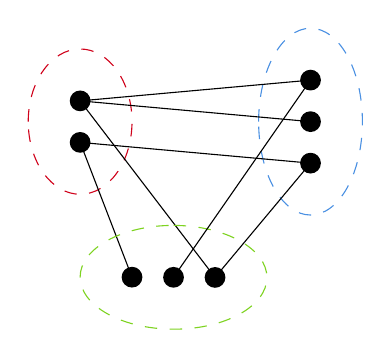
\begin{tikzpicture}[x=0.75pt,y=0.75pt,yscale=-1,xscale=1]
%uncomment if require: \path (0,273); %set diagram left start at 0, and has height of 273

%Shape: Circle [id:dp9407388701799828] 
\draw  [draw opacity=0][fill={rgb, 255:red, 0; green, 0; blue, 0 }  ,fill opacity=1 ] (320,105) .. controls (320,102.24) and (322.24,100) .. (325,100) .. controls (327.76,100) and (330,102.24) .. (330,105) .. controls (330,107.76) and (327.76,110) .. (325,110) .. controls (322.24,110) and (320,107.76) .. (320,105) -- cycle ;
%Shape: Circle [id:dp9879317160517831] 
\draw  [draw opacity=0][fill={rgb, 255:red, 0; green, 0; blue, 0 }  ,fill opacity=1 ] (320,85) .. controls (320,82.24) and (322.24,80) .. (325,80) .. controls (327.76,80) and (330,82.24) .. (330,85) .. controls (330,87.76) and (327.76,90) .. (325,90) .. controls (322.24,90) and (320,87.76) .. (320,85) -- cycle ;
%Shape: Ellipse [id:dp689919076485602] 
\draw  [color={rgb, 255:red, 208; green, 2; blue, 27 }  ,draw opacity=1 ][dash pattern={on 4.5pt off 4.5pt}] (300,95) .. controls (300,75.67) and (311.19,60) .. (325,60) .. controls (338.81,60) and (350,75.67) .. (350,95) .. controls (350,114.33) and (338.81,130) .. (325,130) .. controls (311.19,130) and (300,114.33) .. (300,95) -- cycle ;
%Shape: Circle [id:dp5065764509864156] 
\draw  [draw opacity=0][fill={rgb, 255:red, 0; green, 0; blue, 0 }  ,fill opacity=1 ] (431,115) .. controls (431,112.24) and (433.24,110) .. (436,110) .. controls (438.76,110) and (441,112.24) .. (441,115) .. controls (441,117.76) and (438.76,120) .. (436,120) .. controls (433.24,120) and (431,117.76) .. (431,115) -- cycle ;
%Shape: Circle [id:dp7870478525688073] 
\draw  [draw opacity=0][fill={rgb, 255:red, 0; green, 0; blue, 0 }  ,fill opacity=1 ] (431,95) .. controls (431,92.24) and (433.24,90) .. (436,90) .. controls (438.76,90) and (441,92.24) .. (441,95) .. controls (441,97.76) and (438.76,100) .. (436,100) .. controls (433.24,100) and (431,97.76) .. (431,95) -- cycle ;
%Shape: Circle [id:dp6489806844882018] 
\draw  [draw opacity=0][fill={rgb, 255:red, 0; green, 0; blue, 0 }  ,fill opacity=1 ] (431,75) .. controls (431,72.24) and (433.24,70) .. (436,70) .. controls (438.76,70) and (441,72.24) .. (441,75) .. controls (441,77.76) and (438.76,80) .. (436,80) .. controls (433.24,80) and (431,77.76) .. (431,75) -- cycle ;
%Shape: Ellipse [id:dp8663794047092029] 
\draw  [color={rgb, 255:red, 74; green, 144; blue, 226 }  ,draw opacity=1 ][dash pattern={on 4.5pt off 4.5pt}] (411,95) .. controls (411,70.15) and (422.19,50) .. (436,50) .. controls (449.81,50) and (461,70.15) .. (461,95) .. controls (461,119.85) and (449.81,140) .. (436,140) .. controls (422.19,140) and (411,119.85) .. (411,95) -- cycle ;
%Straight Lines [id:da751823248575425] 
\draw [color={rgb, 255:red, 0; green, 0; blue, 0 }  ,draw opacity=1 ]   (325,85) -- (436,75) ;
%Straight Lines [id:da8492860173074633] 
\draw [color={rgb, 255:red, 0; green, 0; blue, 0 }  ,draw opacity=1 ]   (325,85) -- (436,95) ;
%Straight Lines [id:da21872966548130512] 
\draw [color={rgb, 255:red, 0; green, 0; blue, 0 }  ,draw opacity=1 ]   (325,105) -- (350,169.94) ;
%Straight Lines [id:da8502794221965817] 
\draw [color={rgb, 255:red, 0; green, 0; blue, 0 }  ,draw opacity=1 ]   (325,85) -- (390,170.06) ;
%Straight Lines [id:da8613623857391655] 
\draw [color={rgb, 255:red, 0; green, 0; blue, 0 }  ,draw opacity=1 ]   (325,105) -- (436,115) ;
%Shape: Circle [id:dp2651151962113202] 
\draw  [draw opacity=0][fill={rgb, 255:red, 0; green, 0; blue, 0 }  ,fill opacity=1 ] (350.02,164.94) .. controls (352.78,164.95) and (355.01,167.19) .. (355,169.95) .. controls (354.99,172.71) and (352.75,174.95) .. (349.98,174.94) .. controls (347.22,174.93) and (344.99,172.68) .. (345,169.92) .. controls (345.01,167.16) and (347.25,164.93) .. (350.02,164.94) -- cycle ;
%Shape: Circle [id:dp02037924201064667] 
\draw  [draw opacity=0][fill={rgb, 255:red, 0; green, 0; blue, 0 }  ,fill opacity=1 ] (370.02,165) .. controls (372.78,165.01) and (375.01,167.25) .. (375,170.02) .. controls (374.99,172.78) and (372.75,175.01) .. (369.98,175) .. controls (367.22,174.99) and (364.99,172.75) .. (365,169.98) .. controls (365.01,167.22) and (367.25,164.99) .. (370.02,165) -- cycle ;
%Shape: Circle [id:dp0031436706127647707] 
\draw  [draw opacity=0][fill={rgb, 255:red, 0; green, 0; blue, 0 }  ,fill opacity=1 ] (390.02,165.06) .. controls (392.78,165.07) and (395.01,167.32) .. (395,170.08) .. controls (394.99,172.84) and (392.75,175.07) .. (389.98,175.06) .. controls (387.22,175.05) and (384.99,172.81) .. (385,170.05) .. controls (385.01,167.29) and (387.25,165.05) .. (390.02,165.06) -- cycle ;
%Shape: Ellipse [id:dp44885950986715906] 
\draw  [color={rgb, 255:red, 126; green, 211; blue, 33 }  ,draw opacity=1 ][dash pattern={on 4.5pt off 4.5pt}] (370.08,145) .. controls (394.93,145.08) and (415.04,156.33) .. (415,170.14) .. controls (414.96,183.95) and (394.77,195.08) .. (369.92,195) .. controls (345.07,194.92) and (324.96,183.67) .. (325,169.86) .. controls (325.04,156.05) and (345.23,144.92) .. (370.08,145) -- cycle ;
%Straight Lines [id:da3164601002770683] 
\draw [color={rgb, 255:red, 0; green, 0; blue, 0 }  ,draw opacity=1 ]   (370,170) -- (436,75) ;
%Straight Lines [id:da9212601158462408] 
\draw [color={rgb, 255:red, 0; green, 0; blue, 0 }  ,draw opacity=1 ]   (390,170.06) -- (436,115) ;




\end{tikzpicture}

\end{center}
It's worth noting that saying a graph is $r$-partite is the same as saying the graph has chromatic number of at most $r$.
We care particularly about the case of an $r$-partite graph where all possible edges are included.

\begin{definition}[Complete $r$-Partite Graph]
    We say an $r$-partite graph is \vocab{complete} if no edge can be added with the graph remaining $r$-partite.
\end{definition}

Now if we consider a complete $r$-partite graph $G$ on $n$ vertices, with all parts of size $n/r$, then we would have 
$$e(G) = \left(\frac{n}{r}\right)^2\binom{r}{2} = \left(1 - \frac{1}{r}\right)\frac{n^2}{2}.$$
The graph $G$ can also have no $K_{r+1}$ subgraph, since 
that would imply there's an edge between two vertices in the same part. This gives us a lower bound on the number of edges needed to have a $K_{r+1}$ subgraph, and it turns out that bound is sharp.

\begin{theorem}[Turan's Theorem]
    If $e(G) > \left(1 - \frac{1}{r}\right)\frac{n^2}{2}$, then $G \supset K_{r+1}$, and this is sharp.
\end{theorem}
\begin{proof}
    Suppose we have some graph $G$ on $n$ vertices that had no $K_{r + 1}$ subgraph, and also that the result holds up to $n, r$.
    If $r \geq n$ then we are clearly done, so we may suppose that $n > r$. Let $A$ be a $K_r$ subgraph in $G$, which must exist by our assumption. Let $B = V-A$. Then we have $e(G) = e(A) + e(B) + e(A, B)$, where $e(A, B)$ denotes the number of edges between vertices in $A$ and $B$. We have an upper bound of
    $$
    e(G) \leq \binom{r}{2} + \left(1 - \frac{1}{r}\right)\frac{(n - r)^2}{2} + (n - r)(r - 1),
    $$
    where $e(A, B) \leq (n - r)(r - 1)$ since each vertex in $B$ has at most $r - 1$ neighbours in $A$. We can rewrite this as
    $$
    e(G) \leq \frac{1}{2}\left(1 - \frac{1}{r}\right)(r^2 + (n - r)^2 + (n - r)r) = \frac{1}{2}\left(1 - \frac{1}{r}\right)n^2,
    $$
    as required.
\end{proof}

There's another non-examinable proof called Zykov Symmetrisation


\subsection{The Zarankiewicz Problem}

Turan's theorem answers the question `how many edges can a graph have without having a $K_{t}$ subgraph'. A natural follow on question is `how many edges can a bipartite graph have without having a $K_{t, t}$ subgraph'. This is the Zarankiewicz problem, and unfortunately does not yet have a definite answer like the previous question. We can however obtain some bounds.

\begin{definition}
    We define $Z(n, t)$ to be the maximum number of edges in a bipartite graph with $n$ vertices in each part and no $K_{t, t}$ subgraph.
\end{definition}

We really care about $Z(n, t)$ where $t$ is fixed and $n$ is large. We will prove the following theorem.

\begin{theorem}
   We have $Z(n, t) \leq t^{1/t} n^{2 - 1/t} + tn$ for all $n$.
\end{theorem}
\begin{proof}
    Given a graph $G = (A \cup B, E)$ where $|A| = |B| = n$, and $G \not \supseteq K_{t, t}$, we want to show that $m = e(G) \leq t^{1/t} n^{2 - 1/t} + tn$.

    For some set $S \subseteq A$, and $|S| = t$, we have
    $$
    \left|\bigcap_{x \in S} N(x)\right| \leq t - 1,
    $$
    as otherwise we would have a $K_{t, t}$ subgraph. Then averaging over such subsets $S$, we have
    $$
    \binom{n}{t}^{-1} \sum_{\mathclap{\substack{S \subseteq A,\\|S| = t}}}\;  \left|\bigcap_{x \in S} N(x)\right| \leq t - 1.
    $$
    This sum can be written as
    \begin{align*}
        \sum_{\mathclap{\substack{S \subseteq A,\\|S| = t}}}\;  \left|\bigcap_{x \in S} N(x)\right| &=\ \  \ \sum_{\mathclap{\substack{S =\{x_1, \dots, x_t\},\\S\subseteq A}}}\  \ \ \ \  \sum_{y} \mathbbm{1}(y \sim x_1, y \sim x_2, \dots, y\sim x_t) \\
        &= \ \sum_{y}\ \ \ \ \  \ \sum_{\mathclap{\substack{S =\{x_1, \dots, x_t\},\\S\subseteq A}}} \mathbbm{1}(y \sim x_1, y \sim x_2, \dots, y\sim x_t) \\
        &=\  \sum_y \binom{d(y)}{t}.
    \end{align*}
    We may assume that $d(y) \geq t - 1$ for all $y$, as otherwise we can add an edge incident with $y$ and not create a $K_{t, t}$ subgraph. Then by convexity and since $d(y) \geq t - 1$, we have
    $$
    \sum_y \binom{d(y)}{t} \geq \sum_{y \in B} \binom{d}{t} = n \binom{d}{t},
    $$
    where $d = \frac{1}{n} \sum_{y \in B} d(y) = m/n$. Combining this inequality with what we obtained previously, we get the bound
    $$
    t - 1 \geq \frac{n \binom{d}{t}}{\binom{n}{t}}  = n \frac{d(d - 1) \cdots (d - t + 1)}{(n - 1) \cdots (n - t + 1)} \geq \frac{(d - t + 1)^t}{n^{t - 1}},
    $$
    thus $(t - 1)^{1/t} n^{t - 1} \geq d - t + 1$, and $t^{1/t} n^{2 - 1/t} + tn \geq m$, as required.
\end{proof}

While we do have this upper bound, we don't know $Z(n, t)$ for most values of $n$. We do know, for example, that
\begin{align*}
    cn^{3/2} &\leq Z(n, 2) \leq 2 n^{3/2}, \\
    c'n^{5/2} &\leq Z(n, 3) \leq 2 n^{5/3},
 \end{align*}
 for all large $n$, and some constants $c, c'$. Still we don't even know $t = 4$. The constructions are based on finite geometry. As an example, we will sketch the construction that shows the bound $cn^{3/2} \leq Z(n, 2)$.

\begin{theorem}
	For infinitely many $n$ we have $Z(n, 2) \geq cn^{3/2}$ for $c > 0$.
\end{theorem}
\begin{proof}[Proof Sketch]
	Let $p$ be a prime, and consider\footnote{You can consider this to be like a torus.} $(\Z/p\Z)^2$. Define a line $L = \{(x, ax + b) \mid x \in \Z/p\Z\}$, for some $a, b \in \Z/p\Z$ with $a \neq 0$.

	We need the following straightforward facts:
	\begin{enumerate}
		\item Two distinct lines intersect in at most one point.
		\item Each line contains $p$ points.
		\item There are $p^2$ points, $p(p - 1) \approx p^2$ lines\footnote{To make this a propper proof, we would have to fix all of the approximations}.
	\end{enumerate}

	We are going to construct a graph bipartite graph $G = (A \cup B, E)$ where every vertex in $A$ corresponds to a line and every vertex in $B$ corresponds to a point. There's approximately $p^2$ vertices in each of these parts, so we will take $n$ to be about $p^2$. Then for $\ell \in A$ and $x \in B$, we define $\ell \sim x$ if $x \in \ell$. Then $e(G) \approx p^2 \cdot p = p^3 = n^{3/2}$.
	To see this graph works, if $G$ contained a $K_{2,2}$ then there would exist two lines $\ell_1$, $\ell_2$ with $|\ell_1 \cap \ell_2| \geq 2$, which is a contradiction. 
\end{proof}

\subsection{The Erdős-Stone Theorem}

So far we have been interested in questions of the form `how many edges do I need in a graph before I force a subgraph $H$'. 
We've been able to prove a variety of interesting but relatively scattered results of this form, but it turns out that if we consider the question asymptotically, we can obtain a more general unifying result.


We begin by defining the following function.

\begin{definition}[Extremal Function]
	Let $H$ be a fixed graph. We define the \vocab{extremal function} $\ex(n, H)$ to be
	$$\ex(n, H) = \max\{e(G) \mid |G| = n, G \not\supseteq H\}.$$
\end{definition}

Using this function we can restate some of the results we previously obtained, such as Matel's theorem giving us $\ex(n, K_3) \leq n^2/4$, and Turan's theorem giving us $\ex(n, K_{r + 1}) \leq (1 - 1/r)n^2/2$. 

Looking a bit more at Turan's theorem, if we consider things asymptotically on the scale of $n^2$, we get a weaker version of Turan that looks like
$$
\lim_{n \to \infty} \frac{\ex(n, K_{r + 1})}{\binom{n}{2}} = \left(1 - \frac 1r\right).
$$
The Erdős-Stone Theorem allows us to get these types of results generally, using just the chromatic number of the graph.


\begin{theorem}[Erdős-Stone Theorem]
	Let $H$ be a graph with $\chi(G) = r$, and $r \geq 2$. Then
	$$
	\lim_{n \to \infty} \frac{\ex(n, H)}{\binom{n}{2}} = \left(1 - \frac{1}{r - 1}\right).
	$$
\end{theorem}
\begin{proof}[Proof]
	Omitted\let\qed\relax
% 	We are going to show this limit by proving two inequalities. The first will be straightforward, and looks like
% 	$$
% \ex(n, H) \geq \left(1 - \frac 1r\right)\binom{n}{2} - 10rn.
% 	$$
% 	This $10rn$ isn't too important, but just gives a bit of freedom to make our lives easier (and will disappear when we divide and take limits).
% 	We are going to let $T_r(m)$ be the complete $r$-partite graph on $m$ vertices and each vertex class as equal as possible. This is the \emph{Turan graph}.
% 	We observe that $T_r(n) \not\supseteq H$, because $\chi(H) = r + 1$, and this gives us our bound.
% 	For the lower bound, we note that it is enough to prove Erdős-Stone for $H = T_{r + 1}(\ell)$, for some fixed number $\ell$. This is because $T_{r + 1}((r + 1)|H|) \supseteq H$. 
% 	We will work by induction on $r$. We will show that for all $\epsilon > 0$ and every $\ell$, there exists a $N > 0$ such that every graph $G$ with $|G| = n > N$ and $e(G) \geq (1 - 1/r + \epsilon) \binom{n}{2}$ has $G \supseteq T_{r + 1}(\ell)$. We then have the following steps.
% 	\begin{enumerate}
% 		\item We can pass to a subgraph $G' \subseteq G$ so that $\delta(G') \geq (1 - 1/r + \epsilon)n'$, where $n' = |G'| \geq \epsilon n$.
% 		\item We can apply induction to find a $T_r(L) \subseteq G'$ where $L \approx 2\ell/\epsilon$. Let $A$ be this subgraph and $B$ be everything else.
% 		\item $e(A, B) \geq ((1 - 1/r + \epsilon)n' - L)L$. For large enough $n$ (and $n'$), this is greater than $(1 - 1/r + \epsilon/2)Ln'$. Then
% 		$$
% \frac{1}{|B|} \sum_{v \in B} d_A(v) = \frac{e(A, B)}{|B|} \geq \left(1 - \frac{1}{r} + \frac{\epsilon}{2}\right)L.
% 		$$
% 		Then we claim that there exists a set $B' \subseteq B$ so that $|B'| \geq n/2$ and for all $v \in B'$ as have $d_A(v) \geq (1 - 1/r + \epsilon/4)L$.
% 	\end{enumerate}
\end{proof}

\section{Ramsey Theory}

We are going to jump into Ramsey theory, an area of graph theory that has a similar flavour to previous section. Ramsey theory is often described as the collection of results showing `complete disorder is impossible', but its easiest to see what we study with an example.

\begin{proposition}[Monochromatic Triangles]
	Colour each of the edges of $K_6$ red or blue\footnote{Note that we don't have any restrictions on the colouring.}. Then there must be a monochromatic triangle.
	\begin{center}
		

\tikzset{every picture/.style={line width=0.75pt}} %set default line width to 0.75pt        

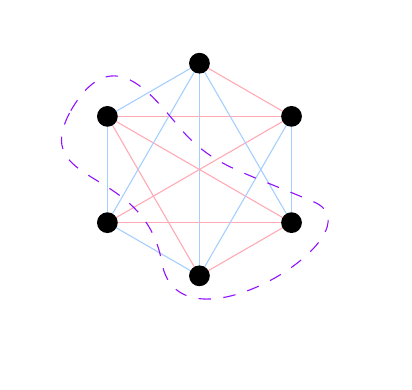
\begin{tikzpicture}[x=0.75pt,y=0.75pt,yscale=-1,xscale=1]
%uncomment if require: \path (0,175); %set diagram left start at 0, and has height of 175

%Straight Lines [id:da17206349312644065] 
\draw [color={rgb, 255:red, 166; green, 207; blue, 255 }  ,draw opacity=1 ]   (233.42,46.36) -- (233.42,148.8) ;
%Straight Lines [id:da12159366505912672] 
\draw [color={rgb, 255:red, 255; green, 171; blue, 181 }  ,draw opacity=1 ]   (277.78,71.97) -- (189.06,123.19) ;
%Straight Lines [id:da5046272832575744] 
\draw [color={rgb, 255:red, 255; green, 171; blue, 181 }  ,draw opacity=1 ]   (277.78,123.19) -- (189.06,71.97) ;
%Straight Lines [id:da5327206246571794] 
\draw [color={rgb, 255:red, 255; green, 171; blue, 181 }  ,draw opacity=1 ]   (277.78,71.97) -- (189.06,71.97) ;
%Straight Lines [id:da5222409079010673] 
\draw [color={rgb, 255:red, 255; green, 171; blue, 181 }  ,draw opacity=1 ]   (277.78,123.19) -- (189.06,123.19) ;
%Straight Lines [id:da5942861899876362] 
\draw [color={rgb, 255:red, 255; green, 171; blue, 181 }  ,draw opacity=1 ]   (189.06,71.97) -- (233.42,148.8) ;
%Straight Lines [id:da5759491047562539] 
\draw [color={rgb, 255:red, 166; green, 207; blue, 255 }  ,draw opacity=1 ]   (277.78,71.97) -- (233.42,148.8) ;
%Straight Lines [id:da8190065405876321] 
\draw [color={rgb, 255:red, 166; green, 207; blue, 255 }  ,draw opacity=1 ]   (233.42,46.36) -- (189.06,123.19) ;
%Straight Lines [id:da6899258654394083] 
\draw [color={rgb, 255:red, 166; green, 207; blue, 255 }  ,draw opacity=1 ]   (233.42,46.36) -- (277.78,123.19) ;
%Straight Lines [id:da6986666640569799] 
\draw [color={rgb, 255:red, 166; green, 207; blue, 255 }  ,draw opacity=1 ]   (189.06,71.97) -- (233.42,46.36) ;
%Straight Lines [id:da8100556514464108] 
\draw [color={rgb, 255:red, 255; green, 171; blue, 181 }  ,draw opacity=1 ]   (233.42,148.8) -- (277.78,123.19) ;
%Straight Lines [id:da7542026700767708] 
\draw [color={rgb, 255:red, 166; green, 207; blue, 255 }  ,draw opacity=1 ]   (277.78,123.19) -- (277.78,71.97) ;
%Straight Lines [id:da04987127034512118] 
\draw [color={rgb, 255:red, 166; green, 207; blue, 255 }  ,draw opacity=1 ]   (189.06,123.19) -- (189.06,71.97) ;
%Straight Lines [id:da32216475387025123] 
\draw [color={rgb, 255:red, 166; green, 207; blue, 255 }  ,draw opacity=1 ]   (233.42,148.8) -- (189.06,123.19) ;
%Straight Lines [id:da26256035573092595] 
\draw [color={rgb, 255:red, 255; green, 171; blue, 181 }  ,draw opacity=1 ]   (277.78,71.97) -- (233.42,46.36) ;
%Shape: Ellipse [id:dp320894690719949] 
\draw  [draw opacity=0][fill={rgb, 255:red, 0; green, 0; blue, 0 }  ,fill opacity=1 ] (272.78,71.97) .. controls (272.78,69.21) and (275.01,66.97) .. (277.78,66.97) .. controls (280.54,66.97) and (282.78,69.21) .. (282.78,71.97) .. controls (282.78,74.73) and (280.54,76.97) .. (277.78,76.97) .. controls (275.01,76.97) and (272.78,74.73) .. (272.78,71.97) -- cycle ;
%Curve Lines [id:da6192278365954909] 
\draw [color={rgb, 255:red, 144; green, 19; blue, 254 }  ,draw opacity=1 ] [dash pattern={on 4.5pt off 4.5pt}]  (171.42,69.27) .. controls (194.34,29.51) and (216.05,71.1) .. (229.95,83.9) .. controls (243.86,96.71) and (254.83,98.9) .. (288.49,113.17) .. controls (322.15,127.44) and (223.61,190) .. (215.32,142.44) .. controls (207.03,94.88) and (150.93,106.59) .. (171.42,69.27) -- cycle ;
%Shape: Ellipse [id:dp15308415995990665] 
\draw  [draw opacity=0][fill={rgb, 255:red, 0; green, 0; blue, 0 }  ,fill opacity=1 ] (272.78,123.19) .. controls (272.78,120.43) and (275.01,118.19) .. (277.78,118.19) .. controls (280.54,118.19) and (282.78,120.43) .. (282.78,123.19) .. controls (282.78,125.95) and (280.54,128.19) .. (277.78,128.19) .. controls (275.01,128.19) and (272.78,125.95) .. (272.78,123.19) -- cycle ;
%Shape: Ellipse [id:dp45955663511934897] 
\draw  [draw opacity=0][fill={rgb, 255:red, 0; green, 0; blue, 0 }  ,fill opacity=1 ] (228.42,148.8) .. controls (228.42,146.04) and (230.66,143.8) .. (233.42,143.8) .. controls (236.18,143.8) and (238.42,146.04) .. (238.42,148.8) .. controls (238.42,151.56) and (236.18,153.8) .. (233.42,153.8) .. controls (230.66,153.8) and (228.42,151.56) .. (228.42,148.8) -- cycle ;
%Shape: Ellipse [id:dp3021339011365316] 
\draw  [draw opacity=0][fill={rgb, 255:red, 0; green, 0; blue, 0 }  ,fill opacity=1 ] (184.06,123.19) .. controls (184.06,120.43) and (186.3,118.19) .. (189.06,118.19) .. controls (191.82,118.19) and (194.06,120.43) .. (194.06,123.19) .. controls (194.06,125.95) and (191.82,128.19) .. (189.06,128.19) .. controls (186.3,128.19) and (184.06,125.95) .. (184.06,123.19) -- cycle ;
%Shape: Ellipse [id:dp43746067344209183] 
\draw  [draw opacity=0][fill={rgb, 255:red, 0; green, 0; blue, 0 }  ,fill opacity=1 ] (184.06,71.97) .. controls (184.06,69.21) and (186.3,66.97) .. (189.06,66.97) .. controls (191.82,66.97) and (194.06,69.21) .. (194.06,71.97) .. controls (194.06,74.73) and (191.82,76.97) .. (189.06,76.97) .. controls (186.3,76.97) and (184.06,74.73) .. (184.06,71.97) -- cycle ;
%Shape: Ellipse [id:dp9805869312234305] 
\draw  [draw opacity=0][fill={rgb, 255:red, 0; green, 0; blue, 0 }  ,fill opacity=1 ] (228.42,46.36) .. controls (228.42,43.6) and (230.66,41.36) .. (233.42,41.36) .. controls (236.18,41.36) and (238.42,43.6) .. (238.42,46.36) .. controls (238.42,49.12) and (236.18,51.36) .. (233.42,51.36) .. controls (230.66,51.36) and (228.42,49.12) .. (228.42,46.36) -- cycle ;




\end{tikzpicture}

	\end{center}
\end{proposition}
\begin{proof}
	Consider some vertex $v$ in the graph. We know that at least three incident edges must be the same colour, so suppose (without loss of generality) that they are red, with endpoints $v_1, v_2, v_3$. Then either $v_1 v_2 v_3$ is a monochromatic blue triangle, or some $v_i v_j$ is red, in which case $v v_i v_j$ is a monochromatic red triangle.
\end{proof}

Straight away we might wonder about $K_4$. Does there exist some large enough $n$ such that every $2-$colouring of $K_n$ contains a monochromatic $K_4$? This is the type of problem we will consider in Ramsey theory.


\subsection{Ramsey Numbers}\label{sec:ramseynums}

We will begin our discussion of Ramsey theory by introducing the \emph{Ramsey numbers}.

\begin{definition}[Ramsey Numbers]
	For $t \in \N$, we define $R(t)$ the \vocab{$t$th Ramsey number} to be the smallest $n$ for which every $2$-colouring of $K_n$ contains a monochromatic $K_t$.
\end{definition}

We already know that $R(3) = 6$ (since we showed there's always a monochromatic triangle in $K_6$, and it's not hard to find a colouring of $K_5$ that doesn't have one). We haven't yet proved though that such an $R(t)$ exists though, so we will clear this up first.

\begin{theorem}[Ramsey's Theorem]
	For all $t \in \N$, $R(t)$ is finite and $R(t) \leq 4^t$.
\end{theorem}
\begin{proof}
	We will begin by proving a small lemma. For $s, t \geq 2$, we define the Ramsey number $R(s, t)$ to be the smallest $n$ such that every red/blue colouring of $K_n$ either contains a red $K_s$ or a blue $K_t$.

	We will prove that for all $s, t \geq 2$,
	\begin{equation}\label{eq:ramsey}
		R(s, t) \leq \binom{s + t - 2}{s - 1}.\tag{$\dagger$}
	\end{equation}

	\emph{Claim}. Assume that $R(s - 1, t)$ and $R(s, t - 1)$ exist. Then $R(s, t)$ exists and $R(s, t) \leq R(s-1, t) + R(s, t - 1)$.

	Let $a = R(s - 1, t)$ and $b = R(s, t - 1)$ and let $c$ be a red/blue colouring of $K_{a + b}$. Let $x$ be a vertex in this graph, and we note $d(x) = a + b - 1$. Then $x$ has either
	\begin{enumerate}[label=(\roman*)]
		\item $a$ red neighbors
		\item $b$ blue neighbors.
	\end{enumerate}
	In case (i), let $N_r$ be the red neighbors of $x$, and note $|N_r| \geq a$. Then the colouring induced on $N_r$ contains either a $K_{s - 1}$ in red or a $K_{t}$ in blue. In the latter case we are done, and in the former case we can add $x$ to $K_{s - 1}$ to finish. Case (ii) is symmetric, and thus our claim is true.

	Now we can return to showing $\eqref{eq:ramsey}$. We are going to induct on $s + t$. Note that $R(s, 2) = s$ and $R(2, t) = t$. Inductively assume that $R(s - 1, t), R(s, t - 1)$ exist and satisfy this relation, then
	$$
	R(s, t) \leq R(s - 1, t) + R(t, s - 1) \leq \binom{s + t - 2}{s - 2} + \binom{s + t - 3}{s - 1} \leq \binom{s + t - 2}{s - 1},
	$$
	as desired. Taking $R(t) = R(t, t)$ gives $R(t) \leq \binom{2t - 2}{t - 1} \leq 4^t$.
\end{proof}

Ramsey numbers are generally quite mysterious.
We know for example that
$R(3,3) = 6$, $R(4,4) = 18$, and $R(3,7) = 23$, 
but even something like $R(5, 5)$ is unknown, and our best bounds are $43 \leq R(5, 5) \leq 48$. The numbers $R(3, t)$ are quite well understood, and for $\epsilon > 0$ we have (for sufficiently large $t$)
$$
\left(\frac{1}{4}+\varepsilon\right) \frac{t^{2}}{\log t} \leqslant R(3, t) \leqslant(1+\varepsilon) \frac{t^{2}}{\log t}.
$$

A big question though is getting a lower bound on $R(t)$, which is currently nowhere as close as our upper bound.


\subsection{Infinite Ramsey}

Now instead of finite complete graphs, we are going to consider an infinite graph.

\begin{definition}[Complete Countable Graph]
	We define the \vocab{complete countable graph} $G = (\N, \N^{(2)})$.
\end{definition}

\begin{notation}
	For a set $X$, we let $X^{(r)} = \{A \subseteq X \mid |A| = r\}$, the set of $r$ element subsets of $X$.
\end{notation}

Our motivating question will be the following: given a 2-colouring of the complete countable graph, what can we say about the monochromatic structures that appear in the colouring? Obviously by Ramsey's theorem we can find arbitrarily large monochromatic complete graphs, but is it possible to find a monochromatic complete countable subgraph?

\begin{example}[Complete Countable Graph with Complete Countable Subgraph]
	Consider the colouring of a complete countable graph where $xy$ is red if $x + y$ is even, and blue if $x + y$ is odd.
	Then the subgraph induced on the vertices $\{2, 4, 8, \dots\}$ is a monochromatic complete countable subgraph.

	Now consider instead the colouring where $x + y$ is red if it has an even number of prime factors, and $x + y$ is blue if it has an odd number of prime factors. Can you find a monochromatic complete countable subgraph?
\end{example}

It turns out that by another theorem of Ramsey, it is always possible to find such a subgraph.

\begin{theorem}[Infinite Ramsey's Theorem]
	Let $G= (\N, \N^{(2)})$, the complete countable graph. Then for every 2-colouring of $G$ there exists an infinite set $X \subseteq \N$ so that $X^{(2)}$ is monochromatic.
\end{theorem}
\begin{proof}
	We begin by inductively defining vertices $x_1, x_2, \dots, x_t$ and colours $c_1, c_2, \dots, c_t$ such that 
	$N_{c_i}(x_i) \supset \{x_{i + 1}, \dots, x_{t}\},$
	and
	$
	\bigcap_{i = 1}^t N_{c_i}(x_i)
	$ is infinite, where $N_{c_i}(x_i)$ is the neighborhood of $x_i$ in the colour $c_i$.

	We can do this by taking $x_1, \dots, x_t$ and then choosing any $x_{t + 1} \in \bigcap_{i = 1}^t N_{c_i}(x_i)$. Then we can define $c_i$ accordingly, since at least one of $N_{red}(x_{t + 1}) \cap \left(\bigcap_{i = 1}^t N_{c_i}(x_i)\right)$ is infinite, or $N_{blue}(x_{t + 1}) \cap \left(\bigcap_{i = 1}^t N_{c_i}(x_i)\right)$ is infinite.

	This then gives us an infinite collection $x_1, x_2, \dots$ so that $x_i x_j$ with $i < j$ are given colour $c_i$. Then since both
	$$
	\{x_i \mid c_i = \text{red}\} \quad \text{and} \quad \{x_i \mid c_i = \text{blue}\}
	$$
	are monochromatic cliques, at least one of them is infinite, giving a monochromatic complete countable subgraph.
\end{proof}

\begin{remark}
	By keeping track of the sizes of sets at each step, we can adapt this proof to give us a different proof of the finite case.
\end{remark}

\subsection{Ramsey Numbers for Hypergraphs}

Before, we were colouring $X^{(2)}$, the pairs of a set $X$ (the vertices of a graph). Of course, we might wonder what happens when we colour $r$-sets?

\begin{definition}[Hypergraph Ramsey Numbers]
	We define $R^{(r)}(s, t)$ to be the smallest $n$ such that every red/blue colouring of $[n]^{(r)}$ either contains a set $X \subseteq [n]$ with $|X| = s$ and $X^{(r)}$ red, or there exists $Y \subseteq[n]$ with $|Y| = t$ and $Y^{(r)}$ blue.
\end{definition}

And of course, it's not guaranteed that these exist, but it is possible to show that they do.

\begin{theorem}[Hypergraph Ramsey Theorem]
	For all $r, s, t \geq 2$, $R^{(r)}(s, t)$ exists.
\end{theorem}
\begin{proof}
	Omitted.\let\qed\relax
\end{proof}

\subsection{Lower Bounds for Ramsey Numbers}

We said and the end of \autoref{sec:ramseynums} that we were left to get a good lower bound on the Ramsey numbers $R(t)$. One way to do that might be by considering the following extremal-seeming construction:

\begin{center}
	

\tikzset{every picture/.style={line width=0.75pt}} %set default line width to 0.75pt        

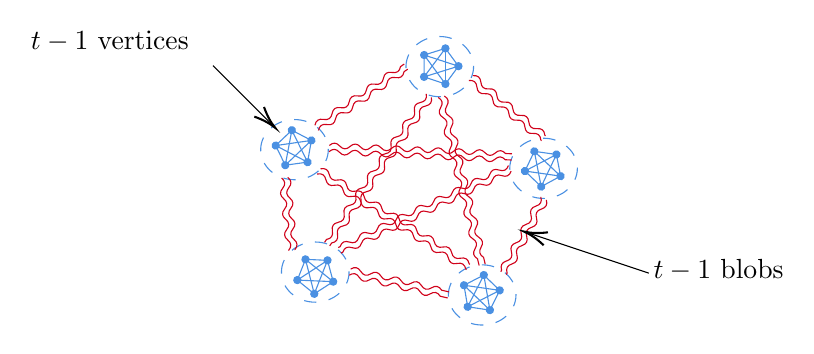
\begin{tikzpicture}[x=0.75pt,y=0.75pt,yscale=-1,xscale=1]
%uncomment if require: \path (0,237); %set diagram left start at 0, and has height of 237

%Shape: Ellipse [id:dp260229253449785] 
\draw  [color={rgb, 255:red, 74; green, 144; blue, 226 }  ,draw opacity=1 ][fill={rgb, 255:red, 74; green, 144; blue, 226 }  ,fill opacity=1 ] (158.68,79.29) .. controls (158.27,78.44) and (158.62,77.42) .. (159.46,77) .. controls (160.31,76.58) and (161.34,76.93) .. (161.76,77.78) .. controls (162.18,78.63) and (161.83,79.66) .. (160.98,80.07) .. controls (160.13,80.49) and (159.1,80.14) .. (158.68,79.29) -- cycle ;
%Shape: Ellipse [id:dp8425132311806203] 
\draw  [color={rgb, 255:red, 74; green, 144; blue, 226 }  ,draw opacity=1 ][fill={rgb, 255:red, 74; green, 144; blue, 226 }  ,fill opacity=1 ] (166.47,71.9) .. controls (166.05,71.05) and (166.4,70.02) .. (167.25,69.6) .. controls (168.1,69.18) and (169.13,69.53) .. (169.55,70.38) .. controls (169.97,71.23) and (169.62,72.26) .. (168.77,72.68) .. controls (167.92,73.1) and (166.89,72.75) .. (166.47,71.9) -- cycle ;
%Shape: Ellipse [id:dp45548962134158066] 
\draw  [color={rgb, 255:red, 74; green, 144; blue, 226 }  ,draw opacity=1 ][fill={rgb, 255:red, 74; green, 144; blue, 226 }  ,fill opacity=1 ] (163.3,88.74) .. controls (162.88,87.89) and (163.23,86.87) .. (164.08,86.45) .. controls (164.93,86.03) and (165.96,86.38) .. (166.37,87.23) .. controls (166.79,88.08) and (166.44,89.11) .. (165.59,89.53) .. controls (164.74,89.94) and (163.72,89.59) .. (163.3,88.74) -- cycle ;
%Shape: Ellipse [id:dp07259317563355205] 
\draw  [color={rgb, 255:red, 74; green, 144; blue, 226 }  ,draw opacity=1 ][fill={rgb, 255:red, 74; green, 144; blue, 226 }  ,fill opacity=1 ] (174.04,87.28) .. controls (173.62,86.43) and (173.97,85.4) .. (174.82,84.98) .. controls (175.67,84.57) and (176.7,84.92) .. (177.12,85.77) .. controls (177.54,86.61) and (177.19,87.64) .. (176.34,88.06) .. controls (175.49,88.48) and (174.46,88.13) .. (174.04,87.28) -- cycle ;
%Shape: Ellipse [id:dp7294194533979528] 
\draw  [color={rgb, 255:red, 74; green, 144; blue, 226 }  ,draw opacity=1 ][fill={rgb, 255:red, 74; green, 144; blue, 226 }  ,fill opacity=1 ] (175.9,76.81) .. controls (175.48,75.96) and (175.83,74.94) .. (176.68,74.52) .. controls (177.53,74.1) and (178.55,74.45) .. (178.97,75.3) .. controls (179.39,76.15) and (179.04,77.18) .. (178.19,77.59) .. controls (177.34,78.01) and (176.31,77.66) .. (175.9,76.81) -- cycle ;
%Straight Lines [id:da7144000673669442] 
\draw [color={rgb, 255:red, 74; green, 144; blue, 226 }  ,draw opacity=1 ]   (160.22,78.54) -- (168.01,71.14) ;
%Straight Lines [id:da8565951395139575] 
\draw [color={rgb, 255:red, 74; green, 144; blue, 226 }  ,draw opacity=1 ]   (164.84,87.99) -- (177.43,76.06) ;
%Straight Lines [id:da6570259060714745] 
\draw [color={rgb, 255:red, 74; green, 144; blue, 226 }  ,draw opacity=1 ]   (175.58,86.52) -- (168.01,71.14) ;
%Straight Lines [id:da040467557102866536] 
\draw [color={rgb, 255:red, 74; green, 144; blue, 226 }  ,draw opacity=1 ]   (177.43,76.06) -- (168.01,71.14) ;
%Straight Lines [id:da5079914482287651] 
\draw [color={rgb, 255:red, 74; green, 144; blue, 226 }  ,draw opacity=1 ]   (175.58,86.52) -- (164.84,87.99) ;
%Straight Lines [id:da9083204720233942] 
\draw [color={rgb, 255:red, 74; green, 144; blue, 226 }  ,draw opacity=1 ]   (177.43,76.06) -- (175.58,86.52) ;
%Straight Lines [id:da03417651457849913] 
\draw [color={rgb, 255:red, 74; green, 144; blue, 226 }  ,draw opacity=1 ]   (168.01,71.14) -- (164.84,87.99) ;
%Straight Lines [id:da6115204676544925] 
\draw [color={rgb, 255:red, 74; green, 144; blue, 226 }  ,draw opacity=1 ]   (177.43,76.06) -- (160.22,78.54) ;
%Straight Lines [id:da6394603510865864] 
\draw [color={rgb, 255:red, 74; green, 144; blue, 226 }  ,draw opacity=1 ]   (175.58,86.52) -- (160.22,78.54) ;
%Straight Lines [id:da04814829836751677] 
\draw [color={rgb, 255:red, 74; green, 144; blue, 226 }  ,draw opacity=1 ]   (164.84,87.99) -- (160.22,78.54) ;

%Shape: Ellipse [id:dp9751004381027886] 
\draw  [color={rgb, 255:red, 74; green, 144; blue, 226 }  ,draw opacity=1 ][fill={rgb, 255:red, 74; green, 144; blue, 226 }  ,fill opacity=1 ] (230.03,34.91) .. controls (230.03,33.96) and (230.8,33.2) .. (231.75,33.2) .. controls (232.69,33.2) and (233.46,33.96) .. (233.46,34.91) .. controls (233.46,35.86) and (232.69,36.63) .. (231.75,36.63) .. controls (230.8,36.63) and (230.03,35.86) .. (230.03,34.91) -- cycle ;
%Shape: Ellipse [id:dp08336940380025415] 
\draw  [color={rgb, 255:red, 74; green, 144; blue, 226 }  ,draw opacity=1 ][fill={rgb, 255:red, 74; green, 144; blue, 226 }  ,fill opacity=1 ] (240.29,31.71) .. controls (240.29,30.77) and (241.05,30) .. (242,30) .. controls (242.95,30) and (243.71,30.77) .. (243.71,31.71) .. controls (243.71,32.66) and (242.95,33.43) .. (242,33.43) .. controls (241.05,33.43) and (240.29,32.66) .. (240.29,31.71) -- cycle ;
%Shape: Ellipse [id:dp6358542806423357] 
\draw  [color={rgb, 255:red, 74; green, 144; blue, 226 }  ,draw opacity=1 ][fill={rgb, 255:red, 74; green, 144; blue, 226 }  ,fill opacity=1 ] (230,45.43) .. controls (230,44.48) and (230.77,43.71) .. (231.71,43.71) .. controls (232.66,43.71) and (233.43,44.48) .. (233.43,45.43) .. controls (233.43,46.38) and (232.66,47.14) .. (231.71,47.14) .. controls (230.77,47.14) and (230,46.38) .. (230,45.43) -- cycle ;
%Shape: Ellipse [id:dp6009669519413119] 
\draw  [color={rgb, 255:red, 74; green, 144; blue, 226 }  ,draw opacity=1 ][fill={rgb, 255:red, 74; green, 144; blue, 226 }  ,fill opacity=1 ] (240.29,48.86) .. controls (240.29,47.91) and (241.05,47.14) .. (242,47.14) .. controls (242.95,47.14) and (243.71,47.91) .. (243.71,48.86) .. controls (243.71,49.8) and (242.95,50.57) .. (242,50.57) .. controls (241.05,50.57) and (240.29,49.8) .. (240.29,48.86) -- cycle ;
%Shape: Ellipse [id:dp5849992851094483] 
\draw  [color={rgb, 255:red, 74; green, 144; blue, 226 }  ,draw opacity=1 ][fill={rgb, 255:red, 74; green, 144; blue, 226 }  ,fill opacity=1 ] (246.57,40.29) .. controls (246.57,39.34) and (247.34,38.57) .. (248.29,38.57) .. controls (249.23,38.57) and (250,39.34) .. (250,40.29) .. controls (250,41.23) and (249.23,42) .. (248.29,42) .. controls (247.34,42) and (246.57,41.23) .. (246.57,40.29) -- cycle ;
%Straight Lines [id:da20682623652269672] 
\draw [color={rgb, 255:red, 74; green, 144; blue, 226 }  ,draw opacity=1 ]   (231.75,34.91) -- (242,31.71) ;
%Straight Lines [id:da4531828113723517] 
\draw [color={rgb, 255:red, 74; green, 144; blue, 226 }  ,draw opacity=1 ]   (231.71,45.43) -- (248.29,40.29) ;
%Straight Lines [id:da7934487600375209] 
\draw [color={rgb, 255:red, 74; green, 144; blue, 226 }  ,draw opacity=1 ]   (242,48.86) -- (242,31.71) ;
%Straight Lines [id:da04911061541929507] 
\draw [color={rgb, 255:red, 74; green, 144; blue, 226 }  ,draw opacity=1 ]   (248.29,40.29) -- (242,31.71) ;
%Straight Lines [id:da055562590112089305] 
\draw [color={rgb, 255:red, 74; green, 144; blue, 226 }  ,draw opacity=1 ]   (242,48.86) -- (231.71,45.43) ;
%Straight Lines [id:da03782964265871902] 
\draw [color={rgb, 255:red, 74; green, 144; blue, 226 }  ,draw opacity=1 ]   (248.29,40.29) -- (242,48.86) ;
%Straight Lines [id:da21893265825490138] 
\draw [color={rgb, 255:red, 74; green, 144; blue, 226 }  ,draw opacity=1 ]   (242,31.71) -- (231.71,45.43) ;
%Straight Lines [id:da5165557514850139] 
\draw [color={rgb, 255:red, 74; green, 144; blue, 226 }  ,draw opacity=1 ]   (248.29,40.29) -- (231.75,34.91) ;
%Straight Lines [id:da9940901111329599] 
\draw [color={rgb, 255:red, 74; green, 144; blue, 226 }  ,draw opacity=1 ]   (242,48.86) -- (231.75,34.91) ;
%Straight Lines [id:da18788686876570448] 
\draw [color={rgb, 255:red, 74; green, 144; blue, 226 }  ,draw opacity=1 ]   (231.71,45.43) -- (231.75,34.91) ;

%Shape: Ellipse [id:dp7459314683532199] 
\draw  [color={rgb, 255:red, 74; green, 144; blue, 226 }  ,draw opacity=1 ][fill={rgb, 255:red, 74; green, 144; blue, 226 }  ,fill opacity=1 ] (283.29,80.59) .. controls (283.7,79.73) and (284.72,79.37) .. (285.58,79.77) .. controls (286.43,80.18) and (286.8,81.2) .. (286.39,82.06) .. controls (285.99,82.91) and (284.96,83.28) .. (284.11,82.87) .. controls (283.25,82.47) and (282.89,81.45) .. (283.29,80.59) -- cycle ;
%Shape: Ellipse [id:dp07428000047575378] 
\draw  [color={rgb, 255:red, 74; green, 144; blue, 226 }  ,draw opacity=1 ][fill={rgb, 255:red, 74; green, 144; blue, 226 }  ,fill opacity=1 ] (293.93,82.09) .. controls (294.33,81.23) and (295.36,80.87) .. (296.21,81.28) .. controls (297.07,81.68) and (297.43,82.7) .. (297.03,83.56) .. controls (296.62,84.41) and (295.6,84.78) .. (294.74,84.37) .. controls (293.89,83.97) and (293.52,82.95) .. (293.93,82.09) -- cycle ;
%Shape: Ellipse [id:dp22961158641347668] 
\draw  [color={rgb, 255:red, 74; green, 144; blue, 226 }  ,draw opacity=1 ][fill={rgb, 255:red, 74; green, 144; blue, 226 }  ,fill opacity=1 ] (278.76,90.08) .. controls (279.17,89.22) and (280.19,88.86) .. (281.04,89.27) .. controls (281.9,89.67) and (282.26,90.69) .. (281.86,91.55) .. controls (281.45,92.4) and (280.43,92.77) .. (279.58,92.36) .. controls (278.72,91.96) and (278.36,90.94) .. (278.76,90.08) -- cycle ;
%Shape: Ellipse [id:dp08080032347891208] 
\draw  [color={rgb, 255:red, 74; green, 144; blue, 226 }  ,draw opacity=1 ][fill={rgb, 255:red, 74; green, 144; blue, 226 }  ,fill opacity=1 ] (286.59,97.58) .. controls (286.99,96.73) and (288.02,96.36) .. (288.87,96.77) .. controls (289.73,97.17) and (290.09,98.2) .. (289.69,99.05) .. controls (289.28,99.91) and (288.26,100.27) .. (287.4,99.87) .. controls (286.55,99.46) and (286.18,98.44) .. (286.59,97.58) -- cycle ;
%Shape: Ellipse [id:dp4842286508628091] 
\draw  [color={rgb, 255:red, 74; green, 144; blue, 226 }  ,draw opacity=1 ][fill={rgb, 255:red, 74; green, 144; blue, 226 }  ,fill opacity=1 ] (295.94,92.53) .. controls (296.34,91.67) and (297.37,91.31) .. (298.22,91.71) .. controls (299.08,92.12) and (299.44,93.14) .. (299.04,94) .. controls (298.63,94.85) and (297.61,95.22) .. (296.75,94.81) .. controls (295.9,94.41) and (295.53,93.38) .. (295.94,92.53) -- cycle ;
%Straight Lines [id:da3255647700302482] 
\draw [color={rgb, 255:red, 74; green, 144; blue, 226 }  ,draw opacity=1 ]   (284.84,81.32) -- (295.48,82.82) ;
%Straight Lines [id:da9547718599308663] 
\draw [color={rgb, 255:red, 74; green, 144; blue, 226 }  ,draw opacity=1 ]   (280.31,90.81) -- (297.49,93.26) ;
%Straight Lines [id:da9905389969362575] 
\draw [color={rgb, 255:red, 74; green, 144; blue, 226 }  ,draw opacity=1 ]   (288.14,98.32) -- (295.48,82.82) ;
%Straight Lines [id:da55372685390663] 
\draw [color={rgb, 255:red, 74; green, 144; blue, 226 }  ,draw opacity=1 ]   (297.49,93.26) -- (295.48,82.82) ;
%Straight Lines [id:da9557897471757337] 
\draw [color={rgb, 255:red, 74; green, 144; blue, 226 }  ,draw opacity=1 ]   (288.14,98.32) -- (280.31,90.81) ;
%Straight Lines [id:da36574651524646207] 
\draw [color={rgb, 255:red, 74; green, 144; blue, 226 }  ,draw opacity=1 ]   (297.49,93.26) -- (288.14,98.32) ;
%Straight Lines [id:da42272588853782866] 
\draw [color={rgb, 255:red, 74; green, 144; blue, 226 }  ,draw opacity=1 ]   (295.48,82.82) -- (280.31,90.81) ;
%Straight Lines [id:da7047171024571248] 
\draw [color={rgb, 255:red, 74; green, 144; blue, 226 }  ,draw opacity=1 ]   (297.49,93.26) -- (284.84,81.32) ;
%Straight Lines [id:da6456705914266825] 
\draw [color={rgb, 255:red, 74; green, 144; blue, 226 }  ,draw opacity=1 ]   (288.14,98.32) -- (284.84,81.32) ;
%Straight Lines [id:da0822942276495926] 
\draw [color={rgb, 255:red, 74; green, 144; blue, 226 }  ,draw opacity=1 ]   (280.31,90.81) -- (284.84,81.32) ;

%Shape: Ellipse [id:dp5199960746315602] 
\draw  [color={rgb, 255:red, 74; green, 144; blue, 226 }  ,draw opacity=1 ][fill={rgb, 255:red, 74; green, 144; blue, 226 }  ,fill opacity=1 ] (249.26,146.13) .. controls (249.1,145.2) and (249.72,144.31) .. (250.65,144.15) .. controls (251.59,143.98) and (252.47,144.61) .. (252.64,145.54) .. controls (252.8,146.47) and (252.17,147.36) .. (251.24,147.52) .. controls (250.31,147.69) and (249.42,147.06) .. (249.26,146.13) -- cycle ;
%Shape: Ellipse [id:dp6303304363712059] 
\draw  [color={rgb, 255:red, 74; green, 144; blue, 226 }  ,draw opacity=1 ][fill={rgb, 255:red, 74; green, 144; blue, 226 }  ,fill opacity=1 ] (258.81,141.22) .. controls (258.65,140.29) and (259.27,139.4) .. (260.21,139.24) .. controls (261.14,139.08) and (262.03,139.7) .. (262.19,140.63) .. controls (262.35,141.57) and (261.73,142.45) .. (260.79,142.62) .. controls (259.86,142.78) and (258.97,142.15) .. (258.81,141.22) -- cycle ;
%Shape: Ellipse [id:dp411029732542481] 
\draw  [color={rgb, 255:red, 74; green, 144; blue, 226 }  ,draw opacity=1 ][fill={rgb, 255:red, 74; green, 144; blue, 226 }  ,fill opacity=1 ] (251.03,156.5) .. controls (250.87,155.56) and (251.49,154.67) .. (252.42,154.51) .. controls (253.36,154.35) and (254.25,154.97) .. (254.41,155.91) .. controls (254.57,156.84) and (253.95,157.73) .. (253.01,157.89) .. controls (252.08,158.05) and (251.19,157.43) .. (251.03,156.5) -- cycle ;
%Shape: Ellipse [id:dp8388759040474085] 
\draw  [color={rgb, 255:red, 74; green, 144; blue, 226 }  ,draw opacity=1 ][fill={rgb, 255:red, 74; green, 144; blue, 226 }  ,fill opacity=1 ] (261.75,158.11) .. controls (261.59,157.18) and (262.21,156.29) .. (263.15,156.13) .. controls (264.08,155.96) and (264.97,156.59) .. (265.13,157.52) .. controls (265.29,158.45) and (264.67,159.34) .. (263.73,159.5) .. controls (262.8,159.67) and (261.91,159.04) .. (261.75,158.11) -- cycle ;
%Shape: Ellipse [id:dp7536302204609595] 
\draw  [color={rgb, 255:red, 74; green, 144; blue, 226 }  ,draw opacity=1 ][fill={rgb, 255:red, 74; green, 144; blue, 226 }  ,fill opacity=1 ] (266.47,148.59) .. controls (266.31,147.66) and (266.94,146.77) .. (267.87,146.61) .. controls (268.8,146.44) and (269.69,147.07) .. (269.85,148) .. controls (270.01,148.93) and (269.39,149.82) .. (268.46,149.98) .. controls (267.52,150.15) and (266.64,149.52) .. (266.47,148.59) -- cycle ;
%Straight Lines [id:da6564285448526064] 
\draw [color={rgb, 255:red, 74; green, 144; blue, 226 }  ,draw opacity=1 ]   (250.95,145.83) -- (260.5,140.93) ;
%Straight Lines [id:da3599466331126684] 
\draw [color={rgb, 255:red, 74; green, 144; blue, 226 }  ,draw opacity=1 ]   (252.72,156.2) -- (268.16,148.29) ;
%Straight Lines [id:da243782972113312] 
\draw [color={rgb, 255:red, 74; green, 144; blue, 226 }  ,draw opacity=1 ]   (263.44,157.82) -- (260.5,140.93) ;
%Straight Lines [id:da8998950142746327] 
\draw [color={rgb, 255:red, 74; green, 144; blue, 226 }  ,draw opacity=1 ]   (268.16,148.29) -- (260.5,140.93) ;
%Straight Lines [id:da6595957805041219] 
\draw [color={rgb, 255:red, 74; green, 144; blue, 226 }  ,draw opacity=1 ]   (263.44,157.82) -- (252.72,156.2) ;
%Straight Lines [id:da7145730221721425] 
\draw [color={rgb, 255:red, 74; green, 144; blue, 226 }  ,draw opacity=1 ]   (268.16,148.29) -- (263.44,157.82) ;
%Straight Lines [id:da2628869253558477] 
\draw [color={rgb, 255:red, 74; green, 144; blue, 226 }  ,draw opacity=1 ]   (260.5,140.93) -- (252.72,156.2) ;
%Straight Lines [id:da3475364061788526] 
\draw [color={rgb, 255:red, 74; green, 144; blue, 226 }  ,draw opacity=1 ]   (268.16,148.29) -- (250.95,145.83) ;
%Straight Lines [id:da9824484438670134] 
\draw [color={rgb, 255:red, 74; green, 144; blue, 226 }  ,draw opacity=1 ]   (263.44,157.82) -- (250.95,145.83) ;
%Straight Lines [id:da4638969701340634] 
\draw [color={rgb, 255:red, 74; green, 144; blue, 226 }  ,draw opacity=1 ]   (252.72,156.2) -- (250.95,145.83) ;

%Shape: Ellipse [id:dp4566740728411707] 
\draw  [color={rgb, 255:red, 74; green, 144; blue, 226 }  ,draw opacity=1 ][fill={rgb, 255:red, 74; green, 144; blue, 226 }  ,fill opacity=1 ] (169.56,144.68) .. controls (168.83,144.09) and (168.71,143.01) .. (169.3,142.27) .. controls (169.9,141.54) and (170.98,141.42) .. (171.71,142.01) .. controls (172.45,142.61) and (172.57,143.68) .. (171.97,144.42) .. controls (171.38,145.16) and (170.3,145.28) .. (169.56,144.68) -- cycle ;
%Shape: Ellipse [id:dp6638878936105996] 
\draw  [color={rgb, 255:red, 74; green, 144; blue, 226 }  ,draw opacity=1 ][fill={rgb, 255:red, 74; green, 144; blue, 226 }  ,fill opacity=1 ] (173.5,134.69) .. controls (172.76,134.1) and (172.65,133.02) .. (173.24,132.28) .. controls (173.83,131.54) and (174.91,131.43) .. (175.65,132.02) .. controls (176.39,132.61) and (176.5,133.69) .. (175.91,134.43) .. controls (175.32,135.17) and (174.24,135.28) .. (173.5,134.69) -- cycle ;
%Shape: Ellipse [id:dp8066878410162388] 
\draw  [color={rgb, 255:red, 74; green, 144; blue, 226 }  ,draw opacity=1 ][fill={rgb, 255:red, 74; green, 144; blue, 226 }  ,fill opacity=1 ] (177.74,151.3) .. controls (177,150.71) and (176.88,149.63) .. (177.48,148.89) .. controls (178.07,148.15) and (179.15,148.04) .. (179.89,148.63) .. controls (180.63,149.22) and (180.74,150.3) .. (180.15,151.04) .. controls (179.55,151.78) and (178.48,151.89) .. (177.74,151.3) -- cycle ;
%Shape: Ellipse [id:dp2096738009032293] 
\draw  [color={rgb, 255:red, 74; green, 144; blue, 226 }  ,draw opacity=1 ][fill={rgb, 255:red, 74; green, 144; blue, 226 }  ,fill opacity=1 ] (186.86,145.44) .. controls (186.12,144.84) and (186,143.76) .. (186.6,143.03) .. controls (187.19,142.29) and (188.27,142.17) .. (189.01,142.77) .. controls (189.74,143.36) and (189.86,144.44) .. (189.27,145.18) .. controls (188.67,145.91) and (187.59,146.03) .. (186.86,145.44) -- cycle ;
%Shape: Ellipse [id:dp5256775011012556] 
\draw  [color={rgb, 255:red, 74; green, 144; blue, 226 }  ,draw opacity=1 ][fill={rgb, 255:red, 74; green, 144; blue, 226 }  ,fill opacity=1 ] (184.12,135.17) .. controls (183.38,134.57) and (183.26,133.49) .. (183.86,132.76) .. controls (184.45,132.02) and (185.53,131.9) .. (186.27,132.49) .. controls (187.01,133.09) and (187.12,134.17) .. (186.53,134.9) .. controls (185.94,135.64) and (184.86,135.76) .. (184.12,135.17) -- cycle ;
%Straight Lines [id:da6463826998495803] 
\draw [color={rgb, 255:red, 74; green, 144; blue, 226 }  ,draw opacity=1 ]   (170.64,143.35) -- (174.58,133.35) ;
%Straight Lines [id:da7449651497254464] 
\draw [color={rgb, 255:red, 74; green, 144; blue, 226 }  ,draw opacity=1 ]   (178.81,149.97) -- (185.19,133.83) ;
%Straight Lines [id:da8742339331703968] 
\draw [color={rgb, 255:red, 74; green, 144; blue, 226 }  ,draw opacity=1 ]   (187.93,144.1) -- (174.58,133.35) ;
%Straight Lines [id:da3783434637024088] 
\draw [color={rgb, 255:red, 74; green, 144; blue, 226 }  ,draw opacity=1 ]   (185.19,133.83) -- (174.58,133.35) ;
%Straight Lines [id:da8876396846804981] 
\draw [color={rgb, 255:red, 74; green, 144; blue, 226 }  ,draw opacity=1 ]   (187.93,144.1) -- (178.81,149.97) ;
%Straight Lines [id:da8388661543593503] 
\draw [color={rgb, 255:red, 74; green, 144; blue, 226 }  ,draw opacity=1 ]   (185.19,133.83) -- (187.93,144.1) ;
%Straight Lines [id:da7606860358500784] 
\draw [color={rgb, 255:red, 74; green, 144; blue, 226 }  ,draw opacity=1 ]   (174.58,133.35) -- (178.81,149.97) ;
%Straight Lines [id:da4308618876662216] 
\draw [color={rgb, 255:red, 74; green, 144; blue, 226 }  ,draw opacity=1 ]   (185.19,133.83) -- (170.64,143.35) ;
%Straight Lines [id:da1035202399084203] 
\draw [color={rgb, 255:red, 74; green, 144; blue, 226 }  ,draw opacity=1 ]   (187.93,144.1) -- (170.64,143.35) ;
%Straight Lines [id:da5303999125113144] 
\draw [color={rgb, 255:red, 74; green, 144; blue, 226 }  ,draw opacity=1 ]   (178.81,149.97) -- (170.64,143.35) ;

%Shape: Ellipse [id:dp6329445093609554] 
\draw  [color={rgb, 255:red, 74; green, 144; blue, 226 }  ,draw opacity=1 ][dash pattern={on 4.5pt off 4.5pt}] (153,80.5) .. controls (153,72.49) and (160.29,66) .. (169.29,66) .. controls (178.28,66) and (185.57,72.49) .. (185.57,80.5) .. controls (185.57,88.51) and (178.28,95) .. (169.29,95) .. controls (160.29,95) and (153,88.51) .. (153,80.5) -- cycle ;
%Shape: Ellipse [id:dp7946258711333409] 
\draw  [color={rgb, 255:red, 74; green, 144; blue, 226 }  ,draw opacity=1 ][dash pattern={on 4.5pt off 4.5pt}] (163,139.5) .. controls (163,131.49) and (170.29,125) .. (179.29,125) .. controls (188.28,125) and (195.57,131.49) .. (195.57,139.5) .. controls (195.57,147.51) and (188.28,154) .. (179.29,154) .. controls (170.29,154) and (163,147.51) .. (163,139.5) -- cycle ;
%Shape: Ellipse [id:dp35919509302445873] 
\draw  [color={rgb, 255:red, 74; green, 144; blue, 226 }  ,draw opacity=1 ][dash pattern={on 4.5pt off 4.5pt}] (243.43,150.5) .. controls (243.43,142.49) and (250.72,136) .. (259.71,136) .. controls (268.71,136) and (276,142.49) .. (276,150.5) .. controls (276,158.51) and (268.71,165) .. (259.71,165) .. controls (250.72,165) and (243.43,158.51) .. (243.43,150.5) -- cycle ;
%Shape: Ellipse [id:dp5037517138484366] 
\draw  [color={rgb, 255:red, 74; green, 144; blue, 226 }  ,draw opacity=1 ][dash pattern={on 4.5pt off 4.5pt}] (273,89.5) .. controls (273,81.49) and (280.29,75) .. (289.29,75) .. controls (298.28,75) and (305.57,81.49) .. (305.57,89.5) .. controls (305.57,97.51) and (298.28,104) .. (289.29,104) .. controls (280.29,104) and (273,97.51) .. (273,89.5) -- cycle ;
%Shape: Ellipse [id:dp20984583845028149] 
\draw  [color={rgb, 255:red, 74; green, 144; blue, 226 }  ,draw opacity=1 ][dash pattern={on 4.5pt off 4.5pt}] (223,40.5) .. controls (223,32.49) and (230.29,26) .. (239.29,26) .. controls (248.28,26) and (255.57,32.49) .. (255.57,40.5) .. controls (255.57,48.51) and (248.28,55) .. (239.29,55) .. controls (230.29,55) and (223,48.51) .. (223,40.5) -- cycle ;
%Straight Lines [id:da4619065394796944] 
\draw [color={rgb, 255:red, 208; green, 2; blue, 27 }  ,draw opacity=1 ]   (179.15,68.76) .. controls (179.58,66.45) and (180.95,65.5) .. (183.27,65.93) .. controls (185.58,66.36) and (186.96,65.42) .. (187.4,63.11) .. controls (187.83,60.79) and (189.2,59.85) .. (191.52,60.28) .. controls (193.84,60.71) and (195.21,59.77) .. (195.64,57.45) .. controls (196.07,55.13) and (197.45,54.19) .. (199.77,54.62) .. controls (202.09,55.05) and (203.46,54.11) .. (203.89,51.79) .. controls (204.32,49.47) and (205.69,48.53) .. (208.01,48.96) .. controls (210.33,49.39) and (211.71,48.45) .. (212.14,46.13) .. controls (212.57,43.82) and (213.95,42.88) .. (216.26,43.31) .. controls (218.58,43.74) and (219.95,42.8) .. (220.38,40.48) -- (222.15,39.26) -- (222.15,39.26)(180.85,71.24) .. controls (181.28,68.92) and (182.66,67.98) .. (184.97,68.41) .. controls (187.29,68.84) and (188.66,67.9) .. (189.09,65.58) .. controls (189.52,63.26) and (190.9,62.32) .. (193.22,62.75) .. controls (195.54,63.18) and (196.91,62.24) .. (197.34,59.92) .. controls (197.77,57.6) and (199.14,56.66) .. (201.46,57.09) .. controls (203.77,57.52) and (205.15,56.58) .. (205.59,54.27) .. controls (206.02,51.95) and (207.39,51.01) .. (209.71,51.44) .. controls (212.03,51.87) and (213.4,50.93) .. (213.83,48.61) .. controls (214.26,46.29) and (215.64,45.35) .. (217.96,45.78) .. controls (220.28,46.21) and (221.65,45.27) .. (222.08,42.95) -- (223.85,41.74) -- (223.85,41.74) ;
%Straight Lines [id:da9012241880594938] 
\draw [color={rgb, 255:red, 208; green, 2; blue, 27 }  ,draw opacity=1 ]   (196.34,138.04) .. controls (198.34,136.79) and (199.96,137.17) .. (201.21,139.17) .. controls (202.46,141.17) and (204.08,141.55) .. (206.08,140.3) .. controls (208.08,139.05) and (209.7,139.43) .. (210.95,141.43) .. controls (212.2,143.43) and (213.82,143.81) .. (215.82,142.56) .. controls (217.82,141.31) and (219.44,141.69) .. (220.69,143.69) .. controls (221.94,145.69) and (223.56,146.07) .. (225.56,144.82) .. controls (227.56,143.57) and (229.18,143.95) .. (230.43,145.95) .. controls (231.68,147.95) and (233.3,148.33) .. (235.3,147.08) .. controls (237.3,145.83) and (238.93,146.21) .. (240.18,148.21) -- (243.77,149.04) -- (243.77,149.04)(195.66,140.96) .. controls (197.66,139.71) and (199.28,140.09) .. (200.53,142.09) .. controls (201.78,144.09) and (203.4,144.47) .. (205.4,143.22) .. controls (207.4,141.97) and (209.02,142.35) .. (210.27,144.35) .. controls (211.52,146.35) and (213.14,146.73) .. (215.14,145.48) .. controls (217.14,144.23) and (218.76,144.61) .. (220.01,146.61) .. controls (221.26,148.61) and (222.89,148.99) .. (224.89,147.74) .. controls (226.89,146.49) and (228.51,146.87) .. (229.76,148.87) .. controls (231.01,150.87) and (232.63,151.25) .. (234.63,150) .. controls (236.63,148.75) and (238.25,149.13) .. (239.5,151.13) -- (243.09,151.96) -- (243.09,151.96) ;
%Straight Lines [id:da08269521679876779] 
\draw [color={rgb, 255:red, 208; green, 2; blue, 27 }  ,draw opacity=1 ]   (166.06,93.85) .. controls (167.89,95.35) and (168.05,97.01) .. (166.55,98.83) .. controls (165.06,100.65) and (165.22,102.31) .. (167.04,103.81) .. controls (168.86,105.3) and (169.02,106.96) .. (167.53,108.78) .. controls (166.03,110.6) and (166.19,112.26) .. (168.01,113.76) .. controls (169.83,115.25) and (169.99,116.91) .. (168.5,118.73) .. controls (167.01,120.55) and (167.17,122.21) .. (168.99,123.71) .. controls (170.81,125.21) and (170.97,126.87) .. (169.48,128.69) -- (169.49,128.85) -- (169.49,128.85)(163.08,94.15) .. controls (164.9,95.64) and (165.06,97.3) .. (163.57,99.12) .. controls (162.07,100.94) and (162.23,102.6) .. (164.05,104.1) .. controls (165.87,105.59) and (166.03,107.25) .. (164.54,109.07) .. controls (163.05,110.89) and (163.21,112.55) .. (165.03,114.05) .. controls (166.85,115.55) and (167.01,117.21) .. (165.52,119.03) .. controls (164.02,120.85) and (164.18,122.51) .. (166,124) .. controls (167.82,125.5) and (167.98,127.16) .. (166.49,128.98) -- (166.51,129.15) -- (166.51,129.15) ;
%Straight Lines [id:da7164480340220842] 
\draw [color={rgb, 255:red, 208; green, 2; blue, 27 }  ,draw opacity=1 ]   (290.61,104.71) .. controls (291.29,106.96) and (290.5,108.43) .. (288.25,109.12) .. controls (286,109.8) and (285.21,111.27) .. (285.89,113.52) .. controls (286.57,115.78) and (285.78,117.25) .. (283.52,117.93) .. controls (281.27,118.62) and (280.48,120.09) .. (281.16,122.34) .. controls (281.84,124.59) and (281.05,126.06) .. (278.8,126.75) .. controls (276.55,127.43) and (275.76,128.9) .. (276.44,131.15) .. controls (277.12,133.4) and (276.33,134.87) .. (274.08,135.56) .. controls (271.83,136.25) and (271.04,137.72) .. (271.72,139.97) -- (271.32,140.71) -- (271.32,140.71)(287.96,103.29) .. controls (288.65,105.55) and (287.86,107.02) .. (285.6,107.7) .. controls (283.35,108.39) and (282.56,109.86) .. (283.24,112.11) .. controls (283.92,114.36) and (283.13,115.83) .. (280.88,116.51) .. controls (278.63,117.2) and (277.84,118.67) .. (278.52,120.92) .. controls (279.2,123.17) and (278.41,124.64) .. (276.16,125.33) .. controls (273.91,126.02) and (273.12,127.49) .. (273.8,129.74) .. controls (274.48,131.99) and (273.69,133.46) .. (271.44,134.14) .. controls (269.18,134.82) and (268.39,136.29) .. (269.07,138.55) -- (268.68,139.29) -- (268.68,139.29) ;
%Straight Lines [id:da5483737066652217] 
\draw [color={rgb, 255:red, 208; green, 2; blue, 27 }  ,draw opacity=1 ]   (255.24,44.84) .. controls (257.59,44.63) and (258.87,45.69) .. (259.09,48.04) .. controls (259.31,50.39) and (260.59,51.45) .. (262.94,51.23) .. controls (265.29,51.01) and (266.57,52.07) .. (266.79,54.42) .. controls (267.01,56.77) and (268.29,57.83) .. (270.64,57.61) .. controls (272.99,57.39) and (274.27,58.45) .. (274.49,60.8) .. controls (274.71,63.15) and (275.99,64.21) .. (278.34,63.99) .. controls (280.69,63.77) and (281.97,64.83) .. (282.19,67.18) .. controls (282.41,69.53) and (283.69,70.59) .. (286.04,70.37) .. controls (288.39,70.15) and (289.67,71.21) .. (289.89,73.56) -- (290.24,73.84) -- (290.24,73.84)(253.33,47.16) .. controls (255.68,46.94) and (256.96,48) .. (257.18,50.35) .. controls (257.4,52.7) and (258.68,53.76) .. (261.03,53.54) .. controls (263.38,53.32) and (264.66,54.38) .. (264.88,56.73) .. controls (265.1,59.08) and (266.38,60.14) .. (268.73,59.92) .. controls (271.08,59.7) and (272.36,60.76) .. (272.58,63.11) .. controls (272.8,65.46) and (274.08,66.52) .. (276.43,66.3) .. controls (278.78,66.08) and (280.06,67.14) .. (280.28,69.49) .. controls (280.5,71.84) and (281.78,72.9) .. (284.13,72.68) .. controls (286.48,72.46) and (287.76,73.52) .. (287.98,75.87) -- (288.33,76.16) -- (288.33,76.16) ;
%Straight Lines [id:da07588461438894845] 
\draw [color={rgb, 255:red, 208; green, 2; blue, 27 }  ,draw opacity=1 ]   (181.81,89.74) .. controls (184.11,89.23) and (185.51,90.13) .. (186.02,92.43) .. controls (186.53,94.73) and (187.93,95.63) .. (190.23,95.12) .. controls (192.53,94.61) and (193.94,95.51) .. (194.45,97.81) .. controls (194.96,100.11) and (196.36,101.01) .. (198.66,100.5) .. controls (200.96,100) and (202.36,100.9) .. (202.87,103.2) .. controls (203.38,105.5) and (204.79,106.4) .. (207.09,105.89) .. controls (209.39,105.38) and (210.79,106.28) .. (211.3,108.58) .. controls (211.81,110.88) and (213.22,111.78) .. (215.52,111.27) .. controls (217.82,110.76) and (219.22,111.66) .. (219.73,113.96) .. controls (220.24,116.26) and (221.64,117.16) .. (223.94,116.66) .. controls (226.24,116.15) and (227.65,117.05) .. (228.16,119.35) .. controls (228.67,121.65) and (230.07,122.55) .. (232.37,122.04) .. controls (234.67,121.53) and (236.07,122.43) .. (236.58,124.73) .. controls (237.09,127.03) and (238.5,127.93) .. (240.8,127.42) .. controls (243.1,126.92) and (244.5,127.82) .. (245.01,130.12) .. controls (245.52,132.42) and (246.92,133.32) .. (249.22,132.81) .. controls (251.52,132.3) and (252.93,133.2) .. (253.44,135.5) -- (253.81,135.74) -- (253.81,135.74)(180.19,92.26) .. controls (182.5,91.76) and (183.9,92.66) .. (184.41,94.96) .. controls (184.92,97.26) and (186.32,98.16) .. (188.62,97.65) .. controls (190.92,97.14) and (192.32,98.04) .. (192.83,100.34) .. controls (193.34,102.64) and (194.75,103.54) .. (197.05,103.03) .. controls (199.35,102.52) and (200.75,103.42) .. (201.26,105.72) .. controls (201.77,108.02) and (203.17,108.92) .. (205.47,108.42) .. controls (207.77,107.91) and (209.18,108.81) .. (209.69,111.11) .. controls (210.2,113.41) and (211.6,114.31) .. (213.9,113.8) .. controls (216.2,113.29) and (217.6,114.19) .. (218.11,116.49) .. controls (218.62,118.79) and (220.03,119.69) .. (222.33,119.18) .. controls (224.63,118.68) and (226.03,119.58) .. (226.54,121.88) .. controls (227.05,124.18) and (228.45,125.08) .. (230.75,124.57) .. controls (233.05,124.06) and (234.46,124.96) .. (234.97,127.26) .. controls (235.48,129.56) and (236.88,130.46) .. (239.18,129.95) .. controls (241.48,129.44) and (242.88,130.34) .. (243.39,132.64) .. controls (243.9,134.95) and (245.3,135.85) .. (247.61,135.34) .. controls (249.91,134.83) and (251.31,135.73) .. (251.82,138.03) -- (252.19,138.26) -- (252.19,138.26) ;
%Straight Lines [id:da2933106607871896] 
\draw [color={rgb, 255:red, 208; green, 2; blue, 27 }  ,draw opacity=1 ]   (273.65,90.85) .. controls (272.88,93.08) and (271.38,93.8) .. (269.15,93.02) .. controls (266.92,92.24) and (265.42,92.96) .. (264.64,95.19) .. controls (263.87,97.42) and (262.37,98.14) .. (260.14,97.36) .. controls (257.91,96.58) and (256.41,97.3) .. (255.63,99.53) .. controls (254.86,101.76) and (253.36,102.48) .. (251.13,101.7) .. controls (248.9,100.92) and (247.4,101.64) .. (246.62,103.87) .. controls (245.85,106.1) and (244.35,106.82) .. (242.12,106.04) .. controls (239.89,105.26) and (238.39,105.98) .. (237.61,108.21) .. controls (236.84,110.44) and (235.34,111.16) .. (233.11,110.38) .. controls (230.88,109.6) and (229.38,110.32) .. (228.6,112.55) .. controls (227.83,114.78) and (226.33,115.5) .. (224.1,114.72) .. controls (221.87,113.94) and (220.37,114.66) .. (219.6,116.89) .. controls (218.82,119.12) and (217.32,119.84) .. (215.09,119.06) .. controls (212.86,118.28) and (211.36,119) .. (210.59,121.23) .. controls (209.81,123.46) and (208.31,124.18) .. (206.08,123.4) .. controls (203.85,122.62) and (202.35,123.34) .. (201.58,125.57) .. controls (200.8,127.8) and (199.3,128.52) .. (197.07,127.74) .. controls (194.84,126.96) and (193.34,127.68) .. (192.57,129.91) -- (191.65,130.35) -- (191.65,130.35)(272.35,88.15) .. controls (271.57,90.38) and (270.07,91.1) .. (267.84,90.32) .. controls (265.61,89.54) and (264.11,90.26) .. (263.34,92.49) .. controls (262.57,94.72) and (261.07,95.44) .. (258.84,94.66) .. controls (256.61,93.88) and (255.11,94.6) .. (254.33,96.83) .. controls (253.56,99.06) and (252.06,99.78) .. (249.83,99) .. controls (247.6,98.22) and (246.1,98.94) .. (245.32,101.17) .. controls (244.55,103.4) and (243.05,104.12) .. (240.82,103.34) .. controls (238.59,102.56) and (237.09,103.28) .. (236.31,105.51) .. controls (235.54,107.74) and (234.04,108.46) .. (231.81,107.68) .. controls (229.58,106.9) and (228.08,107.62) .. (227.3,109.85) .. controls (226.53,112.08) and (225.03,112.8) .. (222.8,112.02) .. controls (220.57,111.24) and (219.07,111.96) .. (218.29,114.19) .. controls (217.52,116.42) and (216.02,117.14) .. (213.79,116.36) .. controls (211.56,115.58) and (210.06,116.3) .. (209.28,118.53) .. controls (208.51,120.76) and (207.01,121.48) .. (204.78,120.7) .. controls (202.55,119.92) and (201.05,120.64) .. (200.28,122.87) .. controls (199.5,125.1) and (198,125.82) .. (195.77,125.04) .. controls (193.54,124.26) and (192.04,124.98) .. (191.27,127.21) -- (190.35,127.65) -- (190.35,127.65) ;
%Straight Lines [id:da4469187298451007] 
\draw [color={rgb, 255:red, 208; green, 2; blue, 27 }  ,draw opacity=1 ]   (235.24,55.35) .. controls (235.67,57.66) and (234.73,59.04) .. (232.41,59.47) .. controls (230.09,59.9) and (229.15,61.28) .. (229.58,63.6) .. controls (230.01,65.91) and (229.07,67.29) .. (226.76,67.72) .. controls (224.44,68.15) and (223.5,69.53) .. (223.93,71.85) .. controls (224.36,74.17) and (223.42,75.54) .. (221.1,75.97) .. controls (218.79,76.4) and (217.85,77.78) .. (218.28,80.09) .. controls (218.71,82.41) and (217.77,83.79) .. (215.45,84.22) .. controls (213.14,84.65) and (212.2,86.03) .. (212.63,88.34) .. controls (213.06,90.66) and (212.12,92.04) .. (209.8,92.47) .. controls (207.48,92.9) and (206.54,94.27) .. (206.97,96.59) .. controls (207.4,98.9) and (206.46,100.28) .. (204.15,100.72) .. controls (201.83,101.15) and (200.89,102.52) .. (201.32,104.84) .. controls (201.75,107.16) and (200.81,108.54) .. (198.49,108.97) .. controls (196.18,109.4) and (195.24,110.78) .. (195.67,113.09) .. controls (196.1,115.41) and (195.16,116.78) .. (192.84,117.21) .. controls (190.52,117.64) and (189.58,119.02) .. (190.01,121.34) .. controls (190.44,123.65) and (189.5,125.03) .. (187.19,125.46) -- (186.24,126.85) -- (186.24,126.85)(232.76,53.65) .. controls (233.2,55.97) and (232.26,57.35) .. (229.94,57.78) .. controls (227.62,58.21) and (226.68,59.58) .. (227.11,61.9) .. controls (227.54,64.22) and (226.6,65.6) .. (224.28,66.03) .. controls (221.97,66.46) and (221.03,67.84) .. (221.46,70.15) .. controls (221.89,72.47) and (220.95,73.84) .. (218.63,74.27) .. controls (216.31,74.7) and (215.37,76.08) .. (215.8,78.4) .. controls (216.23,80.71) and (215.29,82.09) .. (212.98,82.52) .. controls (210.66,82.95) and (209.72,84.33) .. (210.15,86.65) .. controls (210.58,88.97) and (209.64,90.34) .. (207.32,90.77) .. controls (205.01,91.21) and (204.07,92.59) .. (204.5,94.9) .. controls (204.93,97.22) and (203.99,98.59) .. (201.67,99.02) .. controls (199.35,99.45) and (198.41,100.82) .. (198.84,103.14) .. controls (199.27,105.45) and (198.33,106.83) .. (196.02,107.27) .. controls (193.7,107.7) and (192.76,109.07) .. (193.19,111.39) .. controls (193.62,113.71) and (192.68,115.09) .. (190.36,115.52) .. controls (188.05,115.95) and (187.11,117.33) .. (187.54,119.64) .. controls (187.97,121.96) and (187.03,123.34) .. (184.71,123.77) -- (183.76,125.15) -- (183.76,125.15) ;
%Straight Lines [id:da020944181815722995] 
\draw [color={rgb, 255:red, 208; green, 2; blue, 27 }  ,draw opacity=1 ]   (241.46,54.65) .. controls (243.47,55.87) and (243.87,57.49) .. (242.64,59.5) .. controls (241.41,61.51) and (241.81,63.13) .. (243.82,64.36) .. controls (245.83,65.59) and (246.23,67.21) .. (245,69.22) .. controls (243.78,71.23) and (244.18,72.85) .. (246.19,74.08) .. controls (248.2,75.31) and (248.6,76.93) .. (247.37,78.94) .. controls (246.14,80.95) and (246.54,82.57) .. (248.55,83.79) .. controls (250.56,85.02) and (250.96,86.64) .. (249.73,88.65) .. controls (248.51,90.66) and (248.91,92.28) .. (250.92,93.51) .. controls (252.93,94.74) and (253.33,96.36) .. (252.1,98.37) .. controls (250.87,100.38) and (251.27,102) .. (253.28,103.23) .. controls (255.29,104.46) and (255.69,106.08) .. (254.46,108.09) .. controls (253.24,110.1) and (253.64,111.72) .. (255.65,112.94) .. controls (257.66,114.17) and (258.06,115.79) .. (256.83,117.8) .. controls (255.6,119.81) and (256,121.43) .. (258.01,122.66) .. controls (260.02,123.89) and (260.42,125.51) .. (259.19,127.52) .. controls (257.97,129.53) and (258.37,131.15) .. (260.38,132.38) -- (261.17,135.65) -- (261.17,135.65)(238.54,55.35) .. controls (240.55,56.58) and (240.95,58.2) .. (239.72,60.21) .. controls (238.5,62.22) and (238.9,63.84) .. (240.91,65.07) .. controls (242.92,66.3) and (243.32,67.92) .. (242.09,69.93) .. controls (240.86,71.94) and (241.26,73.56) .. (243.27,74.79) .. controls (245.28,76.02) and (245.68,77.64) .. (244.45,79.65) .. controls (243.23,81.66) and (243.63,83.28) .. (245.64,84.5) .. controls (247.65,85.73) and (248.05,87.35) .. (246.82,89.36) .. controls (245.59,91.37) and (245.99,92.99) .. (248,94.22) .. controls (250.01,95.45) and (250.41,97.07) .. (249.18,99.08) .. controls (247.96,101.09) and (248.36,102.71) .. (250.37,103.94) .. controls (252.38,105.16) and (252.78,106.78) .. (251.55,108.79) .. controls (250.32,110.8) and (250.72,112.42) .. (252.73,113.65) .. controls (254.74,114.88) and (255.14,116.5) .. (253.91,118.51) .. controls (252.69,120.52) and (253.09,122.14) .. (255.1,123.37) .. controls (257.11,124.6) and (257.51,126.22) .. (256.28,128.23) .. controls (255.05,130.24) and (255.45,131.86) .. (257.46,133.09) -- (258.26,136.35) -- (258.26,136.35) ;
%Straight Lines [id:da6926973361495341] 
\draw [color={rgb, 255:red, 208; green, 2; blue, 27 }  ,draw opacity=1 ]   (186.07,78.5) .. controls (187.81,76.91) and (189.47,76.99) .. (191.06,78.73) .. controls (192.65,80.47) and (194.32,80.55) .. (196.06,78.96) .. controls (197.8,77.37) and (199.46,77.44) .. (201.05,79.18) .. controls (202.64,80.92) and (204.31,81) .. (206.05,79.41) .. controls (207.79,77.82) and (209.45,77.9) .. (211.04,79.64) .. controls (212.63,81.38) and (214.3,81.45) .. (216.04,79.86) .. controls (217.78,78.27) and (219.44,78.35) .. (221.03,80.09) .. controls (222.62,81.83) and (224.29,81.91) .. (226.03,80.32) .. controls (227.77,78.73) and (229.43,78.8) .. (231.02,80.54) .. controls (232.61,82.28) and (234.28,82.36) .. (236.02,80.77) .. controls (237.76,79.18) and (239.42,79.26) .. (241.01,81) .. controls (242.6,82.74) and (244.27,82.82) .. (246.01,81.23) .. controls (247.75,79.64) and (249.41,79.71) .. (251,81.45) .. controls (252.59,83.19) and (254.26,83.27) .. (256,81.68) .. controls (257.74,80.09) and (259.4,80.17) .. (260.99,81.91) .. controls (262.58,83.65) and (264.25,83.72) .. (265.99,82.13) .. controls (267.73,80.54) and (269.39,80.62) .. (270.98,82.36) -- (274.07,82.5) -- (274.07,82.5)(185.93,81.5) .. controls (187.68,79.91) and (189.34,79.99) .. (190.93,81.73) .. controls (192.52,83.47) and (194.18,83.54) .. (195.92,81.95) .. controls (197.66,80.36) and (199.33,80.44) .. (200.92,82.18) .. controls (202.51,83.92) and (204.17,84) .. (205.91,82.41) .. controls (207.65,80.82) and (209.32,80.89) .. (210.91,82.63) .. controls (212.5,84.37) and (214.16,84.45) .. (215.9,82.86) .. controls (217.64,81.27) and (219.31,81.35) .. (220.9,83.09) .. controls (222.49,84.83) and (224.15,84.9) .. (225.89,83.31) .. controls (227.63,81.72) and (229.3,81.8) .. (230.89,83.54) .. controls (232.48,85.28) and (234.14,85.36) .. (235.88,83.77) .. controls (237.62,82.18) and (239.29,82.26) .. (240.88,84) .. controls (242.47,85.74) and (244.13,85.81) .. (245.87,84.22) .. controls (247.61,82.63) and (249.27,82.71) .. (250.86,84.45) .. controls (252.45,86.19) and (254.12,86.27) .. (255.86,84.68) .. controls (257.6,83.09) and (259.26,83.16) .. (260.85,84.9) .. controls (262.44,86.64) and (264.11,86.72) .. (265.85,85.13) .. controls (267.59,83.54) and (269.25,83.62) .. (270.84,85.36) -- (273.93,85.5) -- (273.93,85.5) ;
%Straight Lines [id:da5151987764416048] 
\draw    (130,40) -- (158.59,68.59) ;
\draw [shift={(160,70)}, rotate = 225] [color={rgb, 255:red, 0; green, 0; blue, 0 }  ][line width=0.75]    (10.93,-3.29) .. controls (6.95,-1.4) and (3.31,-0.3) .. (0,0) .. controls (3.31,0.3) and (6.95,1.4) .. (10.93,3.29)   ;
%Straight Lines [id:da42382565484633905] 
\draw    (340,140) -- (281.9,120.63) ;
\draw [shift={(280,120)}, rotate = 378.43] [color={rgb, 255:red, 0; green, 0; blue, 0 }  ][line width=0.75]    (10.93,-3.29) .. controls (6.95,-1.4) and (3.31,-0.3) .. (0,0) .. controls (3.31,0.3) and (6.95,1.4) .. (10.93,3.29)   ;

% Text Node
\draw (122,147) node [anchor=north west][inner sep=0.75pt]   [align=left] {$ $};
% Text Node
\draw (41,22) node [anchor=north west][inner sep=0.75pt]   [align=left] {$\displaystyle t-1$ vertices};
% Text Node
\draw (341,132) node [anchor=north west][inner sep=0.75pt]   [align=left] {$\displaystyle t-1$ blobs};


\end{tikzpicture}

\end{center}

This clearly doesn't have a monochromatic $K_t$ subgraph, and we can compute the number of vertices is $(t - 1)^2$, giving
$$
R(t) \geq (t - 1)^2.
$$
However, it turns out that this quadratic bound is, quite frankly, awful. To show something better, we are going to need a new idea -- considering random graphs and using probability.

\begin{theorem}[Erdős]
	$R(t) \geq 2^{\frac t2}$.
\end{theorem}
\begin{proof}
	We will show that for a random colouring of the edges of $K_n$,
	$$
	\PP(\text{there exists a monochromatic $K_t \subset K_n$}) \leq 2 \binom{n}{t} 2^{-\binom{t}{2}}.
	$$
	Once we have shown this, we will then note for $n = 2^{t/2}$ that the RHS of this inequality is strictly less than 1, which implies that is \emph{some} colouring of $K_n$ with no monochromatic $K_t$.

	To prove this inequality, we first fix some $A \subseteq K_n$ with $|A| = t$, and note that
	$$
\mathbb{P}(A^{(2)}\text{ is monochromatic}) = 2 \cdot 2^{-\binom{t}{2}}.
	$$
	Then
	\begin{align*}
		\PP(\text{there exists a monochromatic $K_t \subset K_n$}) &\leq \sum_{A \in K_n^{(t)}} 2 \cdot 2^{-\binom{t}{2}} \\
		&= 2 \binom{n}{t} 2^{-\binom{t}{2}}.
	\end{align*}
	Then to show that this is less than 1 for $n = 2^{t/2}$, we can take
	\begin{align*}
		2 \binom{n}{t} 2^{-\binom{t}{2}} \leq 2 \frac{n^t}{t!}2^{\frac{t(t-1)}{2}} \leq \left(\frac{2^{1/t}}{t!^{1/t}} \cdot n 2^{-\frac{t - 1}{2}}\right)^t,
	\end{align*}
	and thus it is indeed less than 1 for $n \approx 2^{t/2}$.
\end{proof}

\end{document}